\documentclass[11pt]{book}

\usepackage[breakable]{tcolorbox}
\usepackage[T1]{fontenc}
% Nicer default font (+ math font) than Computer Modern for most use cases
\usepackage{mathpazo}

% Basic figure setup, for now with no caption control since it's done
% automatically by Pandoc (which extracts ![](path) syntax from Markdown).
\usepackage{graphicx}
% We will generate all images so they have a width \maxwidth. This means
% that they will get their normal width if they fit onto the page, but
% are scaled down if they would overflow the margins.
\makeatletter
\def\maxwidth{\ifdim\Gin@nat@width>\linewidth\linewidth
  \else\Gin@nat@width\fi}
\makeatother
\let\Oldincludegraphics\includegraphics
% Set max figure width to be 80% of text width, for now hardcoded.
%\renewcommand{\includegraphics}[1]{\Oldincludegraphics[width=.8\maxwidth]{#1}}
% Ensure that by default, figures have no caption (until we provide a
% proper Figure object with a Caption API and a way to capture that
% in the conversion process - todo).
\usepackage{caption}
\DeclareCaptionLabelFormat{nolabel}{}
\captionsetup{labelformat=nolabel}

\usepackage{adjustbox} % Used to constrain images to a maximum size 
\usepackage{xcolor} % Allow colors to be defined
\usepackage{enumerate} % Needed for markdown enumerations to work
\usepackage{geometry} % Used to adjust the document margins
\usepackage{amsmath} % Equations
\usepackage{amssymb} % Equations
\usepackage{textcomp} % defines textquotesingle
% Hack from http://tex.stackexchange.com/a/47451/13684:
\AtBeginDocument{%
  \def\PYZsq{\textquotesingle}% Upright quotes in Pygmentized code
}
\usepackage{upquote} % Upright quotes for verbatim code
\usepackage{eurosym} % defines \euro
\usepackage[mathletters]{ucs} % Extended unicode (utf-8) support
\usepackage[utf8x]{inputenc} % Allow utf-8 characters in the tex document
\usepackage{fancyvrb} % verbatim replacement that allows latex
\usepackage{grffile} % extends the file name processing of package graphics 
% to support a larger range 
% The hyperref package gives us a pdf with properly built
% internal navigation ('pdf bookmarks' for the table of contents,
% internal cross-reference links, web links for URLs, etc.)
\usepackage{hyperref}
\usepackage{longtable} % longtable support required by pandoc >1.10
\usepackage{booktabs}  % table support for pandoc > 1.12.2
\usepackage[inline]{enumitem} % IRkernel/repr support (it uses the enumerate* environment)
\usepackage[normalem]{ulem} % ulem is needed to support strikethroughs (\sout)
% normalem makes italics be italics, not underlines
\usepackage{mathrsfs}

% Colors for the hyperref package
\definecolor{urlcolor}{rgb}{0,.145,.698}
\definecolor{linkcolor}{rgb}{.71,0.21,0.01}
\definecolor{citecolor}{rgb}{.12,.54,.11}

% ANSI colors
\definecolor{ansi-black}{HTML}{3E424D}
\definecolor{ansi-black-intense}{HTML}{282C36}
\definecolor{ansi-red}{HTML}{E75C58}
\definecolor{ansi-red-intense}{HTML}{B22B31}
\definecolor{ansi-green}{HTML}{00A250}
\definecolor{ansi-green-intense}{HTML}{007427}
\definecolor{ansi-yellow}{HTML}{DDB62B}
\definecolor{ansi-yellow-intense}{HTML}{B27D12}
\definecolor{ansi-blue}{HTML}{208FFB}
\definecolor{ansi-blue-intense}{HTML}{0065CA}
\definecolor{ansi-magenta}{HTML}{D160C4}
\definecolor{ansi-magenta-intense}{HTML}{A03196}
\definecolor{ansi-cyan}{HTML}{60C6C8}
\definecolor{ansi-cyan-intense}{HTML}{258F8F}
\definecolor{ansi-white}{HTML}{C5C1B4}
\definecolor{ansi-white-intense}{HTML}{A1A6B2}
\definecolor{ansi-default-inverse-fg}{HTML}{FFFFFF}
\definecolor{ansi-default-inverse-bg}{HTML}{000000}
\definecolor{cellbackground}{HTML}{F7F7F7}
\definecolor{incolor}{HTML}{303F9F}
\definecolor{outcolor}{HTML}{D84315}
\definecolor{cellborder}{HTML}{CFCFCF}

% commands and environments needed by pandoc snippets
% extracted from the output of `pandoc -s`
\providecommand{\tightlist}{%
  \setlength{\itemsep}{0pt}\setlength{\parskip}{0pt}}
\DefineVerbatimEnvironment{Highlighting}{Verbatim}{commandchars=\\\{\}}
% Add ',fontsize=\small' for more characters per line
\newenvironment{Shaded}{}{}
\newcommand{\KeywordTok}[1]{\textcolor[rgb]{0.00,0.44,0.13}{\textbf{{#1}}}}
\newcommand{\DataTypeTok}[1]{\textcolor[rgb]{0.56,0.13,0.00}{{#1}}}
\newcommand{\DecValTok}[1]{\textcolor[rgb]{0.25,0.63,0.44}{{#1}}}
\newcommand{\BaseNTok}[1]{\textcolor[rgb]{0.25,0.63,0.44}{{#1}}}
\newcommand{\FloatTok}[1]{\textcolor[rgb]{0.25,0.63,0.44}{{#1}}}
\newcommand{\CharTok}[1]{\textcolor[rgb]{0.25,0.44,0.63}{{#1}}}
\newcommand{\StringTok}[1]{\textcolor[rgb]{0.25,0.44,0.63}{{#1}}}
\newcommand{\CommentTok}[1]{\textcolor[rgb]{0.38,0.63,0.69}{\textit{{#1}}}}
\newcommand{\OtherTok}[1]{\textcolor[rgb]{0.00,0.44,0.13}{{#1}}}
\newcommand{\AlertTok}[1]{\textcolor[rgb]{1.00,0.00,0.00}{\textbf{{#1}}}}
\newcommand{\FunctionTok}[1]{\textcolor[rgb]{0.02,0.16,0.49}{{#1}}}
\newcommand{\RegionMarkerTok}[1]{{#1}}
\newcommand{\ErrorTok}[1]{\textcolor[rgb]{1.00,0.00,0.00}{\textbf{{#1}}}}
\newcommand{\NormalTok}[1]{{#1}}

% Additional commands for more recent versions of Pandoc
\newcommand{\ConstantTok}[1]{\textcolor[rgb]{0.53,0.00,0.00}{{#1}}}
\newcommand{\SpecialCharTok}[1]{\textcolor[rgb]{0.25,0.44,0.63}{{#1}}}
\newcommand{\VerbatimStringTok}[1]{\textcolor[rgb]{0.25,0.44,0.63}{{#1}}}
\newcommand{\SpecialStringTok}[1]{\textcolor[rgb]{0.73,0.40,0.53}{{#1}}}
\newcommand{\ImportTok}[1]{{#1}}
\newcommand{\DocumentationTok}[1]{\textcolor[rgb]{0.73,0.13,0.13}{\textit{{#1}}}}
\newcommand{\AnnotationTok}[1]{\textcolor[rgb]{0.38,0.63,0.69}{\textbf{\textit{{#1}}}}}
\newcommand{\CommentVarTok}[1]{\textcolor[rgb]{0.38,0.63,0.69}{\textbf{\textit{{#1}}}}}
\newcommand{\VariableTok}[1]{\textcolor[rgb]{0.10,0.09,0.49}{{#1}}}
\newcommand{\ControlFlowTok}[1]{\textcolor[rgb]{0.00,0.44,0.13}{\textbf{{#1}}}}
\newcommand{\OperatorTok}[1]{\textcolor[rgb]{0.40,0.40,0.40}{{#1}}}
\newcommand{\BuiltInTok}[1]{{#1}}
\newcommand{\ExtensionTok}[1]{{#1}}
\newcommand{\PreprocessorTok}[1]{\textcolor[rgb]{0.74,0.48,0.00}{{#1}}}
\newcommand{\AttributeTok}[1]{\textcolor[rgb]{0.49,0.56,0.16}{{#1}}}
\newcommand{\InformationTok}[1]{\textcolor[rgb]{0.38,0.63,0.69}{\textbf{\textit{{#1}}}}}
\newcommand{\WarningTok}[1]{\textcolor[rgb]{0.38,0.63,0.69}{\textbf{\textit{{#1}}}}}

% prompt
    \makeatletter
    \newcommand{\boxspacing}{\kern\kvtcb@left@rule\kern\kvtcb@boxsep}
    \makeatother
    \newcommand{\prompt}[4]{
        \ttfamily\llap{{\color{#2}[#3]:\hspace{3pt}#4}}\vspace{-\baselineskip}
    }


% Define a nice break command that doesn't care if a line doesn't already
% exist.
\def\br{\hspace*{\fill} \\* }
% Math Jax compatibility definitions
\def\gt{>}
\def\lt{<}
\let\Oldtex\TeX
\let\Oldlatex\LaTeX
\renewcommand{\TeX}{\textrm{\Oldtex}}
\renewcommand{\LaTeX}{\textrm{\Oldlatex}}

\font\myfont=cmr12 at 40pt
\title{{\myfont Python for Finance\\} \vspace{1 cm} \myfont{Lecture Notes}}
\font\anothermyfont=cmr12 at 20pt
\author{\\ {\anothermyfont Matteo Sani} \\ \\ \\ Quants Staff - MPS Capital Services \\\href{mailto:matteo.sani@mpscapitalservices.it}{matteo.sani@mpscapitalservices.it}}     
\date{\vspace{-5ex}}

\makeatletter
\def\PY@reset{\let\PY@it=\relax \let\PY@bf=\relax%
  \let\PY@ul=\relax \let\PY@tc=\relax%
  \let\PY@bc=\relax \let\PY@ff=\relax}
\def\PY@tok#1{\csname PY@tok@#1\endcsname}
\def\PY@toks#1+{\ifx\relax#1\empty\else%
  \PY@tok{#1}\expandafter\PY@toks\fi}
\def\PY@do#1{\PY@bc{\PY@tc{\PY@ul{%
        \PY@it{\PY@bf{\PY@ff{#1}}}}}}}
\def\PY#1#2{\PY@reset\PY@toks#1+\relax+\PY@do{#2}}

\expandafter\def\csname PY@tok@w\endcsname{\def\PY@tc##1{\textcolor[rgb]{0.73,0.73,0.73}{##1}}}
\expandafter\def\csname PY@tok@c\endcsname{\let\PY@it=\textit\def\PY@tc##1{\textcolor[rgb]{0.25,0.50,0.50}{##1}}}
\expandafter\def\csname PY@tok@cp\endcsname{\def\PY@tc##1{\textcolor[rgb]{0.74,0.48,0.00}{##1}}}
\expandafter\def\csname PY@tok@k\endcsname{\let\PY@bf=\textbf\def\PY@tc##1{\textcolor[rgb]{0.00,0.50,0.00}{##1}}}
\expandafter\def\csname PY@tok@kp\endcsname{\def\PY@tc##1{\textcolor[rgb]{0.00,0.50,0.00}{##1}}}
\expandafter\def\csname PY@tok@kt\endcsname{\def\PY@tc##1{\textcolor[rgb]{0.69,0.00,0.25}{##1}}}
\expandafter\def\csname PY@tok@o\endcsname{\def\PY@tc##1{\textcolor[rgb]{0.40,0.40,0.40}{##1}}}
\expandafter\def\csname PY@tok@ow\endcsname{\let\PY@bf=\textbf\def\PY@tc##1{\textcolor[rgb]{0.67,0.13,1.00}{##1}}}
\expandafter\def\csname PY@tok@nb\endcsname{\def\PY@tc##1{\textcolor[rgb]{0.00,0.50,0.00}{##1}}}
\expandafter\def\csname PY@tok@nf\endcsname{\def\PY@tc##1{\textcolor[rgb]{0.00,0.00,1.00}{##1}}}
\expandafter\def\csname PY@tok@nc\endcsname{\let\PY@bf=\textbf\def\PY@tc##1{\textcolor[rgb]{0.00,0.00,1.00}{##1}}}
\expandafter\def\csname PY@tok@nn\endcsname{\let\PY@bf=\textbf\def\PY@tc##1{\textcolor[rgb]{0.00,0.00,1.00}{##1}}}
\expandafter\def\csname PY@tok@ne\endcsname{\let\PY@bf=\textbf\def\PY@tc##1{\textcolor[rgb]{0.82,0.25,0.23}{##1}}}
\expandafter\def\csname PY@tok@nv\endcsname{\def\PY@tc##1{\textcolor[rgb]{0.10,0.09,0.49}{##1}}}
\expandafter\def\csname PY@tok@no\endcsname{\def\PY@tc##1{\textcolor[rgb]{0.53,0.00,0.00}{##1}}}
\expandafter\def\csname PY@tok@nl\endcsname{\def\PY@tc##1{\textcolor[rgb]{0.63,0.63,0.00}{##1}}}
\expandafter\def\csname PY@tok@ni\endcsname{\let\PY@bf=\textbf\def\PY@tc##1{\textcolor[rgb]{0.60,0.60,0.60}{##1}}}
\expandafter\def\csname PY@tok@na\endcsname{\def\PY@tc##1{\textcolor[rgb]{0.49,0.56,0.16}{##1}}}
\expandafter\def\csname PY@tok@nt\endcsname{\let\PY@bf=\textbf\def\PY@tc##1{\textcolor[rgb]{0.00,0.50,0.00}{##1}}}
\expandafter\def\csname PY@tok@nd\endcsname{\def\PY@tc##1{\textcolor[rgb]{0.67,0.13,1.00}{##1}}}
\expandafter\def\csname PY@tok@s\endcsname{\def\PY@tc##1{\textcolor[rgb]{0.73,0.13,0.13}{##1}}}
\expandafter\def\csname PY@tok@sd\endcsname{\let\PY@it=\textit\def\PY@tc##1{\textcolor[rgb]{0.73,0.13,0.13}{##1}}}
\expandafter\def\csname PY@tok@si\endcsname{\let\PY@bf=\textbf\def\PY@tc##1{\textcolor[rgb]{0.73,0.40,0.53}{##1}}}
\expandafter\def\csname PY@tok@se\endcsname{\let\PY@bf=\textbf\def\PY@tc##1{\textcolor[rgb]{0.73,0.40,0.13}{##1}}}
\expandafter\def\csname PY@tok@sr\endcsname{\def\PY@tc##1{\textcolor[rgb]{0.73,0.40,0.53}{##1}}}
\expandafter\def\csname PY@tok@ss\endcsname{\def\PY@tc##1{\textcolor[rgb]{0.10,0.09,0.49}{##1}}}
\expandafter\def\csname PY@tok@sx\endcsname{\def\PY@tc##1{\textcolor[rgb]{0.00,0.50,0.00}{##1}}}
\expandafter\def\csname PY@tok@m\endcsname{\def\PY@tc##1{\textcolor[rgb]{0.40,0.40,0.40}{##1}}}
\expandafter\def\csname PY@tok@gh\endcsname{\let\PY@bf=\textbf\def\PY@tc##1{\textcolor[rgb]{0.00,0.00,0.50}{##1}}}
\expandafter\def\csname PY@tok@gu\endcsname{\let\PY@bf=\textbf\def\PY@tc##1{\textcolor[rgb]{0.50,0.00,0.50}{##1}}}
\expandafter\def\csname PY@tok@gd\endcsname{\def\PY@tc##1{\textcolor[rgb]{0.63,0.00,0.00}{##1}}}
\expandafter\def\csname PY@tok@gi\endcsname{\def\PY@tc##1{\textcolor[rgb]{0.00,0.63,0.00}{##1}}}
\expandafter\def\csname PY@tok@gr\endcsname{\def\PY@tc##1{\textcolor[rgb]{1.00,0.00,0.00}{##1}}}
\expandafter\def\csname PY@tok@ge\endcsname{\let\PY@it=\textit}
\expandafter\def\csname PY@tok@gs\endcsname{\let\PY@bf=\textbf}
\expandafter\def\csname PY@tok@gp\endcsname{\let\PY@bf=\textbf\def\PY@tc##1{\textcolor[rgb]{0.00,0.00,0.50}{##1}}}
\expandafter\def\csname PY@tok@go\endcsname{\def\PY@tc##1{\textcolor[rgb]{0.53,0.53,0.53}{##1}}}
\expandafter\def\csname PY@tok@gt\endcsname{\def\PY@tc##1{\textcolor[rgb]{0.00,0.27,0.87}{##1}}}
\expandafter\def\csname PY@tok@err\endcsname{\def\PY@bc##1{\setlength{\fboxsep}{0pt}\fcolorbox[rgb]{1.00,0.00,0.00}{1,1,1}{\strut ##1}}}
\expandafter\def\csname PY@tok@kc\endcsname{\let\PY@bf=\textbf\def\PY@tc##1{\textcolor[rgb]{0.00,0.50,0.00}{##1}}}
\expandafter\def\csname PY@tok@kd\endcsname{\let\PY@bf=\textbf\def\PY@tc##1{\textcolor[rgb]{0.00,0.50,0.00}{##1}}}
\expandafter\def\csname PY@tok@kn\endcsname{\let\PY@bf=\textbf\def\PY@tc##1{\textcolor[rgb]{0.00,0.50,0.00}{##1}}}
\expandafter\def\csname PY@tok@kr\endcsname{\let\PY@bf=\textbf\def\PY@tc##1{\textcolor[rgb]{0.00,0.50,0.00}{##1}}}
\expandafter\def\csname PY@tok@bp\endcsname{\def\PY@tc##1{\textcolor[rgb]{0.00,0.50,0.00}{##1}}}
\expandafter\def\csname PY@tok@fm\endcsname{\def\PY@tc##1{\textcolor[rgb]{0.00,0.00,1.00}{##1}}}
\expandafter\def\csname PY@tok@vc\endcsname{\def\PY@tc##1{\textcolor[rgb]{0.10,0.09,0.49}{##1}}}
\expandafter\def\csname PY@tok@vg\endcsname{\def\PY@tc##1{\textcolor[rgb]{0.10,0.09,0.49}{##1}}}
\expandafter\def\csname PY@tok@vi\endcsname{\def\PY@tc##1{\textcolor[rgb]{0.10,0.09,0.49}{##1}}}
\expandafter\def\csname PY@tok@vm\endcsname{\def\PY@tc##1{\textcolor[rgb]{0.10,0.09,0.49}{##1}}}
\expandafter\def\csname PY@tok@sa\endcsname{\def\PY@tc##1{\textcolor[rgb]{0.73,0.13,0.13}{##1}}}
\expandafter\def\csname PY@tok@sb\endcsname{\def\PY@tc##1{\textcolor[rgb]{0.73,0.13,0.13}{##1}}}
\expandafter\def\csname PY@tok@sc\endcsname{\def\PY@tc##1{\textcolor[rgb]{0.73,0.13,0.13}{##1}}}
\expandafter\def\csname PY@tok@dl\endcsname{\def\PY@tc##1{\textcolor[rgb]{0.73,0.13,0.13}{##1}}}
\expandafter\def\csname PY@tok@s2\endcsname{\def\PY@tc##1{\textcolor[rgb]{0.73,0.13,0.13}{##1}}}
\expandafter\def\csname PY@tok@sh\endcsname{\def\PY@tc##1{\textcolor[rgb]{0.73,0.13,0.13}{##1}}}
\expandafter\def\csname PY@tok@s1\endcsname{\def\PY@tc##1{\textcolor[rgb]{0.73,0.13,0.13}{##1}}}
\expandafter\def\csname PY@tok@mb\endcsname{\def\PY@tc##1{\textcolor[rgb]{0.40,0.40,0.40}{##1}}}
\expandafter\def\csname PY@tok@mf\endcsname{\def\PY@tc##1{\textcolor[rgb]{0.40,0.40,0.40}{##1}}}
\expandafter\def\csname PY@tok@mh\endcsname{\def\PY@tc##1{\textcolor[rgb]{0.40,0.40,0.40}{##1}}}
\expandafter\def\csname PY@tok@mi\endcsname{\def\PY@tc##1{\textcolor[rgb]{0.40,0.40,0.40}{##1}}}
\expandafter\def\csname PY@tok@il\endcsname{\def\PY@tc##1{\textcolor[rgb]{0.40,0.40,0.40}{##1}}}
\expandafter\def\csname PY@tok@mo\endcsname{\def\PY@tc##1{\textcolor[rgb]{0.40,0.40,0.40}{##1}}}
\expandafter\def\csname PY@tok@ch\endcsname{\let\PY@it=\textit\def\PY@tc##1{\textcolor[rgb]{0.25,0.50,0.50}{##1}}}
\expandafter\def\csname PY@tok@cm\endcsname{\let\PY@it=\textit\def\PY@tc##1{\textcolor[rgb]{0.25,0.50,0.50}{##1}}}
\expandafter\def\csname PY@tok@cpf\endcsname{\let\PY@it=\textit\def\PY@tc##1{\textcolor[rgb]{0.25,0.50,0.50}{##1}}}
\expandafter\def\csname PY@tok@c1\endcsname{\let\PY@it=\textit\def\PY@tc##1{\textcolor[rgb]{0.25,0.50,0.50}{##1}}}
\expandafter\def\csname PY@tok@cs\endcsname{\let\PY@it=\textit\def\PY@tc##1{\textcolor[rgb]{0.25,0.50,0.50}{##1}}}

\def\PYZbs{\char`\\}
\def\PYZus{\char`\_}
\def\PYZob{\char`\{}
\def\PYZcb{\char`\}}
\def\PYZca{\char`\^}
\def\PYZam{\char`\&}
\def\PYZlt{\char`\<}
\def\PYZgt{\char`\>}
\def\PYZsh{\char`\#}
\def\PYZpc{\char`\%}
\def\PYZdl{\char`\$}
\def\PYZhy{\char`\-}
\def\PYZsq{\char`\'}
\def\PYZdq{\char`\"}
\def\PYZti{\char`\~}
% for compatibility with earlier versions
\def\PYZat{@}
\def\PYZlb{[}
  \def\PYZrb{]}
\makeatother

% Exact colors from NB
\definecolor{incolor}{rgb}{0.0, 0.0, 0.5}
\definecolor{outcolor}{rgb}{0.545, 0.0, 0.0}

% Prevent overflowing lines due to hard-to-break entities
\sloppy 
% Setup hyperref package
\hypersetup{
  breaklinks=true,  % so long urls are correctly broken across lines
  colorlinks=true,
  urlcolor=urlcolor,
  linkcolor=linkcolor,
  citecolor=citecolor,
}
% Slightly bigger margins than the latex defaults

\geometry{verbose,tmargin=1in,bmargin=1in,lmargin=1in,rmargin=1in}
\definecolor{rahmen}{RGB}{0,73,114}
\definecolor{grund}{RGB}{238,241,251}          
\definecolor{schrift}{RGB}{0,73,114}

\usepackage{sectsty}
\usepackage{titlesec}
\chapterfont{\color{rahmen}}
\subsectionfont{\color{rahmen}}
\subsubsectionfont{\color{rahmen}}
\titleformat{\section}
  {\normalfont\Large\bfseries\color{rahmen}}{\textcolor{rahmen}\thesection}{1em}{}[\textcolor{rahmen}{\titlerule[0.8pt]}]

\begin{document}

\maketitle
\chapter{Monte Carlo Simulation}    

The modern version of the Monte Carlo method was invented in the late
1940s by Stanislaw Ulam, while he was working on nuclear weapons
projects at the Los Alamos National Laboratory.
Monte Carlo methods, or Monte Carlo experiments, are a broad class of
computational algorithms that rely on repeated random sampling to obtain
numerical results. 
Monte Carlo simulation is widely used in many fields: engineering,
physics, computational biology, computer graphics, applied statistics,
artificial intelligence for games, search and rescue and of course
finance and business.
In this chapter we will review it and see some useful application to finance.

\section{The algorithm}\label{whats-monte-carlo-simulation}

The underlying concept to Monte Carlo simulation is to use randomness to solve
problems that might be deterministic in principle. These methods
are mainly used in three problem classes: optimisation, numerical
integration, and generating draws from a probability distribution.

In principle, Monte Carlo can be used to solve any problem
having a probabilistic interpretation since by the law of large numbers, the
expected value of some random variable can be approximated by taking the
empirical mean of independent samples of the variable.

Monte Carlo methods vary, but tend to follow this particular pattern:

\begin{itemize}
\tightlist
\item
  define a domain of possible inputs;
\item
  generate inputs randomly from a probability distribution over the
  defined domain;
\item
  perform a deterministic computation on the generated inputs;
\item
  aggregate the results.
\end{itemize}

\section{Pseudo-Random Numbers}\label{pseudo-random-numbers}

Uses of Monte Carlo methods require large amounts of random numbers to
generate the inputs, and it was their use that spurred the development
of pseudorandom number generators. 

Every language has libraries that
allows to produce huge series of random numbers (with a periodicity of
\(2^{19937}\)). Those numbers are produced by algorithms that take as
input a \emph{seed} which determines univokely the series. This means
that setting the same seed you will produce the same set of numbers
every time (which is great for debugging purpouses).

In \texttt{python} the right module to use is \texttt{random} which has the
following useful functions:

\begin{itemize}
\tightlist
\item
  \texttt{seed} set the seed of the random number generator;
\item
  \texttt{random} returns a random number between 0 and 1 (with uniform
  probability);
\item
  \texttt{randint(min,\ max)} returns an integer random number between
  \texttt{min} and \texttt{max} (with uniform probability);
\item
  \texttt{sample(aList,\ k=n)} samples n elements from the list
  \texttt{aList}.
\end{itemize}

As usual for a more detailed description check \texttt{help(random)}.

\begin{tcolorbox}[breakable, size=fbox, boxrule=1pt, pad at break*=1mm,colback=cellbackground, colframe=cellborder]
\begin{Verbatim}[commandchars=\\\{\}]
\PY{k+kn}{import} \PY{n+nn}{random} 

\PY{n}{random}\PY{o}{.}\PY{n}{seed}\PY{p}{(}\PY{l+m+mi}{1}\PY{p}{)}
\PY{n+nb}{print} \PY{p}{(}\PY{l+s+s2}{\PYZdq{}}\PY{l+s+s2}{seed is 1}\PY{l+s+s2}{\PYZdq{}}\PY{p}{)}
\PY{n+nb}{print}\PY{p}{(}\PY{n}{random}\PY{o}{.}\PY{n}{random}\PY{p}{(}\PY{p}{)}\PY{p}{)}
\PY{n+nb}{print}\PY{p}{(}\PY{n}{random}\PY{o}{.}\PY{n}{random}\PY{p}{(}\PY{p}{)}\PY{p}{)}

\PY{n}{random}\PY{o}{.}\PY{n}{seed}\PY{p}{(}\PY{l+m+mi}{2}\PY{p}{)}
\PY{n+nb}{print} \PY{p}{(}\PY{l+s+s2}{\PYZdq{}}\PY{l+s+s2}{seed is 2}\PY{l+s+s2}{\PYZdq{}}\PY{p}{)}
\PY{n+nb}{print}\PY{p}{(}\PY{n}{random}\PY{o}{.}\PY{n}{random}\PY{p}{(}\PY{p}{)}\PY{p}{)}
\PY{n+nb}{print}\PY{p}{(}\PY{n}{random}\PY{o}{.}\PY{n}{random}\PY{p}{(}\PY{p}{)}\PY{p}{)}

\PY{n}{random}\PY{o}{.}\PY{n}{seed}\PY{p}{(}\PY{l+m+mi}{1}\PY{p}{)}
\PY{n+nb}{print} \PY{p}{(}\PY{l+s+s2}{\PYZdq{}}\PY{l+s+s2}{seed is 1 again}\PY{l+s+s2}{\PYZdq{}}\PY{p}{)}
\PY{n+nb}{print}\PY{p}{(}\PY{n}{random}\PY{o}{.}\PY{n}{random}\PY{p}{(}\PY{p}{)}\PY{p}{)}
\PY{n+nb}{print}\PY{p}{(}\PY{n}{random}\PY{o}{.}\PY{n}{random}\PY{p}{(}\PY{p}{)}\PY{p}{)}

\PY{n+nb}{print}\PY{p}{(}\PY{n}{random}\PY{o}{.}\PY{n}{randint}\PY{p}{(}\PY{l+m+mi}{1}\PY{p}{,} \PY{l+m+mi}{10}\PY{p}{)}\PY{p}{)}
\PY{n}{aList} \PY{o}{=} \PY{p}{[}\PY{l+s+s1}{\PYZsq{}}\PY{l+s+s1}{a}\PY{l+s+s1}{\PYZsq{}}\PY{p}{,} \PY{l+s+s1}{\PYZsq{}}\PY{l+s+s1}{b}\PY{l+s+s1}{\PYZsq{}}\PY{p}{,} \PY{l+s+s1}{\PYZsq{}}\PY{l+s+s1}{c}\PY{l+s+s1}{\PYZsq{}}\PY{p}{,} \PY{l+s+s1}{\PYZsq{}}\PY{l+s+s1}{d}\PY{l+s+s1}{\PYZsq{}}\PY{p}{,} \PY{l+s+s1}{\PYZsq{}}\PY{l+s+s1}{f}\PY{l+s+s1}{\PYZsq{}}\PY{p}{]}
\PY{n+nb}{print} \PY{p}{(}\PY{n}{random}\PY{o}{.}\PY{n}{sample}\PY{p}{(}\PY{n}{aList}\PY{p}{,} \PY{n}{k}\PY{o}{=}\PY{l+m+mi}{2}\PY{p}{)}\PY{p}{)}

seed is 1
0.13436424411240122
0.8474337369372327
seed is 2
0.9560342718892494
0.9478274870593494
seed is 1 again
0.13436424411240122
0.8474337369372327
2
['c', 'a']
    \end{Verbatim}
\end{tcolorbox}

Below an example of how it can be drawn a uniform distribution.

 \begin{tcolorbox}[breakable, size=fbox, boxrule=1pt, pad at break*=1mm,colback=cellbackground, colframe=cellborder]
\begin{Verbatim}[commandchars=\\\{\}]
\PY{n}{numbers} \PY{o}{=} \PY{p}{[}\PY{p}{]}
\PY{k}{for} \PY{n}{\PYZus{}} \PY{o+ow}{in} \PY{n+nb}{range}\PY{p}{(}\PY{l+m+mi}{10000}\PY{p}{)}\PY{p}{:}
  \PY{n}{numbers}\PY{o}{.}\PY{n}{append}\PY{p}{(}\PY{n}{random}\PY{o}{.}\PY{n}{randint}\PY{p}{(}\PY{l+m+mi}{0}\PY{p}{,} \PY{l+m+mi}{5}\PY{p}{)}\PY{p}{)}

\PY{k+kn}{from} \PY{n+nn}{matplotlib} \PY{k}{import} \PY{n}{pyplot} \PY{k}{as} \PY{n}{plt}
\PY{n}{plt}\PY{o}{.}\PY{n}{hist}\PY{p}{(}\PY{n}{numbers}\PY{p}{,} \PY{l+m+mi}{6}\PY{p}{,} \PY{n+nb}{range}\PY{o}{=}\PY{p}{[}\PY{o}{\PYZhy{}}\PY{l+m+mf}{0.5}\PY{p}{,} \PY{l+m+mf}{5.5}\PY{p}{]}\PY{p}{)}
\PY{n}{plt}\PY{o}{.}\PY{n}{title}\PY{p}{(}\PY{l+s+s2}{\PYZdq{}}\PY{l+s+s2}{Uniform distribution from randint}\PY{l+s+s2}{\PYZdq{}}\PY{p}{)}
\PY{n}{plt}\PY{o}{.}\PY{n}{show}\PY{p}{(}\PY{p}{)}
\end{Verbatim}
\end{tcolorbox}

    \begin{center}
    \adjustimage{max size={0.9\linewidth}{0.9\paperheight}}{lecture_6_files/lecture_6_28_0.png}
    \end{center}
    { \hspace*{\fill} \\}
    
Another useful module that we will use later is \texttt{numpy}, it has similar functionalities as \texttt{random} but in 
some cases it can fit better to our needs.    

Below an example with \texttt{numpy.random} which allows
to throw random numbers according to a normal distribution
(\(\mathcal{N}(0, 1)\)).

    \begin{tcolorbox}[breakable, size=fbox, boxrule=1pt, pad at break*=1mm,colback=cellbackground, colframe=cellborder]
\begin{Verbatim}[commandchars=\\\{\}]
\PY{k+kn}{from} \PY{n+nn}{numpy}\PY{n+nn}{.}\PY{n+nn}{random} \PY{k}{import} \PY{n}{normal}
\PY{k+kn}{from} \PY{n+nn}{matplotlib} \PY{k}{import} \PY{n}{pyplot} \PY{k}{as} \PY{n}{plt}

\PY{n}{gauss} \PY{o}{=} \PY{p}{[}\PY{p}{]}
\PY{k}{for} \PY{n}{\PYZus{}} \PY{o+ow}{in} \PY{n+nb}{range}\PY{p}{(}\PY{l+m+mi}{50000}\PY{p}{)}\PY{p}{:}
  \PY{n}{gauss}\PY{o}{.}\PY{n}{append}\PY{p}{(}\PY{n}{normal}\PY{p}{(}\PY{p}{)}\PY{p}{)}
  
\PY{n}{plt}\PY{o}{.}\PY{n}{hist}\PY{p}{(}\PY{n}{gauss}\PY{p}{,} \PY{l+m+mi}{100}\PY{p}{,} \PY{n+nb}{range}\PY{o}{=}\PY{p}{[}\PY{o}{\PYZhy{}}\PY{l+m+mi}{4}\PY{p}{,} \PY{l+m+mi}{4}\PY{p}{]}\PY{p}{)}
\PY{n}{plt}\PY{o}{.}\PY{n}{title}\PY{p}{(}\PY{l+s+s2}{\PYZdq{}}\PY{l+s+s2}{Example of gaussian distribution from numpy}\PY{l+s+s2}{\PYZdq{}}\PY{p}{)}
\PY{n}{plt}\PY{o}{.}\PY{n}{show}\PY{p}{(}\PY{p}{)}
\end{Verbatim}
\end{tcolorbox}

    \begin{center}
    \adjustimage{max size={0.9\linewidth}{0.9\paperheight}}{lecture_6_files/lecture_6_32_0.png}
    \end{center}
    { \hspace*{\fill} \\}

    
\section{Practical Examples of Monte Carlo
Simulation}\label{example-of-monte-carlo-simulation}

In this section we go through some simple applications of the method .

\subsubsection{Probability to draw two kings from a deck}
Using a frequentist approach, we can calculate the
probability of an event as the ratio of the number of favourable outcomes
of an experiment (number of successes) and the number of all possible
outcomes so for our example.

At the beginning we have 40 cards (i.e. the entire deck) with 4 kings so the probability to get a king
is $4/40$. Next, assuming we got a king the first time, we are left with 39 cards and 3 kings only so the 
probability to get the second king is $3/39$. Since the two draws are independent, the total probability 
is product of the two contributions, indeed:

\[P_\textrm{two kings} = \frac{4}{40} \cdot \frac{3}{39} = \frac{1}{130} \approx 0.0077\]

Let's now try with a Monte Carlo simulation following the steps outlined above.
Define a domain of possible inputs: in this case the domain is a deck of cards. With the \texttt{*} operator a list can be easily repeated many times.
In this case we do it 4 times, once for the different suits.

\begin{tcolorbox}[breakable, size=fbox, boxrule=1pt, pad at break*=1mm,colback=cellbackground, colframe=cellborder]
\begin{Verbatim}[commandchars=\\\{\}]
\PY{k+kn}{from} \PY{n+nn}{random} \PY{k}{import} \PY{n}{sample}\PY{p}{,} \PY{n}{choices}\PY{p}{,} \PY{n}{seed}

\PY{n}{seed}\PY{p}{(}\PY{l+m+mi}{1}\PY{p}{)}

\PY{n}{deck} \PY{o}{=} \PY{p}{[}\PY{l+s+s2}{\PYZdq{}}\PY{l+s+s2}{A}\PY{l+s+s2}{\PYZdq{}}\PY{p}{,} \PY{l+s+s2}{\PYZdq{}}\PY{l+s+s2}{2}\PY{l+s+s2}{\PYZdq{}}\PY{p}{,} \PY{l+s+s2}{\PYZdq{}}\PY{l+s+s2}{3}\PY{l+s+s2}{\PYZdq{}}\PY{p}{,} \PY{l+s+s2}{\PYZdq{}}\PY{l+s+s2}{4}\PY{l+s+s2}{\PYZdq{}}\PY{p}{,} \PY{l+s+s2}{\PYZdq{}}\PY{l+s+s2}{5}\PY{l+s+s2}{\PYZdq{}}\PY{p}{,} \PY{l+s+s2}{\PYZdq{}}\PY{l+s+s2}{6}\PY{l+s+s2}{\PYZdq{}}\PY{p}{,} \PY{l+s+s2}{\PYZdq{}}\PY{l+s+s2}{7}\PY{l+s+s2}{\PYZdq{}}\PY{p}{,} \PY{l+s+s2}{\PYZdq{}}\PY{l+s+s2}{J}\PY{l+s+s2}{\PYZdq{}}\PY{p}{,} \PY{l+s+s2}{\PYZdq{}}\PY{l+s+s2}{Q}\PY{l+s+s2}{\PYZdq{}}\PY{p}{,} \PY{l+s+s2}{\PYZdq{}}\PY{l+s+s2}{K}\PY{l+s+s2}{\PYZdq{}}\PY{p}{]} \PY{o}{*} \PY{l+m+mi}{4}
 \end{Verbatim}
\end{tcolorbox}

Next, we generate inputs randomly from a probability distribution over the defined domain: which means we draw randomly cards
with uniform probability since the deck is fair and all cards have the same probability to be drawn. 
We plan to do 1 million of simulations (our denominator), each time with the \texttt{sample} function we pick up two cards from our virtual deck with 
uniform probability. For debugging purpouse the first 10 trials are printed.

\begin{tcolorbox}[breakable, size=fbox, boxrule=1pt, pad at break*=1mm,colback=cellbackground, colframe=cellborder]
\begin{Verbatim}[commandchars=\\\{\}]
\PY{n}{trials} \PY{o}{=} \PY{l+m+mi}{1000000}
\PY{n}{success} \PY{o}{=} \PY{l+m+mi}{0}

\PY{k}{for} \PY{n}{i} \PY{o+ow}{in} \PY{n+nb}{range}\PY{p}{(}\PY{n}{trials}\PY{p}{)}\PY{p}{:}
  \PY{n}{cards} \PY{o}{=} \PY{n}{sample}\PY{p}{(}\PY{n}{deck}\PY{p}{,} \PY{n}{k}\PY{o}{=}\PY{l+m+mi}{2}\PY{p}{)}
  \PY{k}{if} \PY{n}{i} \PY{o}{\PYZlt{}} \PY{l+m+mi}{10}\PY{p}{:}
    \PY{n+nb}{print} \PY{p}{(}\PY{n}{cards}\PY{p}{)}
\end{Verbatim}
\end{tcolorbox}

Perform a deterministic computation on the generated inputs: this step is particularly simple in this case, we just need to check if the draw
is \texttt{['K', 'K']} and in case increase the counter of successes.

\begin{tcolorbox}[breakable, size=fbox, boxrule=1pt, pad at break*=1mm,colback=cellbackground, colframe=cellborder]
\begin{Verbatim}[commandchars=\\\{\}]
  \PY{k}{if} \PY{n}{cards} \PY{o}{==} \PY{p}{[}\PY{l+s+s2}{\PYZdq{}}\PY{l+s+s2}{K}\PY{l+s+s2}{\PYZdq{}}\PY{p}{,} \PY{l+s+s2}{\PYZdq{}}\PY{l+s+s2}{K}\PY{l+s+s2}{\PYZdq{}}\PY{p}{]}\PY{p}{:}
    \PY{n}{success} \PY{o}{+}\PY{o}{=} \PY{l+m+mi}{1}
 \end{Verbatim}
\end{tcolorbox}

Aggregate the results: finally we just print success/trials which is the sought probability.

\begin{tcolorbox}[breakable, size=fbox, boxrule=1pt, pad at break*=1mm,colback=cellbackground, colframe=cellborder]
\begin{Verbatim}[commandchars=\\\{\}]
\PY{n+nb}{print} \PY{p}{(}\PY{l+s+s2}{\PYZdq{}}\PY{l+s+s2}{The probability to draw two kings is }\PY{l+s+si}{\PYZob{}:.4f\PYZcb{}}\PY{l+s+s2}{\PYZdq{}}\PY{o}{.}\PY{n}{format}\PY{p}{(}\PY{n}{success}\PY{o}{/}\PY{n}{trials}\PY{p}{)}\PY{p}{)}

['Q', '7']
['5', '7']
['J', '2']
['Q', 'A']
['5', '4']
['7', '2']
['2', '5']
['J', 'Q']
['A', 'Q']
['J', '5']
The probability to draw two kings is 0.0077
    \end{Verbatim}
\end{tcolorbox}

\subsubsection{Dice probabilities}
Two dice are rolled, find the probability that the sum is:
\begin{enumerate}
\item equal to 1
\item equal to 4
\item less than 13
\end{enumerate}

Before looking at the \texttt{python} implementation let's compute what we should get: the possible combinations
of the outcomes of two dice are 36 (to realize it you can simply write down them). It is not possible to get 1 since
thee dice have no face with 0 so the first probability should come 0. The sum of the two dice is always less then 13 
(the maximum is 12...) so the answer to point 3 is 1. We can get a sum of 4 in 3 cases (1-3, 3-1 or 2-2) so the 
probaiblity will result $3/36=1/12=0.0833$


%%%%%%%%%%%%%%%%%%%%%%%%%%%%%%%%%%%

Since we rely on a frequentist approach the lower is the probability we need to estimate the higher has to be the number
of simulated trials. This is because to get a reasonable number of "success" in order to get a low uncertainty in the probability
we have to try many times. This is apparent playing with the number of trials in the above simulations.

 \subsection{Derivation of log-normal Stochastic Differential
Equation}\label{derivation-of-log-normal-stochastic-differential-equation}

Stock prices deviate from a steady state as a result of the random
fluctuations given by the trades. Considering a stock with a price
\(S_t\) and an expected rate of return \(\mu\), then the relative change
in its price during a period \(dt\) can be decomposed in two parts:

\begin{itemize}
\tightlist
\item
  a deterministic part that is the expected return from the stock held
  during the time period \(dt\) (\(\mu S_tdt\))
\item
  a stochastic part which reflects the random changes of the market
  (e.g.~as a response to external effects such as unexpected news). A
  reasonable assumption is to take this contribution proportional to the
  stock (\(\sigma S_tdB_t\) where \(dB_t\) is a random walk process
  equal to \(\mathcal{N}(0,1)\sqrt{t}\)).
\end{itemize}

    The resulting differential equation is:

\[dS_t = \mu S_tdt + \sigma S_tdB_t\] or
\[\frac{dS_t}{S_t} = d\textrm{log}(S_t) = \mu dt + \sigma dB_t\]

    The solution of this equation can be derived by applying the
It\(\hat{o}\)'s formula which states that for any given function
\(G(S, t)\) where \(S\) satisfies the following stochastic differential
equation \(dS=a\cdot dt +b\cdot dB_t\) it holds:

\[dG=\big(a\frac{\partial G}{\partial S} + \frac{\partial G}{\partial t} + \frac{1}{2}b^2\frac{\partial^2 G}{\partial S^2} \big)dt + b \frac{\partial G}{\partial S}dB\]

Considering \(G = \textrm{log}(S_t)\) we have:

\[\frac{\partial G}{\partial S} = \frac{1}{S_t}\]

\[\frac{\partial G}{\partial t} = 0\]

\[\frac{\partial^2 G}{\partial S^2} = -\frac{1}{S_t^{2}}\]

    By inserting these into It\(\hat{o}\)'s formula we get:

\[d(\textrm{log} S_t) = \big(\mu S_t \frac{1}{S_t} + \frac{1}{2}\sigma^2 S_t^2 (-\frac{1}{S_t^2})\big)dt + \sigma\epsilon\sqrt{dt}\]

\[d(\textrm{log} S_t) = \textrm{log} (S_t) - \textrm{log} (S_{t-1}) = \textrm{log} \frac{S_t}{S_{t-1}} = \big(\mu - \frac{1}{2}\sigma^2\big)dt + \sigma\epsilon\sqrt{dt}\]

\[S_t = S_{t-1}e^{\big(\mu - \frac{1}{2}\sigma^2\big)dt + \sigma\epsilon\sqrt{dt}}\]

    As can be seen from the following equation:

\[d(\textrm{log} S_t) = \big(\mu - \frac{1}{2}\sigma^2\big)dt + \sigma\epsilon\sqrt{dt}\]
the change in \(\textrm{log} S_t\) has a constant \emph{drift}
\(\mu - \frac{1}{2}\sigma^2\) and a constance variance rate \(\sigma^2\)
(remember that \(\epsilon\) is a normally distributed random variable
(\(\mathcal{N}(0,1)\)). So you have a constant plus a gaussian
distributed variable, therefore \(\textrm{log} S_t\) at some time \(T\)
is normally distributed with:

\[\textrm{log}S_t - \textrm{log}S_0 \approx\mathcal{N}\big[\big(\mu-\frac{\sigma^2}{2}\big)T, \sigma^2 T\big]\]

This equation shows that \(\textrm{log}S_t\) is normally distributed,
but \textbf{a variable whose logarithm is normally distributed is said
to be log-normal}. Hence the model we have just developed implies that
the stock price at time T, given today's price, is lognormally
distributed. One of the nicer property of a log-normal distribution is to be positive defined 
and that's why lognormality is important because we need to ensure that a stock price
will never be negative. Indeed looking at the initial \(dS\) equation we
have that:

\[dS_t = \mu S_tdt + \sigma S_tdB_t\]
which shows that the closer is \(S_t\) to 0 the smaller is the \(dS\)
variation (so it will never go below 0).

The previous calculation will be useful to simulate the course of a stock price for example.

\subsection{Confidence interval}\label{confidence-interval}

Whenever a quantity is determined with a Monte Carlo simulation the confidence interval
concept comes in hand, indeed it helps to assess how good is our estimate.

X\% confidence interval can be interpreted by saying that there is X\%
probability that the calculated interval from another (different)
simulation contains the true value of the estimated parameter. In other
words X\% confidence interval can be expressed in terms of repeated
experiments (or samples) like the following: if you repeat many time the above simulation,
hence \(\mathcal{N}\) is sampled many times, the fraction of calculated
confidence intervals (which would differ for each sample) that contains
the true parameter would tend toward X\%

\begin{figure}[h]
\centering
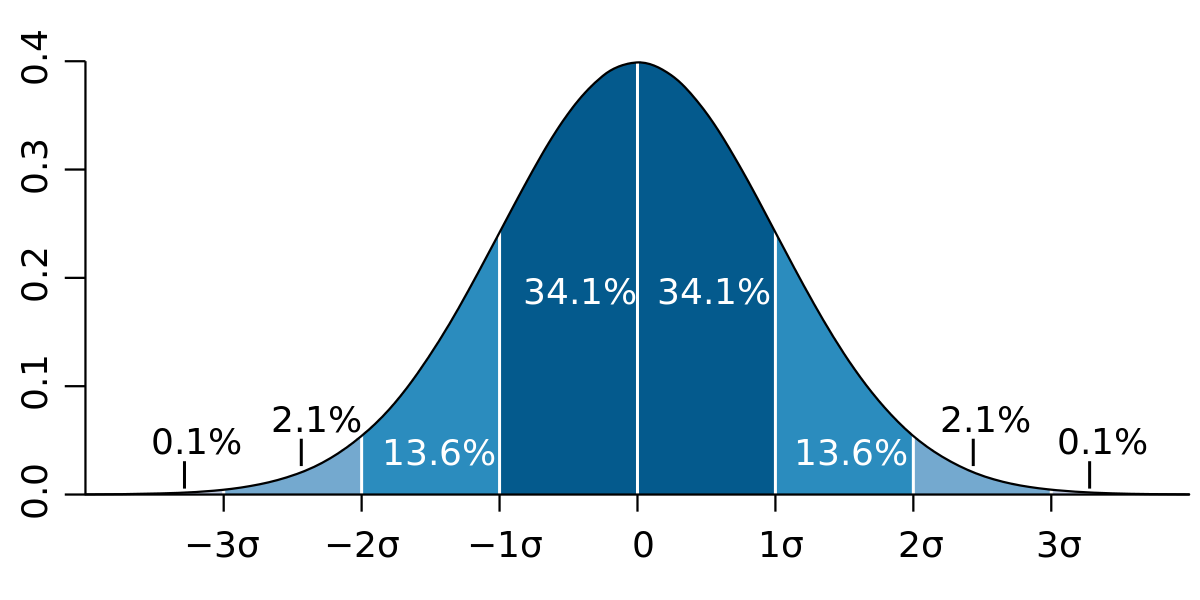
\includegraphics{Standard_deviation_diagram.svg.png}
\caption{Confidence interval graphical explanation}
\end{figure}

A Confidence Interval is a range of values we are fairly sure our true value lies in.

men running
Example: Average Height
We measure the heights of 40 randomly chosen men, and get a mean height of 175cm,

We also know the standard deviation of men's heights is 20cm.

The 95% Confidence Interval (we show how to calculate it later) is:

175cm � 6.2cm

confidence interval 175 plus minus 6.2

This says the true mean of ALL men (if we could measure all their heights) is likely to be between 168.8cm and 181.2cm.

But it might not be!

The "95%" says that 95% of experiments like we just did will include the true mean, but 5% won't.

So there is a 1-in-20 chance (5%) that our Confidence Interval does NOT include the true mean.





Step 1: start with

the number of observations n
the mean X
and the standard deviation s
Note: we should use the standard deviation of the entire population, but in many cases we won't know it.

We can use the standard deviation for the sample if we have enough observations (at least n=30, hopefully more).

Using our example:

number of observations n = 40
mean X = 175
standard deviation s = 20
Step 2: decide what Confidence Interval we want: 95% or 99% are common choices. Then find the "Z" value for that Confidence Interval here:

Confidence
Interval	Z
80%	1.282
85%	1.440
90%	1.645
95%	1.960
99%	2.576
99.5%	2.807
99.9%	3.291
For 95% the Z value is 1.960

Step 3: use that Z value in this formula for the Confidence Interval

X  �  Z s�n 

Where:

X is the mean
Z is the chosen Z-value from the table above
s is the standard deviation
n is the number of observations
And we have:

175 � 1.960 ?  20�40 

Which is:

175cm � 6.20cm

In other words: from 168.8cm to 181.2cm


Also from here is clear that increasing the number of experiments the confidence interval becomes narrower hence
how estimate is more precise.
 
\clearpage

%\chapter{Introduction to python}\label{introduction-to-python---lesson-1}

$\tt{Python}$ is one of the most widely used programming languages, and it has been around for more than 28 years now. 

First and foremost reason why $\tt{python}$ is much popular because it is highly productive as compared to other programming languages like $\tt{C++}$ and $\tt{java}$. It is a much more concise and expressive language and requires less time, effort, and lines of code to perform the same operations.

This makes $\tt{python}$ very easy-to-learn programming language even for beginners and newbies. It is also very famous for its simple programming syntax, code readability and English-like commands that make coding in Python lot easier and efficient.
With $\tt{python}$, the code looks very close to how humans think. For this purpose, it must abstract the details of the computer from you. Hence, it is slower than other “lower-level language” like $\tt{C}$.

There were times when computer run time was to be the main issue and the most expensive resource. But now, things have changed. Computer, servers and other hardware have become much much cheaper than ever and speed has become a less important factor. Today, development time matters more in most cases rather than execution speed. Reducing the time needed for each project saves companies tons of money.

As far as the execution speed or performance of the program is concerned, we can easily manage it by horizontal scaling, means getting more servers running to get that level of speed or performance.

In short, $\tt{python}$ is widely used even when it is somehow slower than other languages because:
\begin{itemize}
  \item is more productive;
  \item companies can optimize their most expensive resource: employees;
  \item rich set of libraries and frameworks;
  \item large community.
\end{itemize}

\section{What is $\tt{python}$ ?}\label{what-is-python}

$\tt{Python}$ is a so called \emph{interpreted language}: it takes some code (a sequence of instructions), reads and executes it. This is different from other programming languages like \texttt{C} or \texttt{C++} which \emph{compile} code into a language that the computer can understand directly (\emph{machine language}).

\begin{figure}[h]
\centering
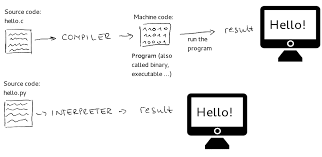
\includegraphics[width=0.7\linewidth]{index.png}
\caption{Interpreted vs compiled language}
\end{figure}

As a result, \(\tt{python}\) is essentially an \emph{interactive} programming language, you can program and see the results almost at the same time. This is very nice for a faster development since compilation time can be quite long (just to give an idea the compilation of our \texttt{C++} financial code takes more than one hour).
However there are drawbacks in terms of performance, the \emph{translation} to machine language has to be done in real-time resulting in slower execution times.

\begin{figure}[h]
\centering
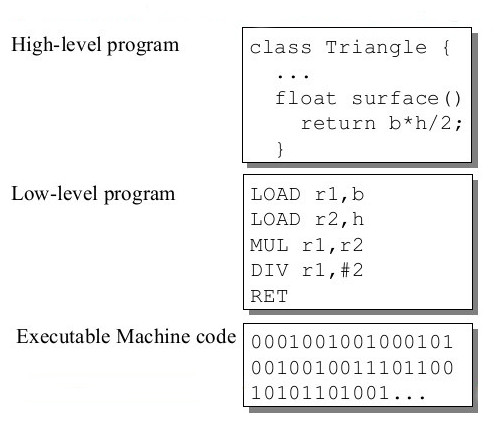
\includegraphics[width=0.5\linewidth]{machine_language.jpeg}
\caption{Human readable vs machine code}
\end{figure}

In the next chapters we'll take a quick tour of $\tt{python}$ and see the main features and characteristics of this programming language, later on we will see how it can be useful to solve real-world finance problems.

First of all since $\tt{python}$, as basically all programs, comes in different version and flavours we need to specify the particular one we are going to use.
The latest version (at the time I'm wrtiting this pages) is \(\tt{3.8.5}\), but it is continously evolving, however it is not difficult to see older versions floating around (e.g. \(\tt{2.7}\)).
This is because there are some big differences between \(\tt{python 2.X}\) and \(\tt{python 3.X}\) which prevent a sizeable portion of \(\tt{python 2}\) users to stick with it (consider that moving to \(\tt{python 3}\) would require a large amount of work to adapt big projects).
In conclusion we will concentrate on \textbf{\(\tt{python 3.7}\)}.

\section{$\tt{Python}$ basics}\label{python-basics}

Every language has \emph{keywords}, these are reserved words that have a special meaning and tell the computer what to do. The first one we encounter is \(\tt{print}\): it prints to screen whatever is specified between the parenthesis.

\begin{tcolorbox}[breakable, size=fbox, boxrule=1pt, pad at break*=1mm, colback=cellbackground, colframe=cellborder]
\begin{Verbatim}[commandchars=\\\{\}]
\PY{n+nb}{print} \PY{p}{(}\PY{l+s+s2}{\PYZdq{}}\PY{l+s+s2}{Hello world !}\PY{l+s+s2}{\PYZdq{}}\PY{p}{)} 

Hello world !
\end{Verbatim}
\end{tcolorbox}

\begin{tcolorbox}[breakable, size=fbox, boxrule=1pt, pad at break*=1mm, colback=cellbackground, colframe=cellborder]
\begin{Verbatim}[commandchars=\\\{\}]
\PY{n+nb}{print} \PY{p}{(}\PY{l+s+s2}{\PYZdq{}}\PY{l+s+s2}{Welcome}\PY{l+s+s2}{\PYZdq{}}\PY{p}{)}
\PY{n+nb}{print} \PY{p}{(}\PY{l+s+s2}{\PYZdq{}}\PY{l+s+s2}{to}\PY{l+s+s2}{\PYZdq{}}\PY{p}{)}
\PY{n+nb}{print} \PY{p}{(}\PY{l+s+s2}{\PYZdq{}}\PY{l+s+s2}{everybody}\PY{l+s+s2}{\PYZdq{}}\PY{p}{)}

Welcome
to
everybody
\end{Verbatim}
\end{tcolorbox}

Good programming practice recommends to document the code you write (you will soon see that it is surprisingly easy to forget what you wanted to do in your code). In \(\tt{python}\) you can add comments to code starting a line with a hash character (\#).

\begin{tcolorbox}[breakable, size=fbox, boxrule=1pt, pad at break*=1mm, colback=cellbackground, colframe=cellborder]
\begin{Verbatim}[commandchars=\\\{\}]
\PY{n+nb}{print} \PY{p}{(}\PY{l+s+s2}{\PYZdq{}}\PY{l+s+s2}{Ciao}\PY{l+s+s2}{\PYZdq{}}\PY{p}{)} \PY{c+c1}{\PYZsh{} this is a comment}

Ciao
\end{Verbatim}
\end{tcolorbox}

\subsection{Variables}\label{variables}

A variable is a computer memory location paired with an associated symbolic name, which contains some quantity of information referred to as a *value* (e.g.~a number, a string\ldots{}). Variables and hence data they contain, can be used, referenced and manipulated throughout a program.
A value is assigned to a variable with the equal operator (=). 

\begin{figure}[h]
\centering
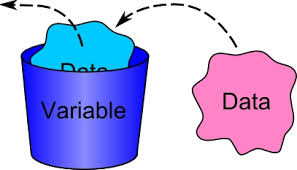
\includegraphics[width=0.5\linewidth]{var1.jpeg}
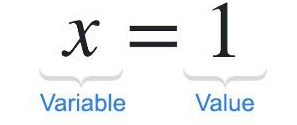
\includegraphics[width=0.5\linewidth]{var2.jpeg}
\caption{Graphical representation of a variable.}
\end{figure}

\begin{tcolorbox}[breakable, size=fbox, boxrule=1pt, pad at break*=1mm, colback=cellbackground, colframe=cellborder]
\begin{Verbatim}[commandchars=\\\{\}]
\PY{n}{x} \PY{o}{=} \PY{l+m+mi}{9}
\PY{n+nb}{print} \PY{p}{(}\PY{n}{x}\PY{p}{)}

9
\end{Verbatim}
\end{tcolorbox}

\begin{tcolorbox}[breakable, size=fbox, boxrule=1pt, pad at break*=1mm, colback=cellbackground, colframe=cellborder]
\begin{Verbatim}[commandchars=\\\{\}]
\PY{n}{myphone} \PY{o}{=} \PY{l+s+s2}{\PYZdq{}}\PY{l+s+s2}{Huawei P10Lite}\PY{l+s+s2}{\PYZdq{}}
\PY{n+nb}{print} \PY{p}{(}\PY{n}{myphone}\PY{p}{)}

Huawei P10Lite
\end{Verbatim}
\end{tcolorbox}

Another very useful keyword is \(\tt{type}\): it tells which kind of object is stored in a variable.

\begin{tcolorbox}[breakable, size=fbox, boxrule=1pt, pad at break*=1mm, colback=cellbackground, colframe=cellborder]
\begin{Verbatim}[commandchars=\\\{\}]
\PY{n+nb}{print} \PY{p}{(}\PY{n+nb}{type}\PY{p}{(}\PY{n}{x}\PY{p}{)}\PY{p}{)}
\PY{n+nb}{print} \PY{p}{(}\PY{n+nb}{type}\PY{p}{(}\PY{n}{myphone}\PY{p}{)}\PY{p}{)}

<class 'int'>
<class 'str'>
\end{Verbatim}
\end{tcolorbox}

After their definitions \(\tt{x}\) and \(\tt{myphone}\) can be used as aliases for a number and a string and their content manipulated, for example:

\begin{tcolorbox}[breakable, size=fbox, boxrule=1pt, pad at break*=1mm, colback=cellbackground, colframe=cellborder]
\begin{Verbatim}[commandchars=\\\{\}]
\PY{n+nb}{print} \PY{p}{(}\PY{n}{x}\PY{o}{+}\PY{l+m+mi}{5}\PY{p}{)}

14
\end{Verbatim}
\end{tcolorbox}

There are rules that limit the variable naming possibilities, in particular they must:
\begin{itemize}
\item begin with a letter (\tt{myphone}) or underscore (\tt{\_myphone});
\item other characters can be letters, numbers or more \_;
\item variable names are case-sensitive so \tt{myphone} and \tt{myPhone} are two distinct variables;
\end{itemize}

\textbf{Keywords, as said, are reserved words and as such cannot be used as variable names (e.g.~\(\tt{print, type, for...}\))}.

To use \textbf{good} variable names (and make you programs clearer and easier to read) always choose meaningful names instead of short names (i.e. \(\tt{numberOfCakes}\) is much better than simply \(\tt{n}\)), try to be consistent with your conventions (e.g.~choose once and for all between \(\tt{number\_of\_cakes}\) or
\(\tt{numberofcakes}\) or \(\tt{numberOfCakes}\)), usually begin a variable name with underscore (\_) only for a special case (will see later when this is usually done).

\subsection{Boolean expressions}\label{boolean-expressions}

Boolean expressions evaluate to \(\tt{true}\) or \(\tt{false}\) only. This type
of expressions usually involve logical or comparison operators like \(\tt{or}\), \(\tt{and}\), \textgreater{} (greater than), \textless{} (less than)\ldots{}
The equal boolean operator symbol is a double = (==), to not be confused with the assignement operator single = (=), with the first we compare two variables, with the second we associate a value to a variable.

Let's see some example. The following expression answer the question is 1 equal to 2:

\begin{tcolorbox}[breakable, size=fbox, boxrule=1pt, pad at break*=1mm, colback=cellbackground, colframe=cellborder]
\begin{Verbatim}[commandchars=\\\{\}]
\PY{l+m+mi}{1} \PY{o}{==} \PY{l+m+mi}{2} 

False
\end{Verbatim}
\end{tcolorbox}

Here another example using the not equal operator (!=):

\begin{tcolorbox}[breakable, size=fbox, boxrule=1pt, pad at break*=1mm, colback=cellbackground, colframe=cellborder]
\begin{Verbatim}[commandchars=\\\{\}]

True
\end{Verbatim}
\end{tcolorbox}

\begin{tcolorbox}[breakable, size=fbox, boxrule=1pt, pad at break*=1mm, colback=cellbackground, colframe=cellborder]
\begin{Verbatim}[commandchars=\\\{\}]
\PY{l+m+mi}{2} \PY{o}{\PYZlt{}} \PY{l+m+mi}{2}

False
\end{Verbatim}
\end{tcolorbox}

\begin{tcolorbox}[breakable, size=fbox, boxrule=1pt, pad at break*=1mm, colback=cellbackground, colframe=cellborder]
\begin{Verbatim}[commandchars=\\\{\}]
\PY{l+m+mi}{2} \PY{o}{\PYZlt{}}\PY{o}{=} \PY{l+m+mi}{2}  \PY{c+c1}{\PYZsh{} in this case we allow the numbers to be equal too}

True
\end{Verbatim}
\end{tcolorbox}

\begin{tcolorbox}[breakable, size=fbox, boxrule=1pt, pad at break*=1mm, colback=cellbackground, colframe=cellborder]
\begin{Verbatim}[commandchars=\\\{\}]
\PY{n+nb}{print} \PY{p}{(}\PY{n}{x}\PY{p}{)}
\PY{l+m+mi}{15} \PY{o}{\PYZlt{}}\PY{o}{=} \PY{n}{x} \PY{o+ow}{and} \PY{n}{x} \PY{o}{\PYZlt{}}\PY{o}{=} \PY{l+m+mi}{20} \PY{c+c1}{\PYZsh{} this expression could also be written as 15 \PYZlt{}= x \PYZlt{}= 20}

11
False
\end{Verbatim}
\end{tcolorbox}

\begin{tcolorbox}[breakable, size=fbox, boxrule=1pt, pad at break*=1mm, colback=cellbackground, colframe=cellborder]            
\begin{Verbatim}[commandchars=\\\{\}]
\PY{l+m+mi}{15} \PY{o}{\PYZlt{}}\PY{o}{=} \PY{n}{x} \PY{o+ow}{or} \PY{n}{x} \PY{o}{\PYZlt{}}\PY{o}{=} \PY{l+m+mi}{20}

True
\end{Verbatim}
\end{tcolorbox}

\begin{tcolorbox}[breakable, size=fbox, boxrule=1pt, pad at break*=1mm, colback=cellbackground, colframe=cellborder]            
\begin{Verbatim}[commandchars=\\\{\}]
\PY{o+ow}{not} \PY{p}{(}\PY{n}{x} \PY{o}{\PYZgt{}} \PY{l+m+mi}{20}\PY{p}{)} \PY{c+c1}{\PYZsh{} the not keyword negates the following expression}

True
\end{Verbatim}
\end{tcolorbox}

\subsection{String expressions}\label{string-expressions}

A ``string'' is a sequence of characters (letters, digits, spaces, punctuation\ldots{}). There are many operations that can be performed on strings, like for example concatenate (with + operator), truncate, replace characters\ldots{}

\begin{tcolorbox}[breakable, size=fbox, boxrule=1pt, pad at break*=1mm, colback=cellbackground, colframe=cellborder]            
\begin{Verbatim}[commandchars=\\\{\}]
\PY{n}{mystring} \PY{o}{=} \PY{l+s+s2}{\PYZdq{}}\PY{l+s+s2}{some text with punctuation, spaces and digits 10}\PY{l+s+s2}{\PYZdq{}}
\PY{n}{mystring}\PY{o}{.}\PY{n}{replace}\PY{p}{(}\PY{l+s+s2}{\PYZdq{}}\PY{l+s+s2}{s}\PY{l+s+s2}{\PYZdq{}}\PY{p}{,} \PY{l+s+s2}{\PYZdq{}}\PY{l+s+s2}{z}\PY{l+s+s2}{\PYZdq{}}\PY{p}{)}

'zome text with punctuation, zpacez and digitz 10'
\end{Verbatim}
\end{tcolorbox}

\begin{tcolorbox}[breakable, size=fbox, boxrule=1pt, pad at break*=1mm, colback=cellbackground, colframe=cellborder]            
\begin{Verbatim}[commandchars=\\\{\}]
\PY{l+s+s2}{\PYZdq{}}\PY{l+s+s2}{abc}\PY{l+s+s2}{\PYZdq{}} \PY{o}{+} \PY{l+s+s2}{\PYZdq{}}\PY{l+s+s2}{def}\PY{l+s+s2}{\PYZdq{}} \PY{c+c1}{\PYZsh{} it is possible to concatenate strings with + }

'abcdef'
\end{Verbatim}
\end{tcolorbox}

\begin{tcolorbox}[breakable, size=fbox, boxrule=1pt, pad at break*=1mm, colback=cellbackground, colframe=cellborder]            
\begin{Verbatim}[commandchars=\\\{\}]
\PY{l+s+s2}{\PYZdq{}}\PY{l+s+s2}{The number }\PY{l+s+s2}{\PYZdq{}} \PY{o}{+} \PY{l+m+mi}{4} \PY{o}{+} \PY{l+s+s2}{\PYZdq{}}\PY{l+s+s2}{ is my favourite number}\PY{l+s+s2}{\PYZdq{}}
\PY{c+c1}{\PYZsh{} this causes an error since we are trying to concatenate a string }
\PY{c+c1}{\PYZsh{} with a number so two different kind of objects}

---------------------------------------------------------------------------

TypeError                                 Traceback (most recent call last)

<ipython-input-33-b9f65c5a45f7> in <module>()
----> 1 "The number " + 4 + " is my favourite number"
      2 \# this causes an error since we are trying to concatenate a string
      3 \# with a number so two different kind of objects

TypeError: can only concatenate str (not "int") to str
\end{Verbatim}
\end{tcolorbox}

To avoid this error is possible to \textbf{cast} an object to a different type which means to convert an object to a different type. In this case we can \emph{force} the number four to be represented as a string with the \(\tt{str()}\) function:

\begin{tcolorbox}[breakable, size=fbox, boxrule=1pt, pad at break*=1mm, colback=cellbackground, colframe=cellborder]            
\begin{Verbatim}[commandchars=\\\{\}]
\PY{l+s+s2}{\PYZdq{}}\PY{l+s+s2}{The number }\PY{l+s+s2}{\PYZdq{}} \PY{o}{+} \PY{n+nb}{str}\PY{p}{(}\PY{l+m+mi}{4}\PY{p}{)} \PY{o}{+} \PY{l+s+s2}{\PYZdq{}}\PY{l+s+s2}{ is my favourite number}\PY{l+s+s2}{\PYZdq{}}

'The number 4 is my favourite number'
\end{Verbatim}
\end{tcolorbox}

\begin{tcolorbox}[breakable, size=fbox, boxrule=1pt, pad at break*=1mm, colback=cellbackground, colframe=cellborder]            
\begin{Verbatim}[commandchars=\\\{\}]
\PY{n+nb}{print} \PY{p}{(}\PY{n+nb}{type}\PY{p}{(}\PY{l+m+mf}{3.4}\PY{p}{)}\PY{p}{)}
\PY{n+nb}{print} \PY{p}{(}\PY{n+nb}{type}\PY{p}{(}\PY{n+nb}{str}\PY{p}{(}\PY{l+m+mf}{3.4}\PY{p}{)}\PY{p}{)}\PY{p}{)}

<class 'float'>
<class 'str'>
\end{Verbatim}
\end{tcolorbox}

In this simple case everything worked fine but type casting is not always possible: for example a number can be converted to a string (e.g.~from the integer 4 to the actual symbol ``4'') but the opposite is not possible (e.g.~cannot convert the string ``matteo'' to a meaningful number). In this second case we can try to use the function \(\tt{int()}\) to convert a string to an integer.

\begin{tcolorbox}[breakable, size=fbox, boxrule=1pt, pad at break*=1mm, colback=cellbackground, colframe=cellborder]            
\begin{Verbatim}[commandchars=\\\{\}]
\PY{n+nb}{int}\PY{p}{(}\PY{l+s+s2}{\PYZdq{}}\PY{l+s+s2}{matteo}\PY{l+s+s2}{\PYZdq{}}\PY{p}{)}

---------------------------------------------------------------------------

ValueError                                Traceback (most recent call last)

<ipython-input-17-979283bb65e4> in <module>
----> 1 int("matteo")  

ValueError: invalid literal for int() with base 10: 'matteo'
\end{Verbatim}
\end{tcolorbox}

\begin{tcolorbox}[breakable, size=fbox, boxrule=1pt, pad at break*=1mm, colback=cellbackground, colframe=cellborder]            
\begin{Verbatim}[commandchars=\\\{\}]
\PY{n+nb}{int}\PY{p}{(}\PY{l+s+s2}{\PYZdq{}}\PY{l+s+s2}{4}\PY{l+s+s2}{\PYZdq{}}\PY{p}{)}

4
\end{Verbatim}
\end{tcolorbox}

\paragraph{Pretty string formatting: } in order to get prettier strings than those obtained just concatenating with the + operator, \(\tt{python}\) allows to format text using the following syntax ``text {} other text''.format(variable).
With this notation, each {} is mapped to the variables listed in the $\tt{format}$ statement, the optional characters inside the curly brackets can determine the resulting format, for example in the following code $\tt{:.1f}$ means that this variable is float number and that has to be printed with 1 digit only after the decimal separator. 

\begin{tcolorbox}[breakable, size=fbox, boxrule=1pt, pad at break*=1mm, colback=cellbackground, colframe=cellborder]            
\begin{Verbatim}[commandchars=\\\{\}]
\PY{l+s+s2}{\PYZdq{}}\PY{l+s+s2}{The speed of light is about }\PY{l+s+si}{\PYZob{}:.1f\PYZcb{}}\PY{l+s+s2}{ }\PY{l+s+si}{\PYZob{}\PYZcb{}}\PY{l+s+s2}{\PYZdq{}}\PY{o}{.}\PY{n}{format}\PY{p}{(}\PY{l+m+mf}{299792.458}\PY{p}{,} \PY{l+s+s2}{\PYZdq{}}\PY{l+s+s2}{km/s}\PY{l+s+s2}{\PYZdq{}}\PY{p}{)}

'The speed of light is about 299792.5 km/s'
\end{Verbatim}
\end{tcolorbox}

In addition $\tt{format}$ allows for 0-padding of numbers, left or right alignement of text columns and so on.

\subsection{Mathematical expressions}\label{mathematical-expressions}

Below few examples of the basic mathematical expressions available in $\tt{python}$.

\begin{tcolorbox}[breakable, size=fbox, boxrule=1pt, pad at break*=1mm, colback=cellbackground, colframe=cellborder]            
\begin{Verbatim}[commandchars=\\\{\}]
\PY{l+m+mi}{1} \PY{o}{+} \PY{l+m+mi}{2}

3
\end{Verbatim}
\end{tcolorbox}

\begin{tcolorbox}[breakable, size=fbox, boxrule=1pt, pad at break*=1mm, colback=cellbackground, colframe=cellborder]            
\begin{Verbatim}[commandchars=\\\{\}]
\PY{l+m+mi}{40} \PY{o}{\PYZhy{}} \PY{l+m+mi}{5}

35
\end{Verbatim}
\end{tcolorbox}

\begin{tcolorbox}[breakable, size=fbox, boxrule=1pt, pad at break*=1mm, colback=cellbackground, colframe=cellborder]            
\begin{Verbatim}[commandchars=\\\{\}]
\PY{n}{x} \PY{o}{*} \PY{l+m+mi}{20} \PY{c+c1}{\PYZsh{} remember that we set x equal to 9}

180
\end{Verbatim}
\end{tcolorbox}

\begin{tcolorbox}[breakable, size=fbox, boxrule=1pt, pad at break*=1mm, colback=cellbackground, colframe=cellborder]            
\begin{Verbatim}[commandchars=\\\{\}]
\PY{n}{x} \PY{o}{/} \PY{l+m+mi}{4}

2.25
\end{Verbatim}
\end{tcolorbox}

\begin{tcolorbox}[breakable, size=fbox, boxrule=1pt, pad at break*=1mm, colback=cellbackground, colframe=cellborder]            
\begin{Verbatim}[commandchars=\\\{\}]
\PY{n+nb}{print} \PY{p}{(}\PY{n+nb}{type}\PY{p}{(}\PY{l+m+mf}{2.25}\PY{p}{)}\PY{p}{)}

<class 'float'>
\end{Verbatim}
\end{tcolorbox}

\begin{tcolorbox}[breakable, size=fbox, boxrule=1pt, pad at break*=1mm, colback=cellbackground, colframe=cellborder]            
\begin{Verbatim}[commandchars=\\\{\}]
\PY{n}{x} \PY{o}{/}\PY{o}{/} \PY{l+m+mi}{4} \PY{c+c1}{\PYZsh{} interger division \PYZhy{} result will be truncated to the }
       \PY{c+c1}{\PYZsh{} corresponding integer (no rounding)}
       \PY{c+c1}{\PYZsh{} 11 / 3 = 3.666666 \PYZhy{}\PYZgt{} 11 // 3 = 3}

2
\end{Verbatim}
\end{tcolorbox}

\begin{tcolorbox}[breakable, size=fbox, boxrule=1pt, pad at break*=1mm, colback=cellbackground, colframe=cellborder]            
\begin{Verbatim}[commandchars=\\\{\}]
\PY{n}{y} \PY{o}{=} \PY{l+m+mi}{3}
\PY{n}{x} \PY{o}{*}\PY{o}{*} \PY{n}{y} \PY{c+c1}{\PYZsh{} x to the power of y}

729
\end{Verbatim}
\end{tcolorbox}

\begin{tcolorbox}[breakable, size=fbox, boxrule=1pt, pad at break*=1mm, colback=cellbackground, colframe=cellborder]            
\begin{Verbatim}[commandchars=\\\{\}]
\PY{l+m+mi}{3} \PY{o}{*} \PY{p}{(}\PY{n}{x} \PY{o}{+} \PY{n}{y}\PY{p}{)}

36
\end{Verbatim}
\end{tcolorbox}

As an example of variable manipulation let's try to increment \(\tt{x}\) by 1 and save the result again in \(\tt{x}\).

\begin{tcolorbox}[breakable, size=fbox, boxrule=1pt, pad at break*=1mm, colback=cellbackground, colframe=cellborder]            
\begin{Verbatim}[commandchars=\\\{\}]
\PY{n+nb}{print} \PY{p}{(}\PY{n}{x}\PY{p}{)}
\PY{n}{x} \PY{o}{=} \PY{n}{x} \PY{o}{+} \PY{l+m+mi}{1}
\PY{n+nb}{print} \PY{p}{(}\PY{n}{x}\PY{p}{)}

15
16
\end{Verbatim}
\end{tcolorbox}

Sometimes the increment of a variable plus the assignment to the same variable is written with a more compact syntax \texttt{x += 1} (this is also true for other operators e.g. \texttt{x *= 2}).

More complex mathematical functions are not directly available, let's see for example the logarithm:

\begin{tcolorbox}[breakable, size=fbox, boxrule=1pt, pad at break*=1mm, colback=cellbackground, colframe=cellborder]            
\begin{Verbatim}[commandchars=\\\{\}]
\PY{n}{log}\PY{p}{(}\PY{l+m+mi}{3}\PY{p}{)}

---------------------------------------------------------------------------

NameError                                 Traceback (most recent call last)

<ipython-input-17-ffde4d60496a> in <module>()
    ----> 1 log(3) \# causes an error because the logarithm function
          2        \# is not available by default


NameError: name 'log' is not defined
\end{Verbatim}
\end{tcolorbox}

\section{Modules}\label{modules}

One very important feature of each language is the ability to reuse code among different programs, e.g.~imagine how awful would be if you had to reimplement every time you need it a function to compute the logarithm.
Usually there are mechanisms that allow to collect useful routines in \emph{packages} (or \emph{libraries}, or \emph{modules}) so that later they can be called and used by any program may need them.

These collections of utilities in \(\tt{python}\) are called \emph{modules} and each installation of this language brings with it a standard set of them. If you need more functionality, you can download more modules from the web (there are zillions out there) or if you are not satisfied with what you found you can write your own (which is one the goal of this course in the end).

Some examples of useful modules we will use are:

\begin{itemize}
\tightlist
\item
  Numpy - which provides matrix algebra functionality and much more;
\item
  Scipy - which provides a whole series of scientific computing
  functions;
\item
  Pandas - which provides tools for manipulating time series or dataset
  in general;
\item
  Matplotlib - for plotting graphs;
\item
  Jupyter - for notebooks like this one.
\end{itemize}

\begin{figure}
\centering
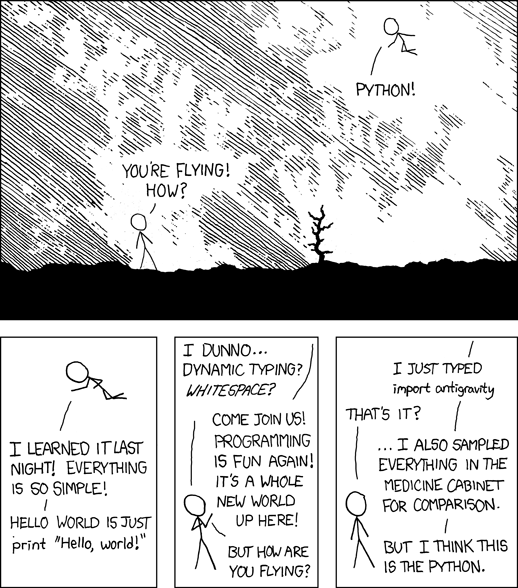
\includegraphics[width=0.75\linewidth]{python.png}
\caption{$\tt{Python}$ has many modules for download on the web\ldots{}}
\end{figure}

Later we will take a closer look at three modules which are quite useful in financial analysis.

In order to load a module in a \(\tt{python}\) program you can use the \(\tt{import}\) keyword. To inspect a module (to understand which are its functionalities) it can be used the \(\tt{help}\) and \(\tt{dir}\) keywords: the first write a help message which usually describes the functionalities of a module, the latter list all the available functions of a module.
\textbf{In order to access a function of a module you have to use the . (dot) operator: module-name.function-name.}

Let's see an example dealing with the\(\tt{math}\) module which implements the most common mathematical functions.

\begin{tcolorbox}[breakable, size=fbox, boxrule=1pt, pad at break*=1mm, colback=cellbackground, colframe=cellborder]            
\begin{Verbatim}[commandchars=\\\{\}]
\PY{k+kn}{import} \PY{n+nn}{math}
\PY{n+nb}{dir}\PY{p}{(}\PY{n}{math}\PY{p}{)}

{\color{outcolor}Out[{\color{outcolor}18}]:} ['\_\_doc\_\_',
          '\_\_loader\_\_',
          '\_\_name\_\_',
          '\_\_package\_\_',
          '\_\_spec\_\_',
          'acos',
          'acosh',
          'asin',
          'asinh',
          'atan',
          'atan2',
          'atanh',
          'ceil',
          'copysign',
          'cos',
          'cosh',
...
\end{Verbatim}
\end{tcolorbox}

\begin{tcolorbox}[breakable, size=fbox, boxrule=1pt, pad at break*=1mm, colback=cellbackground, colframe=cellborder]            
\begin{Verbatim}[commandchars=\\\{\}]
\PY{n+nb}{help}\PY{p}{(}\PY{n}{math}\PY{p}{)}

Help on module math:

NAME
    math

MODULE REFERENCE
    https://docs.python.org/3.6/library/math

    The following documentation is automatically generated from the Python
    source files.  It may be incomplete, incorrect or include features that
    are considered implementation detail and may vary between Python
    implementations.  When in doubt, consult the module reference at the
    location listed above.

DESCRIPTION
    This module is always available.  It provides access to the
    mathematical functions defined by the C standard.

FUNCTIONS
    acos({\ldots})
        acos(x)

        Return the arc cosine (measured in radians) of x.
...
\end{Verbatim}
\end{tcolorbox}

\begin{tcolorbox}[breakable, size=fbox, boxrule=1pt, pad at break*=1mm, colback=cellbackground, colframe=cellborder]            
\begin{Verbatim}[commandchars=\\\{\}]
\PY{n}{math}\PY{o}{.}\PY{n}{log}\PY{p}{(}\PY{l+m+mi}{3}\PY{p}{)}

1.0986122886681098
\end{Verbatim}
\end{tcolorbox}

\begin{tcolorbox}[breakable, size=fbox, boxrule=1pt, pad at break*=1mm, colback=cellbackground, colframe=cellborder]            
\begin{Verbatim}[commandchars=\\\{\}]
\PY{n}{math}\PY{o}{.}\PY{n}{exp}\PY{p}{(}\PY{l+m+mi}{3}\PY{p}{)}

20.085536923187668
\end{Verbatim}
\end{tcolorbox}

\begin{tcolorbox}[breakable, size=fbox, boxrule=1pt, pad at break*=1mm, colback=cellbackground, colframe=cellborder]            
\begin{Verbatim}[commandchars=\\\{\}]
\PY{n+nb}{print} \PY{p}{(}\PY{n+nb}{type}\PY{p}{(}\PY{n}{math}\PY{o}{.}\PY{n}{log}\PY{p}{)}\PY{p}{)} \PY{c+c1}{\PYZsh{} yet another type: builtin function}
\PY{n+nb}{print} \PY{p}{(}\PY{n+nb}{type}\PY{p}{(}\PY{n}{math}\PY{o}{.}\PY{n}{log}\PY{p}{(}\PY{l+m+mi}{3}\PY{p}{)}\PY{p}{)}\PY{p}{)}

<class 'builtin\_function\_or\_method'>
<class 'float'>
\end{Verbatim}
\end{tcolorbox}

If we want to avoid to type ``math.'' every time we compute a logarithm or an exponential, we can just import the needed functions from a module using the following syntax:

\begin{tcolorbox}[breakable, size=fbox, boxrule=1pt, pad at break*=1mm, colback=cellbackground, colframe=cellborder]            
\begin{Verbatim}[commandchars=\\\{\}]
\PY{k+kn}{from} \PY{n+nn}{math} \PY{k}{import} \PY{n}{log}\PY{p}{,} \PY{n}{exp}
\PY{n+nb}{print} \PY{p}{(}\PY{n}{log}\PY{p}{(}\PY{l+m+mi}{3}\PY{p}{)}\PY{p}{)}
\PY{n+nb}{print} \PY{p}{(}\PY{n}{exp}\PY{p}{(}\PY{l+m+mi}{3}\PY{p}{)}\PY{p}{)}

1.0986122886681098
20.085536923187668
\end{Verbatim}
\end{tcolorbox}

As an example let's compute the interest rate \(r\) that produces a return \(R\) of 11000 Euro when investing 10000 Euro for 2 years:

\(R = N\mathrm{e}^{r\tau} \rightarrow r = \frac{1}{\tau} \mathrm{log}(\frac{R}{N})\)

\begin{tcolorbox}[breakable, size=fbox, boxrule=1pt, pad at break*=1mm, colback=cellbackground, colframe=cellborder]            
\begin{Verbatim}[commandchars=\\\{\}]
\PY{n}{rate} \PY{o}{=} \PY{p}{(}\PY{l+m+mi}{1}\PY{o}{/}\PY{l+m+mi}{2}\PY{p}{)}\PY{o}{*}\PY{n}{log}\PY{p}{(}\PY{l+m+mf}{11000}\PY{o}{/}\PY{l+m+mi}{10000}\PY{p}{)}
\PY{n+nb}{print} \PY{p}{(}\PY{n}{rate}\PY{p}{)}

0.04765508990216247
\end{Verbatim}
\end{tcolorbox}

\section{Indented blocks and the $\tt{if/else}$ statement}\label{indented-blocks-and-the-ttifelse-statement}

Unlike other languages which uses parenthesis to isolate blocks of code $\tt{python}$ uses indentation. A first example of this is given by $\tt{if/then}$ statements. Such commands allow to dynamically run different blocks of code based on certain conditions. For example in the following we print different statements according to the value of $\tt{x}$, note the that the block of code to be run according each condition is shifted (i.e.~indented) with respect to the rest of the
code:

\begin{tcolorbox}[breakable, size=fbox, boxrule=1pt, pad at break*=1mm, colback=cellbackground, colframe=cellborder]            
\begin{Verbatim}[commandchars=\\\{\}]
\PY{n+nb}{print} \PY{p}{(}\PY{n}{x}\PY{p}{)}
\PY{k}{if} \PY{n}{x} \PY{o}{==} \PY{l+m+mi}{1}\PY{p}{:} 
    \PY{n+nb}{print} \PY{p}{(}\PY{l+s+s2}{\PYZdq{}}\PY{l+s+s2}{This will not be printed}\PY{l+s+s2}{\PYZdq{}}\PY{p}{)} 
    \PY{c+c1}{\PYZsh{} the block of code that is run if the first condition is met is indented}
\PY{k}{elif} \PY{n}{x} \PY{o}{==} \PY{l+m+mi}{15}\PY{p}{:}
    \PY{n+nb}{print} \PY{p}{(}\PY{l+s+s2}{\PYZdq{}}\PY{l+s+s2}{This will not be printed either}\PY{l+s+s2}{\PYZdq{}}\PY{p}{)}
    \PY{c+c1}{\PYZsh{} again the block of code that is run here is indented}
    \PY{c+c1}{\PYZsh{} to be \PYZdq{}isolated\PYZdq{} by the rest }
\PY{k}{else}\PY{p}{:}
    \PY{n+nb}{print} \PY{p}{(}\PY{l+s+s2}{\PYZdq{}}\PY{l+s+s2}{This *will* be printed}\PY{l+s+s2}{\PYZdq{}}\PY{p}{)}

16
This *will* be printed
\end{Verbatim}
\end{tcolorbox}

If by mistake the indentation of a block is missing an error is raised:
\begin{tcolorbox}[breakable, size=fbox, boxrule=1pt, pad at break*=1mm, colback=cellbackground, colframe=cellborder]            
\begin{Verbatim}[commandchars=\\\{\}]
\PY{k}{if} \PY{n}{x} \PY{o}{==} \PY{l+m+mi}{1}\PY{p}{:} 
\PY{n+nb}{print} \PY{p}{(}\PY{l+s+s2}{\PYZdq{}}\PY{l+s+s2}{This will not be printed}\PY{l+s+s2}{\PYZdq{}}\PY{p}{)}
\PY{k}{elif} \PY{n}{x} \PY{o}{==} \PY{l+m+mi}{15}\PY{p}{:}
    \PY{n+nb}{print} \PY{p}{(}\PY{l+s+s2}{\PYZdq{}}\PY{l+s+s2}{This will not be printed either}\PY{l+s+s2}{\PYZdq{}}\PY{p}{)}
\PY{k}{else}\PY{p}{:}
    \PY{n+nb}{print} \PY{p}{(}\PY{l+s+s2}{\PYZdq{}}\PY{l+s+s2}{This *will* be printed}\PY{l+s+s2}{\PYZdq{}}\PY{p}{)}

File "<ipython-input-38-4535a45a6419>", line 3
  print ("This will not be printed")
    \^{}
IndentationError: expected an indented block
\end{Verbatim}
\end{tcolorbox}

Below another example:
\begin{tcolorbox}[breakable, size=fbox, boxrule=1pt, pad at break*=1mm, colback=cellbackground, colframe=cellborder]            
\begin{Verbatim}[commandchars=\\\{\}]
\PY{k}{if} \PY{n}{x} \PY{o}{!=} \PY{l+m+mi}{1}\PY{p}{:}
   \PY{n+nb}{print} \PY{p}{(}\PY{l+s+s2}{\PYZdq{}}\PY{l+s+s2}{x does not equal to 1}\PY{l+s+s2}{\PYZdq{}}\PY{p}{)}

x does not equal to 1
\end{Verbatim}
\end{tcolorbox}

Just for comparison this is the same code written in $\tt{C++}$:

\begin{Shaded}
\begin{Highlighting}[]
\ControlFlowTok{if}\NormalTok{ (x == }\DecValTok{1}\NormalTok{) \{}
\NormalTok{ print (}\StringTok{"This will not be printed"}\NormalTok{);}
\NormalTok{\}}
\ControlFlowTok{else} \ControlFlowTok{if}\NormalTok{ (x == }\DecValTok{15}\NormalTok{) \{}
\NormalTok{  print (}\StringTok{"This will not be printed either"}\NormalTok{);}
\NormalTok{\}}
\ControlFlowTok{else}\NormalTok{ \{}
\NormalTok{print (}\StringTok{"This *will* be printed"}\NormalTok{);}
\NormalTok{\}}
\end{Highlighting}
\end{Shaded}

N.B. Notice how indentation doesn't matter at all here since the blocks are enclosed and defined by the brackets.

\section{Loops}\label{loops}

Another very important feature of a language is the ability to repeatedly run the same block of code many times. These is called looping and in \(\tt{python}\) can be done with $\tt{for}$ or $\tt{while}$ keywords.

\subsection{for}\label{for}

In a $\tt{for}$ loop we specifiy the set (or interval) over which we want to loop and a variable will assume all the values in that set (or interval). For example let's assume we want to print all the numbers between 25 and 30 excluded (here the keyword $\tt{range}$ returns the list of integers between the specified limits, if the first limit is not specified 0 is assumed):

\begin{tcolorbox}[breakable, size=fbox, boxrule=1pt, pad at break*=1mm, colback=cellbackground, colframe=cellborder]            
\begin{Verbatim}[commandchars=\\\{\}]
\PY{k}{for} \PY{n}{i} \PY{o+ow}{in} \PY{n+nb}{range}\PY{p}{(}\PY{l+m+mi}{25}\PY{p}{,} \PY{l+m+mi}{30}\PY{p}{)}\PY{p}{:}
     \PY{n+nb}{print} \PY{p}{(}\PY{n}{i}\PY{p}{)}

25
26
27
28
29
\end{Verbatim}
\end{tcolorbox}

At each cycle of the loop the variable $\tt{i}$ takes one of the values between
25 and 31. With $\tt{range}$ it is also possible to specify the step, so that the loop can jump every 2 units or to go in descending order:

\begin{tcolorbox}[breakable, size=fbox, boxrule=1pt, pad at break*=1mm, colback=cellbackground, colframe=cellborder]            
\begin{Verbatim}[commandchars=\\\{\}]
\PY{k}{for} \PY{n}{i} \PY{o+ow}{in} \PY{n+nb}{range} \PY{p}{(}\PY{l+m+mi}{30}\PY{p}{,} \PY{l+m+mi}{25}\PY{p}{,} \PY{o}{\PYZhy{}}\PY{l+m+mi}{1}\PY{p}{)}\PY{p}{:}
    \PY{n+nb}{print} \PY{p}{(}\PY{n}{i}\PY{p}{)}

30
29
28
27
26
\end{Verbatim}
\end{tcolorbox}

If it is needed to skip values in the loop the $\tt{continue}$ keyword can be used; in the code below 5 is actually missing from the list in the printout since it has been skipped by the $\tt{continue}$:

\begin{tcolorbox}[breakable, size=fbox, boxrule=1pt, pad at break*=1mm, colback=cellbackground, colframe=cellborder]            
\begin{Verbatim}[commandchars=\\\{\}]
\PY{k}{for} \PY{n}{i} \PY{o+ow}{in} \PY{n+nb}{range}\PY{p}{(}\PY{l+m+mi}{10}\PY{p}{)}\PY{p}{:}
    \PY{k}{if} \PY{n}{i} \PY{o}{==} \PY{l+m+mi}{5}\PY{p}{:}
        \PY{k}{continue} 
    \PY{n+nb}{print} \PY{p}{(}\PY{n}{i}\PY{p}{)}

0
1
2
3
4
6
7
8
9
\end{Verbatim}
\end{tcolorbox}

Instead of using $\tt{range}$ it is possbile to specify directly the set of looping values:

\begin{tcolorbox}[breakable, size=fbox, boxrule=1pt, pad at break*=1mm, colback=cellbackground, colframe=cellborder]            

\begin{Verbatim}[commandchars=\\\{\}]
\PY{k}{for} \PY{n}{i} \PY{o+ow}{in} \PY{p}{(}\PY{l+m+mi}{4}\PY{p}{,} \PY{l+m+mi}{6}\PY{p}{,} \PY{l+m+mi}{10}\PY{p}{,} \PY{l+m+mi}{20}\PY{p}{)}\PY{p}{:} \PY{c+c1}{\PYZsh{} here we loop directly on a list of numbers}
   \PY{n+nb}{print} \PY{p}{(}\PY{n}{i}\PY{p}{)}

4
6
10
20
\end{Verbatim}
\end{tcolorbox}

Finally looping on a string actually means to loop on each single character:
 
\begin{tcolorbox}[breakable, size=fbox, boxrule=1pt, pad at break*=1mm, colback=cellbackground, colframe=cellborder]            
\begin{Verbatim}[commandchars=\\\{\}]
\PY{n}{phrase} \PY{o}{=} \PY{l+s+s1}{\PYZsq{}}\PY{l+s+s1}{how to loop over a string}\PY{l+s+s1}{\PYZsq{}}
\PY{k}{for} \PY{n}{c} \PY{o+ow}{in} \PY{n}{phrase}\PY{p}{:}
   \PY{n+nb}{print} \PY{p}{(}\PY{n}{c}\PY{p}{)}

h
o
w
 
t
o
 
l
o
o
p
 
o
v
e
r
 
a
 
s
t
r
i
n
g
\end{Verbatim}
\end{tcolorbox}

\subsection{while}\label{while}

In a $\tt{for}$ loop we go through all the elements of a list of objects, the \texttt{while} statement instead repeats the same block of code untill a condition is met.
The following block of code is run if \texttt{x} squared is less than 50, so we first set \texttt{x=1} and at each iteration we increment it by 1 untill the condition is \texttt{True} (8 squared is 64 which is greater than 50):

\begin{tcolorbox}[breakable, size=fbox, boxrule=1pt, pad at break*=1mm, colback=cellbackground, colframe=cellborder]            
\begin{Verbatim}[commandchars=\\\{\}]
\PY{n}{x} \PY{o}{=} \PY{l+m+mi}{1}
\PY{k}{while} \PY{n}{x} \PY{o}{*}\PY{o}{*} \PY{l+m+mi}{2} \PY{o}{\PYZlt{}} \PY{l+m+mi}{50}\PY{p}{:}
   \PY{n+nb}{print} \PY{p}{(}\PY{n}{x}\PY{p}{)}
   \PY{n}{x} \PY{o}{+}\PY{o}{=} \PY{l+m+mi}{1}

1
2
3
4
5
6
7
\end{Verbatim}
\end{tcolorbox}

It is possible to exit prematurely from a \texttt{while} loop using the $\tt{break}$ keyword. In this case the while-condition is simply \texttt{True} so the code would run forever unless we set an exit strategy.

\begin{tcolorbox}[breakable, size=fbox, boxrule=1pt, pad at break*=1mm, colback=cellbackground, colframe=cellborder]            
\begin{Verbatim}[commandchars=\\\{\}]
\PY{n}{x} \PY{o}{=} \PY{l+m+mi}{1}
\PY{k}{while} \PY{k+kc}{True}\PY{p}{:}
  \PY{k}{if} \PY{p}{(}\PY{n}{x} \PY{o}{*}\PY{o}{*} \PY{l+m+mi}{2} \PY{o}{\PYZgt{}} \PY{l+m+mi}{50}\PY{p}{)}\PY{p}{:} 
      \PY{k}{break}
  \PY{n+nb}{print} \PY{p}{(}\PY{n}{x}\PY{p}{)}
  \PY{n}{x} \PY{o}{+}\PY{o}{=} \PY{l+m+mi}{1} 

1
2
3
4
5
6
7
\end{Verbatim}
\end{tcolorbox}

%\clearpage
%\chapter{Data Containers}\label{introduction-to-python---lesson-1.5}

In this chapter the container types available in $\tt{python}$ are reviewed.

\section{Lists}\label{lists}

A list in $\tt{python}$ is a container that is a \emph{mutable}, ordered sequence of elements. Each element or value that is inside of a list is called an *item*. Each item can be accessed using square brackets notation (very important, list indexing is zero-based so the first element is the 0th). A list is considered mutable since you can add, remove or update the items in it. Ordered instead means that items are kept in the same order they have been added.
Lists can be created by enclosing in square brackets the comma-separated list of the items or using the $\tt{list()}$ operator.

\begin{tcolorbox}[breakable, size=fbox, boxrule=1pt, pad at break*=1mm, colback=cellbackground, colframe=cellborder]
\begin{Verbatim}[commandchars=\\\{\}]
\PY{n}{mylist} \PY{o}{=} \PY{p}{[}\PY{l+m+mi}{21}\PY{p}{,} \PY{l+m+mi}{32}\PY{p}{,} \PY{l+m+mi}{15}\PY{p}{]}
\PY{n+nb}{print}\PY{p}{(}\PY{n}{mylist}\PY{p}{)}
\PY{n+nb}{print} \PY{p}{(}\PY{n+nb}{type}\PY{p}{(}\PY{n}{mylist}\PY{p}{)}\PY{p}{)}

[21, 32, 15]
\end{Verbatim}
\end{tcolorbox}

\begin{tcolorbox}[breakable, size=fbox, boxrule=1pt, pad at break*=1mm, colback=cellbackground, colframe=cellborder]
\begin{Verbatim}[commandchars=\\\{\}]
\PY{n+nb}{print}\PY{p}{(}\PY{n}{mylist}\PY{p}{[}\PY{l+m+mi}{0}\PY{p}{]}\PY{p}{)}

21
\end{Verbatim}
\end{tcolorbox}

If you have a list of lists (i.e. a 2-dimensional list) you can use the square brackets multiple times to access the inner elements:
\begin{tcolorbox}[breakable, size=fbox, boxrule=1pt, pad at break*=1mm,colback=cellbackground, colframe=cellborder]
\begin{Verbatim}[commandchars=\\\{\}]                 
\PY{n}{alist} \PY{o}{=} \PY{p}{[}\PY{p}{[}\PY{l+m+mi}{1}\PY{p}{,}\PY{l+m+mi}{2}\PY{p}{]}\PY{p}{,} \PY{p}{[}\PY{l+m+mi}{3}\PY{p}{,}\PY{l+m+mi}{4}\PY{p}{]}\PY{p}{,} \PY{p}{[}\PY{l+m+mi}{5}\PY{p}{,}\PY{l+m+mi}{6}\PY{p}{]}\PY{p}{]}       
\PY{n+nb}{print} \PY{p}{(}\PY{n}{alist}\PY{p}{[}\PY{l+m+mi}{1}\PY{p}{]}\PY{p}{[}\PY{l+m+mi}{1}\PY{p}{]}\PY{p}{)} \PY{c+c1}{\PYZsh{} first [1] returns [3,4], second returns 4}                   
\end{Verbatim} 
\end{tcolorbox}  

The number of elements in a list is counted using the keyword \texttt{len()}:
\begin{tcolorbox}[breakable, size=fbox, boxrule=1pt, pad at break*=1mm, colback=cellbackground, colframe=cellborder]
\begin{Verbatim}[commandchars=\\\{\}]
\PY{n+nb}{print}\PY{p}{(}\PY{n+nb}{len}\PY{p}{(}\PY{n}{mylist}\PY{p}{)}\PY{p}{)}

3
\end{Verbatim}
\end{tcolorbox}

Looping on list items can be achieved in two ways: using directly the list or by index:

\begin{tcolorbox}[breakable, size=fbox, boxrule=1pt, pad at break*=1mm, colback=cellbackground, colframe=cellborder]
\begin{Verbatim}[commandchars=\\\{\}]
\PY{n+nb}{print} \PY{p}{(}\PY{l+s+s2}{\PYZdq{}}\PY{l+s+s2}{Loop using the list itself:}\PY{l+s+s2}{\PYZdq{}}\PY{p}{)}
\PY{k}{for} \PY{n}{i} \PY{o+ow}{in} \PY{n}{mylist}\PY{p}{:}
    \PY{n+nb}{print} \PY{p}{(}\PY{n}{i}\PY{p}{)}

\PY{n+nb}{print} \PY{p}{(}\PY{l+s+s2}{\PYZdq{}}\PY{l+s+s2}{Loop by index:}\PY{l+s+s2}{\PYZdq{}}\PY{p}{)}
\PY{k}{for} \PY{n}{i} \PY{o+ow}{in} \PY{n+nb}{range}\PY{p}{(}\PY{n+nb}{len}\PY{p}{(}\PY{n}{mylist}\PY{p}{)}\PY{p}{)}\PY{p}{:} \PY{c+c1}{\PYZsh{} len() returns the number of items in a list}
    \PY{n+nb}{print} \PY{p}{(}\PY{n}{mylist}\PY{p}{[}\PY{n}{i}\PY{p}{]}\PY{p}{)}

Loop using the list itself:
21
32
15

Loop by index:
21
32
15
\end{Verbatim}
\end{tcolorbox}

With the \texttt{enumerate} function is actually possible to do both at the same time since it returns two values, the index of the item and its value, so in the example below, \texttt{i} will take the item index values while \texttt{item} the item value itself:

\begin{tcolorbox}[breakable, size=fbox, boxrule=1pt, pad at break*=1mm, colback=cellbackground, colframe=cellborder]
\begin{Verbatim}[commandchars=\\\{\}]
\PY{k}{for} \PY{n}{i}\PY{p}{,} \PY{n}{item} \PY{o+ow}{in} \PY{n+nb}{enumerate}\PY{p}{(}\PY{n}{mylist}\PY{p}{)}\PY{p}{:}                        
    \PY{n+nb}{print} \PY{p}{(}\PY{n}{i}\PY{p}{,} \PY{n}{item}\PY{p}{)}

0 21
1 74
2 85
3 15
4 188
\end{Verbatim}
\end{tcolorbox}

Since a list is mutable we can dynamically change its items:

\begin{tcolorbox}[breakable, size=fbox, boxrule=1pt, pad at break*=1mm, colback=cellbackground, colframe=cellborder]
\begin{Verbatim}[commandchars=\\\{\}]
\PY{n}{mylist}\PY{p}{[}\PY{l+m+mi}{1}\PY{p}{]} \PY{o}{=} \PY{l+m+mi}{74} \PY{c+c1}{\PYZsh{} we can change list items since it\PYZsq{}s *mutable*}
\PY{n+nb}{print} \PY{p}{(}\PY{n}{mylist}\PY{p}{)}

[21, 74, 15]
\end{Verbatim}
\end{tcolorbox}

With \texttt{append} an item is added at the end, while with \texttt{insert} an item can be added in a specified position:

\begin{tcolorbox}[breakable, size=fbox, boxrule=1pt, pad at break*=1mm, colback=cellbackground, colframe=cellborder]
\begin{Verbatim}[commandchars=\\\{\}]
\PY{n}{mylist}\PY{o}{.}\PY{n}{append}\PY{p}{(}\PY{l+m+mi}{188}\PY{p}{)} \PY{c+c1}{\PYZsh{} append add an item at the end of the list}
\PY{n+nb}{print} \PY{p}{(}\PY{n}{mylist}\PY{p}{)}

[21, 74, 15, 188]
\end{Verbatim}
\end{tcolorbox}

To append multiple values at once to a list a loop can be used but \texttt{python} offers a single line way of doing it: \texttt{[i*2 for i in range(10)]}. This syntax is called \emph{list comprehension}.

\begin{tcolorbox}[breakable, size=fbox, boxrule=1pt, pad at break*=1mm, colback=cellbackground, colframe=cellborder]
\begin{Verbatim}[commandchars=\\\{\}]
\PY{n}{mylist}\PY{o}{.}\PY{n}{insert}\PY{p}{(}\PY{l+m+mi}{2}\PY{p}{,} \PY{l+m+mi}{85}\PY{p}{)} \PY{c+c1}{\PYZsh{} insert an item in the desired position }
                     \PY{c+c1}{\PYZsh{} (2 in this example)}
\PY{n+nb}{print} \PY{p}{(}\PY{n}{mylist}\PY{p}{)}

[21, 74, 85, 15, 188]
\end{Verbatim}
\end{tcolorbox}

Accessing items outside the list range gives an error:

\begin{tcolorbox}[breakable, size=fbox, boxrule=1pt, pad at break*=1mm, colback=cellbackground, colframe=cellborder]
\begin{Verbatim}[commandchars=\\\{\}]
\PY{n}{mylist}\PY{p}{[}\PY{l+m+mi}{10}\PY{p}{]} \PY{c+c1}{\PYZsh{} error ! it doesn\PYZsq{}t exists, the list has only 3 }
           \PY{c+c1}{\PYZsh{} elements, so the last is item 2}

---------------------------------------------------------------------------

IndexError                                Traceback (most recent call last)

<ipython-input-36-ed1e5e6c3e46> in <module>
----> 1 mylist[10] \# error ! it doesn't exists, the list has only 3
      2           \# elements, so the last is item 2

IndexError: list index out of range
\end{Verbatim}
\end{tcolorbox}

There are two more nice features of $\tt{python}$ indexing: negative
indices are like positive ones except that they starts from the last
element, and \emph{slicing} whcih allows to specify a range of indices.

\begin{tcolorbox}[breakable, size=fbox, boxrule=1pt, pad at break*=1mm, colback=cellbackground, colframe=cellborder]
\begin{Verbatim}[commandchars=\\\{\}]
\PY{n+nb}{print} \PY{p}{(}\PY{l+s+s2}{\PYZdq{}}\PY{l+s+s2}{negative index \PYZhy{}1 returns the last element:}\PY{l+s+s2}{\PYZdq{}}\PY{p}{,} \PY{n}{mylist}\PY{p}{[}\PY{o}{\PYZhy{}}\PY{l+m+mi}{1}\PY{p}{]}\PY{p}{)}
\PY{n+nb}{print} \PY{p}{(}\PY{l+s+s2}{\PYZdq{}}\PY{l+s+s2}{slice [1:3] returns items between the 1st and 2nd:}\PY{l+s+s2}{\PYZdq{}}\PY{p}{,} \PY{n}{mylist}\PY{p}{[}\PY{l+m+mi}{0}\PY{p}{:}\PY{l+m+mi}{3}\PY{p}{]}\PY{p}{)}
\PY{n+nb}{print} \PY{p}{(}\PY{l+s+s2}{\PYZdq{}}\PY{l+s+s2}{slice [:2] returns items between the 1st and 2nd:}\PY{l+s+s2}{\PYZdq{}}\PY{p}{,} \PY{n}{mylist}\PY{p}{[}\PY{p}{:}\PY{l+m+mi}{2}\PY{p}{]}\PY{p}{)}
\PY{n+nb}{print} \PY{p}{(}\PY{l+s+s2}{\PYZdq{}}\PY{l+s+s2}{slice [2:] returns items between the 2nd and the last:}\PY{l+s+s2}{\PYZdq{}}\PY{p}{,} \PY{n}{mylist}\PY{p}{[}\PY{l+m+mi}{2}\PY{p}{:}\PY{p}{]}\PY{p}{)}

negative index -1 returns the last element: 188
slice [1:3] returns items between the 1st and 2nd: [21, 74, 85]
slice [:2] returns items between the 1st and 2nd: [21, 74]
slice [2:] returns items between the 2nd and the last: [85, 15, 188]
\end{Verbatim}
\end{tcolorbox}

It is worth mentioning that a list doesn't have to be populated
with the same kind of objects (list indices are instead always
integers).

\begin{tcolorbox}[breakable, size=fbox, boxrule=1pt, pad at break*=1mm, colback=cellbackground, colframe=cellborder]
\begin{Verbatim}[commandchars=\\\{\}]
\PY{n}{mixedlist} \PY{o}{=} \PY{p}{[}\PY{l+m+mi}{1}\PY{p}{,} \PY{l+m+mi}{2}\PY{p}{,} \PY{l+s+s2}{\PYZdq{}}\PY{l+s+s2}{b}\PY{l+s+s2}{\PYZdq{}}\PY{p}{,} \PY{n}{math}\PY{o}{.}\PY{n}{sqrt}\PY{p}{]}
\PY{n+nb}{print} \PY{p}{(}\PY{n}{mixedlist}\PY{p}{)}

[1, 2, 'b', <built-in function sqrt>]
\end{Verbatim}
\end{tcolorbox}

\begin{tcolorbox}[breakable, size=fbox, boxrule=1pt, pad at break*=1mm, colback=cellbackground, colframe=cellborder]
\begin{Verbatim}[commandchars=\\\{\}]
\PY{n+nb}{print} \PY{p}{(}\PY{n}{mixedlist}\PY{p}{[}\PY{l+s+s1}{\PYZsq{}}\PY{l+s+s1}{k}\PY{l+s+s1}{\PYZsq{}}\PY{p}{]}\PY{p}{)}

---------------------------------------------------------------------------

TypeError                                 Traceback (most recent call last)

<ipython-input-72-aea4c7f9789e> in <module>()
----> 1 print (mixedlist['k'])
    
TypeError: list indices must be integers or slices, not str
\end{Verbatim}
\end{tcolorbox}

A complete list of the commands available for a list can be shown with the $\tt{dir}$ statement:

\begin{tcolorbox}[breakable, size=fbox, boxrule=1pt, pad at break*=1mm,colback=cellbackground, colframe=cellborder]
\begin{Verbatim}[commandchars=\\\{\}]
\PY{n+nb}{dir}\PY{p}{(}\PY{n+nb}{list}\PY{p}{)}

[...
 'append',
 'clear',
 'copy',
 'count',
 'extend',
 'index',
 'insert',
 'pop',
 'remove',
 'reverse',
 'sort']
\end{Verbatim}
\end{tcolorbox}

Their meaning is pretty clear, so for example $\tt{sort}$ re-order the items according to a custom criteria or $\tt{index(item)}$ return the index of the specified item.

\section{Dictionaries}\label{dictionaries}

A we have seen lists are ordered collections of element and as such we can say that map integers (the index of each item) to values (any kind of \texttt{python} object). \emph{Dictionaries} generalize such a concept being containers which map \emph{keys} (\textbf{almost} any kind of \texttt{python} object) to values (any kind of \texttt{python} object).
In this case since the keys are not anymore necessarily integers there is no particular ordering of the items of a dictionary.

In our previous section we had:

\[ 0~(\textrm{0th item}) \rightarrow 21\]
\[ 1~(\textrm{1st item}) \rightarrow 74\]
\[ 2~(\textrm{2nd item}) \rightarrow 85\] \[ ... \]

With a dictionary we can have something like this:

\["apple" (\textrm{key}) \rightarrow 4 \]
\["banana" (\textrm{key}) \rightarrow 5 \]

As we will see dictionaries are very flexible and will be very usefull to represent complex data structures.

Dictionaries can be created by enclosing in curly brackets the comma-separated list of key-value pairs (key and value are separated by a :), or using the $\tt{dict()}$ operator.
In lists we could access items by index, here we do it by key still using the square brackets. Trying to access not existing keys results in error, but we can check if a key exists with the \texttt{in} operator.
As before, if a dictionary contains other dictionaries or lists, the square brackets can be applied repeatedly to access the inner items.

\begin{tcolorbox}[breakable, size=fbox, boxrule=1pt, pad at break*=1mm, colback=cellbackground, colframe=cellborder]
\begin{Verbatim}[commandchars=\\\{\}]
\PY{n}{adict} \PY{o}{=} \PY{p}{\PYZob{}}\PY{l+s+s2}{\PYZdq{}}\PY{l+s+s2}{apple}\PY{l+s+s2}{\PYZdq{}}\PY{p}{:} \PY{l+m+mi}{4}\PY{p}{,} \PY{l+s+s2}{\PYZdq{}}\PY{l+s+s2}{banana}\PY{l+s+s2}{\PYZdq{}}\PY{p}{:} \PY{l+m+mi}{5}\PY{p}{\PYZcb{}}
\PY{n+nb}{print} \PY{p}{(}\PY{n}{adict}\PY{p}{[}\PY{l+s+s2}{\PYZdq{}}\PY{l+s+s2}{apple}\PY{l+s+s2}{\PYZdq{}}\PY{p}{]}\PY{p}{)}

4
\end{Verbatim}
\end{tcolorbox}

\begin{tcolorbox}[breakable, size=fbox, boxrule=1pt, pad at break*=1mm, colback=cellbackground, colframe=cellborder]
\begin{Verbatim}[commandchars=\\\{\}]
\PY{n}{adict}\PY{p}{[}\PY{l+s+s2}{\PYZdq{}}\PY{l+s+s2}{pear}\PY{l+s+s2}{\PYZdq{}}\PY{p}{]} \PY{c+c1}{\PYZsh{} error !}

---------------------------------------------------------------------------

KeyError                                  Traceback (most recent call last)

<ipython-input-41-9d051ebd10de> in <module>
----> 1 adict["pear"] \# error ! this key doesn't exists
    
KeyError: 'pear'
\end{Verbatim}
\end{tcolorbox}

\begin{tcolorbox}[breakable, size=fbox, boxrule=1pt, pad at break*=1mm, colback=cellbackground, colframe=cellborder]
\begin{Verbatim}[commandchars=\\\{\}]
\PY{l+s+s2}{\PYZdq{}}\PY{l+s+s2}{pear}\PY{l+s+s2}{\PYZdq{}} \PY{o+ow}{in} \PY{n}{adict} \PY{c+c1}{\PYZsh{} indeed}

False
\end{Verbatim}
\end{tcolorbox}

The items can be dynamically created or updated with the assignement \texttt{=} operator, while again \texttt{len()} returns the number of items in a dictionary.

\begin{tcolorbox}[breakable, size=fbox, boxrule=1pt, pad at break*=1mm, colback=cellbackground, colframe=cellborder]
\begin{Verbatim}[commandchars=\\\{\}]
\PY{n}{adict}\PY{p}{[}\PY{l+s+s2}{\PYZdq{}}\PY{l+s+s2}{banana}\PY{l+s+s2}{\PYZdq{}}\PY{p}{]} \PY{o}{=} \PY{l+m+mi}{2}
\PY{n}{adict}\PY{p}{[}\PY{l+s+s2}{\PYZdq{}}\PY{l+s+s2}{pear}\PY{l+s+s2}{\PYZdq{}}\PY{p}{]} \PY{o}{=} \PY{l+m+mi}{10}
\PY{n+nb}{print} \PY{p}{(}\PY{n+nb}{len}\PY{p}{(}\PY{n}{adict}\PY{p}{)}\PY{p}{)}
\PY{n+nb}{print} \PY{p}{(}\PY{n}{adict}\PY{p}{)}

3
\{'apple': 4, 'banana': 2, 'pear': 10\}
\end{Verbatim}
\end{tcolorbox}

Dictionaries can be made of more complicated types than simple string and integers:

\begin{tcolorbox}[breakable, size=fbox, boxrule=1pt, pad at break*=1mm, colback=cellbackground, colframe=cellborder]
\begin{Verbatim}[commandchars=\\\{\}]
\PY{n}{adict}\PY{p}{[}\PY{n}{math}\PY{o}{.}\PY{n}{log}\PY{p}{]} \PY{o}{=} \PY{n}{math}\PY{o}{.}\PY{n}{exp}
\end{Verbatim}
\end{tcolorbox}

Also dictionaries can be created with the \emph{comprehension} syntax: \texttt{{i:v for i, v in enumerate(["a", "b", "c"])}}.

Looping over dictionary items can be done by key, by value or by both: \texttt{.keys()} returns a list of keys, \texttt{.values()} returns a list of values and \texttt{.items()} a list of pairs key-value.

\begin{tcolorbox}[breakable, size=fbox, boxrule=1pt, pad at break*=1mm, colback=cellbackground, colframe=cellborder]
\begin{Verbatim}[commandchars=\\\{\}]
\PY{n+nb}{print} \PY{p}{(}\PY{l+s+s2}{\PYZdq{}}\PY{l+s+s2}{All keys: }\PY{l+s+s2}{\PYZdq{}}\PY{p}{,} \PY{n}{adict}\PY{o}{.}\PY{n}{keys}\PY{p}{(}\PY{p}{)}\PY{p}{)}
\PY{k}{for} \PY{n}{key} \PY{o+ow}{in} \PY{n}{adict}\PY{o}{.}\PY{n}{keys}\PY{p}{(}\PY{p}{)}\PY{p}{:}
    \PY{n+nb}{print} \PY{p}{(}\PY{n}{key}\PY{p}{)}

\PY{n+nb}{print} \PY{p}{(}\PY{p}{)}
\PY{n+nb}{print} \PY{p}{(}\PY{l+s+s2}{\PYZdq{}}\PY{l+s+s2}{All values: }\PY{l+s+s2}{\PYZdq{}}\PY{p}{,} \PY{n}{adict}\PY{o}{.}\PY{n}{values}\PY{p}{(}\PY{p}{)}\PY{p}{)}
\PY{k}{for} \PY{n}{value} \PY{o+ow}{in} \PY{n}{adict}\PY{o}{.}\PY{n}{values}\PY{p}{(}\PY{p}{)}\PY{p}{:}
    \PY{n+nb}{print} \PY{p}{(}\PY{n}{value}\PY{p}{)}

\PY{n+nb}{print}\PY{p}{(}\PY{p}{)}
\PY{n+nb}{print} \PY{p}{(}\PY{l+s+s2}{\PYZdq{}}\PY{l+s+s2}{All key\PYZhy{}value pairs: }\PY{l+s+s2}{\PYZdq{}}\PY{p}{,} \PY{n}{adict}\PY{o}{.}\PY{n}{items}\PY{p}{(}\PY{p}{)}\PY{p}{)}
\PY{k}{for} \PY{n}{key}\PY{p}{,} \PY{n}{value} \PY{o+ow}{in} \PY{n}{adict}\PY{o}{.}\PY{n}{items}\PY{p}{(}\PY{p}{)}\PY{p}{:}
    \PY{n+nb}{print} \PY{p}{(}\PY{n}{key}\PY{p}{,} \PY{n}{value}\PY{p}{)}

All keys:  dict\_keys(['apple', 'banana', 'pear', <built-in function log>])
apple
banana
pear
<built-in function log>

All values:  dict\_values([4, 2, 10, <built-in function exp>])
4
2
10
<built-in function exp>

All key-value pairs:  dict\_items([('apple', 4), ('banana', 2), ('pear', 10),
(<built-in function log>, <built-in function exp>)])
apple 4
banana 2
pear 10
<built-in function log> <built-in function exp>
\end{Verbatim}
\end{tcolorbox}

To merge two dictionaries the function \texttt{update()} can be used, while with \texttt{del} it is possible to remove a key-value pair.

\begin{tcolorbox}[breakable, size=fbox, boxrule=1pt, pad at break*=1mm, colback=cellbackground, colframe=cellborder]
\begin{Verbatim}[commandchars=\\\{\}]
\PY{k}{del} \PY{n}{adict}\PY{p}{[}\PY{n}{math}\PY{o}{.}\PY{n}{log}\PY{p}{]}
\PY{n}{seconddict} \PY{o}{=} \PY{p}{\PYZob{}}\PY{l+s+s2}{\PYZdq{}}\PY{l+s+s2}{watermelon}\PY{l+s+s2}{\PYZdq{}}\PY{p}{:} \PY{l+m+mi}{0}\PY{p}{,} \PY{l+s+s2}{\PYZdq{}}\PY{l+s+s2}{strawberry}\PY{l+s+s2}{\PYZdq{}}\PY{p}{:} \PY{l+m+mi}{1}\PY{p}{\PYZcb{}}
\PY{n}{adict}\PY{o}{.}\PY{n}{update}\PY{p}{(}\PY{n}{seconddict}\PY{p}{)}
\PY{n+nb}{print} \PY{p}{(}\PY{n}{adict}\PY{p}{)}

\{'apple': 4, 'banana': 2, 'pear': 10, 'watermelon': 0, 'strawberry': 1\}
\end{Verbatim}
\end{tcolorbox}

Again the complete list of dictionary functions can be shown with $\tt{dir}$:

\begin{tcolorbox}[breakable, size=fbox, boxrule=1pt, pad at break*=1mm,colback=cellbackground, colframe=cellborder]
\begin{Verbatim}[commandchars=\\\{\}]
\PY{n+nb}{dir}\PY{p}{(}\PY{n+nb}{dict}\PY{p}{)}

[...
 'clear',
 'copy',
 'fromkeys',
 'get',
 'items',
 'keys',
 'pop',
 'popitem',
 'setdefault',
 'update',
 'values']
\end{Verbatim}
\end{tcolorbox}

\section{Tuples}\label{tuples}

Tuples create a bit of confusion for beginners because they are very similar to lists but they have some subtle conceptual differences.
Nonetheless, tuples do appear when programming in $\tt{python}$ so it's important to know about them.

\begin{figure}
\centering
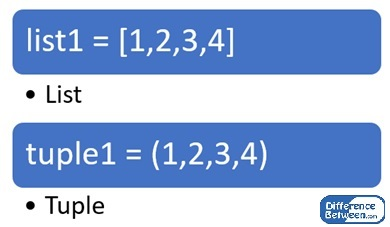
\includegraphics{Difference-Between-List-and-Tuple-fig-1-2.jpg}
\caption{At first glance list and tuples look very similar, but they are not\ldots{}}
\end{figure}

Like lists, tuples are containers of any type of object. Unlike lists though they are \emph{immutable} which means that once they have been created the content cannot be changed (i.e.~no append, insert or delete of the elements). Furthermore since they are immutable they can be used as dictionary keys (lists cannot).
To create a tuple the comma-separated list of items has to be enclosed in brackets, or the $\tt{tuple()}$ operator can be used.
Accessing tuple items is done in exactly the same way as lists.

\begin{tcolorbox}[breakable, size=fbox, boxrule=1pt, pad at break*=1mm, colback=cellbackground, colframe=cellborder]
\begin{Verbatim}[commandchars=\\\{\}]
\PY{n}{atuple} \PY{o}{=} \PY{p}{(}\PY{l+m+mi}{1}\PY{p}{,} \PY{l+m+mi}{2}\PY{p}{,} \PY{l+m+mi}{3}\PY{p}{)}
\PY{n+nb}{print} \PY{p}{(}\PY{l+s+s2}{\PYZdq{}}\PY{l+s+s2}{Length: }\PY{l+s+si}{\PYZob{}\PYZcb{}}\PY{l+s+s2}{\PYZdq{}}\PY{o}{.}\PY{n}{format}\PY{p}{(}\PY{n+nb}{len}\PY{p}{(}\PY{n}{atuple}\PY{p}{)}\PY{p}{)}\PY{p}{)}
\PY{n+nb}{print} \PY{p}{(}\PY{l+s+s2}{\PYZdq{}}\PY{l+s+s2}{First element: }\PY{l+s+si}{\PYZob{}\PYZcb{}}\PY{l+s+s2}{\PYZdq{}}\PY{o}{.}\PY{n}{format}\PY{p}{(}\PY{n}{atuple}\PY{p}{[}\PY{l+m+mi}{0}\PY{p}{]}\PY{p}{)}\PY{p}{)}
\PY{n+nb}{print} \PY{p}{(}\PY{l+s+s2}{\PYZdq{}}\PY{l+s+s2}{Last element: }\PY{l+s+si}{\PYZob{}\PYZcb{}}\PY{l+s+s2}{\PYZdq{}}\PY{o}{.}\PY{n}{format}\PY{p}{(}\PY{n}{atuple}\PY{p}{[}\PY{o}{\PYZhy{}}\PY{l+m+mi}{1}\PY{p}{]}\PY{p}{)}\PY{p}{)}

Length: 3
First element: 1
Last element: 3
\end{Verbatim}
\end{tcolorbox}

In the next snippet of code it is shown the so called unpacking which is another way to assign tuple values to variables.

\begin{tcolorbox}[breakable, size=fbox, boxrule=1pt, pad at break*=1mm, colback=cellbackground, colframe=cellborder]
\begin{Verbatim}[commandchars=\\\{\}]
\PY{n}{x}\PY{p}{,} \PY{n}{y}\PY{p}{,} \PY{n}{z} \PY{o}{=} \PY{p}{(}\PY{l+m+mi}{10}\PY{p}{,} \PY{l+m+mi}{5}\PY{p}{,} \PY{l+m+mi}{12}\PY{p}{)}
\PY{n+nb}{print} \PY{p}{(}\PY{l+s+s2}{\PYZdq{}}\PY{l+s+s2}{coord: x=}\PY{l+s+si}{\PYZob{}\PYZcb{}}\PY{l+s+s2}{ y=}\PY{l+s+si}{\PYZob{}\PYZcb{}}\PY{l+s+s2}{ z=}\PY{l+s+si}{\PYZob{}\PYZcb{}}\PY{l+s+s2}{\PYZdq{}}\PY{o}{.}\PY{n}{format}\PY{p}{(}\PY{n}{x}\PY{p}{,} \PY{n}{y}\PY{p}{,} \PY{n}{z}\PY{p}{)}\PY{p}{)}

coord: x=10 y=5 z=12
\end{Verbatim}
\end{tcolorbox}

If and ntuple has just one element don't forget the comma at the end otherwise it will be treated as a single number.

\begin{tcolorbox}[breakable, size=fbox, boxrule=1pt, pad at break*=1mm, colback=cellbackground, colframe=cellborder]
\begin{Verbatim}[commandchars=\\\{\}]
\PY{n}{tuple2} \PY{o}{=} \PY{p}{(}\PY{l+m+mi}{1}\PY{p}{,}\PY{p}{)}
\PY{n+nb}{print}\PY{p}{(}\PY{n+nb}{type}\PY{p}{(}\PY{n}{tuple2}\PY{p}{)}\PY{p}{)}
\PY{n}{tuple2} \PY{o}{=} \PY{p}{(}\PY{l+m+mi}{1}\PY{p}{)}
\PY{n+nb}{print}\PY{p}{(}\PY{n+nb}{type}\PY{p}{(}\PY{n}{tuple2}\PY{p}{)}\PY{p}{)}

<class 'tuple'>
<class 'int'>
\end{Verbatim}
\end{tcolorbox}

Since a tuple is immutable to add new elements it is necessary to create a new object:

\begin{tcolorbox}[breakable, size=fbox, boxrule=1pt, pad at break*=1mm, colback=cellbackground, colframe=cellborder]\begin{Verbatim}[commandchars=\\\{\}]
\PY{n}{tuple1} \PY{o}{=} \PY{p}{(}\PY{l+m+mi}{1}\PY{p}{,} \PY{l+m+mi}{2}\PY{p}{,} \PY{l+m+mi}{3}\PY{p}{)}
\PY{n}{tuple2} \PY{o}{=} \PY{n}{tuple1} \PY{o}{+} \PY{p}{(}\PY{l+m+mi}{4}\PY{p}{,} \PY{l+m+mi}{5}\PY{p}{)}
\PY{n+nb}{print}\PY{p}{(}\PY{n}{tuple2}\PY{p}{)}

(1,2,3,4,5)
\end{Verbatim}
\end{tcolorbox}

Finally, as already said tuples can be used as dictionary keys:

\begin{tcolorbox}[breakable, size=fbox, boxrule=1pt, pad at break*=1mm, colback=cellbackground, colframe=cellborder]\begin{Verbatim}[commandchars=\\\{\}]
\PY{n}{d} \PY{o}{=} \PY{p}{\PYZob{}}
   \PY{p}{(}\PY{l+s+s1}{\PYZsq{}}\PY{l+s+s1}{Finance}\PY{l+s+s1}{\PYZsq{}}\PY{p}{,} \PY{l+m+mi}{1}\PY{p}{)}\PY{p}{:} \PY{l+s+s1}{\PYZsq{}}\PY{l+s+s1}{Room 8}\PY{l+s+s1}{\PYZsq{}}\PY{p}{,}
    \PY{p}{(}\PY{l+s+s1}{\PYZsq{}}\PY{l+s+s1}{Finance}\PY{l+s+s1}{\PYZsq{}}\PY{p}{,} \PY{l+m+mi}{2}\PY{p}{)}\PY{p}{:} \PY{l+s+s1}{\PYZsq{}}\PY{l+s+s1}{Room 3}\PY{l+s+s1}{\PYZsq{}}\PY{p}{,}
    \PY{p}{(}\PY{l+s+s1}{\PYZsq{}}\PY{l+s+s1}{Math}\PY{l+s+s1}{\PYZsq{}}\PY{p}{,} \PY{l+m+mi}{1}\PY{p}{)}\PY{p}{:} \PY{l+s+s1}{\PYZsq{}}\PY{l+s+s1}{Room 6}\PY{l+s+s1}{\PYZsq{}}\PY{p}{,}
    \PY{p}{(}\PY{l+s+s1}{\PYZsq{}}\PY{l+s+s1}{Programming}\PY{l+s+s1}{\PYZsq{}}\PY{p}{,} \PY{l+m+mi}{1}\PY{p}{)}\PY{p}{:} \PY{l+s+s1}{\PYZsq{}}\PY{l+s+s1}{IT room}\PY{l+s+s1}{\PYZsq{}}
    \PY{p}{\PYZcb{}}
\end{Verbatim}
\end{tcolorbox}

Below the full list of tuple functions:
\begin{tcolorbox}[breakable, size=fbox, boxrule=1pt, pad at break*=1mm,colback=cellbackground, colframe=cellborder]
\begin{Verbatim}[commandchars=\\\{\}]
\PY{n+nb}{dir}\PY{p}{(}\PY{n+nb}{dict}\PY{p}{)}

[...
 'count',
 'index']
\end{Verbatim}
\end{tcolorbox}

%\clearpage
%\chapter{Date and Time}\label{introduction-to-python---lesson-1.6}

In this chapter we will take a little break and concentrate on a topic that it is not usually covered in this type of courses. However given its importance for financial computation the next paragraphs will be devoted to a close look up on the $\tt{datetime}$ module, whose utilities help in manipulating dates.

\section{Dates}\label{dates}

As said dates are not usually included in a standard \texttt{python} tutorial, however since they are pretty essential for finance we are going to cover this topic in some detail. In \texttt{python} the standard date class lives in the \texttt{datetime} module. We are also going to import \texttt{relativedelta} from the \texttt{dateutil} module, which allows to add/subtract days/months/years to dates, in other words to make operations on them.

In this first example the today's date is defined and with $\tt{relativedelta}$ two more date are created adding two months and three days to today.

\begin{tcolorbox}[breakable, size=fbox, boxrule=1pt, pad at break*=1mm,colback=cellbackground, colframe=cellborder]
\begin{Verbatim}[commandchars=\\\{\}]
\PY{k+kn}{from} \PY{n+nn}{datetime} \PY{k}{import} \PY{n}{date}\PY{p}{,} \PY{n}{datetime}
\PY{k+kn}{from} \PY{n+nn}{dateutil}\PY{n+nn}{.}\PY{n+nn}{relativedelta} \PY{k}{import} \PY{n}{relativedelta}

\PY{n}{date1} \PY{o}{=} \PY{n}{date}\PY{o}{.}\PY{n}{today}\PY{p}{(}\PY{p}{)}
\PY{n+nb}{print} \PY{p}{(}\PY{n}{date1}\PY{p}{)}
\PY{n}{date2} \PY{o}{=} \PY{n}{date}\PY{o}{.}\PY{n}{today}\PY{p}{(}\PY{p}{)} \PY{o}{+} \PY{n}{relativedelta}\PY{p}{(}\PY{n}{months}\PY{o}{=}\PY{l+m+mi}{2}\PY{p}{)}
\PY{n+nb}{print} \PY{p}{(}\PY{n}{date2}\PY{p}{)}
\PY{n}{date3} \PY{o}{=} \PY{n}{date}\PY{o}{.}\PY{n}{today}\PY{p}{(}\PY{p}{)} \PY{o}{\PYZhy{}} \PY{n}{relativedelta}\PY{p}{(}\PY{n}{days}\PY{o}{=}\PY{l+m+mi}{3}\PY{p}{)}
\PY{n+nb}{print} \PY{p}{(}\PY{n}{date3}\PY{p}{)}

2020-08-03
2020-10-03
2020-07-31
\end{Verbatim}
\end{tcolorbox}

Here instead another way of computing a new date is shown: in particular a one day delta is stored in a variable and today's date is moved by three days multiplying the defined delta by three.

\begin{tcolorbox}[breakable, size=fbox, boxrule=1pt, pad at break*=1mm,colback=cellbackground, colframe=cellborder]
\begin{Verbatim}[commandchars=\\\{\}]
\PY{n}{one\PYZus{}day} \PY{o}{=} \PY{n}{relativedelta}\PY{p}{(}\PY{n}{days}\PY{o}{=}\PY{l+m+mi}{1}\PY{p}{)}
\PY{n}{date}\PY{o}{.}\PY{n}{today}\PY{p}{(}\PY{p}{)} \PY{o}{\PYZhy{}} \PY{l+m+mi}{3} \PY{o}{*} \PY{n}{one\PYZus{}day}

datetime.date(2020, 7, 31)
\end{Verbatim}
\end{tcolorbox}

Next given two dates their difference is computed (and expressed in days).

\begin{tcolorbox}[breakable, size=fbox, boxrule=1pt, pad at break*=1mm,colback=cellbackground, colframe=cellborder]
\begin{Verbatim}[commandchars=\\\{\}]
\PY{n}{date1} \PY{o}{=} \PY{n}{date}\PY{p}{(}\PY{l+m+mi}{2019}\PY{p}{,} \PY{l+m+mi}{7}\PY{p}{,} \PY{l+m+mi}{2}\PY{p}{)}
\PY{n}{date2} \PY{o}{=} \PY{n}{date}\PY{p}{(}\PY{l+m+mi}{2019}\PY{p}{,} \PY{l+m+mi}{8}\PY{p}{,} \PY{l+m+mi}{16}\PY{p}{)}
\PY{p}{(}\PY{n}{date2} \PY{o}{\PYZhy{}} \PY{n}{date1}\PY{p}{)}\PY{o}{.}\PY{n}{days}

45
\end{Verbatim}
\end{tcolorbox}

Dates can be converted to and from strings and a large variety of formats can be specified in this conversions. The format is determined by a string in which each character starting with \% represent an element of the date, e.g. \%Y year, \%d day, \%s seconds, etc...

Below dates to string convertion:

\begin{tcolorbox}[breakable, size=fbox, boxrule=1pt, pad at break*=1mm,colback=cellbackground, colframe=cellborder]
\begin{Verbatim}[commandchars=\\\{\}]
\PY{n}{date1} \PY{o}{=} \PY{n}{date}\PY{p}{(}\PY{l+m+mi}{2019}\PY{p}{,} \PY{l+m+mi}{7}\PY{p}{,} \PY{l+m+mi}{2}\PY{p}{)}
\PY{n}{date1}\PY{o}{.}\PY{n}{strftime}\PY{p}{(}\PY{l+s+s2}{\PYZdq{}}\PY{l+s+s2}{\PYZpc{}}\PY{l+s+s2}{Y\PYZhy{}}\PY{l+s+s2}{\PYZpc{}}\PY{l+s+s2}{b\PYZhy{}}\PY{l+s+si}{\PYZpc{}d}\PY{l+s+s2}{ (}\PY{l+s+si}{\PYZpc{}a}\PY{l+s+s2}{)}\PY{l+s+s2}{\PYZdq{}}\PY{p}{)} \PY{c+c1}{\PYZsh{} dates can formatted in many ways}
                                \PY{c+c1}{\PYZsh{} check the docs for more details}

'2019-Jul-02 (Tue)'
\end{Verbatim}
\end{tcolorbox}

And here, strings are converted to datetime object:

\begin{tcolorbox}[breakable, size=fbox, boxrule=1pt, pad at break*=1mm,colback=cellbackground, colframe=cellborder]
\begin{Verbatim}[commandchars=\\\{\}]
\PY{c+c1}{\PYZsh{} a string can be convered to dates too}
\PY{n}{datetime}\PY{o}{.}\PY{n}{strptime}\PY{p}{(}\PY{l+s+s1}{\PYZsq{}}\PY{l+s+s1}{25 Aug 2019}\PY{l+s+s1}{\PYZsq{}}\PY{p}{,} \PY{l+s+s2}{\PYZdq{}}\PY{l+s+si}{\PYZpc{}d}\PY{l+s+s2}{ }\PY{l+s+s2}{\PYZpc{}}\PY{l+s+s2}{b }\PY{l+s+s2}{\PYZpc{}}\PY{l+s+s2}{Y}\PY{l+s+s2}{\PYZdq{}}\PY{p}{)}\PY{o}{.}\PY{n}{date}\PY{p}{(}\PY{p}{)}

datetime.date(2019, 8, 25)
\end{Verbatim}
\end{tcolorbox}

Finally a last example showing how to get the week-day from a date:

\begin{tcolorbox}[breakable, size=fbox, boxrule=1pt, pad at break*=1mm,colback=cellbackground, colframe=cellborder]
\begin{Verbatim}[commandchars=\\\{\}]
\PY{n}{date1}\PY{o}{.}\PY{n}{weekday}\PY{p}{(}\PY{p}{)} \PY{c+c1}{\PYZsh{} 0 = monday, ..., 6 = sunday}

1
\end{Verbatim}
\end{tcolorbox}

%\clearpage
%\chapter{Data Containers}\label{introduction-to-python---lesson-1.5}

In this chapter the container types available in $\tt{python}$ are reviewed.

\section{Lists}\label{lists}

A list in $\tt{python}$ is a container that is a \emph{mutable}, ordered sequence of elements. Each element or value that is inside of a list is called an \emph{item}. Each item can be accessed using square brackets notation (very important, list indexing is zero-based so the first element has index 0 actually). A list is considered mutable since you can add, remove or update the items in it. Ordered instead means that items are kept in the same order they have been added.
Lists can be created by enclosing in square brackets the comma-separated list of the items or using the $\tt{list()}$ operator.

\begin{tcolorbox}[breakable, size=fbox, boxrule=1pt, pad at break*=1mm, colback=cellbackground, colframe=cellborder]
  \begin{Verbatim}[commandchars=\\\{\}]
\PY{n}{mylist} \PY{o}{=} \PY{n+nb}{list}\PY{p}{([}\PY{l+m+mi}{21}\PY{p}{,} \PY{l+m+mi}{32}\PY{p}{,} \PY{l+m+mi}{15}\PY{p}{])}
\PY{n}{mylist} \PY{o}{=} \PY{p}{[}\PY{l+m+mi}{21}\PY{p}{,} \PY{l+m+mi}{32}\PY{p}{,} \PY{l+m+mi}{15}\PY{p}{]}
\PY{n+nb}{print}\PY{p}{(}\PY{n}{mylist}\PY{p}{)}
\PY{n+nb}{print} \PY{p}{(}\PY{n+nb}{type}\PY{p}{(}\PY{n}{mylist}\PY{p}{)}\PY{p}{)}

[21, 32, 15]
<class 'list'>
\end{Verbatim}
\end{tcolorbox}

\begin{tcolorbox}[breakable, size=fbox, boxrule=1pt, pad at break*=1mm, colback=cellbackground, colframe=cellborder]
\begin{Verbatim}[commandchars=\\\{\}]
\PY{n+nb}{print}\PY{p}{(}\PY{n}{mylist}\PY{p}{[}\PY{l+m+mi}{0}\PY{p}{]}\PY{p}{)}

21
\end{Verbatim}
\end{tcolorbox}

If you have a list of lists (i.e. a 2-dimensional list) you can use the square brackets multiple times to access the inner elements:
\begin{tcolorbox}[breakable, size=fbox, boxrule=1pt, pad at break*=1mm,colback=cellbackground, colframe=cellborder]
\begin{Verbatim}[commandchars=\\\{\}]                 
\PY{n}{alist} \PY{o}{=} \PY{p}{[}\PY{p}{[}\PY{l+m+mi}{1}\PY{p}{,}\PY{l+m+mi}{2}\PY{p}{]}\PY{p}{,} \PY{p}{[}\PY{l+m+mi}{3}\PY{p}{,}\PY{l+m+mi}{4}\PY{p}{]}\PY{p}{,} \PY{p}{[}\PY{l+m+mi}{5}\PY{p}{,}\PY{l+m+mi}{6}\PY{p}{]}\PY{p}{]}       
\PY{n+nb}{print} \PY{p}{(}\PY{n}{alist}\PY{p}{[}\PY{l+m+mi}{1}\PY{p}{]}\PY{p}{[}\PY{l+m+mi}{1}\PY{p}{]}\PY{p}{)} \PY{c+c1}{\PYZsh{} first [1] returns [3,4], second returns 4}                   
\end{Verbatim} 
\end{tcolorbox}  

The number of elements in a list is counted using the keyword \texttt{len()}:
\begin{tcolorbox}[breakable, size=fbox, boxrule=1pt, pad at break*=1mm, colback=cellbackground, colframe=cellborder]
\begin{Verbatim}[commandchars=\\\{\}]
\PY{n+nb}{print}\PY{p}{(}\PY{n+nb}{len}\PY{p}{(}\PY{n}{mylist}\PY{p}{)}\PY{p}{)}

3
\end{Verbatim}
\end{tcolorbox}

Looping on list items can be achieved in two ways: using directly the list or by index:

\begin{tcolorbox}[breakable, size=fbox, boxrule=1pt, pad at break*=1mm, colback=cellbackground, colframe=cellborder]
\begin{Verbatim}[commandchars=\\\{\}]
\PY{n+nb}{print} \PY{p}{(}\PY{l+s+s2}{\PYZdq{}}\PY{l+s+s2}{Loop using the list itself:}\PY{l+s+s2}{\PYZdq{}}\PY{p}{)}
\PY{k}{for} \PY{n}{i} \PY{o+ow}{in} \PY{n}{mylist}\PY{p}{:}
    \PY{n+nb}{print} \PY{p}{(}\PY{n}{i}\PY{p}{)}

\PY{n+nb}{print} \PY{p}{(}\PY{l+s+s2}{\PYZdq{}}\PY{l+s+s2}{Loop by index:}\PY{l+s+s2}{\PYZdq{}}\PY{p}{)}
\PY{k}{for} \PY{n}{i} \PY{o+ow}{in} \PY{n+nb}{range}\PY{p}{(}\PY{n+nb}{len}\PY{p}{(}\PY{n}{mylist}\PY{p}{)}\PY{p}{)}\PY{p}{:} \PY{c+c1}{\PYZsh{} len() returns the number of items in a list}
    \PY{n+nb}{print} \PY{p}{(}\PY{n}{mylist}\PY{p}{[}\PY{n}{i}\PY{p}{]}\PY{p}{)}

Loop using the list itself:
21
32
15

Loop by index:
21
32
15
\end{Verbatim}
\end{tcolorbox}

With the \texttt{enumerate} function is actually possible to do both at the same time since it returns two values, the index of the item and its value, so in the example below, \texttt{i} will take the item index values while \texttt{item} the item value itself:

\begin{tcolorbox}[breakable, size=fbox, boxrule=1pt, pad at break*=1mm, colback=cellbackground, colframe=cellborder]
\begin{Verbatim}[commandchars=\\\{\}]
\PY{k}{for} \PY{n}{i}\PY{p}{,} \PY{n}{item} \PY{o+ow}{in} \PY{n+nb}{enumerate}\PY{p}{(}\PY{n}{mylist}\PY{p}{)}\PY{p}{:}                        
    \PY{n+nb}{print} \PY{p}{(}\PY{n}{i}\PY{p}{,} \PY{n}{item}\PY{p}{)}

0 21
1 74
2 85
3 15
4 188
\end{Verbatim}
\end{tcolorbox}

Since a list is mutable we can dynamically change its items:

\begin{tcolorbox}[breakable, size=fbox, boxrule=1pt, pad at break*=1mm, colback=cellbackground, colframe=cellborder]
\begin{Verbatim}[commandchars=\\\{\}]
\PY{n}{mylist}\PY{p}{[}\PY{l+m+mi}{1}\PY{p}{]} \PY{o}{=} \PY{l+m+mi}{74} \PY{c+c1}{\PYZsh{} we can change list items since it\PYZsq{}s *mutable*}
\PY{n+nb}{print} \PY{p}{(}\PY{n}{mylist}\PY{p}{)}

[21, 74, 15]
\end{Verbatim}
\end{tcolorbox}

With \texttt{append} an item is added at the end, while with \texttt{insert} an item can be added in a specified position:

\begin{tcolorbox}[breakable, size=fbox, boxrule=1pt, pad at break*=1mm, colback=cellbackground, colframe=cellborder]
\begin{Verbatim}[commandchars=\\\{\}]
\PY{n}{mylist}\PY{o}{.}\PY{n}{append}\PY{p}{(}\PY{l+m+mi}{188}\PY{p}{)} \PY{c+c1}{\PYZsh{} append add an item at the end of the list}
\PY{n+nb}{print} \PY{p}{(}\PY{n}{mylist}\PY{p}{)}

[21, 74, 15, 188]

\PY{n}{mylist}\PY{o}{.}\PY{n}{insert}\PY{p}{(}\PY{l+m+mi}{2}\PY{p}{,} \PY{l+m+mi}{85}\PY{p}{)} \PY{c+c1}{\PYZsh{} insert an item in the desired position }
                     \PY{c+c1}{\PYZsh{} (2 in this example)}
\PY{n+nb}{print} \PY{p}{(}\PY{n}{mylist}\PY{p}{)}

[21, 74, 85, 15, 188]
\end{Verbatim}
\end{tcolorbox}

To append multiple values at once to a list a loop can be used but \texttt{python} offers a single line way of doing it: \texttt{[i*2 for i in range(10)]}. This syntax is called \emph{list comprehension}.

Accessing items outside the list range gives an error:

\begin{tcolorbox}[breakable, size=fbox, boxrule=1pt, pad at break*=1mm, colback=cellbackground, colframe=cellborder]
\begin{Verbatim}[commandchars=\\\{\}]
\PY{n}{mylist}\PY{p}{[}\PY{l+m+mi}{10}\PY{p}{]} \PY{c+c1}{\PYZsh{} error ! it doesn\PYZsq{}t exists, the list has only 3 }
           \PY{c+c1}{\PYZsh{} elements, so the last is item 2}

---------------------------------------------------------------------------

IndexError                                Traceback (most recent call last)

<ipython-input-36-ed1e5e6c3e46> in <module>
----> 1 mylist[10] \# error ! it doesn't exists, the list has only 3
      2           \# elements, so the last is item 2

IndexError: list index out of range
\end{Verbatim}
\end{tcolorbox}

Read carefully the error messages usually they are very explicative and can help a lot in \emph{debugging} (i.e. finding mistakes) in your programs.

There are two more nice features of $\tt{python}$ indexing:

\begin{itemize}
\item negative indices are like positive ones except that they starts from the last element;
\item \emph{slicing} which allows to specify a range of indices to select more items at once (if the first or last limits are missing slicing will start from the first or end with last index respectively).
\end{itemize}

\begin{tcolorbox}[breakable, size=fbox, boxrule=1pt, pad at break*=1mm, colback=cellbackground, colframe=cellborder]
\begin{Verbatim}[commandchars=\\\{\}]
\PY{n+nb}{print} \PY{p}{(}\PY{l+s+s2}{\PYZdq{}}\PY{l+s+s2}{negative index \PYZhy{}1 returns the last element:}\PY{l+s+s2}{\PYZdq{}}\PY{p}{,} \PY{n}{mylist}\PY{p}{[}\PY{o}{\PYZhy{}}\PY{l+m+mi}{1}\PY{p}{]}\PY{p}{)}
\PY{n+nb}{print} \PY{p}{(}\PY{l+s+s2}{\PYZdq{}}\PY{l+s+s2}{slice [1:3] returns items 1st and 2nd:}\PY{l+s+s2}{\PYZdq{}}\PY{p}{,} \PY{n}{mylist}\PY{p}{[}\PY{l+m+mi}{0}\PY{p}{:}\PY{l+m+mi}{3}\PY{p}{]}\PY{p}{)}
\PY{n+nb}{print} \PY{p}{(}\PY{l+s+s2}{\PYZdq{}}\PY{l+s+s2}{slice [:2] returns items 0th and 1st:}\PY{l+s+s2}{\PYZdq{}}\PY{p}{,} \PY{n}{mylist}\PY{p}{[}\PY{p}{:}\PY{l+m+mi}{2}\PY{p}{]}\PY{p}{)}
\PY{n+nb}{print} \PY{p}{(}\PY{l+s+s2}{\PYZdq{}}\PY{l+s+s2}{slice [2:] returns items between the 2nd and the last:}\PY{l+s+s2}{\PYZdq{}}\PY{p}{,} \PY{n}{mylist}\PY{p}{[}\PY{l+m+mi}{2}\PY{p}{:}\PY{p}{]}\PY{p}{)}

negative index -1 returns the last element: 188
slice [1:3] returns items 1st and 2nd: [21, 74, 85]
slice [:2] returns items 0th and 1st: [21, 74]
slice [2:] returns items between the 2nd and the last: [85, 15, 188]
\end{Verbatim}
\end{tcolorbox}

Needless to say that slicing with \texttt{[:]} returns the entire list.

It is worth mentioning that a list doesn't have to be populated
with the same kind of objects (list indices are instead always
integers).

\begin{tcolorbox}[breakable, size=fbox, boxrule=1pt, pad at break*=1mm, colback=cellbackground, colframe=cellborder]
\begin{Verbatim}[commandchars=\\\{\}]
\PY{n}{mixedlist} \PY{o}{=} \PY{p}{[}\PY{l+m+mi}{1}\PY{p}{,} \PY{l+m+mi}{2}\PY{p}{,} \PY{l+s+s2}{\PYZdq{}}\PY{l+s+s2}{b}\PY{l+s+s2}{\PYZdq{}}\PY{p}{,} \PY{n}{math}\PY{o}{.}\PY{n}{sqrt}\PY{p}{]}
\PY{n+nb}{print} \PY{p}{(}\PY{n}{mixedlist}\PY{p}{)}

[1, 2, 'b', <built-in function sqrt>]
\end{Verbatim}
\end{tcolorbox}

\begin{tcolorbox}[breakable, size=fbox, boxrule=1pt, pad at break*=1mm, colback=cellbackground, colframe=cellborder]
\begin{Verbatim}[commandchars=\\\{\}]
\PY{n+nb}{print} \PY{p}{(}\PY{n}{mixedlist}\PY{p}{[}\PY{l+s+s1}{\PYZsq{}}\PY{l+s+s1}{k}\PY{l+s+s1}{\PYZsq{}}\PY{p}{]}\PY{p}{)}

---------------------------------------------------------------------------

TypeError                                 Traceback (most recent call last)

<ipython-input-72-aea4c7f9789e> in <module>()
----> 1 print (mixedlist['k'])
    
TypeError: list indices must be integers or slices, not str
\end{Verbatim}
\end{tcolorbox}

A complete list of the commands available for a list can be shown with the $\tt{dir}$ statement:

\begin{tcolorbox}[breakable, size=fbox, boxrule=1pt, pad at break*=1mm,colback=cellbackground, colframe=cellborder]
\begin{Verbatim}[commandchars=\\\{\}]
\PY{n+nb}{dir}\PY{p}{(}\PY{n+nb}{list}\PY{p}{)}

[...
 'append',
 'clear',
 'copy',
 'count',
 'extend',
 'index',
 'insert',
 'pop',
 'remove',
 'reverse',
 'sort']
\end{Verbatim}
\end{tcolorbox}

Their meaning is pretty clear, so for example $\tt{sort}$ re-order the items according to a custom criteria or $\tt{index(item)}$ return the index of the specified item.

\section{Dictionaries}\label{dictionaries}

A we have seen lists are ordered collections of elements and as such we can say that map integers (the index of each item) to values (any kind of \texttt{python} object). \emph{Dictionaries} generalize such a concept being containers which map \emph{keys} (\textbf{almost} any kind of \texttt{python} object) to values (any kind of \texttt{python} object).

In our previous section we had:

\[ 0~(\textrm{0th item}) \rightarrow 21\]
\[ 1~(\textrm{1st item}) \rightarrow 74\]
\[ 2~(\textrm{2nd item}) \rightarrow 85\] \[ ... \]

With a dictionary we can have something like this:

\["apple" (\textrm{key}) \rightarrow 4 \]
\["banana" (\textrm{key}) \rightarrow 5 \]

As we will see dictionaries are very flexible and will be very useful to represent complex data structures.

Dictionaries can be created by enclosing in curly brackets the comma-separated list of key-value pairs (key and value are separated by a :), or using the $\tt{dict()}$ operator.
In lists we could access items by index, here we do it by key still using the square brackets. Trying to access not existing keys results in error, but we can check if a key exists with the \texttt{in} operator.
As before, if a dictionary contains other dictionaries or lists, the square brackets can be applied repeatedly to access the inner items.

\begin{tcolorbox}[breakable, size=fbox, boxrule=1pt, pad at break*=1mm, colback=cellbackground, colframe=cellborder]
\begin{Verbatim}[commandchars=\\\{\}]
\PY{n}{adict} \PY{o}{=} \PY{p}{\PYZob{}}\PY{l+s+s2}{\PYZdq{}}\PY{l+s+s2}{apple}\PY{l+s+s2}{\PYZdq{}}\PY{p}{:} \PY{l+m+mi}{4}\PY{p}{,} \PY{l+s+s2}{\PYZdq{}}\PY{l+s+s2}{banana}\PY{l+s+s2}{\PYZdq{}}\PY{p}{:} \PY{l+m+mi}{5}\PY{p}{\PYZcb{}}
\PY{n+nb}{print} \PY{p}{(}\PY{n}{adict}\PY{p}{[}\PY{l+s+s2}{\PYZdq{}}\PY{l+s+s2}{apple}\PY{l+s+s2}{\PYZdq{}}\PY{p}{]}\PY{p}{)}

4
\end{Verbatim}
\end{tcolorbox}

\begin{tcolorbox}[breakable, size=fbox, boxrule=1pt, pad at break*=1mm, colback=cellbackground, colframe=cellborder]
\begin{Verbatim}[commandchars=\\\{\}]
\PY{n}{adict}\PY{p}{[}\PY{l+s+s2}{\PYZdq{}}\PY{l+s+s2}{pear}\PY{l+s+s2}{\PYZdq{}}\PY{p}{]} \PY{c+c1}{\PYZsh{} error !}

---------------------------------------------------------------------------

KeyError                                  Traceback (most recent call last)

<ipython-input-41-9d051ebd10de> in <module>
----> 1 adict["pear"] \# error ! this key doesn't exists
    
KeyError: 'pear'
\end{Verbatim}
\end{tcolorbox}

\begin{tcolorbox}[breakable, size=fbox, boxrule=1pt, pad at break*=1mm, colback=cellbackground, colframe=cellborder]
\begin{Verbatim}[commandchars=\\\{\}]
\PY{l+s+s2}{\PYZdq{}}\PY{l+s+s2}{pear}\PY{l+s+s2}{\PYZdq{}} \PY{o+ow}{in} \PY{n}{adict} \PY{c+c1}{\PYZsh{} indeed}

False
\end{Verbatim}
\end{tcolorbox}

The items can be dynamically created or updated with the assignment \texttt{=} operator, while again \texttt{len()} returns the number of items in a dictionary.

\begin{tcolorbox}[breakable, size=fbox, boxrule=1pt, pad at break*=1mm, colback=cellbackground, colframe=cellborder]
\begin{Verbatim}[commandchars=\\\{\}]
\PY{n}{adict}\PY{p}{[}\PY{l+s+s2}{\PYZdq{}}\PY{l+s+s2}{banana}\PY{l+s+s2}{\PYZdq{}}\PY{p}{]} \PY{o}{=} \PY{l+m+mi}{2}
\PY{n}{adict}\PY{p}{[}\PY{l+s+s2}{\PYZdq{}}\PY{l+s+s2}{pear}\PY{l+s+s2}{\PYZdq{}}\PY{p}{]} \PY{o}{=} \PY{l+m+mi}{10}
\PY{n+nb}{print} \PY{p}{(}\PY{n+nb}{len}\PY{p}{(}\PY{n}{adict}\PY{p}{)}\PY{p}{)}
\PY{n+nb}{print} \PY{p}{(}\PY{n}{adict}\PY{p}{)}

3
\{'apple': 4, 'banana': 2, 'pear': 10\}
\end{Verbatim}
\end{tcolorbox}

Dictionaries can be made of more complicated types than simple string and integers:

\begin{tcolorbox}[breakable, size=fbox, boxrule=1pt, pad at break*=1mm, colback=cellbackground, colframe=cellborder]
\begin{Verbatim}[commandchars=\\\{\}]
\PY{n}{adict}\PY{p}{[}\PY{n}{math}\PY{o}{.}\PY{n}{log}\PY{p}{]} \PY{o}{=} \PY{n}{math}\PY{o}{.}\PY{n}{exp}
\end{Verbatim}
\end{tcolorbox}

Also dictionaries can be created with the \emph{comprehension} syntax: \texttt{\{i:v for i, v in enumerate(["a", "b", "c"])\}}.

Looping over dictionary items can be done by key, by value or by both: \texttt{.keys()} returns a list of keys, \texttt{.values()} returns a list of values and \texttt{.items()} a list of pairs key-value.

\begin{tcolorbox}[breakable, size=fbox, boxrule=1pt, pad at break*=1mm, colback=cellbackground, colframe=cellborder]
\begin{Verbatim}[commandchars=\\\{\}]
\PY{n+nb}{print} \PY{p}{(}\PY{l+s+s2}{\PYZdq{}}\PY{l+s+s2}{All keys: }\PY{l+s+s2}{\PYZdq{}}\PY{p}{,} \PY{n}{adict}\PY{o}{.}\PY{n}{keys}\PY{p}{(}\PY{p}{)}\PY{p}{)}
\PY{k}{for} \PY{n}{key} \PY{o+ow}{in} \PY{n}{adict}\PY{o}{.}\PY{n}{keys}\PY{p}{(}\PY{p}{)}\PY{p}{:}
    \PY{n+nb}{print} \PY{p}{(}\PY{n}{key}\PY{p}{)}

\PY{n+nb}{print} \PY{p}{(}\PY{l+s+s2}{\PYZdq{}}\PY{l+s+s2}{All values: }\PY{l+s+s2}{\PYZdq{}}\PY{p}{,} \PY{n}{adict}\PY{o}{.}\PY{n}{values}\PY{p}{(}\PY{p}{)}\PY{p}{)}
\PY{k}{for} \PY{n}{value} \PY{o+ow}{in} \PY{n}{adict}\PY{o}{.}\PY{n}{values}\PY{p}{(}\PY{p}{)}\PY{p}{:}
    \PY{n+nb}{print} \PY{p}{(}\PY{n}{value}\PY{p}{)}

\PY{n+nb}{print} \PY{p}{(}\PY{l+s+s2}{\PYZdq{}}\PY{l+s+s2}{All key\PYZhy{}value pairs: }\PY{l+s+s2}{\PYZdq{}}\PY{p}{,} \PY{n}{adict}\PY{o}{.}\PY{n}{items}\PY{p}{(}\PY{p}{)}\PY{p}{)}
\PY{k}{for} \PY{n}{key}\PY{p}{,} \PY{n}{value} \PY{o+ow}{in} \PY{n}{adict}\PY{o}{.}\PY{n}{items}\PY{p}{(}\PY{p}{)}\PY{p}{:}
    \PY{n+nb}{print} \PY{p}{(}\PY{n}{key}\PY{p}{,} \PY{n}{value}\PY{p}{)}

All keys:  dict\_keys(['apple', 'banana', 'pear', <built-in function log>])
apple
banana
pear
<built-in function log>

All values:  dict\_values([4, 2, 10, <built-in function exp>])
4
2
10
<built-in function exp>

All key-value pairs:  dict\_items([('apple', 4), ('banana', 2), ('pear', 10),
(<built-in function log>, <built-in function exp>)])
apple 4
banana 2
pear 10
<built-in function log> <built-in function exp>
\end{Verbatim}
\end{tcolorbox}

To merge two dictionaries the function \texttt{update()} can be used, while with \texttt{del} it is possible to remove a key-value pair.

\begin{tcolorbox}[breakable, size=fbox, boxrule=1pt, pad at break*=1mm, colback=cellbackground, colframe=cellborder]
\begin{Verbatim}[commandchars=\\\{\}]
\PY{k}{del} \PY{n}{adict}\PY{p}{[}\PY{n}{math}\PY{o}{.}\PY{n}{log}\PY{p}{]}
\PY{n}{seconddict} \PY{o}{=} \PY{p}{\PYZob{}}\PY{l+s+s2}{\PYZdq{}}\PY{l+s+s2}{watermelon}\PY{l+s+s2}{\PYZdq{}}\PY{p}{:} \PY{l+m+mi}{0}\PY{p}{,} \PY{l+s+s2}{\PYZdq{}}\PY{l+s+s2}{strawberry}\PY{l+s+s2}{\PYZdq{}}\PY{p}{:} \PY{l+m+mi}{1}\PY{p}{\PYZcb{}}
\PY{n}{adict}\PY{o}{.}\PY{n}{update}\PY{p}{(}\PY{n}{seconddict}\PY{p}{)}
\PY{n+nb}{print} \PY{p}{(}\PY{n}{adict}\PY{p}{)}

\{'apple': 4, 'banana': 2, 'pear': 10, 'watermelon': 0, 'strawberry': 1\}
\end{Verbatim}
\end{tcolorbox}

Again the complete list of dictionary functions can be shown with $\tt{dir}$:

\begin{tcolorbox}[breakable, size=fbox, boxrule=1pt, pad at break*=1mm,colback=cellbackground, colframe=cellborder]
\begin{Verbatim}[commandchars=\\\{\}]
\PY{n+nb}{dir}\PY{p}{(}\PY{n+nb}{dict}\PY{p}{)}

[...
 'clear',
 'copy',
 'fromkeys',
 'get',
 'items',
 'keys',
 'pop',
 'popitem',
 'setdefault',
 'update',
 'values']
\end{Verbatim}
\end{tcolorbox}

\section{Tuples}\label{tuples}

Tuples create a bit of confusion for beginners because they are very similar to lists but they have some subtle conceptual differences.
Nonetheless, tuples do appear when programming in $\tt{python}$ so it's important to know about them.

\begin{figure}[hb]
\centering
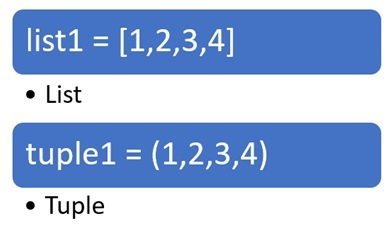
\includegraphics[width=0.5\textwidth]{figures/Difference-Between-List-and-Tuple-fig-1-2.jpg}
\caption{At first glance list and tuples look very similar, but they are not\ldots{}}
\end{figure}

Like lists, tuples are containers of any type of object. Unlike lists though they are \emph{immutable} which means that once they have been created the content cannot be changed (i.e.~no append, insert or delete of the elements). Furthermore since they are immutable they can be used as dictionary keys (lists cannot).
To create a tuple the comma-separated list of items has to be enclosed in brackets, or the $\tt{tuple()}$ operator can be used.
Accessing tuple items is done in exactly the same way as lists.

\begin{tcolorbox}[breakable, size=fbox, boxrule=1pt, pad at break*=1mm, colback=cellbackground, colframe=cellborder]
\begin{Verbatim}[commandchars=\\\{\}]
\PY{n}{atuple} \PY{o}{=} \PY{p}{(}\PY{l+m+mi}{1}\PY{p}{,} \PY{l+m+mi}{2}\PY{p}{,} \PY{l+m+mi}{3}\PY{p}{)}
\PY{n+nb}{print} \PY{p}{(}\PY{l+s+s2}{\PYZdq{}}\PY{l+s+s2}{Length: }\PY{l+s+si}{\PYZob{}\PYZcb{}}\PY{l+s+s2}{\PYZdq{}}\PY{o}{.}\PY{n}{format}\PY{p}{(}\PY{n+nb}{len}\PY{p}{(}\PY{n}{atuple}\PY{p}{)}\PY{p}{)}\PY{p}{)}
\PY{n+nb}{print} \PY{p}{(}\PY{l+s+s2}{\PYZdq{}}\PY{l+s+s2}{First element: }\PY{l+s+si}{\PYZob{}\PYZcb{}}\PY{l+s+s2}{\PYZdq{}}\PY{o}{.}\PY{n}{format}\PY{p}{(}\PY{n}{atuple}\PY{p}{[}\PY{l+m+mi}{0}\PY{p}{]}\PY{p}{)}\PY{p}{)}
\PY{n+nb}{print} \PY{p}{(}\PY{l+s+s2}{\PYZdq{}}\PY{l+s+s2}{Last element: }\PY{l+s+si}{\PYZob{}\PYZcb{}}\PY{l+s+s2}{\PYZdq{}}\PY{o}{.}\PY{n}{format}\PY{p}{(}\PY{n}{atuple}\PY{p}{[}\PY{o}{\PYZhy{}}\PY{l+m+mi}{1}\PY{p}{]}\PY{p}{)}\PY{p}{)}

Length: 3
First element: 1
Last element: 3
\end{Verbatim}
\end{tcolorbox}

In the next snippet of code it is shown the so called unpacking which is another way to assign tuple values to variables.

\begin{tcolorbox}[breakable, size=fbox, boxrule=1pt, pad at break*=1mm, colback=cellbackground, colframe=cellborder]
\begin{Verbatim}[commandchars=\\\{\}]
\PY{n}{x}\PY{p}{,} \PY{n}{y}\PY{p}{,} \PY{n}{z} \PY{o}{=} \PY{p}{(}\PY{l+m+mi}{10}\PY{p}{,} \PY{l+m+mi}{5}\PY{p}{,} \PY{l+m+mi}{12}\PY{p}{)}
\PY{n+nb}{print} \PY{p}{(}\PY{l+s+s2}{\PYZdq{}}\PY{l+s+s2}{coord: x=}\PY{l+s+si}{\PYZob{}\PYZcb{}}\PY{l+s+s2}{ y=}\PY{l+s+si}{\PYZob{}\PYZcb{}}\PY{l+s+s2}{ z=}\PY{l+s+si}{\PYZob{}\PYZcb{}}\PY{l+s+s2}{\PYZdq{}}\PY{o}{.}\PY{n}{format}\PY{p}{(}\PY{n}{x}\PY{p}{,} \PY{n}{y}\PY{p}{,} \PY{n}{z}\PY{p}{)}\PY{p}{)}

coord: x=10 y=5 z=12
\end{Verbatim}
\end{tcolorbox}

If an ntuple has just one element don't forget the comma at the end otherwise it will be treated as a single number.

\begin{tcolorbox}[breakable, size=fbox, boxrule=1pt, pad at break*=1mm, colback=cellbackground, colframe=cellborder]
\begin{Verbatim}[commandchars=\\\{\}]
\PY{n}{tuple2} \PY{o}{=} \PY{p}{(}\PY{l+m+mi}{1}\PY{p}{,}\PY{p}{)}
\PY{n+nb}{print}\PY{p}{(}\PY{n+nb}{type}\PY{p}{(}\PY{n}{tuple2}\PY{p}{)}\PY{p}{)}
\PY{n}{tuple2} \PY{o}{=} \PY{p}{(}\PY{l+m+mi}{1}\PY{p}{)}
\PY{n+nb}{print}\PY{p}{(}\PY{n+nb}{type}\PY{p}{(}\PY{n}{tuple2}\PY{p}{)}\PY{p}{)}

<class 'tuple'>
<class 'int'>
\end{Verbatim}
\end{tcolorbox}

Since a tuple is immutable to add new elements it is necessary to create a new object:

\begin{tcolorbox}[breakable, size=fbox, boxrule=1pt, pad at break*=1mm, colback=cellbackground, colframe=cellborder]\begin{Verbatim}[commandchars=\\\{\}]
\PY{n}{tuple1} \PY{o}{=} \PY{p}{(}\PY{l+m+mi}{1}\PY{p}{,} \PY{l+m+mi}{2}\PY{p}{,} \PY{l+m+mi}{3}\PY{p}{)}
\PY{n}{tuple2} \PY{o}{=} \PY{n}{tuple1} \PY{o}{+} \PY{p}{(}\PY{l+m+mi}{4}\PY{p}{,} \PY{l+m+mi}{5}\PY{p}{)}
\PY{n+nb}{print}\PY{p}{(}\PY{n}{tuple2}\PY{p}{)}

(1,2,3,4,5)
\end{Verbatim}
\end{tcolorbox}

Finally, as already said tuples can be used as dictionary keys:

\begin{tcolorbox}[breakable, size=fbox, boxrule=1pt, pad at break*=1mm, colback=cellbackground, colframe=cellborder]\begin{Verbatim}[commandchars=\\\{\}]
\PY{n}{d} \PY{o}{=} \PY{p}{\PYZob{}}
   \PY{p}{(}\PY{l+s+s1}{\PYZsq{}}\PY{l+s+s1}{Finance}\PY{l+s+s1}{\PYZsq{}}\PY{p}{,} \PY{l+m+mi}{1}\PY{p}{)}\PY{p}{:} \PY{l+s+s1}{\PYZsq{}}\PY{l+s+s1}{Room 8}\PY{l+s+s1}{\PYZsq{}}\PY{p}{,}
    \PY{p}{(}\PY{l+s+s1}{\PYZsq{}}\PY{l+s+s1}{Finance}\PY{l+s+s1}{\PYZsq{}}\PY{p}{,} \PY{l+m+mi}{2}\PY{p}{)}\PY{p}{:} \PY{l+s+s1}{\PYZsq{}}\PY{l+s+s1}{Room 3}\PY{l+s+s1}{\PYZsq{}}\PY{p}{,}
    \PY{p}{(}\PY{l+s+s1}{\PYZsq{}}\PY{l+s+s1}{Math}\PY{l+s+s1}{\PYZsq{}}\PY{p}{,} \PY{l+m+mi}{1}\PY{p}{)}\PY{p}{:} \PY{l+s+s1}{\PYZsq{}}\PY{l+s+s1}{Room 6}\PY{l+s+s1}{\PYZsq{}}\PY{p}{,}
    \PY{p}{(}\PY{l+s+s1}{\PYZsq{}}\PY{l+s+s1}{Programming}\PY{l+s+s1}{\PYZsq{}}\PY{p}{,} \PY{l+m+mi}{1}\PY{p}{)}\PY{p}{:} \PY{l+s+s1}{\PYZsq{}}\PY{l+s+s1}{IT room}\PY{l+s+s1}{\PYZsq{}}
    \PY{p}{\PYZcb{}}
\end{Verbatim}
\end{tcolorbox}

Below the full list of tuple functions:
\begin{tcolorbox}[breakable, size=fbox, boxrule=1pt, pad at break*=1mm,colback=cellbackground, colframe=cellborder]
\begin{Verbatim}[commandchars=\\\{\}]
\PY{n+nb}{dir}\PY{p}{(}\PY{n+nb}{dict}\PY{p}{)}

[...
 'count',
 'index']
\end{Verbatim}
\end{tcolorbox}

%\begin{thebibliography}{9}
%  %\bibitem{survey2019} StackOverflow \emph{The TEXbook}, Addison-Wesley, Reading,Massachusetts, second edition, 1984,
%\bibitem{survey2019} \emph{https://insights.stackoverflow.com/survey/2019}, Stack Overflow, 2019 [Online]
%\bibitem{python_versions} \emph{https://www.python.org/downloads/}, \texttt{python.org} [Online]
%\bibitem{learn_python} \emph{https://www.learnpython.org/it/}, \texttt{learnpython.org} [Online]
%\bibitem{freecamp} \emph{https://www.youtube.com/watch?v=8DvywoWv6fI}, \textt{freeCodeCamp.org} [Online]
%\bibitem{modules} \emph{https://docs.python.org/3/py-modindex.html}, Complete list of \texttt{python} modules [Online]
%\end{thebibliography}
%

%\clearpage
%\chapter{Data Manipulation and Its Representation}

In this chapter a closer look two a couple more of modules is given. These modules will result to be very useful in managing financial data and to report result of our analysis.

\section{Getting Data}\label{getting-data}

The first step of any analysis is usually the one that involves selection and manipulation of data we want to process. Data sources can be various (eg. website, figures, twitter messages, CSV or Excel files\ldots{}) and partially reflect its nature which can range from \emph{unstructured} data (whitout any inherent structure, e.g.~social media data) to completely \emph{structured} data (where the data model is defined and usually there is no error associated, e.g.~stock trading data).

Our primary goal, before start processing data, is to collect and store the information in a suitable data structure. \texttt{Python} provides a very useful module, called \texttt{pandas}, which allows to collect and save data in \emph{dataframe} objects that can be later on manipulated for analysis purposes.

Looking at \texttt{pandas} manual dataframe are defined as multi-dimensional, size-mutable, potentially heterogenous, tabular data structure with labeled axes (rows and columns), in much simpler words it is a table whose structure can be modified.
It presents data in a way that is suitable for data analysis, contains multiple methods for convenient data filtering and in addition has a lot of utilities to load and save data pretty easly.

Dataframes can be created by:
\begin{itemize}
\item importing data from file;
\item creating by hand data and then filling the dataframe.
\end{itemize}


\begin{tcolorbox}[breakable, size=fbox, boxrule=1pt, pad at break*=1mm,colback=cellbackground, colframe=cellborder]
\begin{Verbatim}[commandchars=\\\{\}]
\PY{k+kn}{import} \PY{n+nn}{pandas} \PY{k}{as} \PY{n+nn}{pd}

\PY{c+c1}{\PYZsh{} reading from file}
\PY{n}{df1} \PY{o}{=} \PY{n}{pd}\PY{o}{.}\PY{n}{read\PYZus{}excel}\PY{p}{(}\PY{l+s+s1}{\PYZsq{}}\PY{l+s+s1}{sample.xlsx}\PY{l+s+s1}{\PYZsq{}}\PY{p}{)} \PY{c+c1}{\PYZsh{} Excel file}
\PY{n}{df2} \PY{o}{=} \PY{n}{pd}\PY{o}{.}\PY{n}{read\PYZus{}csv}\PY{p}{(}\PY{l+s+s1}{\PYZsq{}}\PY{l+s+s1}{sample.csv}\PY{l+s+s1}{\PYZsq{}}\PY{p}{)} \PY{c+c1}{\PYZsh{} Comma Separeted file}

\PY{n}{df1}\PY{o}{.}\PY{n}{head}\PY{p}{(}\PY{l+m+mi}{11}\PY{p}{)} \PY{c+c1}{\PYZsh{} show just few rows at the beginning}

         Date       Price      Volume
0  2000-07-30  100.000000  191.811275
1  2000-07-31  129.216267  190.897541
2  2000-08-01  147.605516  197.476379
3  2000-08-02  107.282251  199.660061
4  2000-08-03  106.036826  200.840459
5  2000-08-04  118.872757  197.130212
6  2000-08-05  101.904544  204.552521
7  2000-08-06  106.392901  198.160030
8  2000-08-06  106.392901  191.125969
9  2000-08-06  106.392901  196.719061
10 2000-08-06  106.392901  196.759837
\end{Verbatim}
\end{tcolorbox}

\begin{tcolorbox}[breakable, size=fbox, boxrule=1pt, pad at break*=1mm,colback=cellbackground, colframe=cellborder]
\begin{Verbatim}[commandchars=\\\{\}]
\PY{c+c1}{\PYZsh{} creating some data in a dictionary}
\PY{n}{d} \PY{o}{=} \PY{p}{\PYZob{}}\PY{l+s+s2}{\PYZdq{}}\PY{l+s+s2}{Nome}\PY{l+s+s2}{\PYZdq{}}\PY{p}{:}\PY{p}{[}\PY{l+s+s2}{\PYZdq{}}\PY{l+s+s2}{Elisa}\PY{l+s+s2}{\PYZdq{}}\PY{p}{,} \PY{l+s+s2}{\PYZdq{}}\PY{l+s+s2}{Roberto}\PY{l+s+s2}{\PYZdq{}}\PY{p}{,} \PY{l+s+s2}{\PYZdq{}}\PY{l+s+s2}{Ciccio}\PY{l+s+s2}{\PYZdq{}}\PY{p}{,} \PY{l+s+s2}{\PYZdq{}}\PY{l+s+s2}{Topolino}\PY{l+s+s2}{\PYZdq{}}\PY{p}{,} \PY{l+s+s2}{\PYZdq{}}\PY{l+s+s2}{Gigi}\PY{l+s+s2}{\PYZdq{}}\PY{p}{]}\PY{p}{,}
     \PY{l+s+s2}{\PYZdq{}}\PY{l+s+s2}{Età}\PY{l+s+s2}{\PYZdq{}}\PY{p}{:}\PY{p}{[}\PY{l+m+mi}{1}\PY{p}{,} \PY{l+m+mi}{27}\PY{p}{,} \PY{l+m+mi}{25}\PY{p}{,} \PY{l+m+mi}{24}\PY{p}{,} \PY{l+m+mi}{31}\PY{p}{]}\PY{p}{,}
     \PY{l+s+s2}{\PYZdq{}}\PY{l+s+s2}{Punteggio}\PY{l+s+s2}{\PYZdq{}}\PY{p}{:}\PY{p}{[}\PY{l+m+mi}{100}\PY{p}{,} \PY{l+m+mi}{120}\PY{p}{,} \PY{l+m+mi}{95}\PY{p}{,} \PY{l+m+mi}{1300}\PY{p}{,} \PY{l+m+mi}{101}\PY{p}{]}\PY{p}{\PYZcb{}}

\PY{c+c1}{\PYZsh{} filling the dataframe}
\PY{n}{df} \PY{o}{=} \PY{n}{pd}\PY{o}{.}\PY{n}{DataFrame}\PY{p}{(}\PY{n}{d}\PY{p}{)}
\PY{n}{df}\PY{o}{.}\PY{n}{head}\PY{p}{(}\PY{p}{)}

       Nome  Età  Punteggio
0     Elisa    1        100
1   Roberto   27        120
2    Ciccio   25         95
3  Topolino   24       1300
4      Gigi   31        101
\end{Verbatim}
\end{tcolorbox}

Of course with \texttt{pandas} it is possible to perform a large number of operations on a dataframe. For example it is possible to add a column as a result of an operation on other columns. Looking back at the \texttt{df1} dataframe it is possible to add a column with the daily variation of the price.

\begin{tcolorbox}[breakable, size=fbox, boxrule=1pt, pad at break*=1mm,colback=cellbackground, colframe=cellborder]
\begin{Verbatim}[commandchars=\\\{\}]
\PY{k+kn}{import} \PY{n+nn}{numpy} \PY{k}{as} \PY{n+nn}{np}

\PY{c+c1}{\PYZsh{} first let\PYZsq{}s add an empty column}
\PY{n}{df1}\PY{p}{[}\PY{l+s+s1}{\PYZsq{}}\PY{l+s+s1}{Variation}\PY{l+s+s1}{\PYZsq{}}\PY{p}{]} \PY{o}{=} \PY{n}{np}\PY{o}{.}\PY{n}{nan} \PY{c+c1}{\PYZsh{} nan stands for not a number}

\PY{c+c1}{\PYZsh{} loop on the Price column, compute the variation and fill the column}
\PY{c+c1}{\PYZsh{} len returns the number of rows of a dataframe}
\PY{k}{for} \PY{n}{i} \PY{o+ow}{in} \PY{n+nb}{range}\PY{p}{(}\PY{l+m+mi}{1}\PY{p}{,} \PY{n+nb}{len}\PY{p}{(}\PY{n}{df1}\PY{p}{)}\PY{p}{)}\PY{p}{:}
    \PY{c+c1}{\PYZsh{} select the ith row and fill \PYZdq{}Variation\PYZdq{}}
    \PY{c+c1}{\PYZsh{} loc takes as inputs row and colum\PYZhy{}name}
    \PY{n}{df1}\PY{o}{.}\PY{n}{loc}\PY{p}{[}\PY{n}{i}\PY{p}{,} \PY{l+s+s2}{\PYZdq{}}\PY{l+s+s2}{Variation}\PY{l+s+s2}{\PYZdq{}}\PY{p}{]} \PY{o}{=} \PY{p}{(}\PY{n}{df1}\PY{o}{.}\PY{n}{loc}\PY{p}{[}\PY{n}{i}\PY{p}{,} \PY{l+s+s2}{\PYZdq{}}\PY{l+s+s2}{Price}\PY{l+s+s2}{\PYZdq{}}\PY{p}{]} \PY{o}{\PYZhy{}} \PY{n}{df1}\PY{o}{.}\PY{n}{loc}\PY{p}{[}\PY{n}{i}\PY{o}{\PYZhy{}}\PY{l+m+mi}{1}\PY{p}{,} \PY{l+s+s2}{\PYZdq{}}\PY{l+s+s2}{Price}\PY{l+s+s2}{\PYZdq{}}\PY{p}{]}\PY{p}{)} \PY{o}{/}
                      \PY{n}{df1}\PY{o}{.}\PY{n}{loc}\PY{p}{[}\PY{n}{i}\PY{o}{\PYZhy{}}\PY{l+m+mi}{1}\PY{p}{,} \PY{l+s+s2}{\PYZdq{}}\PY{l+s+s2}{Price}\PY{l+s+s2}{\PYZdq{}}\PY{p}{]}

\PY{n}{df1}\PY{o}{.}\PY{n}{head}\PY{p}{(}\PY{p}{)}

        Date       Price      Volume  Variation
0 2000-07-30  100.000000  191.811275        NaN
1 2000-07-31  129.216267  190.897541   0.292163
2 2000-08-01  147.605516  197.476379   0.142314
3 2000-08-02  107.282251  199.660061  -0.273183
4 2000-08-03  106.036826  200.840459  -0.011609
\end{Verbatim}
\end{tcolorbox}

Of course the first ``variation'' value is NaN since there is no previous price to compare with.

\subsection{Manage Data}\label{manage-data}

Once we have created our dataframe we may want to preliminarly process data to perform very common operations like:

\begin{itemize}
\item remove unwanted observations or outliers;
\item handle missing data;
\item filter, sort and clean data.
\end{itemize}

\subsection{Unwanted observations and outliers}

\subsubsection{Duplicates}

It may happen that our data has duplicates (e.g.~those can arise when combining two datasets), or the dataset contains irrelvant fields for the specific study we are carrying on. To find and remove duplicates \texttt{pandas} has convenient methods:

\begin{tcolorbox}[breakable, size=fbox, boxrule=1pt, pad at break*=1mm,colback=cellbackground, colframe=cellborder]
\begin{Verbatim}[commandchars=\\\{\}]
\PY{c+c1}{\PYZsh{} find duplicates based on all columns}
\PY{c+c1}{\PYZsh{} and show just the first 15 results  }
\PY{c+c1}{\PYZsh{}print (df1.duplicated()[:15]) }

\PY{c+c1}{\PYZsh{} find duplicates based on\PYZsq{}Price\PYZsq{}}
\PY{c+c1}{\PYZsh{} and show just the first 15 results}
\PY{n+nb}{print} \PY{p}{(}\PY{n}{df1}\PY{o}{.}\PY{n}{duplicated}\PY{p}{(}\PY{n}{subset}\PY{o}{=}\PY{p}{[}\PY{l+s+s1}{\PYZsq{}}\PY{l+s+s1}{Price}\PY{l+s+s1}{\PYZsq{}}\PY{p}{]}\PY{p}{)}\PY{p}{[}\PY{p}{:}\PY{l+m+mi}{15}\PY{p}{]} \PY{p}{)}

0     False
1     False
2     False
3     False
4     False
5     False
6     False
7     False
8      True
9      True
10     True
11    False
12    False
13    False
14    False
dtype: bool
\end{Verbatim}
\end{tcolorbox}












\begin{tcolorbox}[breakable, size=fbox, boxrule=1pt, pad at break*=1mm,colback=cellbackground, colframe=cellborder]
\begin{Verbatim}[commandchars=\\\{\}]
\PY{n+nb}{print} \PY{p}{(}\PY{l+s+s2}{\PYZdq{}}\PY{l+s+s2}{Initial number of rows: }\PY{l+s+si}{\PYZob{}\PYZcb{}}\PY{l+s+s2}{\PYZdq{}}\PY{o}{.}\PY{n}{format}\PY{p}{(}\PY{n+nb}{len}\PY{p}{(}\PY{n}{df1}\PY{p}{)}\PY{p}{)}\PY{p}{)} 

\PY{c+c1}{\PYZsh{} remove duplicates}
\PY{c+c1}{\PYZsh{} where the second argument can be `first`, `last` }
\PY{c+c1}{\PYZsh{} or `False` (consider all of the same values as duplicates).}
\PY{n}{df1} \PY{o}{=} \PY{n}{df1}\PY{o}{.}\PY{n}{drop\PYZus{}duplicates}\PY{p}{(}\PY{n}{subset}\PY{o}{=}\PY{l+s+s1}{\PYZsq{}}\PY{l+s+s1}{Price}\PY{l+s+s1}{\PYZsq{}}\PY{p}{,} \PY{n}{keep}\PY{o}{=}\PY{l+s+s1}{\PYZsq{}}\PY{l+s+s1}{first}\PY{l+s+s1}{\PYZsq{}}\PY{p}{)}

\PY{n+nb}{print} \PY{p}{(}\PY{l+s+s2}{\PYZdq{}}\PY{l+s+s2}{Number of columns after drop: }\PY{l+s+si}{\PYZob{}\PYZcb{}}\PY{l+s+s2}{\PYZdq{}}\PY{o}{.}\PY{n}{format}\PY{p}{(}\PY{n+nb}{len}\PY{p}{(}\PY{n}{df1}\PY{p}{)}\PY{p}{)}\PY{p}{)}

Initial number of rows: 734
Number of columns after drop: 729
\end{Verbatim}
\end{tcolorbox}

If we would like to drop irrilevant columns for our analysis it is enough to:

\begin{tcolorbox}[breakable, size=fbox, boxrule=1pt, pad at break*=1mm,colback=cellbackground, colframe=cellborder]
\begin{Verbatim}[commandchars=\\\{\}]
\PY{n}{df2} \PY{o}{=} \PY{n}{df2}\PY{o}{.}\PY{n}{drop}\PY{p}{(}\PY{n}{columns}\PY{o}{=}\PY{p}{[}\PY{l+s+s1}{\PYZsq{}}\PY{l+s+s1}{Volume}\PY{l+s+s1}{\PYZsq{}}\PY{p}{]}\PY{p}{)}
\PY{n}{df2}\PY{o}{.}\PY{n}{head}\PY{p}{(}\PY{p}{)}

         Date       Price
0  2000-07-30  100.000000
1  2000-07-31  129.216267
2  2000-08-01  147.605516
3  2000-08-02  107.282251
4  2000-08-03  106.036826
\end{Verbatim}
\end{tcolorbox}
        
If instead we just want to remove few rows we can select them by index:

\begin{tcolorbox}[breakable, size=fbox, boxrule=1pt, pad at break*=1mm,colback=cellbackground, colframe=cellborder]
\begin{Verbatim}[commandchars=\\\{\}]
\PY{c+c1}{\PYZsh{} we remove row 0th and 2nd}
\PY{c+c1}{\PYZsh{} axis=0 means use the index column}
\PY{n}{df2} \PY{o}{=} \PY{n}{df2}\PY{o}{.}\PY{n}{drop}\PY{p}{(}\PY{p}{[}\PY{l+m+mi}{0}\PY{p}{,} \PY{l+m+mi}{2}\PY{p}{]}\PY{p}{,} \PY{n}{axis}\PY{o}{=}\PY{l+m+mi}{0}\PY{p}{)}
\PY{n}{df2}\PY{o}{.}\PY{n}{head}\PY{p}{(}\PY{p}{)}

         Date       Price
1  2000-07-31  129.216267
3  2000-08-02  107.282251
4  2000-08-03  106.036826
5  2000-08-04  118.872757
6  2000-08-05  101.904544
\end{Verbatim}
\end{tcolorbox}
        
Changing the column that act as index we can select the rows also by other attributes:

\begin{tcolorbox}[breakable, size=fbox, boxrule=1pt, pad at break*=1mm,colback=cellbackground, colframe=cellborder]
\begin{Verbatim}[commandchars=\\\{\}]
\PY{c+c1}{\PYZsh{} tell pandas to use Date as index column}
\PY{n}{df2} \PY{o}{=} \PY{n}{df2}\PY{o}{.}\PY{n}{set\PYZus{}index}\PY{p}{(}\PY{l+s+s1}{\PYZsq{}}\PY{l+s+s1}{Date}\PY{l+s+s1}{\PYZsq{}}\PY{p}{)}

\PY{c+c1}{\PYZsh{} select row to remove by date at this point}
\PY{n}{df2} \PY{o}{=} \PY{n}{df2}\PY{o}{.}\PY{n}{drop}\PY{p}{(}\PY{p}{[}\PY{l+s+s2}{\PYZdq{}}\PY{l+s+s2}{2000\PYZhy{}07\PYZhy{}31}\PY{l+s+s2}{\PYZdq{}}\PY{p}{]}\PY{p}{,} \PY{n}{axis}\PY{o}{=}\PY{l+m+mi}{0}\PY{p}{)}

\PY{n}{df2}\PY{o}{.}\PY{n}{head}\PY{p}{(}\PY{p}{)}

Date        Price
2000-08-02  107.282251
2000-08-03  106.036826
2000-08-04  118.872757
2000-08-05  101.904544
2000-08-06  106.392901
\end{Verbatim}
\end{tcolorbox}
        
\subsubsection{Outliers}\label{outliers}

An outlier is an observation that lies outside the overall pattern of a distribution. Common causes can be human, measurement or experimental errors. Outliers must be handled carefully and we should remove them cautiously, \emph{outliers are innocent until proven guilty}. We may have removed the most interesting part of our dataset !

The core statistics about a particular column can be studied by the \texttt{describe()} method which returns the following information:
\begin{itemize}
\item for numeric columns: the value count, mean, standard deviation, minimum, maximum and 25th, 50th and 75h quantiles for the data in a column;
\item for string columns: the number of unique entries, the most frequent occurring value (\emph{top}), and the number of times the top value occurs (\emph{freq}).
\end{itemize}

\begin{tcolorbox}[breakable, size=fbox, boxrule=1pt, pad at break*=1mm,colback=cellbackground, colframe=cellborder]
\begin{Verbatim}[commandchars=\\\{\}]
\PY{n}{df1}\PY{o}{.}\PY{n}{describe}\PY{p}{(}\PY{p}{)}

              Price      Volume   Variation
count    728.000000  729.000000  724.000000
mean     120.898678  200.355900    0.146330
std      490.493411    4.970745    3.637952
min        0.878873  186.430551   -0.995284
25\%       14.809934  196.998603   -0.119423
50\%       61.325699  200.221125   -0.005549
75\%      164.021813  203.580691    0.121290
max    13000.000000  215.140868   97.756432
\end{Verbatim}
\end{tcolorbox}
        
Looking at mean and std and comparing it with min and max values we could find a range outside of which we may have outliers. For example 13000.0 is several standard deviation away the mean which may indicate that it is not a good value.

Another way to spot outliers is to plot column distributions and again \texttt{pandas} comes to help us:

\begin{tcolorbox}[breakable, size=fbox, boxrule=1pt, pad at break*=1mm,colback=cellbackground, colframe=cellborder]
\begin{Verbatim}[commandchars=\\\{\}]
\PY{n}{df1}\PY{o}{.}\PY{n}{hist}\PY{p}{(}\PY{l+s+s2}{\PYZdq{}}\PY{l+s+s2}{Variation}\PY{l+s+s2}{\PYZdq{}}\PY{p}{,} \PY{n}{bins}\PY{o}{=}\PY{n}{np}\PY{o}{.}\PY{n}{arange}\PY{p}{(}\PY{l+m+mi}{0}\PY{p}{,} \PY{l+m+mi}{100}\PY{p}{,} \PY{l+m+mi}{1}\PY{p}{)}\PY{p}{)}

---------------------------------------------------------------------------

NameError                                 Traceback (most recent call last)

        <ipython-input-1-97dbdc6fcfec> in <module>
    ----> 1 df1.hist("Variation", bins=np.arange(0, 100, 1))
    

        NameError: name 'df1' is not defined
\end{Verbatim}
\end{tcolorbox}

From the histograms it is clear how the value of 97.76, is far from general population. This doesn't mean they are necessarily wrong but it should make ring a bell in our head\ldots{}

To remove outliers from data we can either remove the entire rows or replace the suspicious values by a default value (e.g.~0, 1, a threshold value\ldots{}).

\textbf{Note}:~missing data may be informative itself~!~When filling the gap with \emph{artificial data} (e.g.~mean, median, std\ldots{}) having similar properties than real observation, the added value won't be scientifically valid, no matter how sophisticated your filling method is.

\begin{Shaded}
\begin{Highlighting}[]
\ImportTok{import}\NormalTok{ numpy }\ImportTok{as}\NormalTok{ np}

\NormalTok{df2.replace(}\DecValTok{1300}\NormalTok{, }\DecValTok{500}\NormalTok{)      }\CommentTok{# replace 1300 with 500}
\NormalTok{df2 }\OperatorTok{=}\NormalTok{ df2.replace(}\DecValTok{1300}\NormalTok{, np.nan)   }\CommentTok{# replace 1300 with NaN}

\NormalTok{df2 }\OperatorTok{=}\NormalTok{ df2.mask(df1 }\OperatorTok{>=} \DecValTok{600}\NormalTok{, }\DecValTok{500}\NormalTok{)   }\CommentTok{# replace every element >=600 with 5}
\end{Highlighting}
\end{Shaded}

\subsection{Handle Missing Data}\label{handle-missing-data}

Usually when importing data with \texttt{pandas} we may have some NaN values (short for \emph{not a number} which represent the \texttt{null} value). NaN is the value that is given to missing fields in a row. Like for the outliers we can use the \texttt{replace} or \texttt{mask} methods to remove the NaNs. In case the whole row as NaN it may be wise to drop it entirely.

Additionally we can use \texttt{dropna()} which remove all the NaN at once.

\begin{tcolorbox}[breakable, size=fbox, boxrule=1pt, pad at break*=1mm,colback=cellbackground, colframe=cellborder]
\begin{Verbatim}[commandchars=\\\{\}]
\PY{n}{df1} \PY{o}{=} \PY{n}{df1}\PY{o}{.}\PY{n}{dropna}\PY{p}{(}\PY{p}{)}

\PY{n+nb}{print} \PY{p}{(}\PY{l+s+s2}{\PYZdq{}}\PY{l+s+s2}{Number of rows after dropping NaN: }\PY{l+s+si}{\PYZob{}\PYZcb{}}\PY{l+s+s2}{\PYZdq{}}\PY{o}{.}\PY{n}{format}\PY{p}{(}\PY{n+nb}{len}\PY{p}{(}\PY{n}{df1}\PY{p}{)}\PY{p}{)}\PY{p}{)}

Number of rows after dropping NaN: 724
\end{Verbatim}
\end{tcolorbox}

\subsection{Filter, Sort and Clean Data}\label{filter-sort-and-clean-data}

\subsubsection{Filtering}\label{filtering}

When we work with huge datasets we may reach computational limits (e.g.~insufficient memory, CPU performance, too slow processing time\ldots{}) and in those cases it can be helpful to filter data by attributes for example by splitting by time or some other property.

Assuming to have the following table and putting back the volume column

\begin{tcolorbox}[breakable, size=fbox, boxrule=1pt, pad at break*=1mm,colback=cellbackground, colframe=cellborder]
\begin{Verbatim}[commandchars=\\\{\}]
\PY{c+c1}{\PYZsh{} df.iloc[row, col]}
\PY{c+c1}{\PYZsh{} NOTE: iloc takes row and column index (two numbers)}
\PY{c+c1}{\PYZsh{} loc instead takes row index and column name}
\PY{n+nb}{print} \PY{p}{(}\PY{n}{df1}\PY{o}{.}\PY{n}{iloc}\PY{p}{[}\PY{l+m+mi}{1}\PY{p}{,} \PY{l+m+mi}{2}\PY{p}{]}\PY{p}{)} \PY{c+c1}{\PYZsh{} returns 62 the volume associated with the row 1}

\PY{n+nb}{print}\PY{p}{(}\PY{p}{)}
\PY{c+c1}{\PYZsh{}df.iloc[row1:row2, col1:col2]}
\PY{c+c1}{\PYZsh{} this is called slicing, remember ?}
\PY{n+nb}{print} \PY{p}{(}\PY{n}{df1}\PY{o}{.}\PY{n}{iloc}\PY{p}{[}\PY{l+m+mi}{0}\PY{p}{:}\PY{l+m+mi}{2}\PY{p}{,} \PY{l+m+mi}{2}\PY{p}{:}\PY{l+m+mi}{3}\PY{p}{]}\PY{p}{)} \PY{c+c1}{\PYZsh{} returns rows 0 and 1 of column 2}

197.476378531652

       Volume
1  190.897541
2  197.476379
\end{Verbatim}
\end{tcolorbox}

\begin{tcolorbox}[breakable, size=fbox, boxrule=1pt, pad at break*=1mm,colback=cellbackground, colframe=cellborder]
\begin{Verbatim}[commandchars=\\\{\}]
\PY{n}{subset} \PY{o}{=} \PY{n}{df1}\PY{o}{.}\PY{n}{iloc}\PY{p}{[}\PY{p}{:}\PY{p}{,} \PY{l+m+mi}{1}\PY{p}{]}   \PY{c+c1}{\PYZsh{} select column 1}

\PY{n}{subset} \PY{o}{=} \PY{n}{df1}\PY{o}{.}\PY{n}{iloc}\PY{p}{[}\PY{l+m+mi}{2}\PY{p}{,} \PY{p}{:}\PY{p}{]}   \PY{c+c1}{\PYZsh{} select row 2}

\PY{n}{subset} \PY{o}{=} \PY{n}{df1}\PY{o}{.}\PY{n}{iloc}\PY{p}{[}\PY{l+m+mi}{0}\PY{p}{:}\PY{l+m+mi}{2}\PY{p}{,} \PY{p}{:}\PY{p}{]} \PY{c+c1}{\PYZsh{} select 2 rows}

\PY{n}{subset} \PY{o}{=} \PY{n}{df1}\PY{o}{.}\PY{n}{iloc}\PY{p}{[}\PY{p}{:}\PY{l+m+mi}{2}\PY{p}{,} \PY{p}{:}\PY{p}{]}  \PY{c+c1}{\PYZsh{} this is equivalent to before}
\end{Verbatim}
\end{tcolorbox}

A more advanced way of filtering is the following (it apply a selection on the values). The notation is a bit awkward but very useful:

\begin{tcolorbox}[breakable, size=fbox, boxrule=1pt, pad at break*=1mm,colback=cellbackground, colframe=cellborder]
\begin{Verbatim}[commandchars=\\\{\}]
\PY{k+kn}{import} \PY{n+nn}{datetime}

\PY{c+c1}{\PYZsh{} colon means all the rows}
\PY{n}{subset} \PY{o}{=} \PY{n}{df1}\PY{p}{[}\PY{n}{df1}\PY{o}{.}\PY{n}{iloc}\PY{p}{[}\PY{p}{:}\PY{p}{,} \PY{l+m+mi}{0}\PY{p}{]} \PY{o}{\PYZlt{}} \PY{n}{datetime}\PY{o}{.}\PY{n}{datetime}\PY{p}{(}\PY{l+m+mi}{2000}\PY{p}{,} \PY{l+m+mi}{8}\PY{p}{,} \PY{l+m+mi}{15}\PY{p}{)}\PY{p}{]}
\PY{n+nb}{print} \PY{p}{(}\PY{n}{subset}\PY{p}{)}

         Date       Price      Volume  Variation
1  2000-07-31  129.216267  190.897541   0.292163
2  2000-08-01  147.605516  197.476379   0.142314
3  2000-08-02  107.282251  199.660061  -0.273183
4  2000-08-03  106.036826  200.840459  -0.011609
5  2000-08-04  118.872757  197.130212   0.121052
6  2000-08-05  101.904544  204.552521  -0.142743
7  2000-08-06  106.392901  198.160030   0.044045
11 2000-08-07  107.646053  198.861429   0.011779
12 2000-08-08  106.666468  197.213497  -0.009100
13 2000-08-09  101.981029  204.425797  -0.043926
14 2000-08-10  110.100330  196.122844   0.079616
15 2000-08-11  138.656481  200.703360   0.259365
16 2000-08-12  113.180782  205.676449  -0.183732
17 2000-08-13  137.639947  203.468517   0.216107
18 2000-08-14  142.646169  198.528626   0.036372
\end{Verbatim}
\end{tcolorbox}

\subsubsection{Sorting}\label{sorting}

To sort our data we can use \texttt{sort\_values()} method (it can be specified ascending, descending).

\begin{tcolorbox}[breakable, size=fbox, boxrule=1pt, pad at break*=1mm,colback=cellbackground, colframe=cellborder]
\begin{Verbatim}[commandchars=\\\{\}]
\PY{c+c1}{\PYZsh{} sort by price then by date in descending order}
\PY{n}{df2}\PY{o}{.}\PY{n}{sort\PYZus{}values}\PY{p}{(}\PY{n}{by}\PY{o}{=}\PY{p}{[}\PY{l+s+s1}{\PYZsq{}}\PY{l+s+s1}{Price}\PY{l+s+s1}{\PYZsq{}}\PY{p}{,} \PY{l+s+s2}{\PYZdq{}}\PY{l+s+s2}{Date}\PY{l+s+s2}{\PYZdq{}}\PY{p}{]}\PY{p}{,} \PY{n}{ascending}\PY{o}{=}\PY{k+kc}{False}\PY{p}{)}\PY{p}{[}\PY{p}{:}\PY{l+m+mi}{10}\PY{p}{]}

      Date         Price
2000-08-20  13000.000000
2000-10-20    593.477666
2001-01-05    571.444679
2000-12-31    532.558487
2000-10-14    516.044122
2001-01-02    503.583189
2001-01-01    502.849987
2000-12-30    487.353466
2001-01-04    478.027182
2001-01-10    473.061993
\end{Verbatim}
\end{tcolorbox}
        
\paragraph{Cleaning or Regularizing}\label{cleaning-or-regularizing}

As we will see when dealing with machine learning, often we need to regularize our data to improve the stability of a training. One typical situation is when we want to \emph{normalize} data, which means rescale the values into a range of {[}0, 1{]}.

\(x = [1,43,65,23,4,57,87,45,45,23]\)

\(x_{new} = \frac{x - x_{min}}{x_{max} - x_{min}}\)

\(x_{new} = [0,0.48,0.74,0.25,0.03,0.65,1,0.51,0.51,0.25]\)

To apply such a transformation with \texttt{pandas} is very easy since applying the formula to a dataframe implies it is done to each row:

\begin{tcolorbox}[breakable, size=fbox, boxrule=1pt, pad at break*=1mm,colback=cellbackground, colframe=cellborder]
\begin{Verbatim}[commandchars=\\\{\}]
\PY{n}{df1}\PY{p}{[}\PY{l+s+s1}{\PYZsq{}}\PY{l+s+s1}{Price}\PY{l+s+s1}{\PYZsq{}}\PY{p}{]} \PY{o}{=} \PY{p}{(}\PY{n}{df1}\PY{p}{[}\PY{l+s+s1}{\PYZsq{}}\PY{l+s+s1}{Price}\PY{l+s+s1}{\PYZsq{}}\PY{p}{]} \PY{o}{\PYZhy{}} \PY{n}{df1}\PY{p}{[}\PY{l+s+s1}{\PYZsq{}}\PY{l+s+s1}{Price}\PY{l+s+s1}{\PYZsq{}}\PY{p}{]}\PY{o}{.}\PY{n}{min}\PY{p}{(}\PY{p}{)}\PY{p}{)} \PYZbs{}
    \PY{o}{/} \PY{p}{(}\PY{n}{df1}\PY{p}{[}\PY{l+s+s1}{\PYZsq{}}\PY{l+s+s1}{Price}\PY{l+s+s1}{\PYZsq{}}\PY{p}{]}\PY{o}{.}\PY{n}{max}\PY{p}{(}\PY{p}{)} \PY{o}{\PYZhy{}} \PY{n}{df1}\PY{p}{[}\PY{l+s+s1}{\PYZsq{}}\PY{l+s+s1}{Price}\PY{l+s+s1}{\PYZsq{}}\PY{p}{]}\PY{o}{.}\PY{n}{min}\PY{p}{(}\PY{p}{)}\PY{p}{)}
\PY{n}{df1}\PY{o}{.}\PY{n}{head}\PY{p}{(}\PY{p}{)}

        Date     Price      Volume  Variation
1 2000-07-31  0.009873  190.897541   0.292163
2 2000-08-01  0.011287  197.476379   0.142314
3 2000-08-02  0.008185  199.660061  -0.273183
4 2000-08-03  0.008090  200.840459  -0.011609
5 2000-08-04  0.009077  197.130212   0.121052
\end{Verbatim}
\end{tcolorbox}
        
Another quite common transfrmation is called \emph{standardization}, essentially we rescale data to have 0 mean and standard deviation of 1:

\(x_{new} = \frac{x-\mu}{\sigma}\)

Again it is straightforward to do it in \texttt{pandas}:

\begin{tcolorbox}[breakable, size=fbox, boxrule=1pt, pad at break*=1mm,colback=cellbackground, colframe=cellborder]
\begin{Verbatim}[commandchars=\\\{\}]
\PY{n}{df1}\PY{o}{.}\PY{n}{hist}\PY{p}{(}\PY{l+s+s1}{\PYZsq{}}\PY{l+s+s1}{Volume}\PY{l+s+s1}{\PYZsq{}}\PY{p}{,} \PY{n}{bins}\PY{o}{=}\PY{n}{np}\PY{o}{.}\PY{n}{arange}\PY{p}{(}\PY{l+m+mi}{180}\PY{p}{,} \PY{l+m+mi}{220}\PY{p}{,} \PY{l+m+mi}{1}\PY{p}{)}\PY{p}{)}
\PY{n+nb}{print} \PY{p}{(}\PY{n}{df1}\PY{p}{[}\PY{l+s+s1}{\PYZsq{}}\PY{l+s+s1}{Volume}\PY{l+s+s1}{\PYZsq{}}\PY{p}{]}\PY{o}{.}\PY{n}{mean}\PY{p}{(}\PY{p}{)}\PY{p}{)}
\PY{n+nb}{print} \PY{p}{(}\PY{n}{df1}\PY{p}{[}\PY{l+s+s1}{\PYZsq{}}\PY{l+s+s1}{Volume}\PY{l+s+s1}{\PYZsq{}}\PY{p}{]}\PY{o}{.}\PY{n}{std}\PY{p}{(}\PY{p}{)}\PY{p}{)}

200.36750575214748
4.968224698257929
\end{Verbatim}
\end{tcolorbox}

\begin{center}
  \adjustimage{max size={0.9\linewidth}{0.9\paperheight}}{Untitled_files/Untitled_40_1.png}
\end{center}
    { \hspace*{\fill} \\}
    
\begin{tcolorbox}[breakable, size=fbox, boxrule=1pt, pad at break*=1mm,colback=cellbackground, colframe=cellborder]
\begin{Verbatim}[commandchars=\\\{\}]
\PY{n}{df1}\PY{p}{[}\PY{l+s+s1}{\PYZsq{}}\PY{l+s+s1}{Volume}\PY{l+s+s1}{\PYZsq{}}\PY{p}{]} \PY{o}{=} \PY{p}{(}\PY{n}{df1}\PY{p}{[}\PY{l+s+s1}{\PYZsq{}}\PY{l+s+s1}{Volume}\PY{l+s+s1}{\PYZsq{}}\PY{p}{]} \PY{o}{\PYZhy{}} \PY{n}{df1}\PY{p}{[}\PY{l+s+s1}{\PYZsq{}}\PY{l+s+s1}{Volume}\PY{l+s+s1}{\PYZsq{}}\PY{p}{]}\PY{o}{.}\PY{n}{mean}\PY{p}{(}\PY{p}{)}\PY{p}{)} \PY{o}{/} \PY{n}{df1}\PY{p}{[}\PY{l+s+s1}{\PYZsq{}}\PY{l+s+s1}{Volume}\PY{l+s+s1}{\PYZsq{}}\PY{p}{]}\PY{o}{.}\PY{n}{std}\PY{p}{(}\PY{p}{)}

\PY{n}{df1}\PY{o}{.}\PY{n}{hist}\PY{p}{(}\PY{l+s+s1}{\PYZsq{}}\PY{l+s+s1}{Volume}\PY{l+s+s1}{\PYZsq{}}\PY{p}{,} \PY{n}{bins}\PY{o}{=}\PY{n}{np}\PY{o}{.}\PY{n}{arange}\PY{p}{(}\PY{o}{\PYZhy{}}\PY{l+m+mi}{5}\PY{p}{,} \PY{l+m+mi}{5}\PY{p}{,} \PY{l+m+mf}{0.1}\PY{p}{)}\PY{p}{)}
\PY{n+nb}{print} \PY{p}{(}\PY{n}{df1}\PY{p}{[}\PY{l+s+s1}{\PYZsq{}}\PY{l+s+s1}{Volume}\PY{l+s+s1}{\PYZsq{}}\PY{p}{]}\PY{o}{.}\PY{n}{mean}\PY{p}{(}\PY{p}{)}\PY{p}{)}
\PY{n+nb}{print} \PY{p}{(}\PY{n}{df1}\PY{p}{[}\PY{l+s+s1}{\PYZsq{}}\PY{l+s+s1}{Volume}\PY{l+s+s1}{\PYZsq{}}\PY{p}{]}\PY{o}{.}\PY{n}{std}\PY{p}{(}\PY{p}{)}\PY{p}{)}

-6.148550054609154e-15
1.0
\end{Verbatim}
\end{tcolorbox}

\begin{center}
  \adjustimage{max size={0.9\linewidth}{0.9\paperheight}}{Untitled_files/Untitled_41_1.png}
\end{center}
    { \hspace*{\fill} \\}
    
\section{Plotting in \texttt{python}}\label{plotting-in-python}

As we have just seen \texttt{pandas} allows to quickly draw histograms of dataframe columns, but during an analysis we may want to plot distributions from \texttt{list} or objects not stored in a dataframe. Furthermore the simple and very useful provided interface doesn't grant full access to all histogram features that we need to produce nice and informative plots.

In order to do so we can use the \texttt{matplotlib} module which is specifically dedicated to plotting (pandas interface is based on the same module indeed). Let's look briefly to its capability by examples.

\subsection{Plot a graph given \(x\) and \(y\) values (scatter-plot)}\label{plot-a-graph-given-x-and-y-values}

\begin{tcolorbox}[breakable, size=fbox, boxrule=1pt, pad at break*=1mm,colback=cellbackground, colframe=cellborder]
\begin{Verbatim}[commandchars=\\\{\}]
\PY{k+kn}{from} \PY{n+nn}{matplotlib} \PY{k}{import} \PY{n}{pyplot} \PY{k}{as} \PY{n}{plt}

\PY{n}{x} \PY{o}{=} \PY{p}{[}\PY{l+m+mi}{1}\PY{p}{,} \PY{l+m+mi}{2}\PY{p}{,} \PY{l+m+mi}{3}\PY{p}{]}
\PY{n}{y} \PY{o}{=} \PY{p}{[}\PY{l+m+mf}{0.3}\PY{p}{,} \PY{l+m+mf}{0.4}\PY{p}{,} \PY{l+m+mf}{0.6}\PY{p}{]}
 
\PY{n}{plt}\PY{o}{.}\PY{n}{plot}\PY{p}{(}\PY{n}{x}\PY{p}{,} \PY{n}{y}\PY{p}{,} \PY{n}{marker}\PY{o}{=}\PY{l+s+s1}{\PYZsq{}}\PY{l+s+s1}{o}\PY{l+s+s1}{\PYZsq{}}\PY{p}{)} \PY{c+c1}{\PYZsh{} we are using circle markers}
\PY{n}{plt}\PY{o}{.}\PY{n}{grid}\PY{p}{(}\PY{k+kc}{True}\PY{p}{)}               \PY{c+c1}{\PYZsh{} this line activate grid drawing}
\PY{n}{plt}\PY{o}{.}\PY{n}{show}\PY{p}{(}\PY{p}{)}
\end{Verbatim}
\end{tcolorbox}

\begin{center}
  \adjustimage{max size={0.9\linewidth}{0.9\paperheight}}{Untitled_files/Untitled_43_0.png}
\end{center}
    { \hspace*{\fill} \\}
    
\begin{tcolorbox}[breakable, size=fbox, boxrule=1pt, pad at break*=1mm,colback=cellbackground, colframe=cellborder]
\begin{Verbatim}[commandchars=\\\{\}]
\PY{c+c1}{\PYZsh{} if we want to plot specific points too}

\PY{n}{x} \PY{o}{=} \PY{p}{[}\PY{l+m+mi}{1}\PY{p}{,} \PY{l+m+mi}{2}\PY{p}{,} \PY{l+m+mi}{3}\PY{p}{]}
\PY{n}{y} \PY{o}{=} \PY{p}{[}\PY{l+m+mf}{0.3}\PY{p}{,} \PY{l+m+mf}{0.4}\PY{p}{,} \PY{l+m+mf}{0.6}\PY{p}{]}
 
\PY{n}{plt}\PY{o}{.}\PY{n}{plot}\PY{p}{(}\PY{n}{x}\PY{p}{,} \PY{n}{y}\PY{p}{,} \PY{n}{marker}\PY{o}{=}\PY{l+s+s1}{\PYZsq{}}\PY{l+s+s1}{x}\PY{l+s+s1}{\PYZsq{}}\PY{p}{)}
\PY{n}{plt}\PY{o}{.}\PY{n}{plot}\PY{p}{(}\PY{l+m+mf}{2.5}\PY{p}{,} \PY{l+m+mf}{0.5}\PY{p}{,} \PY{n}{marker}\PY{o}{=}\PY{l+s+s1}{\PYZsq{}}\PY{l+s+s1}{X}\PY{l+s+s1}{\PYZsq{}}\PY{p}{,} \PY{n}{ms}\PY{o}{=}\PY{l+m+mi}{12}\PY{p}{,} \PY{n}{color}\PY{o}{=}\PY{l+s+s1}{\PYZsq{}}\PY{l+s+s1}{red}\PY{l+s+s1}{\PYZsq{}}\PY{p}{)}
\PY{n}{plt}\PY{o}{.}\PY{n}{plot}\PY{p}{(}\PY{l+m+mf}{1.5}\PY{p}{,} \PY{l+m+mf}{0.35}\PY{p}{,} \PY{n}{marker}\PY{o}{=}\PY{l+s+s1}{\PYZsq{}}\PY{l+s+s1}{x}\PY{l+s+s1}{\PYZsq{}}\PY{p}{,} \PY{n}{ms}\PY{o}{=}\PY{l+m+mi}{12}\PY{p}{,} \PY{n}{color}\PY{o}{=}\PY{l+s+s1}{\PYZsq{}}\PY{l+s+s1}{red}\PY{l+s+s1}{\PYZsq{}}\PY{p}{)}
\PY{n}{plt}\PY{o}{.}\PY{n}{grid}\PY{p}{(}\PY{k+kc}{True}\PY{p}{)}              
\PY{n}{plt}\PY{o}{.}\PY{n}{show}\PY{p}{(}\PY{p}{)}
\end{Verbatim}
\end{tcolorbox}

\begin{center}
  \adjustimage{max size={0.9\linewidth}{0.9\paperheight}}{Untitled_files/Untitled_44_0.png}
\end{center}
    { \hspace*{\fill} \\}
    
\subsubsection{What if \(x\) values are dates ?}

\begin{tcolorbox}[breakable, size=fbox, boxrule=1pt, pad at break*=1mm,colback=cellbackground, colframe=cellborder]
\begin{Verbatim}[commandchars=\\\{\}]
\PY{k+kn}{import} \PY{n+nn}{datetime}
\PY{k+kn}{from} \PY{n+nn}{matplotlib} \PY{k}{import} \PY{n}{pyplot} \PY{k}{as} \PY{n}{plt}
\PY{k+kn}{import} \PY{n+nn}{matplotlib}\PY{n+nn}{.}\PY{n+nn}{dates} \PY{k}{as} \PY{n+nn}{mdates}

\PY{n}{x} \PY{o}{=} \PY{p}{[}\PY{n}{datetime}\PY{o}{.}\PY{n}{date}\PY{p}{(}\PY{l+m+mi}{2020}\PY{p}{,} \PY{l+m+mi}{7}\PY{p}{,} \PY{l+m+mi}{20}\PY{p}{)}\PY{p}{,} 
     \PY{n}{datetime}\PY{o}{.}\PY{n}{date}\PY{p}{(}\PY{l+m+mi}{2020}\PY{p}{,} \PY{l+m+mi}{7}\PY{p}{,} \PY{l+m+mi}{30}\PY{p}{)}\PY{p}{,} 
     \PY{n}{datetime}\PY{o}{.}\PY{n}{date}\PY{p}{(}\PY{l+m+mi}{2020}\PY{p}{,} \PY{l+m+mi}{8}\PY{p}{,} \PY{l+m+mi}{10}\PY{p}{)}\PY{p}{,} 
     \PY{n}{datetime}\PY{o}{.}\PY{n}{date}\PY{p}{(}\PY{l+m+mi}{2020}\PY{p}{,} \PY{l+m+mi}{8}\PY{p}{,} \PY{l+m+mi}{20}\PY{p}{)}\PY{p}{]}
\PY{n}{y} \PY{o}{=} \PY{p}{[}\PY{l+m+mi}{10}\PY{p}{,} \PY{l+m+mi}{20}\PY{p}{,} \PY{l+m+mi}{34}\PY{p}{,} \PY{l+m+mi}{45}\PY{p}{]}
\PY{n}{plt}\PY{o}{.}\PY{n}{plot}\PY{p}{(}\PY{n}{x}\PY{p}{,} \PY{n}{y}\PY{p}{,} \PY{n}{marker}\PY{o}{=}\PY{l+s+s1}{\PYZsq{}}\PY{l+s+s1}{o}\PY{l+s+s1}{\PYZsq{}}\PY{p}{)}
\PY{c+c1}{\PYZsh{} this line tells matplotlib we have dates on x axis}
\PY{n}{plt}\PY{o}{.}\PY{n}{gca}\PY{p}{(}\PY{p}{)}\PY{o}{.}\PY{n}{xaxis}\PY{o}{.}\PY{n}{set\PYZus{}major\PYZus{}formatter}\PY{p}{(}\PY{n}{mdates}\PY{o}{.}\PY{n}{DateFormatter}\PY{p}{(}\PY{l+s+s1}{\PYZsq{}}\PY{l+s+s1}{\PYZpc{}}\PY{l+s+s1}{Y\PYZhy{}}\PY{l+s+s1}{\PYZpc{}}\PY{l+s+s1}{m\PYZhy{}}\PY{l+s+si}{\PYZpc{}d}\PY{l+s+s1}{\PYZsq{}}\PY{p}{)}\PY{p}{)}
\PY{c+c1}{\PYZsh{} this one instead rotate labels to avoid superimposition}
\PY{n}{plt}\PY{o}{.}\PY{n}{xticks}\PY{p}{(}\PY{n}{rotation}\PY{o}{=}\PY{l+m+mi}{45}\PY{p}{)}
\PY{n}{plt}\PY{o}{.}\PY{n}{grid}\PY{p}{(}\PY{k+kc}{True}\PY{p}{)}
\PY{n}{plt}\PY{o}{.}\PY{n}{show}\PY{p}{(}\PY{p}{)}
\end{Verbatim}
\end{tcolorbox}

\begin{center}
  \adjustimage{max size={0.9\linewidth}{0.9\paperheight}}{Untitled_files/Untitled_46_0.png}
\end{center}
    { \hspace*{\fill} \\}
    
\subsection{Plotting an Histogram}\label{plotting-an-histogram}

\begin{tcolorbox}[breakable, size=fbox, boxrule=1pt, pad at break*=1mm,colback=cellbackground, colframe=cellborder]
\begin{Verbatim}[commandchars=\\\{\}]
\PY{k+kn}{import} \PY{n+nn}{random} 
\PY{n}{numbers} \PY{o}{=} \PY{p}{[}\PY{p}{]}
\PY{k}{for} \PY{n}{\PYZus{}} \PY{o+ow}{in} \PY{n+nb}{range}\PY{p}{(}\PY{l+m+mi}{1000}\PY{p}{)}\PY{p}{:}
  \PY{n}{numbers}\PY{o}{.}\PY{n}{append}\PY{p}{(}\PY{n}{random}\PY{o}{.}\PY{n}{randint}\PY{p}{(}\PY{l+m+mi}{1}\PY{p}{,} \PY{l+m+mi}{10}\PY{p}{)}\PY{p}{)}

\PY{k+kn}{from} \PY{n+nn}{matplotlib} \PY{k}{import} \PY{n}{pyplot} \PY{k}{as} \PY{n}{plt}

\PY{c+c1}{\PYZsh{} Here we define the binning}
\PY{c+c1}{\PYZsh{} 6 is the number of bins, going from 0 to 10}
\PY{n}{plt}\PY{o}{.}\PY{n}{hist}\PY{p}{(}\PY{n}{numbers}\PY{p}{,} \PY{l+m+mi}{10}\PY{p}{,} \PY{n+nb}{range}\PY{o}{=}\PY{p}{[}\PY{l+m+mi}{0}\PY{p}{,} \PY{l+m+mi}{11}\PY{p}{]}\PY{p}{)} 
\PY{n}{plt}\PY{o}{.}\PY{n}{show}\PY{p}{(}\PY{p}{)}
\end{Verbatim}
\end{tcolorbox}

\begin{center}
  \adjustimage{max size={0.9\linewidth}{0.9\paperheight}}{Untitled_files/Untitled_48_0.png}
\end{center}
    { \hspace*{\fill} \\}
    
\paragraph{Plotting a Function}\label{plotting-a-function}

In this case let's try to make the plot prettier adding labels, legend\ldots{}
All the commands apply also to the previous examples.

\begin{tcolorbox}[breakable, size=fbox, boxrule=1pt, pad at break*=1mm,colback=cellbackground, colframe=cellborder]
\begin{Verbatim}[commandchars=\\\{\}]
\PY{k+kn}{import} \PY{n+nn}{numpy} \PY{k}{as} \PY{n+nn}{np}
\PY{k+kn}{import} \PY{n+nn}{matplotlib}\PY{n+nn}{.}\PY{n+nn}{pyplot} \PY{k}{as} \PY{n+nn}{plt}
\PY{k+kn}{from} \PY{n+nn}{scipy}\PY{n+nn}{.}\PY{n+nn}{stats} \PY{k}{import} \PY{n}{norm}

\PY{c+c1}{\PYZsh{} define the functions to plot}
\PY{c+c1}{\PYZsh{} a gaussian with mean=0  and sigma=1}
\PY{c+c1}{\PYZsh{} in scipy module this is called norm}
\PY{n}{mu}\PY{o}{=}\PY{l+m+mi}{0}
\PY{n}{sigma} \PY{o}{=} \PY{l+m+mi}{1}
\PY{n}{x} \PY{o}{=} \PY{n}{np}\PY{o}{.}\PY{n}{arange}\PY{p}{(}\PY{o}{\PYZhy{}}\PY{l+m+mi}{10}\PY{p}{,} \PY{o}{\PYZhy{}}\PY{l+m+mf}{1.645}\PY{p}{,} \PY{l+m+mf}{0.001}\PY{p}{)}
\PY{n}{x\PYZus{}all} \PY{o}{=} \PY{n}{np}\PY{o}{.}\PY{n}{arange}\PY{p}{(}\PY{o}{\PYZhy{}}\PY{l+m+mi}{4}\PY{p}{,} \PY{l+m+mi}{4}\PY{p}{,} \PY{l+m+mf}{0.001}\PY{p}{)}
\PY{n}{y} \PY{o}{=} \PY{n}{norm}\PY{o}{.}\PY{n}{pdf}\PY{p}{(}\PY{n}{x}\PY{p}{,} \PY{l+m+mi}{0}\PY{p}{,} \PY{l+m+mi}{1}\PY{p}{)}
\PY{n}{y\PYZus{}all} \PY{o}{=} \PY{n}{norm}\PY{o}{.}\PY{n}{pdf}\PY{p}{(}\PY{n}{x\PYZus{}all}\PY{p}{,} \PY{l+m+mi}{0}\PY{p}{,} \PY{l+m+mi}{1}\PY{p}{)}

\PY{c+c1}{\PYZsh{} draw the gaussian}
\PY{n}{plt}\PY{o}{.}\PY{n}{plot}\PY{p}{(}\PY{n}{x\PYZus{}all}\PY{p}{,} \PY{n}{y\PYZus{}all}\PY{p}{,} \PY{n}{label}\PY{o}{=}\PY{l+s+s1}{\PYZsq{}}\PY{l+s+s1}{Gaussian}\PY{l+s+s1}{\PYZsq{}}\PY{p}{)}

\PY{c+c1}{\PYZsh{} fill with different alpha using x\PYZus{}all and y\PYZus{}all as limits}
\PY{c+c1}{\PYZsh{} alpha set the transparency level: 0 trasparent, 1 solid}
\PY{n}{plt}\PY{o}{.}\PY{n}{fill\PYZus{}between}\PY{p}{(}\PY{n}{x\PYZus{}all}\PY{p}{,} \PY{n}{y\PYZus{}all}\PY{p}{,} \PY{l+m+mi}{0}\PY{p}{,} \PY{n}{alpha}\PY{o}{=}\PY{l+m+mf}{0.1}\PY{p}{,} \PY{n}{color}\PY{o}{=}\PY{l+s+s1}{\PYZsq{}}\PY{l+s+s1}{blue}\PY{l+s+s1}{\PYZsq{}}\PY{p}{,} \PY{n}{label}\PY{o}{=}\PY{l+s+s2}{\PYZdq{}}\PY{l+s+s2}{Gaussian CDF}\PY{l+s+s2}{\PYZdq{}}\PY{p}{)}

\PY{c+c1}{\PYZsh{} fill with color red using x and y as limits}
\PY{c+c1}{\PYZsh{} label associate text to the object for the legend}
\PY{n}{plt}\PY{o}{.}\PY{n}{fill\PYZus{}between}\PY{p}{(}\PY{n}{x}\PY{p}{,} \PY{n}{y}\PY{p}{,} \PY{l+m+mi}{0}\PY{p}{,} \PY{n}{alpha}\PY{o}{=}\PY{l+m+mi}{1}\PY{p}{,} \PY{n}{color}\PY{o}{=}\PY{l+s+s1}{\PYZsq{}}\PY{l+s+s1}{red}\PY{l+s+s1}{\PYZsq{}}\PY{p}{,} \PY{n}{label}\PY{o}{=}\PY{l+s+s2}{\PYZdq{}}\PY{l+s+s2}{5}\PY{l+s+s2}{\PYZpc{}}\PY{l+s+s2}{ tail}\PY{l+s+s2}{\PYZdq{}}\PY{p}{)}

\PY{c+c1}{\PYZsh{} set x axis limits}
\PY{n}{plt}\PY{o}{.}\PY{n}{xlim}\PY{p}{(}\PY{p}{[}\PY{o}{\PYZhy{}}\PY{l+m+mi}{4}\PY{p}{,} \PY{l+m+mi}{4}\PY{p}{]}\PY{p}{)}

\PY{c+c1}{\PYZsh{} add a label for X axis}
\PY{n}{plt}\PY{o}{.}\PY{n}{xlabel}\PY{p}{(}\PY{l+s+s2}{\PYZdq{}}\PY{l+s+s2}{Changes of value}\PY{l+s+s2}{\PYZdq{}}\PY{p}{)}

\PY{c+c1}{\PYZsh{} add a label to y axis}
\PY{n}{plt}\PY{o}{.}\PY{n}{ylabel}\PY{p}{(}\PY{l+s+s2}{\PYZdq{}}\PY{l+s+s2}{Gaussian values}\PY{l+s+s2}{\PYZdq{}}\PY{p}{)}

\PY{c+c1}{\PYZsh{} add histogram title}
\PY{n}{plt}\PY{o}{.}\PY{n}{title}\PY{p}{(}\PY{l+s+s2}{\PYZdq{}}\PY{l+s+s2}{Distribution of changes of value}\PY{l+s+s2}{\PYZdq{}}\PY{p}{)}

\PY{c+c1}{\PYZsh{} draw a vertical line at x=\PYZhy{}1.645}
\PY{c+c1}{\PYZsh{} y limits are in percent w.r.t. to y axis length}
\PY{n}{plt}\PY{o}{.}\PY{n}{axvline}\PY{p}{(}\PY{n}{x}\PY{o}{=}\PY{o}{\PYZhy{}}\PY{l+m+mf}{1.645}\PY{p}{,} \PY{n}{ymin}\PY{o}{=}\PY{l+m+mf}{0.1}\PY{p}{,} \PY{n}{ymax}\PY{o}{=}\PY{l+m+mi}{1}\PY{p}{,} \PY{n}{linestyle}\PY{o}{=}\PY{l+s+s1}{\PYZsq{}}\PY{l+s+s1}{:}\PY{l+s+s1}{\PYZsq{}}\PY{p}{,} \PY{n}{linewidth}\PY{o}{=}\PY{l+m+mi}{1}\PY{p}{,} \PY{n}{color} \PY{o}{=} \PY{l+s+s1}{\PYZsq{}}\PY{l+s+s1}{red}\PY{l+s+s1}{\PYZsq{}}\PY{p}{)}

\PY{c+c1}{\PYZsh{} write some text to explain the line}
\PY{n}{plt}\PY{o}{.}\PY{n}{text}\PY{p}{(}\PY{o}{\PYZhy{}}\PY{l+m+mf}{1.9}\PY{p}{,} \PY{o}{.}\PY{l+m+mi}{12}\PY{p}{,} \PY{l+s+s1}{\PYZsq{}}\PY{l+s+s1}{95}\PY{l+s+s1}{\PYZpc{}}\PY{l+s+s1}{ percentile (VaR loss)}\PY{l+s+s1}{\PYZsq{}}\PY{p}{,}\PY{n}{fontsize}\PY{o}{=}\PY{l+m+mi}{10}\PY{p}{,} \PY{n}{rotation}\PY{o}{=}\PY{l+m+mi}{90}\PY{p}{,} \PY{n}{color}\PY{o}{=}\PY{l+s+s1}{\PYZsq{}}\PY{l+s+s1}{red}\PY{l+s+s1}{\PYZsq{}}\PY{p}{)}

\PY{n}{plt}\PY{o}{.}\PY{n}{legend}\PY{p}{(}\PY{p}{)}
\PY{n}{plt}\PY{o}{.}\PY{n}{show}\PY{p}{(}\PY{p}{)}
\end{Verbatim}
\end{tcolorbox}

\begin{center}
  \adjustimage{max size={0.9\linewidth}{0.9\paperheight}}{Untitled_files/Untitled_50_0.png}
\end{center}
    { \hspace*{\fill} \\}
    
If you are particularly satisfied by your work you can save the graph to a file:

\begin{tcolorbox}[breakable, size=fbox, boxrule=1pt, pad at break*=1mm,colback=cellbackground, colframe=cellborder]
\begin{Verbatim}[commandchars=\\\{\}]
\PY{n}{plt}\PY{o}{.}\PY{n}{savefig}\PY{p}{(}\PY{l+s+s1}{\PYZsq{}}\PY{l+s+s1}{normal\PYZus{}curve.png}\PY{l+s+s1}{\PYZsq{}}\PY{p}{)}

<Figure size 432x288 with 0 Axes>

\end{Verbatim}
\end{tcolorbox}

%\clearpage
%
% Default to the notebook output style

    


% Inherit from the specified cell style.




    
\documentclass[11pt]{article}

    
    
    \usepackage[T1]{fontenc}
    % Nicer default font (+ math font) than Computer Modern for most use cases
    \usepackage{mathpazo}

    % Basic figure setup, for now with no caption control since it's done
    % automatically by Pandoc (which extracts ![](path) syntax from Markdown).
    \usepackage{graphicx}
    % We will generate all images so they have a width \maxwidth. This means
    % that they will get their normal width if they fit onto the page, but
    % are scaled down if they would overflow the margins.
    \makeatletter
    \def\maxwidth{\ifdim\Gin@nat@width>\linewidth\linewidth
    \else\Gin@nat@width\fi}
    \makeatother
    \let\Oldincludegraphics\includegraphics
    % Set max figure width to be 80% of text width, for now hardcoded.
    \renewcommand{\includegraphics}[1]{\Oldincludegraphics[width=.8\maxwidth]{#1}}
    % Ensure that by default, figures have no caption (until we provide a
    % proper Figure object with a Caption API and a way to capture that
    % in the conversion process - todo).
    \usepackage{caption}
    \DeclareCaptionLabelFormat{nolabel}{}
    \captionsetup{labelformat=nolabel}

    \usepackage{adjustbox} % Used to constrain images to a maximum size 
    \usepackage{xcolor} % Allow colors to be defined
    \usepackage{enumerate} % Needed for markdown enumerations to work
    \usepackage{geometry} % Used to adjust the document margins
    \usepackage{amsmath} % Equations
    \usepackage{amssymb} % Equations
    \usepackage{textcomp} % defines textquotesingle
    % Hack from http://tex.stackexchange.com/a/47451/13684:
    \AtBeginDocument{%
        \def\PYZsq{\textquotesingle}% Upright quotes in Pygmentized code
    }
    \usepackage{upquote} % Upright quotes for verbatim code
    \usepackage{eurosym} % defines \euro
    \usepackage[mathletters]{ucs} % Extended unicode (utf-8) support
    \usepackage[utf8x]{inputenc} % Allow utf-8 characters in the tex document
    \usepackage{fancyvrb} % verbatim replacement that allows latex
    \usepackage{grffile} % extends the file name processing of package graphics 
                         % to support a larger range 
    % The hyperref package gives us a pdf with properly built
    % internal navigation ('pdf bookmarks' for the table of contents,
    % internal cross-reference links, web links for URLs, etc.)
    \usepackage{hyperref}
    \usepackage{longtable} % longtable support required by pandoc >1.10
    \usepackage{booktabs}  % table support for pandoc > 1.12.2
    \usepackage[inline]{enumitem} % IRkernel/repr support (it uses the enumerate* environment)
    \usepackage[normalem]{ulem} % ulem is needed to support strikethroughs (\sout)
                                % normalem makes italics be italics, not underlines
    \usepackage{mathrsfs}
    

    
    
    % Colors for the hyperref package
    \definecolor{urlcolor}{rgb}{0,.145,.698}
    \definecolor{linkcolor}{rgb}{.71,0.21,0.01}
    \definecolor{citecolor}{rgb}{.12,.54,.11}

    % ANSI colors
    \definecolor{ansi-black}{HTML}{3E424D}
    \definecolor{ansi-black-intense}{HTML}{282C36}
    \definecolor{ansi-red}{HTML}{E75C58}
    \definecolor{ansi-red-intense}{HTML}{B22B31}
    \definecolor{ansi-green}{HTML}{00A250}
    \definecolor{ansi-green-intense}{HTML}{007427}
    \definecolor{ansi-yellow}{HTML}{DDB62B}
    \definecolor{ansi-yellow-intense}{HTML}{B27D12}
    \definecolor{ansi-blue}{HTML}{208FFB}
    \definecolor{ansi-blue-intense}{HTML}{0065CA}
    \definecolor{ansi-magenta}{HTML}{D160C4}
    \definecolor{ansi-magenta-intense}{HTML}{A03196}
    \definecolor{ansi-cyan}{HTML}{60C6C8}
    \definecolor{ansi-cyan-intense}{HTML}{258F8F}
    \definecolor{ansi-white}{HTML}{C5C1B4}
    \definecolor{ansi-white-intense}{HTML}{A1A6B2}
    \definecolor{ansi-default-inverse-fg}{HTML}{FFFFFF}
    \definecolor{ansi-default-inverse-bg}{HTML}{000000}

    % commands and environments needed by pandoc snippets
    % extracted from the output of `pandoc -s`
    \providecommand{\tightlist}{%
      \setlength{\itemsep}{0pt}\setlength{\parskip}{0pt}}
    \DefineVerbatimEnvironment{Highlighting}{Verbatim}{commandchars=\\\{\}}
    % Add ',fontsize=\small' for more characters per line
    \newenvironment{Shaded}{}{}
    \newcommand{\KeywordTok}[1]{\textcolor[rgb]{0.00,0.44,0.13}{\textbf{{#1}}}}
    \newcommand{\DataTypeTok}[1]{\textcolor[rgb]{0.56,0.13,0.00}{{#1}}}
    \newcommand{\DecValTok}[1]{\textcolor[rgb]{0.25,0.63,0.44}{{#1}}}
    \newcommand{\BaseNTok}[1]{\textcolor[rgb]{0.25,0.63,0.44}{{#1}}}
    \newcommand{\FloatTok}[1]{\textcolor[rgb]{0.25,0.63,0.44}{{#1}}}
    \newcommand{\CharTok}[1]{\textcolor[rgb]{0.25,0.44,0.63}{{#1}}}
    \newcommand{\StringTok}[1]{\textcolor[rgb]{0.25,0.44,0.63}{{#1}}}
    \newcommand{\CommentTok}[1]{\textcolor[rgb]{0.38,0.63,0.69}{\textit{{#1}}}}
    \newcommand{\OtherTok}[1]{\textcolor[rgb]{0.00,0.44,0.13}{{#1}}}
    \newcommand{\AlertTok}[1]{\textcolor[rgb]{1.00,0.00,0.00}{\textbf{{#1}}}}
    \newcommand{\FunctionTok}[1]{\textcolor[rgb]{0.02,0.16,0.49}{{#1}}}
    \newcommand{\RegionMarkerTok}[1]{{#1}}
    \newcommand{\ErrorTok}[1]{\textcolor[rgb]{1.00,0.00,0.00}{\textbf{{#1}}}}
    \newcommand{\NormalTok}[1]{{#1}}
    
    % Additional commands for more recent versions of Pandoc
    \newcommand{\ConstantTok}[1]{\textcolor[rgb]{0.53,0.00,0.00}{{#1}}}
    \newcommand{\SpecialCharTok}[1]{\textcolor[rgb]{0.25,0.44,0.63}{{#1}}}
    \newcommand{\VerbatimStringTok}[1]{\textcolor[rgb]{0.25,0.44,0.63}{{#1}}}
    \newcommand{\SpecialStringTok}[1]{\textcolor[rgb]{0.73,0.40,0.53}{{#1}}}
    \newcommand{\ImportTok}[1]{{#1}}
    \newcommand{\DocumentationTok}[1]{\textcolor[rgb]{0.73,0.13,0.13}{\textit{{#1}}}}
    \newcommand{\AnnotationTok}[1]{\textcolor[rgb]{0.38,0.63,0.69}{\textbf{\textit{{#1}}}}}
    \newcommand{\CommentVarTok}[1]{\textcolor[rgb]{0.38,0.63,0.69}{\textbf{\textit{{#1}}}}}
    \newcommand{\VariableTok}[1]{\textcolor[rgb]{0.10,0.09,0.49}{{#1}}}
    \newcommand{\ControlFlowTok}[1]{\textcolor[rgb]{0.00,0.44,0.13}{\textbf{{#1}}}}
    \newcommand{\OperatorTok}[1]{\textcolor[rgb]{0.40,0.40,0.40}{{#1}}}
    \newcommand{\BuiltInTok}[1]{{#1}}
    \newcommand{\ExtensionTok}[1]{{#1}}
    \newcommand{\PreprocessorTok}[1]{\textcolor[rgb]{0.74,0.48,0.00}{{#1}}}
    \newcommand{\AttributeTok}[1]{\textcolor[rgb]{0.49,0.56,0.16}{{#1}}}
    \newcommand{\InformationTok}[1]{\textcolor[rgb]{0.38,0.63,0.69}{\textbf{\textit{{#1}}}}}
    \newcommand{\WarningTok}[1]{\textcolor[rgb]{0.38,0.63,0.69}{\textbf{\textit{{#1}}}}}
    
    
    % Define a nice break command that doesn't care if a line doesn't already
    % exist.
    \def\br{\hspace*{\fill} \\* }
    % Math Jax compatibility definitions
    \def\gt{>}
    \def\lt{<}
    \let\Oldtex\TeX
    \let\Oldlatex\LaTeX
    \renewcommand{\TeX}{\textrm{\Oldtex}}
    \renewcommand{\LaTeX}{\textrm{\Oldlatex}}
    % Document parameters
    % Document title
    \title{Interpolation - Practical Lesson 3}
    \author {Matteo Sani \\ \href{mailto:matteosan1@gmail.com}{matteosan1@gmail.com}}
    
    
    
    

    % Pygments definitions
    
\makeatletter
\def\PY@reset{\let\PY@it=\relax \let\PY@bf=\relax%
    \let\PY@ul=\relax \let\PY@tc=\relax%
    \let\PY@bc=\relax \let\PY@ff=\relax}
\def\PY@tok#1{\csname PY@tok@#1\endcsname}
\def\PY@toks#1+{\ifx\relax#1\empty\else%
    \PY@tok{#1}\expandafter\PY@toks\fi}
\def\PY@do#1{\PY@bc{\PY@tc{\PY@ul{%
    \PY@it{\PY@bf{\PY@ff{#1}}}}}}}
\def\PY#1#2{\PY@reset\PY@toks#1+\relax+\PY@do{#2}}

\expandafter\def\csname PY@tok@w\endcsname{\def\PY@tc##1{\textcolor[rgb]{0.73,0.73,0.73}{##1}}}
\expandafter\def\csname PY@tok@c\endcsname{\let\PY@it=\textit\def\PY@tc##1{\textcolor[rgb]{0.25,0.50,0.50}{##1}}}
\expandafter\def\csname PY@tok@cp\endcsname{\def\PY@tc##1{\textcolor[rgb]{0.74,0.48,0.00}{##1}}}
\expandafter\def\csname PY@tok@k\endcsname{\let\PY@bf=\textbf\def\PY@tc##1{\textcolor[rgb]{0.00,0.50,0.00}{##1}}}
\expandafter\def\csname PY@tok@kp\endcsname{\def\PY@tc##1{\textcolor[rgb]{0.00,0.50,0.00}{##1}}}
\expandafter\def\csname PY@tok@kt\endcsname{\def\PY@tc##1{\textcolor[rgb]{0.69,0.00,0.25}{##1}}}
\expandafter\def\csname PY@tok@o\endcsname{\def\PY@tc##1{\textcolor[rgb]{0.40,0.40,0.40}{##1}}}
\expandafter\def\csname PY@tok@ow\endcsname{\let\PY@bf=\textbf\def\PY@tc##1{\textcolor[rgb]{0.67,0.13,1.00}{##1}}}
\expandafter\def\csname PY@tok@nb\endcsname{\def\PY@tc##1{\textcolor[rgb]{0.00,0.50,0.00}{##1}}}
\expandafter\def\csname PY@tok@nf\endcsname{\def\PY@tc##1{\textcolor[rgb]{0.00,0.00,1.00}{##1}}}
\expandafter\def\csname PY@tok@nc\endcsname{\let\PY@bf=\textbf\def\PY@tc##1{\textcolor[rgb]{0.00,0.00,1.00}{##1}}}
\expandafter\def\csname PY@tok@nn\endcsname{\let\PY@bf=\textbf\def\PY@tc##1{\textcolor[rgb]{0.00,0.00,1.00}{##1}}}
\expandafter\def\csname PY@tok@ne\endcsname{\let\PY@bf=\textbf\def\PY@tc##1{\textcolor[rgb]{0.82,0.25,0.23}{##1}}}
\expandafter\def\csname PY@tok@nv\endcsname{\def\PY@tc##1{\textcolor[rgb]{0.10,0.09,0.49}{##1}}}
\expandafter\def\csname PY@tok@no\endcsname{\def\PY@tc##1{\textcolor[rgb]{0.53,0.00,0.00}{##1}}}
\expandafter\def\csname PY@tok@nl\endcsname{\def\PY@tc##1{\textcolor[rgb]{0.63,0.63,0.00}{##1}}}
\expandafter\def\csname PY@tok@ni\endcsname{\let\PY@bf=\textbf\def\PY@tc##1{\textcolor[rgb]{0.60,0.60,0.60}{##1}}}
\expandafter\def\csname PY@tok@na\endcsname{\def\PY@tc##1{\textcolor[rgb]{0.49,0.56,0.16}{##1}}}
\expandafter\def\csname PY@tok@nt\endcsname{\let\PY@bf=\textbf\def\PY@tc##1{\textcolor[rgb]{0.00,0.50,0.00}{##1}}}
\expandafter\def\csname PY@tok@nd\endcsname{\def\PY@tc##1{\textcolor[rgb]{0.67,0.13,1.00}{##1}}}
\expandafter\def\csname PY@tok@s\endcsname{\def\PY@tc##1{\textcolor[rgb]{0.73,0.13,0.13}{##1}}}
\expandafter\def\csname PY@tok@sd\endcsname{\let\PY@it=\textit\def\PY@tc##1{\textcolor[rgb]{0.73,0.13,0.13}{##1}}}
\expandafter\def\csname PY@tok@si\endcsname{\let\PY@bf=\textbf\def\PY@tc##1{\textcolor[rgb]{0.73,0.40,0.53}{##1}}}
\expandafter\def\csname PY@tok@se\endcsname{\let\PY@bf=\textbf\def\PY@tc##1{\textcolor[rgb]{0.73,0.40,0.13}{##1}}}
\expandafter\def\csname PY@tok@sr\endcsname{\def\PY@tc##1{\textcolor[rgb]{0.73,0.40,0.53}{##1}}}
\expandafter\def\csname PY@tok@ss\endcsname{\def\PY@tc##1{\textcolor[rgb]{0.10,0.09,0.49}{##1}}}
\expandafter\def\csname PY@tok@sx\endcsname{\def\PY@tc##1{\textcolor[rgb]{0.00,0.50,0.00}{##1}}}
\expandafter\def\csname PY@tok@m\endcsname{\def\PY@tc##1{\textcolor[rgb]{0.40,0.40,0.40}{##1}}}
\expandafter\def\csname PY@tok@gh\endcsname{\let\PY@bf=\textbf\def\PY@tc##1{\textcolor[rgb]{0.00,0.00,0.50}{##1}}}
\expandafter\def\csname PY@tok@gu\endcsname{\let\PY@bf=\textbf\def\PY@tc##1{\textcolor[rgb]{0.50,0.00,0.50}{##1}}}
\expandafter\def\csname PY@tok@gd\endcsname{\def\PY@tc##1{\textcolor[rgb]{0.63,0.00,0.00}{##1}}}
\expandafter\def\csname PY@tok@gi\endcsname{\def\PY@tc##1{\textcolor[rgb]{0.00,0.63,0.00}{##1}}}
\expandafter\def\csname PY@tok@gr\endcsname{\def\PY@tc##1{\textcolor[rgb]{1.00,0.00,0.00}{##1}}}
\expandafter\def\csname PY@tok@ge\endcsname{\let\PY@it=\textit}
\expandafter\def\csname PY@tok@gs\endcsname{\let\PY@bf=\textbf}
\expandafter\def\csname PY@tok@gp\endcsname{\let\PY@bf=\textbf\def\PY@tc##1{\textcolor[rgb]{0.00,0.00,0.50}{##1}}}
\expandafter\def\csname PY@tok@go\endcsname{\def\PY@tc##1{\textcolor[rgb]{0.53,0.53,0.53}{##1}}}
\expandafter\def\csname PY@tok@gt\endcsname{\def\PY@tc##1{\textcolor[rgb]{0.00,0.27,0.87}{##1}}}
\expandafter\def\csname PY@tok@err\endcsname{\def\PY@bc##1{\setlength{\fboxsep}{0pt}\fcolorbox[rgb]{1.00,0.00,0.00}{1,1,1}{\strut ##1}}}
\expandafter\def\csname PY@tok@kc\endcsname{\let\PY@bf=\textbf\def\PY@tc##1{\textcolor[rgb]{0.00,0.50,0.00}{##1}}}
\expandafter\def\csname PY@tok@kd\endcsname{\let\PY@bf=\textbf\def\PY@tc##1{\textcolor[rgb]{0.00,0.50,0.00}{##1}}}
\expandafter\def\csname PY@tok@kn\endcsname{\let\PY@bf=\textbf\def\PY@tc##1{\textcolor[rgb]{0.00,0.50,0.00}{##1}}}
\expandafter\def\csname PY@tok@kr\endcsname{\let\PY@bf=\textbf\def\PY@tc##1{\textcolor[rgb]{0.00,0.50,0.00}{##1}}}
\expandafter\def\csname PY@tok@bp\endcsname{\def\PY@tc##1{\textcolor[rgb]{0.00,0.50,0.00}{##1}}}
\expandafter\def\csname PY@tok@fm\endcsname{\def\PY@tc##1{\textcolor[rgb]{0.00,0.00,1.00}{##1}}}
\expandafter\def\csname PY@tok@vc\endcsname{\def\PY@tc##1{\textcolor[rgb]{0.10,0.09,0.49}{##1}}}
\expandafter\def\csname PY@tok@vg\endcsname{\def\PY@tc##1{\textcolor[rgb]{0.10,0.09,0.49}{##1}}}
\expandafter\def\csname PY@tok@vi\endcsname{\def\PY@tc##1{\textcolor[rgb]{0.10,0.09,0.49}{##1}}}
\expandafter\def\csname PY@tok@vm\endcsname{\def\PY@tc##1{\textcolor[rgb]{0.10,0.09,0.49}{##1}}}
\expandafter\def\csname PY@tok@sa\endcsname{\def\PY@tc##1{\textcolor[rgb]{0.73,0.13,0.13}{##1}}}
\expandafter\def\csname PY@tok@sb\endcsname{\def\PY@tc##1{\textcolor[rgb]{0.73,0.13,0.13}{##1}}}
\expandafter\def\csname PY@tok@sc\endcsname{\def\PY@tc##1{\textcolor[rgb]{0.73,0.13,0.13}{##1}}}
\expandafter\def\csname PY@tok@dl\endcsname{\def\PY@tc##1{\textcolor[rgb]{0.73,0.13,0.13}{##1}}}
\expandafter\def\csname PY@tok@s2\endcsname{\def\PY@tc##1{\textcolor[rgb]{0.73,0.13,0.13}{##1}}}
\expandafter\def\csname PY@tok@sh\endcsname{\def\PY@tc##1{\textcolor[rgb]{0.73,0.13,0.13}{##1}}}
\expandafter\def\csname PY@tok@s1\endcsname{\def\PY@tc##1{\textcolor[rgb]{0.73,0.13,0.13}{##1}}}
\expandafter\def\csname PY@tok@mb\endcsname{\def\PY@tc##1{\textcolor[rgb]{0.40,0.40,0.40}{##1}}}
\expandafter\def\csname PY@tok@mf\endcsname{\def\PY@tc##1{\textcolor[rgb]{0.40,0.40,0.40}{##1}}}
\expandafter\def\csname PY@tok@mh\endcsname{\def\PY@tc##1{\textcolor[rgb]{0.40,0.40,0.40}{##1}}}
\expandafter\def\csname PY@tok@mi\endcsname{\def\PY@tc##1{\textcolor[rgb]{0.40,0.40,0.40}{##1}}}
\expandafter\def\csname PY@tok@il\endcsname{\def\PY@tc##1{\textcolor[rgb]{0.40,0.40,0.40}{##1}}}
\expandafter\def\csname PY@tok@mo\endcsname{\def\PY@tc##1{\textcolor[rgb]{0.40,0.40,0.40}{##1}}}
\expandafter\def\csname PY@tok@ch\endcsname{\let\PY@it=\textit\def\PY@tc##1{\textcolor[rgb]{0.25,0.50,0.50}{##1}}}
\expandafter\def\csname PY@tok@cm\endcsname{\let\PY@it=\textit\def\PY@tc##1{\textcolor[rgb]{0.25,0.50,0.50}{##1}}}
\expandafter\def\csname PY@tok@cpf\endcsname{\let\PY@it=\textit\def\PY@tc##1{\textcolor[rgb]{0.25,0.50,0.50}{##1}}}
\expandafter\def\csname PY@tok@c1\endcsname{\let\PY@it=\textit\def\PY@tc##1{\textcolor[rgb]{0.25,0.50,0.50}{##1}}}
\expandafter\def\csname PY@tok@cs\endcsname{\let\PY@it=\textit\def\PY@tc##1{\textcolor[rgb]{0.25,0.50,0.50}{##1}}}

\def\PYZbs{\char`\\}
\def\PYZus{\char`\_}
\def\PYZob{\char`\{}
\def\PYZcb{\char`\}}
\def\PYZca{\char`\^}
\def\PYZam{\char`\&}
\def\PYZlt{\char`\<}
\def\PYZgt{\char`\>}
\def\PYZsh{\char`\#}
\def\PYZpc{\char`\%}
\def\PYZdl{\char`\$}
\def\PYZhy{\char`\-}
\def\PYZsq{\char`\'}
\def\PYZdq{\char`\"}
\def\PYZti{\char`\~}
% for compatibility with earlier versions
\def\PYZat{@}
\def\PYZlb{[}
\def\PYZrb{]}
\makeatother


    % Exact colors from NB
    \definecolor{incolor}{rgb}{0.0, 0.0, 0.5}
    \definecolor{outcolor}{rgb}{0.545, 0.0, 0.0}



    
    % Prevent overflowing lines due to hard-to-break entities
    \sloppy 
    % Setup hyperref package
    \hypersetup{
      breaklinks=true,  % so long urls are correctly broken across lines
      colorlinks=true,
      urlcolor=urlcolor,
      linkcolor=linkcolor,
      citecolor=citecolor,
      }
    % Slightly bigger margins than the latex defaults
    
    \geometry{verbose,tmargin=1in,bmargin=1in,lmargin=1in,rmargin=1in}
    
    

    \begin{document}
    
    
    \maketitle
    
    

    
    \hypertarget{interpolation---practical-lesson-3}{%
\section{Interpolation}\label{interpolation---practical-lesson-3}}

\hypertarget{recap}{%
\subsection{Recap}\label{recap}}

Last lesson we looked at:

\begin{itemize}
\tightlist
\item
  \texttt{print} statements and variables
\item
  mathematical expressions, also importing functions from a module
  (specifically the log and exp functions from the math module)
\item
  boolean expressions
\item
  string expressions
\item
  indentation, \texttt{if/elif/else} blocks and \texttt{for} loops
\item
  lists
\item
  dictionaries
\item
  tuples
\item
  dates
\item
  functions and modules
\end{itemize}

    \hypertarget{exercise-interpolation-extrapolation}{%
\subsection{Exercise Interpolation /
Extrapolation}\label{exercise-interpolation-extrapolation}}

\hypertarget{linear-interpolation}{%
\subsubsection{Linear interpolation}\label{linear-interpolation}}

Interpolation is a method of constructing new data points within the
range of a discrete set of known data points.

It may happen to have few data points, obtained by sampling or
experimenting, which represent the values of a function for a limited
number of values of an independent variable (e.g.~in recording a trip:
distances at certain times). It is often required to interpolate,
i.e.~estimate the value of that function for an intermediate value of
the independent variable (e.g.~in our previous example what is the
distance at new times ?).

Let's exercise on linear interpolation (and extrapolation because yes in
same cases you can also get new points outside the measured range) with
a couple of examples.

\hypertarget{example-1}{%
\paragraph{Example 1}\label{example-1}}

Assume you are going on holidays by car and that luckily there isn't
much traffic so that you can drive at constant speed (which gives a
linear relation between travelled space and time i.e. \(s = v \cdot t\),
which means that if you'd plot the distances \(s\) as a function of the
time \(t\) you get a line with slope \(v\)). Given two samples of the
car travelled distance \(s_1\) and \(s_2\) taken at two different times
\(t_1\) and \(t_2\) you can linearly interpolate to find your position
at different times using the following relations:

\begin{equation}
w = \frac{t - t_1}{t_2 - t_1}
\end{equation}
$t$ generic time at which we want to know the distance $s$,
\begin{equation}
s = (1 - w)\cdot s\_1 + w \cdot s\_2
\end{equation}


\textbf{\emph{Derivation}}
The equation of a line for two points
\((t_1, s_1)\) and \((t_2, s_2)\) can be written as:
\begin{equation}
\frac{t - t_1}{t_2 - t_1} = \frac{s - s_1}{s_2 - s_1}
\end{equation}

Setting $ w = \frac{t - t_1}{t_2 - t_1}$ and solving for $s$ we find
the desired solution:
\begin{equation}
  w = \frac{s - s_1}{s_2 - s_1} \Rightarrow (s_2 - s_1)\cdot w = s - s_1 \Rightarrow ...
\end{equation}

Back to our example, if
\(s_1 = 25.75~\mathrm{km}\;(@t_1 = 15~\mathrm{min})\) and
\(s_2 = 171.7~\mathrm{km}\;(@t_2 = 100~\mathrm{min})\) let's compute:

    \begin{Verbatim}[commandchars=\\\{\}]
{\color{incolor}In [{\color{incolor}1}]:} \PY{c+c1}{\PYZsh{} let\PYZsq{}s find distance travelled in 1 hour (interpolation)}
        
        \PY{n}{s\PYZus{}1} \PY{o}{=} \PY{l+m+mf}{25.75} \PY{c+c1}{\PYZsh{} distance in km}
        \PY{n}{t\PYZus{}1} \PY{o}{=} \PY{l+m+mi}{15}    \PY{c+c1}{\PYZsh{} elapsed time in minutes}
        \PY{n}{s\PYZus{}2} \PY{o}{=} \PY{l+m+mf}{171.7}
        \PY{n}{t\PYZus{}2} \PY{o}{=} \PY{l+m+mi}{100}
        
        \PY{n}{t} \PY{o}{=} \PY{l+m+mi}{60}
        
        \PY{n}{w} \PY{o}{=} \PY{p}{(}\PY{n}{t} \PY{o}{\PYZhy{}} \PY{n}{t\PYZus{}1}\PY{p}{)}\PY{o}{/}\PY{p}{(}\PY{n}{t\PYZus{}2} \PY{o}{\PYZhy{}} \PY{n}{t\PYZus{}1}\PY{p}{)}
        \PY{n}{s} \PY{o}{=} \PY{p}{(}\PY{l+m+mi}{1} \PY{o}{\PYZhy{}} \PY{n}{w}\PY{p}{)}\PY{o}{*}\PY{n}{s\PYZus{}1} \PY{o}{+} \PY{n}{w}\PY{o}{*}\PY{n}{s\PYZus{}2}
        
        \PY{n+nb}{print} \PY{p}{(}\PY{l+s+s2}{\PYZdq{}}\PY{l+s+si}{\PYZob{}:.1f\PYZcb{}}\PY{l+s+s2}{ km}\PY{l+s+s2}{\PYZdq{}}\PY{o}{.}\PY{n}{format}\PY{p}{(}\PY{n}{s}\PY{p}{)}\PY{p}{)}
\end{Verbatim}

    \begin{Verbatim}[commandchars=\\\{\}]
103.0 km

    \end{Verbatim}

    \begin{Verbatim}[commandchars=\\\{\}]
{\color{incolor}In [{\color{incolor}2}]:} \PY{c+c1}{\PYZsh{} distance travelled in first 10 minutes }
        \PY{c+c1}{\PYZsh{} (extrapolation because we are outside of the measured points)}
        
        \PY{n}{s\PYZus{}1} \PY{o}{=} \PY{l+m+mf}{25.75} \PY{c+c1}{\PYZsh{} distance in km}
        \PY{n}{t\PYZus{}1} \PY{o}{=} \PY{l+m+mi}{15}    \PY{c+c1}{\PYZsh{} elapsed time in minutes}
        \PY{n}{s\PYZus{}2} \PY{o}{=} \PY{l+m+mf}{171.7}
        \PY{n}{t\PYZus{}2} \PY{o}{=} \PY{l+m+mi}{100}
        
        \PY{n}{t} \PY{o}{=} \PY{l+m+mi}{10}
        
        \PY{n}{w} \PY{o}{=} \PY{p}{(}\PY{n}{t} \PY{o}{\PYZhy{}} \PY{n}{t\PYZus{}1}\PY{p}{)}\PY{o}{/}\PY{p}{(}\PY{n}{t\PYZus{}2} \PY{o}{\PYZhy{}} \PY{n}{t\PYZus{}1}\PY{p}{)}
        \PY{n}{s} \PY{o}{=} \PY{p}{(}\PY{l+m+mi}{1} \PY{o}{\PYZhy{}} \PY{n}{w}\PY{p}{)}\PY{o}{*}\PY{n}{s\PYZus{}1} \PY{o}{+} \PY{n}{w}\PY{o}{*}\PY{n}{s\PYZus{}2}
        
        \PY{n+nb}{print} \PY{p}{(}\PY{l+s+s2}{\PYZdq{}}\PY{l+s+si}{\PYZob{}:.1f\PYZcb{}}\PY{l+s+s2}{ km}\PY{l+s+s2}{\PYZdq{}}\PY{o}{.}\PY{n}{format}\PY{p}{(}\PY{n}{s}\PY{p}{)}\PY{p}{)}
\end{Verbatim}

    \begin{Verbatim}[commandchars=\\\{\}]
17.2 km

    \end{Verbatim}

    \begin{Verbatim}[commandchars=\\\{\}]
{\color{incolor}In [{\color{incolor}3}]:} \PY{c+c1}{\PYZsh{} distance travelled in a 3 hour trip (extrapolation)}
        
        \PY{n}{s\PYZus{}1} \PY{o}{=} \PY{l+m+mf}{25.75} \PY{c+c1}{\PYZsh{} distance in km}
        \PY{n}{t\PYZus{}1} \PY{o}{=} \PY{l+m+mi}{15}    \PY{c+c1}{\PYZsh{} elapsed time in minutes}
        \PY{n}{s\PYZus{}2} \PY{o}{=} \PY{l+m+mf}{171.7}
        \PY{n}{t\PYZus{}2} \PY{o}{=} \PY{l+m+mi}{100}
        
        \PY{n}{t} \PY{o}{=} \PY{l+m+mi}{180}
        
        \PY{n}{w} \PY{o}{=} \PY{p}{(}\PY{n}{t} \PY{o}{\PYZhy{}} \PY{n}{t\PYZus{}1}\PY{p}{)}\PY{o}{/}\PY{p}{(}\PY{n}{t\PYZus{}2} \PY{o}{\PYZhy{}} \PY{n}{t\PYZus{}1}\PY{p}{)}
        \PY{n}{s} \PY{o}{=} \PY{p}{(}\PY{l+m+mi}{1} \PY{o}{\PYZhy{}} \PY{n}{w}\PY{p}{)}\PY{o}{*}\PY{n}{s\PYZus{}1} \PY{o}{+} \PY{n}{w}\PY{o}{*}\PY{n}{s\PYZus{}2}
        
        \PY{n+nb}{print} \PY{p}{(}\PY{l+s+s2}{\PYZdq{}}\PY{l+s+si}{\PYZob{}:.1f\PYZcb{}}\PY{l+s+s2}{ km}\PY{l+s+s2}{\PYZdq{}}\PY{o}{.}\PY{n}{format}\PY{p}{(}\PY{n}{s}\PY{p}{)}\PY{p}{)}
\end{Verbatim}

    \begin{Verbatim}[commandchars=\\\{\}]
309.1 km

    \end{Verbatim}

    \hypertarget{log-linear-interpolation}{%
\subsubsection{Log-linear
interpolation}\label{log-linear-interpolation}}

When the variable we would like to interpolate has an exponential
relation with the unknown we can fall back to the previous case by
applying the logarithm. In this case the previous formulas apply again
except that at the end we have to exponentiate to get back the original
variable:
\begin{equation}
p = \mathrm{exp}(c \cdot h)
\end{equation}
\begin{equation}
s = \mathrm{log}(p) = \mathrm{log}(\mathrm{exp}(c \cdot h)) = c
\cdot h
\end{equation}
\begin{equation}
w = \frac{h - h_1}{h_2 - h_1}
\end{equation}
\begin{equation}
s = (1 - w)\cdot s\_1 + w \cdot s\_2;;(\mathrm{remember \;now };s =
\mathrm{log}(p))
\end{equation}
\begin{equation}
p = \mathrm{exp}(s)
\end{equation}

Let's see a practical example.

\hypertarget{example-2}{%
\paragraph{Example 2}\label{example-2}}

Atmospheric pressure decreases with the altitude (i.e.~the highest I
flight the lower is the pressure) following an exponential law:
\begin{equation}
p = p_0\cdot e^{-\alpha h}
\end{equation}

where
\begin{itemize}
\item $h$ is the altitude
\item $p_0$ is the pressure at sea level
\item $\alpha$ is a constant
\end{itemize}

Taking the logarithm of each side of the equation I get a linear
relation which can be interpolated as before:
\begin{equation}
  \tilde{s} = \mathrm{log}(p) = \mathrm{log}(p_0\cdot e^{-\alpha h})\propto - \alpha \cdot h
\end{equation}

Now assume that we have measured
\(p_1 = 90~\mathrm{kPa}\;(h_1 = 1000~\mathrm{m})\) and
\(p_2 = 40~\mathrm{kPa}\;(h_1 = 7000~\mathrm{m})\) what will be the
atmospheric pressure on top of the Mont Blanc (\(4812~\mathrm{m}\)) ?
and on top of Mount Everest (\(8848~\mathrm{m}\)) ?

    \begin{Verbatim}[commandchars=\\\{\}]
{\color{incolor}In [{\color{incolor}4}]:} \PY{c+c1}{\PYZsh{} pressure on top of the Mont Blanc (interpolation)}
        \PY{k+kn}{from} \PY{n+nn}{math} \PY{k}{import} \PY{n}{log}\PY{p}{,} \PY{n}{exp}
        
        \PY{c+c1}{\PYZsh{} first we take the logarithm of our measurements to use the linear }
        \PY{c+c1}{\PYZsh{} relation to interpolate}
        \PY{n}{h\PYZus{}1} \PY{o}{=} \PY{l+m+mi}{1000} \PY{c+c1}{\PYZsh{} height in meters}
        \PY{n}{s\PYZus{}1} \PY{o}{=} \PY{n}{log}\PY{p}{(}\PY{l+m+mi}{90}\PY{p}{)} \PY{c+c1}{\PYZsh{} logarithm of the pressure at heigth h1}
        \PY{n}{h\PYZus{}2} \PY{o}{=} \PY{l+m+mi}{7000} \PY{c+c1}{\PYZsh{} height in meters}
        \PY{n}{s\PYZus{}2} \PY{o}{=} \PY{n}{log}\PY{p}{(}\PY{l+m+mi}{40}\PY{p}{)} \PY{c+c1}{\PYZsh{} logarithm of the pressure at heigth h2}
        
        \PY{n}{h} \PY{o}{=} \PY{l+m+mi}{4812}
        
        \PY{n}{w} \PY{o}{=} \PY{p}{(}\PY{n}{h} \PY{o}{\PYZhy{}} \PY{n}{h\PYZus{}1}\PY{p}{)}\PY{o}{/}\PY{p}{(}\PY{n}{h\PYZus{}2} \PY{o}{\PYZhy{}} \PY{n}{h\PYZus{}1}\PY{p}{)}
        \PY{n}{s} \PY{o}{=} \PY{p}{(}\PY{l+m+mi}{1} \PY{o}{\PYZhy{}} \PY{n}{w}\PY{p}{)}\PY{o}{*}\PY{n}{s\PYZus{}1} \PY{o}{+} \PY{n}{w}\PY{o}{*}\PY{n}{s\PYZus{}2}
        
        \PY{n+nb}{print} \PY{p}{(}\PY{l+s+s2}{\PYZdq{}}\PY{l+s+si}{\PYZob{}:.1f\PYZcb{}}\PY{l+s+s2}{ kPa}\PY{l+s+s2}{\PYZdq{}}\PY{o}{.}\PY{n}{format}\PY{p}{(}\PY{n}{exp}\PY{p}{(}\PY{n}{s}\PY{p}{)}\PY{p}{)}\PY{p}{)}
\end{Verbatim}

    \begin{Verbatim}[commandchars=\\\{\}]
53.8 kPa

    \end{Verbatim}

    \begin{Verbatim}[commandchars=\\\{\}]
{\color{incolor}In [{\color{incolor}5}]:} \PY{c+c1}{\PYZsh{} pressure on top of the Mount Everest (extrapolation)}
        \PY{k+kn}{from} \PY{n+nn}{math} \PY{k}{import} \PY{n}{log}\PY{p}{,} \PY{n}{exp}
        
        \PY{c+c1}{\PYZsh{} first we take the logarithm of our measurements to use the linear }
        \PY{c+c1}{\PYZsh{} relation to interpolate}
        \PY{n}{h\PYZus{}1} \PY{o}{=} \PY{l+m+mi}{1000} \PY{c+c1}{\PYZsh{} height in meters}
        \PY{n}{s\PYZus{}1} \PY{o}{=} \PY{n}{log}\PY{p}{(}\PY{l+m+mi}{90}\PY{p}{)} \PY{c+c1}{\PYZsh{} logarithm of the pressure at heigth h1}
        \PY{n}{h\PYZus{}2} \PY{o}{=} \PY{l+m+mi}{7000} \PY{c+c1}{\PYZsh{} height in meters}
        \PY{n}{s\PYZus{}2} \PY{o}{=} \PY{n}{log}\PY{p}{(}\PY{l+m+mi}{40}\PY{p}{)} \PY{c+c1}{\PYZsh{} logarithm of the pressure at heigth h2}
        
        \PY{n}{h} \PY{o}{=} \PY{l+m+mi}{8848}
        
        \PY{n}{w} \PY{o}{=} \PY{p}{(}\PY{n}{h} \PY{o}{\PYZhy{}} \PY{n}{h\PYZus{}1}\PY{p}{)}\PY{o}{/}\PY{p}{(}\PY{n}{h\PYZus{}2} \PY{o}{\PYZhy{}} \PY{n}{h\PYZus{}1}\PY{p}{)}
        \PY{n}{s} \PY{o}{=} \PY{p}{(}\PY{l+m+mi}{1} \PY{o}{\PYZhy{}} \PY{n}{w}\PY{p}{)}\PY{o}{*}\PY{n}{s\PYZus{}1} \PY{o}{+} \PY{n}{w}\PY{o}{*}\PY{n}{s\PYZus{}2}
        
        \PY{n+nb}{print} \PY{p}{(}\PY{l+s+s2}{\PYZdq{}}\PY{l+s+si}{\PYZob{}:.1f\PYZcb{}}\PY{l+s+s2}{ kPa}\PY{l+s+s2}{\PYZdq{}}\PY{o}{.}\PY{n}{format}\PY{p}{(}\PY{n}{exp}\PY{p}{(}\PY{n}{s}\PY{p}{)}\PY{p}{)}\PY{p}{)}
\end{Verbatim}

    \begin{Verbatim}[commandchars=\\\{\}]
31.2 kPa

    \end{Verbatim}

    \begin{figure}
\centering
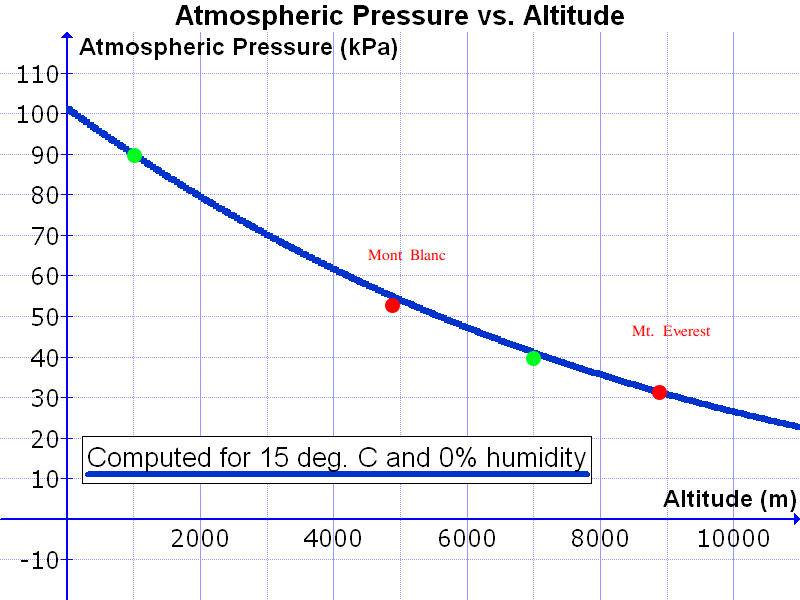
\includegraphics{Atmospheric_Pressure_vs._Altitude.png}
\caption{Atmospheric pressure versus altitude (wikipedia). Green points
represent our measurements, red points represent
interpolation/extrapolation.}
\end{figure}

    \hypertarget{discount-curve-interpolation}{%
\subsection{Discount curve
interpolation}\label{discount-curve-interpolation}}

Now we can come back to finance and using what we have just learnt try
to write a function which interpolates some given discount factors.

Needed data: * a list of pillars dates specifying the value dates of the
given discount factors, \(t_0,...,t_{n-1}\) * a list of given discount
factors, \(D(t_0),...,D(t_{n-1})\) * a pricing date (`today' date) which
corresponds to \(t=0\)

The input argument to the function will be the value date at which we
want to interpolate the discount factor.

Since the discount factor can be expresses as \(D=e^{-r(T-t)}\) the
function will use a log-linear interpolation to return the value we are
looking for.

\[D(t) = \mathrm{exp}\Big( (1-w)\cdot \mathrm{ln}(D(t_i)) + w\cdot \mathrm{ln}(D(t_{i+1}))\Big);\;\;\;w=\frac{t-t_i}{t_{i+1}-t_i}\]

where \(i\) is such that \(t_i \le t \le t_{i+1}\). More technically we
can say that we are doing a linear interpolation over time in the log
space:

\[d(t_i):=\mathrm{ln}(D(t_i))\]

\[d(t) = (1-w)d(t_i) + wd(t_{i+1});\;\;\;w=\frac{t-t_i}{t_{i+1}-t_i}\]

\[D(t) = \mathrm{exp}(d(t))\]

where \(i\) is such that \(t_i \le t \le t_{i+1}\)

Instead of reinventing the wheel and perform the interpolation with our
own code, we'll use the function \texttt{interp} provided by the Python
module \texttt{numpy}. So first let's try it with some simple examples:

    \begin{Verbatim}[commandchars=\\\{\}]
{\color{incolor}In [{\color{incolor}8}]:} \PY{c+c1}{\PYZsh{} let\PYZsq{}s assume we have a list \PYZsq{}xp\PYZsq{} of x-axis coordinates,}
        \PY{c+c1}{\PYZsh{} and the corresponding values \PYZsq{}fp\PYZsq{} of a function evaluated }
        \PY{c+c1}{\PYZsh{} at those x coordinates.}
        \PY{n}{xp} \PY{o}{=} \PY{p}{[}\PY{l+m+mi}{1}\PY{p}{,} \PY{l+m+mi}{2}\PY{p}{,} \PY{l+m+mi}{3}\PY{p}{]}
        \PY{n}{fp} \PY{o}{=} \PY{p}{[}\PY{l+m+mf}{0.3}\PY{p}{,} \PY{l+m+mf}{0.4}\PY{p}{,} \PY{l+m+mf}{0.6}\PY{p}{]}
        
        \PY{c+c1}{\PYZsh{} let\PYZsq{}s see what this looks like when plotted on a graph}
        \PY{c+c1}{\PYZsh{} we briefly introduce here the matplotlib module}
        \PY{c+c1}{\PYZsh{} the keyword as allows to give shorter names to modules}
        \PY{k+kn}{from} \PY{n+nn}{matplotlib} \PY{k}{import} \PY{n}{pyplot} \PY{k}{as} \PY{n}{plt}
        \PY{n}{plt}\PY{o}{.}\PY{n}{plot}\PY{p}{(}\PY{n}{xp}\PY{p}{,} \PY{n}{fp}\PY{p}{,} \PY{n}{marker}\PY{o}{=}\PY{l+s+s1}{\PYZsq{}}\PY{l+s+s1}{o}\PY{l+s+s1}{\PYZsq{}}\PY{p}{)}
        \PY{n}{plt}\PY{o}{.}\PY{n}{grid}\PY{p}{(}\PY{k+kc}{True}\PY{p}{)}
        \PY{n}{plt}\PY{o}{.}\PY{n}{show}\PY{p}{(}\PY{p}{)}
\end{Verbatim}

    \begin{center}
    \adjustimage{max size={0.9\linewidth}{0.9\paperheight}}{lecture_3_files/lecture_3_10_0.png}
    \end{center}
    { \hspace*{\fill} \\}
    
    \begin{Verbatim}[commandchars=\\\{\}]
{\color{incolor}In [{\color{incolor}9}]:} \PY{c+c1}{\PYZsh{} the numpy.interp function linearly interpolates these points to }
        \PY{c+c1}{\PYZsh{} estimate the value of f at other x coordinates. }
        \PY{c+c1}{\PYZsh{} For example, say we want to interpolate the points at x = 2.5::}
        \PY{k+kn}{import} \PY{n+nn}{numpy} \PY{k}{as} \PY{n+nn}{np}
        \PY{n}{np}\PY{o}{.}\PY{n}{interp}\PY{p}{(}\PY{l+m+mf}{2.5}\PY{p}{,} \PY{n}{xp}\PY{p}{,} \PY{n}{fp}\PY{p}{)}
\end{Verbatim}

\begin{Verbatim}[commandchars=\\\{\}]
{\color{outcolor}Out[{\color{outcolor}9}]:} 0.5
\end{Verbatim}
            
    \begin{Verbatim}[commandchars=\\\{\}]
{\color{incolor}In [{\color{incolor}10}]:} \PY{c+c1}{\PYZsh{} let\PYZsq{}s see what this looks like when plotted on a graph}
         
         \PY{k+kn}{from} \PY{n+nn}{matplotlib} \PY{k}{import} \PY{n}{pyplot} \PY{k}{as} \PY{n}{plt}
         \PY{n}{plt}\PY{o}{.}\PY{n}{plot}\PY{p}{(}\PY{n}{xp}\PY{p}{,} \PY{n}{fp}\PY{p}{,} \PY{n}{marker}\PY{o}{=}\PY{l+s+s1}{\PYZsq{}}\PY{l+s+s1}{o}\PY{l+s+s1}{\PYZsq{}}\PY{p}{)}
         \PY{n}{plt}\PY{o}{.}\PY{n}{grid}\PY{p}{(}\PY{k+kc}{True}\PY{p}{)}
         \PY{n}{plt}\PY{o}{.}\PY{n}{plot}\PY{p}{(}\PY{l+m+mf}{2.5}\PY{p}{,} \PY{n}{np}\PY{o}{.}\PY{n}{interp}\PY{p}{(}\PY{l+m+mf}{2.5}\PY{p}{,} \PY{n}{xp}\PY{p}{,} \PY{n}{fp}\PY{p}{)}\PY{p}{,} \PY{n}{marker}\PY{o}{=}\PY{l+s+s1}{\PYZsq{}}\PY{l+s+s1}{X}\PY{l+s+s1}{\PYZsq{}}\PY{p}{)}
         \PY{n}{plt}\PY{o}{.}\PY{n}{show}\PY{p}{(}\PY{p}{)}
\end{Verbatim}

    \begin{center}
    \adjustimage{max size={0.9\linewidth}{0.9\paperheight}}{lecture_3_files/lecture_3_12_0.png}
    \end{center}
    { \hspace*{\fill} \\}
    
    \hypertarget{interlude}{%
\subsubsection{Interlude}\label{interlude}}

How to learn about a given function ? Use the \texttt{help} keyword !

    \begin{Verbatim}[commandchars=\\\{\}]
{\color{incolor}In [{\color{incolor}11}]:} \PY{n}{help}\PY{p}{(}\PY{n}{np}\PY{o}{.}\PY{n}{interp}\PY{p}{)}
\end{Verbatim}

    \begin{Verbatim}[commandchars=\\\{\}]
Help on function interp in module numpy:

interp(x, xp, fp, left=None, right=None, period=None)
    One-dimensional linear interpolation.
    
    Returns the one-dimensional piecewise linear interpolant to a function
    with given discrete data points (`xp`, `fp`), evaluated at `x`.
    
    Parameters
    ----------
    x : array\_like
        The x-coordinates at which to evaluate the interpolated values.
    
    xp : 1-D sequence of floats
        The x-coordinates of the data points, must be increasing if argument
        `period` is not specified. Otherwise, `xp` is internally sorted after
        normalizing the periodic boundaries with ``xp = xp \% period``.
    
    fp : 1-D sequence of float or complex
        The y-coordinates of the data points, same length as `xp`.
    
    left : optional float or complex corresponding to fp
        Value to return for `x < xp[0]`, default is `fp[0]`.
    
    right : optional float or complex corresponding to fp
        Value to return for `x > xp[-1]`, default is `fp[-1]`.
    
    period : None or float, optional
        A period for the x-coordinates. This parameter allows the proper
        interpolation of angular x-coordinates. Parameters `left` and `right`
        are ignored if `period` is specified.
    
        .. versionadded:: 1.10.0
    
    Returns
    -------
    y : float or complex (corresponding to fp) or ndarray
        The interpolated values, same shape as `x`.
    
    Raises
    ------
    ValueError
        If `xp` and `fp` have different length
        If `xp` or `fp` are not 1-D sequences
        If `period == 0`
    
    Notes
    -----
    Does not check that the x-coordinate sequence `xp` is increasing.
    If `xp` is not increasing, the results are nonsense.
    A simple check for increasing is::
    
        np.all(np.diff(xp) > 0)
    
    Examples
    --------
    >>> xp = [1, 2, 3]
    >>> fp = [3, 2, 0]
    >>> np.interp(2.5, xp, fp)
    1.0
    >>> np.interp([0, 1, 1.5, 2.72, 3.14], xp, fp)
    array([ 3. ,  3. ,  2.5 ,  0.56,  0. ])
    >>> UNDEF = -99.0
    >>> np.interp(3.14, xp, fp, right=UNDEF)
    -99.0
    
    Plot an interpolant to the sine function:
    
    >>> x = np.linspace(0, 2*np.pi, 10)
    >>> y = np.sin(x)
    >>> xvals = np.linspace(0, 2*np.pi, 50)
    >>> yinterp = np.interp(xvals, x, y)
    >>> import matplotlib.pyplot as plt
    >>> plt.plot(x, y, 'o')
    [<matplotlib.lines.Line2D object at 0x{\ldots}>]
    >>> plt.plot(xvals, yinterp, '-x')
    [<matplotlib.lines.Line2D object at 0x{\ldots}>]
    >>> plt.show()
    
    Interpolation with periodic x-coordinates:
    
    >>> x = [-180, -170, -185, 185, -10, -5, 0, 365]
    >>> xp = [190, -190, 350, -350]
    >>> fp = [5, 10, 3, 4]
    >>> np.interp(x, xp, fp, period=360)
    array([7.5, 5., 8.75, 6.25, 3., 3.25, 3.5, 3.75])
    
    Complex interpolation:
    
    >>> x = [1.5, 4.0]
    >>> xp = [2,3,5]
    >>> fp = [1.0j, 0, 2+3j]
    >>> np.interp(x, xp, fp)
    array([ 0.+1.j ,  1.+1.5j])


    \end{Verbatim}

    \hypertarget{now-back-to-our-discount-factor-function-df.}{%
\subsubsection{Now back to our discount factor function
df.}\label{now-back-to-our-discount-factor-function-df.}}

    \begin{Verbatim}[commandchars=\\\{\}]
{\color{incolor}In [{\color{incolor}12}]:} \PY{c+c1}{\PYZsh{} import modules and objects that we need}
         \PY{k+kn}{from} \PY{n+nn}{datetime} \PY{k}{import} \PY{n}{date}
         \PY{k+kn}{import} \PY{n+nn}{numpy}\PY{o}{,} \PY{n+nn}{math}
         \PY{k+kn}{from} \PY{n+nn}{matplotlib} \PY{k}{import} \PY{n}{pyplot} \PY{k}{as} \PY{n}{plt}
         \PY{k+kn}{import} \PY{n+nn}{matplotlib}\PY{n+nn}{.}\PY{n+nn}{dates} \PY{k}{as} \PY{n+nn}{mdates} 
         \PY{c+c1}{\PYZsh{} with this notation we tell python to use mdates as an alias }
         \PY{c+c1}{\PYZsh{} for matplotlib.dates, I told you I\PYZsq{}m lazy...}
         
         \PY{c+c1}{\PYZsh{} define the input data}
         \PY{n}{today\PYZus{}date} \PY{o}{=} \PY{n}{date}\PY{p}{(}\PY{l+m+mi}{2019}\PY{p}{,} \PY{l+m+mi}{10}\PY{p}{,} \PY{l+m+mi}{1}\PY{p}{)}
         
         \PY{n}{pillar\PYZus{}dates} \PY{o}{=} \PY{p}{[}\PY{n}{date}\PY{p}{(}\PY{l+m+mi}{2019}\PY{p}{,} \PY{l+m+mi}{10}\PY{p}{,} \PY{l+m+mi}{1}\PY{p}{)}\PY{p}{,} \PY{n}{date}\PY{p}{(}\PY{l+m+mi}{2020}\PY{p}{,} \PY{l+m+mi}{10}\PY{p}{,} \PY{l+m+mi}{1}\PY{p}{)}\PY{p}{,} \PY{n}{date}\PY{p}{(}\PY{l+m+mi}{2021}\PY{p}{,} \PY{l+m+mi}{10}\PY{p}{,} \PY{l+m+mi}{1}\PY{p}{)}\PY{p}{]}
         \PY{n}{discount\PYZus{}factors} \PY{o}{=} \PY{p}{[}\PY{l+m+mf}{1.0}\PY{p}{,} \PY{l+m+mf}{0.97}\PY{p}{,} \PY{l+m+mf}{0.72}\PY{p}{]}
         
         \PY{c+c1}{\PYZsh{} let\PYZsq{}s see what this looks like when plotted on a graph}
         \PY{c+c1}{\PYZsh{} here a more complicated usage of matplotlib to}
         \PY{c+c1}{\PYZsh{} get a nicer plot}
         \PY{n}{plt}\PY{o}{.}\PY{n}{plot}\PY{p}{(}\PY{n}{pillar\PYZus{}dates}\PY{p}{,} \PY{n}{discount\PYZus{}factors}\PY{p}{,} \PY{n}{marker}\PY{o}{=}\PY{l+s+s1}{\PYZsq{}}\PY{l+s+s1}{o}\PY{l+s+s1}{\PYZsq{}}\PY{p}{)}
         \PY{n}{plt}\PY{o}{.}\PY{n}{gca}\PY{p}{(}\PY{p}{)}\PY{o}{.}\PY{n}{xaxis}\PY{o}{.}\PY{n}{set\PYZus{}major\PYZus{}formatter}\PY{p}{(}\PY{n}{mdates}\PY{o}{.}\PY{n}{DateFormatter}\PY{p}{(}\PY{l+s+s1}{\PYZsq{}}\PY{l+s+s1}{\PYZpc{}}\PY{l+s+s1}{m/}\PY{l+s+si}{\PYZpc{}d}\PY{l+s+s1}{/}\PY{l+s+s1}{\PYZpc{}}\PY{l+s+s1}{Y}\PY{l+s+s1}{\PYZsq{}}\PY{p}{)}\PY{p}{)}
         \PY{n}{plt}\PY{o}{.}\PY{n}{gca}\PY{p}{(}\PY{p}{)}\PY{o}{.}\PY{n}{xaxis}\PY{o}{.}\PY{n}{set\PYZus{}major\PYZus{}locator}\PY{p}{(}\PY{n}{mdates}\PY{o}{.}\PY{n}{YearLocator}\PY{p}{(}\PY{p}{)}\PY{p}{)}
         \PY{n}{plt}\PY{o}{.}\PY{n}{grid}\PY{p}{(}\PY{k+kc}{True}\PY{p}{)}
         \PY{n}{plt}\PY{o}{.}\PY{n}{show}\PY{p}{(}\PY{p}{)}
         
         \PY{c+c1}{\PYZsh{} define the df function}
         \PY{k}{def} \PY{n+nf}{df}\PY{p}{(}\PY{n}{d}\PY{p}{)}\PY{p}{:}
             \PY{c+c1}{\PYZsh{} first thing we need to do is to apply the logarithm function }
             \PY{c+c1}{\PYZsh{} to the discount factors since we are doing log-linear and}
             \PY{c+c1}{\PYZsh{} not just linear interpolation}
             \PY{n}{log\PYZus{}discount\PYZus{}factors} \PY{o}{=} \PY{p}{[}\PY{p}{]}
             \PY{k}{for} \PY{n}{discount\PYZus{}factor} \PY{o+ow}{in} \PY{n}{discount\PYZus{}factors}\PY{p}{:}
                 \PY{n}{log\PYZus{}discount\PYZus{}factors}\PY{o}{.}\PY{n}{append}\PY{p}{(}\PY{n}{math}\PY{o}{.}\PY{n}{log}\PY{p}{(}\PY{n}{discount\PYZus{}factor}\PY{p}{)}\PY{p}{)}
             
             \PY{c+c1}{\PYZsh{} perform the linear interpolation of the log discount factors}
             \PY{n}{interpolated\PYZus{}log\PYZus{}discount\PYZus{}factor} \PY{o}{=} \PYZbs{}
                 \PY{n}{numpy}\PY{o}{.}\PY{n}{interp}\PY{p}{(}\PY{n}{d}\PY{p}{,} \PY{n}{pillar\PYZus{}dates}\PY{p}{,} \PY{n}{log\PYZus{}discount\PYZus{}factors}\PY{p}{)}
             
             \PY{c+c1}{\PYZsh{} return the interpolated discount factor}
             \PY{k}{return} \PY{n}{math}\PY{o}{.}\PY{n}{exp}\PY{p}{(}\PY{n}{interpolated\PYZus{}log\PYZus{}discount\PYZus{}factor}\PY{p}{)}
\end{Verbatim}

    \begin{center}
    \adjustimage{max size={0.9\linewidth}{0.9\paperheight}}{lecture_3_files/lecture_3_16_0.png}
    \end{center}
    { \hspace*{\fill} \\}
    
    This is almost OK, \textbf{but it won't work} because
\texttt{numpy.interp} only accepts numbers/lists of numbers as arguments
i.e.~it doesn't automatically convert or interpret dates as numbers in
any way, so it doesn't know how to interpolate them. So we need to do
the conversion ourselves before passing the data into the
\texttt{numpy.interp} function.

    \begin{Verbatim}[commandchars=\\\{\}]
{\color{incolor}In [{\color{incolor}13}]:} \PY{k}{def} \PY{n+nf}{df}\PY{p}{(}\PY{n}{d}\PY{p}{)}\PY{p}{:}
             \PY{c+c1}{\PYZsh{} first thing we need to do is to apply the logarithm function}
             \PY{c+c1}{\PYZsh{} to the discount factors since we are doing log-linear and}
             \PY{c+c1}{\PYZsh{} not just linear interpolation}
             \PY{n}{log\PYZus{}discount\PYZus{}factors} \PY{o}{=} \PY{p}{[}\PY{p}{]}
             \PY{k}{for} \PY{n}{discount\PYZus{}factor} \PY{o+ow}{in} \PY{n}{discount\PYZus{}factors}\PY{p}{:}
                 \PY{n}{log\PYZus{}discount\PYZus{}factors}\PY{o}{.}\PY{n}{append}\PY{p}{(}\PY{n}{math}\PY{o}{.}\PY{n}{log}\PY{p}{(}\PY{n}{discount\PYZus{}factor}\PY{p}{)}\PY{p}{)}
             
             \PY{c+c1}{\PYZsh{} convert the pillar dates to pillar \PYZsq{}days\PYZsq{}}
             \PY{c+c1}{\PYZsh{} i.e. number of days from today}
             \PY{c+c1}{\PYZsh{} to write shorter code we can use this NEW notation}
             \PY{c+c1}{\PYZsh{} which condenses for and list creation in one line}
             \PY{n}{pillar\PYZus{}days} \PY{o}{=} \PYZbs{}
                 \PY{p}{[}\PY{p}{(}\PY{n}{pillar\PYZus{}date} \PY{o}{\PYZhy{}} \PY{n}{today\PYZus{}date}\PY{p}{)}\PY{o}{.}\PY{n}{days} \PY{k}{for} \PY{n}{pillar\PYZus{}date} \PY{o+ow}{in} \PY{n}{pillar\PYZus{}dates}\PY{p}{]}
             
             \PY{c+c1}{\PYZsh{} obviously we need to do the same to the value date}
             \PY{c+c1}{\PYZsh{} argument of the df function}
             \PY{n}{d\PYZus{}days} \PY{o}{=} \PY{p}{(}\PY{n}{d} \PY{o}{\PYZhy{}} \PY{n}{today\PYZus{}date}\PY{p}{)}\PY{o}{.}\PY{n}{days}
             
             \PY{c+c1}{\PYZsh{} perform the linear interpolation of the log discount factors}
             \PY{n}{interpolated\PYZus{}log\PYZus{}discount\PYZus{}factor} \PY{o}{=} \PYZbs{}
                 \PY{n}{numpy}\PY{o}{.}\PY{n}{interp}\PY{p}{(}\PY{n}{d\PYZus{}days}\PY{p}{,} \PY{n}{pillar\PYZus{}days}\PY{p}{,} \PY{n}{log\PYZus{}discount\PYZus{}factors}\PY{p}{)}
             
             \PY{c+c1}{\PYZsh{} return the interpolated discount factor}
             \PY{k}{return} \PY{n}{math}\PY{o}{.}\PY{n}{exp}\PY{p}{(}\PY{n}{interpolated\PYZus{}log\PYZus{}discount\PYZus{}factor}\PY{p}{)}
\end{Verbatim}

    \begin{Verbatim}[commandchars=\\\{\}]
{\color{incolor}In [{\color{incolor}18}]:} \PY{c+c1}{\PYZsh{} now we can use the df function to get discount factors}
         \PY{c+c1}{\PYZsh{} on value dates between the given pillar dates}
         \PY{n}{d0} \PY{o}{=} \PY{n}{date}\PY{p}{(}\PY{l+m+mi}{2020}\PY{p}{,} \PY{l+m+mi}{1}\PY{p}{,} \PY{l+m+mi}{1}\PY{p}{)}
         \PY{n}{df0} \PY{o}{=} \PY{n}{df}\PY{p}{(}\PY{n}{d0}\PY{p}{)}
         \PY{n+nb}{print} \PY{p}{(}\PY{n}{df0}\PY{p}{)}
\end{Verbatim}

    \begin{Verbatim}[commandchars=\\\{\}]
0.9923728228571693

    \end{Verbatim}

    \begin{Verbatim}[commandchars=\\\{\}]
{\color{incolor}In [{\color{incolor}15}]:} \PY{n}{d1} \PY{o}{=} \PY{n}{date}\PY{p}{(}\PY{l+m+mi}{2021}\PY{p}{,} \PY{l+m+mi}{1}\PY{p}{,} \PY{l+m+mi}{1}\PY{p}{)}
         \PY{n}{df1} \PY{o}{=} \PY{n}{df}\PY{p}{(}\PY{n}{d1}\PY{p}{)}
         \PY{n+nb}{print} \PY{p}{(}\PY{n}{df1}\PY{p}{)}
\end{Verbatim}

    \begin{Verbatim}[commandchars=\\\{\}]
0.8997999273630835

    \end{Verbatim}

    \begin{Verbatim}[commandchars=\\\{\}]
{\color{incolor}In [{\color{incolor}19}]:} \PY{c+c1}{\PYZsh{} let\PYZsq{}s see what these look like when plotted on a semi-log graph}
         
         \PY{k+kn}{from} \PY{n+nn}{matplotlib} \PY{k}{import} \PY{n}{pyplot} \PY{k}{as} \PY{n}{plt}
         \PY{k+kn}{import} \PY{n+nn}{matplotlib}\PY{n+nn}{.}\PY{n+nn}{dates} \PY{k}{as} \PY{n+nn}{mdates}
         \PY{n}{plt}\PY{o}{.}\PY{n}{semilogy}\PY{p}{(}\PY{n}{pillar\PYZus{}dates}\PY{p}{,} \PY{n}{discount\PYZus{}factors}\PY{p}{,} \PY{n}{marker}\PY{o}{=}\PY{l+s+s1}{\PYZsq{}}\PY{l+s+s1}{o}\PY{l+s+s1}{\PYZsq{}}\PY{p}{)}
         \PY{n}{plt}\PY{o}{.}\PY{n}{semilogy}\PY{p}{(}\PY{n}{d0}\PY{p}{,}\PY{n}{df0} \PY{p}{,} \PY{n}{marker}\PY{o}{=}\PY{l+s+s1}{\PYZsq{}}\PY{l+s+s1}{X}\PY{l+s+s1}{\PYZsq{}}\PY{p}{)}
         \PY{n}{plt}\PY{o}{.}\PY{n}{semilogy}\PY{p}{(}\PY{n}{d1}\PY{p}{,}\PY{n}{df1} \PY{p}{,} \PY{n}{marker}\PY{o}{=}\PY{l+s+s1}{\PYZsq{}}\PY{l+s+s1}{X}\PY{l+s+s1}{\PYZsq{}}\PY{p}{)}
         \PY{n}{plt}\PY{o}{.}\PY{n}{gca}\PY{p}{(}\PY{p}{)}\PY{o}{.}\PY{n}{xaxis}\PY{o}{.}\PY{n}{set\PYZus{}major\PYZus{}formatter}\PY{p}{(}\PY{n}{mdates}\PY{o}{.}\PY{n}{DateFormatter}\PY{p}{(}\PY{l+s+s1}{\PYZsq{}}\PY{l+s+s1}{\PYZpc{}}\PY{l+s+s1}{m/}\PY{l+s+si}{\PYZpc{}d}\PY{l+s+s1}{/}\PY{l+s+s1}{\PYZpc{}}\PY{l+s+s1}{Y}\PY{l+s+s1}{\PYZsq{}}\PY{p}{)}\PY{p}{)}
         \PY{n}{plt}\PY{o}{.}\PY{n}{gca}\PY{p}{(}\PY{p}{)}\PY{o}{.}\PY{n}{xaxis}\PY{o}{.}\PY{n}{set\PYZus{}major\PYZus{}locator}\PY{p}{(}\PY{n}{mdates}\PY{o}{.}\PY{n}{YearLocator}\PY{p}{(}\PY{p}{)}\PY{p}{)}
         \PY{n}{plt}\PY{o}{.}\PY{n}{grid}\PY{p}{(}\PY{k+kc}{True}\PY{p}{)}
         \PY{n}{plt}\PY{o}{.}\PY{n}{show}\PY{p}{(}\PY{p}{)}
\end{Verbatim}

    \begin{center}
    \adjustimage{max size={0.9\linewidth}{0.9\paperheight}}{lecture_3_files/lecture_3_21_0.png}
    \end{center}
    { \hspace*{\fill} \\}
    
    \begin{Verbatim}[commandchars=\\\{\}]
{\color{incolor}In [{\color{incolor}20}]:} \PY{c+c1}{\PYZsh{} let\PYZsq{}s see what these look like when plotted on a linear graph}
         
         \PY{k+kn}{from} \PY{n+nn}{matplotlib} \PY{k}{import} \PY{n}{pyplot} \PY{k}{as} \PY{n}{plt}
         \PY{k+kn}{import} \PY{n+nn}{matplotlib}\PY{n+nn}{.}\PY{n+nn}{dates} \PY{k}{as} \PY{n+nn}{mdates}
         \PY{n}{plt}\PY{o}{.}\PY{n}{plot}\PY{p}{(}\PY{n}{pillar\PYZus{}dates}\PY{p}{,} \PY{n}{discount\PYZus{}factors}\PY{p}{,} \PY{n}{marker}\PY{o}{=}\PY{l+s+s1}{\PYZsq{}}\PY{l+s+s1}{o}\PY{l+s+s1}{\PYZsq{}}\PY{p}{)}
         \PY{n}{plt}\PY{o}{.}\PY{n}{plot}\PY{p}{(}\PY{n}{d0}\PY{p}{,}\PY{n}{df0} \PY{p}{,} \PY{n}{marker}\PY{o}{=}\PY{l+s+s1}{\PYZsq{}}\PY{l+s+s1}{X}\PY{l+s+s1}{\PYZsq{}}\PY{p}{)}
         \PY{n}{plt}\PY{o}{.}\PY{n}{plot}\PY{p}{(}\PY{n}{d1}\PY{p}{,}\PY{n}{df1} \PY{p}{,} \PY{n}{marker}\PY{o}{=}\PY{l+s+s1}{\PYZsq{}}\PY{l+s+s1}{X}\PY{l+s+s1}{\PYZsq{}}\PY{p}{)}
         \PY{n}{plt}\PY{o}{.}\PY{n}{gca}\PY{p}{(}\PY{p}{)}\PY{o}{.}\PY{n}{xaxis}\PY{o}{.}\PY{n}{set\PYZus{}major\PYZus{}formatter}\PY{p}{(}\PY{n}{mdates}\PY{o}{.}\PY{n}{DateFormatter}\PY{p}{(}\PY{l+s+s1}{\PYZsq{}}\PY{l+s+s1}{\PYZpc{}}\PY{l+s+s1}{m/}\PY{l+s+si}{\PYZpc{}d}\PY{l+s+s1}{/}\PY{l+s+s1}{\PYZpc{}}\PY{l+s+s1}{Y}\PY{l+s+s1}{\PYZsq{}}\PY{p}{)}\PY{p}{)}
         \PY{n}{plt}\PY{o}{.}\PY{n}{gca}\PY{p}{(}\PY{p}{)}\PY{o}{.}\PY{n}{xaxis}\PY{o}{.}\PY{n}{set\PYZus{}major\PYZus{}locator}\PY{p}{(}\PY{n}{mdates}\PY{o}{.}\PY{n}{YearLocator}\PY{p}{(}\PY{p}{)}\PY{p}{)}
         \PY{n}{plt}\PY{o}{.}\PY{n}{grid}\PY{p}{(}\PY{k+kc}{True}\PY{p}{)}
         \PY{n}{plt}\PY{o}{.}\PY{n}{show}\PY{p}{(}\PY{p}{)}
\end{Verbatim}

    \begin{center}
    \adjustimage{max size={0.9\linewidth}{0.9\paperheight}}{lecture_3_files/lecture_3_22_0.png}
    \end{center}
    { \hspace*{\fill} \\}
    
    \hypertarget{exercises}{%
\subsection{Exercises}\label{exercises}}

\hypertarget{exercise-3.1}{%
\subsubsection{Exercise 3.1}\label{exercise-3.1}}

Take the code for the Black-Scholes formula from Exercise 2.3 and wrap
it in a function. Then, use this function to calculate the prices of
calls with various strikes, using the following data.

\begin{Shaded}
\begin{Highlighting}[]
\NormalTok{S_t }\OperatorTok{=} \DecValTok{800}
\CommentTok{# strikes expressed as % of spot price}
\NormalTok{moneyness }\OperatorTok{=}\NormalTok{ [ }\FloatTok{0.5}\NormalTok{, }\FloatTok{0.75}\NormalTok{, }\FloatTok{0.825}\NormalTok{, }\FloatTok{1.0}\NormalTok{, }\FloatTok{1.125}\NormalTok{, }\FloatTok{1.25}\NormalTok{, }\FloatTok{1.5}\NormalTok{ ]   }
\NormalTok{vol }\OperatorTok{=} \FloatTok{0.3}
\NormalTok{ttm }\OperatorTok{=} \FloatTok{0.75}
\NormalTok{r }\OperatorTok{=} \FloatTok{0.005}
\end{Highlighting}
\end{Shaded}

The output should be a dictionary mapping strikes to call prices.

\hypertarget{exercise-3.2}{%
\subsubsection{Exercise 3.2}\label{exercise-3.2}}

Python has a useful command called \texttt{assert} which can be used for
checking that a given condition is satisfied, and raising an error if
the condition is not satisfied.

The following line does not cause an error, in fact it does nothing

\begin{Shaded}
\begin{Highlighting}[]
\ControlFlowTok{assert} \DecValTok{1} \OperatorTok{<} \DecValTok{2}
\end{Highlighting}
\end{Shaded}

This causes an error

\begin{Shaded}
\begin{Highlighting}[]
\ControlFlowTok{assert} \DecValTok{1} \OperatorTok{>} \DecValTok{2}
\end{Highlighting}
\end{Shaded}

\texttt{assert} can take a second parameter with a message to display in case of failure:

\begin{Shaded}
\begin{Highlighting}[]
\ControlFlowTok{assert} \DecValTok{1} \OperatorTok{>} \DecValTok{2}, ``Two is bigger than one''
\end{Highlighting}
\end{Shaded}

Take the \texttt{df} function from this lesson and modify it by adding some
assertions to check that:
\begin{itemize}
\item the pillar date list contains at least 2 elements
\item the pillar date list is the same length as the discount factor list
\item the first pillar date is equal to the today date
\item the value date argument 'd' is greater or equal to the first pillar date and also less than or equal to the last pillar date
\end{itemize}

Then try using the function with some invalid data to make sure that
your assertions are correctly checking the desired conditions.

\hypertarget{exercise-3.3}{%
\subsubsection{Exercise 3.3}\label{exercise-3.3}}

Python has a module called \texttt{matplotlib} which can be used for
plotting graphs and charts. In particular, we can use a sub-module
called \texttt{pyplot} which provides slightly easier-to-use interface
for plotting interactively.

\begin{Shaded}
\begin{Highlighting}[]
\ImportTok{from}\NormalTok{ matplotlib }\ImportTok{import}\NormalTok{ pyplot}

\CommentTok{# plot some data}
\NormalTok{pyplot.plot(}
\NormalTok{    [}\DecValTok{1}\NormalTok{, }\DecValTok{2}\NormalTok{, }\DecValTok{3}\NormalTok{],   }\CommentTok{# x-axis coordinates}
\NormalTok{    [}\DecValTok{5}\NormalTok{, }\DecValTok{3}\NormalTok{, }\DecValTok{10}\NormalTok{],  }\CommentTok{# y-axis coordinates}
\NormalTok{    marker}\OperatorTok{=}\StringTok{'o'}   \CommentTok{# we want the points to be marked with circles}
\NormalTok{)}
\end{Highlighting}
\end{Shaded}

Use this function to plot the call prices from exercise 3.1. Remember to
use \texttt{help} and \texttt{dir} to have some help (or to look in
Google ;-)).

    \hypertarget{advanced-hint}{%
\subsection{Advanced hint}\label{advanced-hint}}

Interpolation using \texttt{scipy.interpolate}:
https://docs.scipy.org/doc/scipy-0.15.1/reference/interpolate.html\#module-scipy.interpolate


    % Add a bibliography block to the postdoc
    
    
    
    \end{document}

%\clearpage
%
% Default to the notebook output style

    


% Inherit from the specified cell style.




    
\documentclass[11pt]{article}

    
    
    \usepackage[T1]{fontenc}
    % Nicer default font (+ math font) than Computer Modern for most use cases
    \usepackage{mathpazo}

    % Basic figure setup, for now with no caption control since it's done
    % automatically by Pandoc (which extracts ![](path) syntax from Markdown).
    \usepackage{graphicx}
    % We will generate all images so they have a width \maxwidth. This means
    % that they will get their normal width if they fit onto the page, but
    % are scaled down if they would overflow the margins.
    \makeatletter
    \def\maxwidth{\ifdim\Gin@nat@width>\linewidth\linewidth
    \else\Gin@nat@width\fi}
    \makeatother
    \let\Oldincludegraphics\includegraphics
    % Set max figure width to be 80% of text width, for now hardcoded.
    \renewcommand{\includegraphics}[1]{\Oldincludegraphics[width=.8\maxwidth]{#1}}
    % Ensure that by default, figures have no caption (until we provide a
    % proper Figure object with a Caption API and a way to capture that
    % in the conversion process - todo).
    \usepackage{caption}
    \DeclareCaptionLabelFormat{nolabel}{}
    \captionsetup{labelformat=nolabel}

    \usepackage{adjustbox} % Used to constrain images to a maximum size 
    \usepackage{xcolor} % Allow colors to be defined
    \usepackage{enumerate} % Needed for markdown enumerations to work
    \usepackage{geometry} % Used to adjust the document margins
    \usepackage{amsmath} % Equations
    \usepackage{amssymb} % Equations
    \usepackage{textcomp} % defines textquotesingle
    % Hack from http://tex.stackexchange.com/a/47451/13684:
    \AtBeginDocument{%
        \def\PYZsq{\textquotesingle}% Upright quotes in Pygmentized code
    }
    \usepackage{upquote} % Upright quotes for verbatim code
    \usepackage{eurosym} % defines \euro
    \usepackage[mathletters]{ucs} % Extended unicode (utf-8) support
    \usepackage[utf8x]{inputenc} % Allow utf-8 characters in the tex document
    \usepackage{fancyvrb} % verbatim replacement that allows latex
    \usepackage{grffile} % extends the file name processing of package graphics 
                         % to support a larger range 
    % The hyperref package gives us a pdf with properly built
    % internal navigation ('pdf bookmarks' for the table of contents,
    % internal cross-reference links, web links for URLs, etc.)
    \usepackage{hyperref}
    \usepackage{longtable} % longtable support required by pandoc >1.10
    \usepackage{booktabs}  % table support for pandoc > 1.12.2
    \usepackage[inline]{enumitem} % IRkernel/repr support (it uses the enumerate* environment)
    \usepackage[normalem]{ulem} % ulem is needed to support strikethroughs (\sout)
                                % normalem makes italics be italics, not underlines
    \usepackage{mathrsfs}
    

    
    
    % Colors for the hyperref package
    \definecolor{urlcolor}{rgb}{0,.145,.698}
    \definecolor{linkcolor}{rgb}{.71,0.21,0.01}
    \definecolor{citecolor}{rgb}{.12,.54,.11}

    % ANSI colors
    \definecolor{ansi-black}{HTML}{3E424D}
    \definecolor{ansi-black-intense}{HTML}{282C36}
    \definecolor{ansi-red}{HTML}{E75C58}
    \definecolor{ansi-red-intense}{HTML}{B22B31}
    \definecolor{ansi-green}{HTML}{00A250}
    \definecolor{ansi-green-intense}{HTML}{007427}
    \definecolor{ansi-yellow}{HTML}{DDB62B}
    \definecolor{ansi-yellow-intense}{HTML}{B27D12}
    \definecolor{ansi-blue}{HTML}{208FFB}
    \definecolor{ansi-blue-intense}{HTML}{0065CA}
    \definecolor{ansi-magenta}{HTML}{D160C4}
    \definecolor{ansi-magenta-intense}{HTML}{A03196}
    \definecolor{ansi-cyan}{HTML}{60C6C8}
    \definecolor{ansi-cyan-intense}{HTML}{258F8F}
    \definecolor{ansi-white}{HTML}{C5C1B4}
    \definecolor{ansi-white-intense}{HTML}{A1A6B2}
    \definecolor{ansi-default-inverse-fg}{HTML}{FFFFFF}
    \definecolor{ansi-default-inverse-bg}{HTML}{000000}

    % commands and environments needed by pandoc snippets
    % extracted from the output of `pandoc -s`
    \providecommand{\tightlist}{%
      \setlength{\itemsep}{0pt}\setlength{\parskip}{0pt}}
    \DefineVerbatimEnvironment{Highlighting}{Verbatim}{commandchars=\\\{\}}
    % Add ',fontsize=\small' for more characters per line
    \newenvironment{Shaded}{}{}
    \newcommand{\KeywordTok}[1]{\textcolor[rgb]{0.00,0.44,0.13}{\textbf{{#1}}}}
    \newcommand{\DataTypeTok}[1]{\textcolor[rgb]{0.56,0.13,0.00}{{#1}}}
    \newcommand{\DecValTok}[1]{\textcolor[rgb]{0.25,0.63,0.44}{{#1}}}
    \newcommand{\BaseNTok}[1]{\textcolor[rgb]{0.25,0.63,0.44}{{#1}}}
    \newcommand{\FloatTok}[1]{\textcolor[rgb]{0.25,0.63,0.44}{{#1}}}
    \newcommand{\CharTok}[1]{\textcolor[rgb]{0.25,0.44,0.63}{{#1}}}
    \newcommand{\StringTok}[1]{\textcolor[rgb]{0.25,0.44,0.63}{{#1}}}
    \newcommand{\CommentTok}[1]{\textcolor[rgb]{0.38,0.63,0.69}{\textit{{#1}}}}
    \newcommand{\OtherTok}[1]{\textcolor[rgb]{0.00,0.44,0.13}{{#1}}}
    \newcommand{\AlertTok}[1]{\textcolor[rgb]{1.00,0.00,0.00}{\textbf{{#1}}}}
    \newcommand{\FunctionTok}[1]{\textcolor[rgb]{0.02,0.16,0.49}{{#1}}}
    \newcommand{\RegionMarkerTok}[1]{{#1}}
    \newcommand{\ErrorTok}[1]{\textcolor[rgb]{1.00,0.00,0.00}{\textbf{{#1}}}}
    \newcommand{\NormalTok}[1]{{#1}}
    
    % Additional commands for more recent versions of Pandoc
    \newcommand{\ConstantTok}[1]{\textcolor[rgb]{0.53,0.00,0.00}{{#1}}}
    \newcommand{\SpecialCharTok}[1]{\textcolor[rgb]{0.25,0.44,0.63}{{#1}}}
    \newcommand{\VerbatimStringTok}[1]{\textcolor[rgb]{0.25,0.44,0.63}{{#1}}}
    \newcommand{\SpecialStringTok}[1]{\textcolor[rgb]{0.73,0.40,0.53}{{#1}}}
    \newcommand{\ImportTok}[1]{{#1}}
    \newcommand{\DocumentationTok}[1]{\textcolor[rgb]{0.73,0.13,0.13}{\textit{{#1}}}}
    \newcommand{\AnnotationTok}[1]{\textcolor[rgb]{0.38,0.63,0.69}{\textbf{\textit{{#1}}}}}
    \newcommand{\CommentVarTok}[1]{\textcolor[rgb]{0.38,0.63,0.69}{\textbf{\textit{{#1}}}}}
    \newcommand{\VariableTok}[1]{\textcolor[rgb]{0.10,0.09,0.49}{{#1}}}
    \newcommand{\ControlFlowTok}[1]{\textcolor[rgb]{0.00,0.44,0.13}{\textbf{{#1}}}}
    \newcommand{\OperatorTok}[1]{\textcolor[rgb]{0.40,0.40,0.40}{{#1}}}
    \newcommand{\BuiltInTok}[1]{{#1}}
    \newcommand{\ExtensionTok}[1]{{#1}}
    \newcommand{\PreprocessorTok}[1]{\textcolor[rgb]{0.74,0.48,0.00}{{#1}}}
    \newcommand{\AttributeTok}[1]{\textcolor[rgb]{0.49,0.56,0.16}{{#1}}}
    \newcommand{\InformationTok}[1]{\textcolor[rgb]{0.38,0.63,0.69}{\textbf{\textit{{#1}}}}}
    \newcommand{\WarningTok}[1]{\textcolor[rgb]{0.38,0.63,0.69}{\textbf{\textit{{#1}}}}}
    
    
    % Define a nice break command that doesn't care if a line doesn't already
    % exist.
    \def\br{\hspace*{\fill} \\* }
    % Math Jax compatibility definitions
    \def\gt{>}
    \def\lt{<}
    \let\Oldtex\TeX
    \let\Oldlatex\LaTeX
    \renewcommand{\TeX}{\textrm{\Oldtex}}
    \renewcommand{\LaTeX}{\textrm{\Oldlatex}}
    % Document parameters
    % Document title
    \title{Swaps and Modules - Practical Lesson 5}
    \author{Matteo Sani \\ \href{mailto:matteosan1@gmail.com}{matteosan1@gmail.com}}
    
    
    
    

    % Pygments definitions
    
\makeatletter
\def\PY@reset{\let\PY@it=\relax \let\PY@bf=\relax%
    \let\PY@ul=\relax \let\PY@tc=\relax%
    \let\PY@bc=\relax \let\PY@ff=\relax}
\def\PY@tok#1{\csname PY@tok@#1\endcsname}
\def\PY@toks#1+{\ifx\relax#1\empty\else%
    \PY@tok{#1}\expandafter\PY@toks\fi}
\def\PY@do#1{\PY@bc{\PY@tc{\PY@ul{%
    \PY@it{\PY@bf{\PY@ff{#1}}}}}}}
\def\PY#1#2{\PY@reset\PY@toks#1+\relax+\PY@do{#2}}

\expandafter\def\csname PY@tok@w\endcsname{\def\PY@tc##1{\textcolor[rgb]{0.73,0.73,0.73}{##1}}}
\expandafter\def\csname PY@tok@c\endcsname{\let\PY@it=\textit\def\PY@tc##1{\textcolor[rgb]{0.25,0.50,0.50}{##1}}}
\expandafter\def\csname PY@tok@cp\endcsname{\def\PY@tc##1{\textcolor[rgb]{0.74,0.48,0.00}{##1}}}
\expandafter\def\csname PY@tok@k\endcsname{\let\PY@bf=\textbf\def\PY@tc##1{\textcolor[rgb]{0.00,0.50,0.00}{##1}}}
\expandafter\def\csname PY@tok@kp\endcsname{\def\PY@tc##1{\textcolor[rgb]{0.00,0.50,0.00}{##1}}}
\expandafter\def\csname PY@tok@kt\endcsname{\def\PY@tc##1{\textcolor[rgb]{0.69,0.00,0.25}{##1}}}
\expandafter\def\csname PY@tok@o\endcsname{\def\PY@tc##1{\textcolor[rgb]{0.40,0.40,0.40}{##1}}}
\expandafter\def\csname PY@tok@ow\endcsname{\let\PY@bf=\textbf\def\PY@tc##1{\textcolor[rgb]{0.67,0.13,1.00}{##1}}}
\expandafter\def\csname PY@tok@nb\endcsname{\def\PY@tc##1{\textcolor[rgb]{0.00,0.50,0.00}{##1}}}
\expandafter\def\csname PY@tok@nf\endcsname{\def\PY@tc##1{\textcolor[rgb]{0.00,0.00,1.00}{##1}}}
\expandafter\def\csname PY@tok@nc\endcsname{\let\PY@bf=\textbf\def\PY@tc##1{\textcolor[rgb]{0.00,0.00,1.00}{##1}}}
\expandafter\def\csname PY@tok@nn\endcsname{\let\PY@bf=\textbf\def\PY@tc##1{\textcolor[rgb]{0.00,0.00,1.00}{##1}}}
\expandafter\def\csname PY@tok@ne\endcsname{\let\PY@bf=\textbf\def\PY@tc##1{\textcolor[rgb]{0.82,0.25,0.23}{##1}}}
\expandafter\def\csname PY@tok@nv\endcsname{\def\PY@tc##1{\textcolor[rgb]{0.10,0.09,0.49}{##1}}}
\expandafter\def\csname PY@tok@no\endcsname{\def\PY@tc##1{\textcolor[rgb]{0.53,0.00,0.00}{##1}}}
\expandafter\def\csname PY@tok@nl\endcsname{\def\PY@tc##1{\textcolor[rgb]{0.63,0.63,0.00}{##1}}}
\expandafter\def\csname PY@tok@ni\endcsname{\let\PY@bf=\textbf\def\PY@tc##1{\textcolor[rgb]{0.60,0.60,0.60}{##1}}}
\expandafter\def\csname PY@tok@na\endcsname{\def\PY@tc##1{\textcolor[rgb]{0.49,0.56,0.16}{##1}}}
\expandafter\def\csname PY@tok@nt\endcsname{\let\PY@bf=\textbf\def\PY@tc##1{\textcolor[rgb]{0.00,0.50,0.00}{##1}}}
\expandafter\def\csname PY@tok@nd\endcsname{\def\PY@tc##1{\textcolor[rgb]{0.67,0.13,1.00}{##1}}}
\expandafter\def\csname PY@tok@s\endcsname{\def\PY@tc##1{\textcolor[rgb]{0.73,0.13,0.13}{##1}}}
\expandafter\def\csname PY@tok@sd\endcsname{\let\PY@it=\textit\def\PY@tc##1{\textcolor[rgb]{0.73,0.13,0.13}{##1}}}
\expandafter\def\csname PY@tok@si\endcsname{\let\PY@bf=\textbf\def\PY@tc##1{\textcolor[rgb]{0.73,0.40,0.53}{##1}}}
\expandafter\def\csname PY@tok@se\endcsname{\let\PY@bf=\textbf\def\PY@tc##1{\textcolor[rgb]{0.73,0.40,0.13}{##1}}}
\expandafter\def\csname PY@tok@sr\endcsname{\def\PY@tc##1{\textcolor[rgb]{0.73,0.40,0.53}{##1}}}
\expandafter\def\csname PY@tok@ss\endcsname{\def\PY@tc##1{\textcolor[rgb]{0.10,0.09,0.49}{##1}}}
\expandafter\def\csname PY@tok@sx\endcsname{\def\PY@tc##1{\textcolor[rgb]{0.00,0.50,0.00}{##1}}}
\expandafter\def\csname PY@tok@m\endcsname{\def\PY@tc##1{\textcolor[rgb]{0.40,0.40,0.40}{##1}}}
\expandafter\def\csname PY@tok@gh\endcsname{\let\PY@bf=\textbf\def\PY@tc##1{\textcolor[rgb]{0.00,0.00,0.50}{##1}}}
\expandafter\def\csname PY@tok@gu\endcsname{\let\PY@bf=\textbf\def\PY@tc##1{\textcolor[rgb]{0.50,0.00,0.50}{##1}}}
\expandafter\def\csname PY@tok@gd\endcsname{\def\PY@tc##1{\textcolor[rgb]{0.63,0.00,0.00}{##1}}}
\expandafter\def\csname PY@tok@gi\endcsname{\def\PY@tc##1{\textcolor[rgb]{0.00,0.63,0.00}{##1}}}
\expandafter\def\csname PY@tok@gr\endcsname{\def\PY@tc##1{\textcolor[rgb]{1.00,0.00,0.00}{##1}}}
\expandafter\def\csname PY@tok@ge\endcsname{\let\PY@it=\textit}
\expandafter\def\csname PY@tok@gs\endcsname{\let\PY@bf=\textbf}
\expandafter\def\csname PY@tok@gp\endcsname{\let\PY@bf=\textbf\def\PY@tc##1{\textcolor[rgb]{0.00,0.00,0.50}{##1}}}
\expandafter\def\csname PY@tok@go\endcsname{\def\PY@tc##1{\textcolor[rgb]{0.53,0.53,0.53}{##1}}}
\expandafter\def\csname PY@tok@gt\endcsname{\def\PY@tc##1{\textcolor[rgb]{0.00,0.27,0.87}{##1}}}
\expandafter\def\csname PY@tok@err\endcsname{\def\PY@bc##1{\setlength{\fboxsep}{0pt}\fcolorbox[rgb]{1.00,0.00,0.00}{1,1,1}{\strut ##1}}}
\expandafter\def\csname PY@tok@kc\endcsname{\let\PY@bf=\textbf\def\PY@tc##1{\textcolor[rgb]{0.00,0.50,0.00}{##1}}}
\expandafter\def\csname PY@tok@kd\endcsname{\let\PY@bf=\textbf\def\PY@tc##1{\textcolor[rgb]{0.00,0.50,0.00}{##1}}}
\expandafter\def\csname PY@tok@kn\endcsname{\let\PY@bf=\textbf\def\PY@tc##1{\textcolor[rgb]{0.00,0.50,0.00}{##1}}}
\expandafter\def\csname PY@tok@kr\endcsname{\let\PY@bf=\textbf\def\PY@tc##1{\textcolor[rgb]{0.00,0.50,0.00}{##1}}}
\expandafter\def\csname PY@tok@bp\endcsname{\def\PY@tc##1{\textcolor[rgb]{0.00,0.50,0.00}{##1}}}
\expandafter\def\csname PY@tok@fm\endcsname{\def\PY@tc##1{\textcolor[rgb]{0.00,0.00,1.00}{##1}}}
\expandafter\def\csname PY@tok@vc\endcsname{\def\PY@tc##1{\textcolor[rgb]{0.10,0.09,0.49}{##1}}}
\expandafter\def\csname PY@tok@vg\endcsname{\def\PY@tc##1{\textcolor[rgb]{0.10,0.09,0.49}{##1}}}
\expandafter\def\csname PY@tok@vi\endcsname{\def\PY@tc##1{\textcolor[rgb]{0.10,0.09,0.49}{##1}}}
\expandafter\def\csname PY@tok@vm\endcsname{\def\PY@tc##1{\textcolor[rgb]{0.10,0.09,0.49}{##1}}}
\expandafter\def\csname PY@tok@sa\endcsname{\def\PY@tc##1{\textcolor[rgb]{0.73,0.13,0.13}{##1}}}
\expandafter\def\csname PY@tok@sb\endcsname{\def\PY@tc##1{\textcolor[rgb]{0.73,0.13,0.13}{##1}}}
\expandafter\def\csname PY@tok@sc\endcsname{\def\PY@tc##1{\textcolor[rgb]{0.73,0.13,0.13}{##1}}}
\expandafter\def\csname PY@tok@dl\endcsname{\def\PY@tc##1{\textcolor[rgb]{0.73,0.13,0.13}{##1}}}
\expandafter\def\csname PY@tok@s2\endcsname{\def\PY@tc##1{\textcolor[rgb]{0.73,0.13,0.13}{##1}}}
\expandafter\def\csname PY@tok@sh\endcsname{\def\PY@tc##1{\textcolor[rgb]{0.73,0.13,0.13}{##1}}}
\expandafter\def\csname PY@tok@s1\endcsname{\def\PY@tc##1{\textcolor[rgb]{0.73,0.13,0.13}{##1}}}
\expandafter\def\csname PY@tok@mb\endcsname{\def\PY@tc##1{\textcolor[rgb]{0.40,0.40,0.40}{##1}}}
\expandafter\def\csname PY@tok@mf\endcsname{\def\PY@tc##1{\textcolor[rgb]{0.40,0.40,0.40}{##1}}}
\expandafter\def\csname PY@tok@mh\endcsname{\def\PY@tc##1{\textcolor[rgb]{0.40,0.40,0.40}{##1}}}
\expandafter\def\csname PY@tok@mi\endcsname{\def\PY@tc##1{\textcolor[rgb]{0.40,0.40,0.40}{##1}}}
\expandafter\def\csname PY@tok@il\endcsname{\def\PY@tc##1{\textcolor[rgb]{0.40,0.40,0.40}{##1}}}
\expandafter\def\csname PY@tok@mo\endcsname{\def\PY@tc##1{\textcolor[rgb]{0.40,0.40,0.40}{##1}}}
\expandafter\def\csname PY@tok@ch\endcsname{\let\PY@it=\textit\def\PY@tc##1{\textcolor[rgb]{0.25,0.50,0.50}{##1}}}
\expandafter\def\csname PY@tok@cm\endcsname{\let\PY@it=\textit\def\PY@tc##1{\textcolor[rgb]{0.25,0.50,0.50}{##1}}}
\expandafter\def\csname PY@tok@cpf\endcsname{\let\PY@it=\textit\def\PY@tc##1{\textcolor[rgb]{0.25,0.50,0.50}{##1}}}
\expandafter\def\csname PY@tok@c1\endcsname{\let\PY@it=\textit\def\PY@tc##1{\textcolor[rgb]{0.25,0.50,0.50}{##1}}}
\expandafter\def\csname PY@tok@cs\endcsname{\let\PY@it=\textit\def\PY@tc##1{\textcolor[rgb]{0.25,0.50,0.50}{##1}}}

\def\PYZbs{\char`\\}
\def\PYZus{\char`\_}
\def\PYZob{\char`\{}
\def\PYZcb{\char`\}}
\def\PYZca{\char`\^}
\def\PYZam{\char`\&}
\def\PYZlt{\char`\<}
\def\PYZgt{\char`\>}
\def\PYZsh{\char`\#}
\def\PYZpc{\char`\%}
\def\PYZdl{\char`\$}
\def\PYZhy{\char`\-}
\def\PYZsq{\char`\'}
\def\PYZdq{\char`\"}
\def\PYZti{\char`\~}
% for compatibility with earlier versions
\def\PYZat{@}
\def\PYZlb{[}
\def\PYZrb{]}
\makeatother


    % Exact colors from NB
    \definecolor{incolor}{rgb}{0.0, 0.0, 0.5}
    \definecolor{outcolor}{rgb}{0.545, 0.0, 0.0}



    
    % Prevent overflowing lines due to hard-to-break entities
    \sloppy 
    % Setup hyperref package
    \hypersetup{
      breaklinks=true,  % so long urls are correctly broken across lines
      colorlinks=true,
      urlcolor=urlcolor,
      linkcolor=linkcolor,
      citecolor=citecolor,
      }
    % Slightly bigger margins than the latex defaults
    
    \geometry{verbose,tmargin=1in,bmargin=1in,lmargin=1in,rmargin=1in}
    
    

    \begin{document}
    
    
    \maketitle
    
    

    
    \hypertarget{swaps-and-modules---practical-lesson-5}{%
\section{Swaps and Modules}\label{swaps-and-modules---practical-lesson-5}}

\hypertarget{recap}{%
\subsection{Recap}\label{recap}}

\begin{itemize}
\tightlist
\item
  basic Python (mostly not related directly to finance)
\item
  how to implement a discount factor interpolation function
\item
  qrapping up functionality in classes in order to work with multiple
  data sets more easily
\item
  libor forward rate calculator
\end{itemize}

\hypertarget{todays-lesson}{%
\subsection{Today's lesson}\label{todays-lesson}}

We're going to look at: * modules, and start building up our library of
finance-related functionality * implementing an Overnight Index Swap
class for calculating the NPV of an OIS.

\hypertarget{modules}{%
\section{Modules}\label{modules}}

An interactive session (e.g notebook or interactive shell) is great for
quick testing and exploratory use, but once you have some code
(i.e.~functions or classes) which you'd like to reuse often, rather than
copy/pasting it every time you need it, you can save it in a .py file
and use it from your session (aka you can create your own library).

These work just like the modules we have been importing up to now,
except they're written by us! Take a look at this video
(https://www.youtube.com/watch?v=AqCl65wxikw) for an example of how it's
done for Jupyter notebook.

We're going to start writing a module called \textbf{finmarkets}, and
over the course of the remaining lessons we'll add functionality related
to the theory lessons.

So first of all let's create a new file called finmarkets.py and copy
into it the \texttt{DiscountCurve} class we wrote last time.

    \begin{Verbatim}[commandchars=\\\{\}]
{\color{incolor}In [{\color{incolor}1}]:} \PY{k+kn}{from} \PY{n+nn}{datetime} \PY{k}{import} \PY{n}{date}
        \PY{k+kn}{from} \PY{n+nn}{finmarkets} \PY{k}{import} \PY{n}{DiscountCurve}
        
        \PY{n}{curve} \PY{o}{=} \PY{n}{DiscountCurve}\PY{p}{(}\PY{n}{date}\PY{p}{(}\PY{l+m+mi}{2019}\PY{p}{,} \PY{l+m+mi}{1}\PY{p}{,} \PY{l+m+mi}{1}\PY{p}{)}\PY{p}{,}
                              \PY{p}{[}\PY{n}{date}\PY{p}{(}\PY{l+m+mi}{2019}\PY{p}{,} \PY{l+m+mi}{1}\PY{p}{,} \PY{l+m+mi}{1}\PY{p}{)}\PY{p}{,} 
                               \PY{n}{date}\PY{p}{(}\PY{l+m+mi}{2019}\PY{p}{,} \PY{l+m+mi}{6}\PY{p}{,} \PY{l+m+mi}{1}\PY{p}{)}\PY{p}{,} 
                               \PY{n}{date}\PY{p}{(}\PY{l+m+mi}{2020}\PY{p}{,} \PY{l+m+mi}{1}\PY{p}{,} \PY{l+m+mi}{1}\PY{p}{)}\PY{p}{]}\PY{p}{,}
                              \PY{p}{[}\PY{l+m+mf}{1.0}\PY{p}{,} \PY{l+m+mf}{0.98}\PY{p}{,} \PY{l+m+mf}{0.82}\PY{p}{]}\PY{p}{)}
        \PY{n}{curve}\PY{o}{.}\PY{n}{df}\PY{p}{(}\PY{n}{date}\PY{p}{(}\PY{l+m+mi}{2019}\PY{p}{,} \PY{l+m+mi}{7}\PY{p}{,} \PY{l+m+mi}{1}\PY{p}{)}\PY{p}{)}
\end{Verbatim}

\begin{Verbatim}[commandchars=\\\{\}]
{\color{outcolor}Out[{\color{outcolor}1}]:} 0.9558151167629666
\end{Verbatim}
            
    We will use this discount curve later in this lesson.

\hypertarget{overnight-index-swap}{%
\section{Overnight Index Swap}\label{overnight-index-swap}}

Overnight Index Swap (OIS) are products which pay a floating coupon,
determined by overnight rate fixings over the reference periods, against
a fixed coupon. We will always look at these products from the point of
view of the \textbf{receiver of the floating leg}. Therefore an OIS is
defined by:

\begin{itemize}
\tightlist
\item
  a notional amount \(N\)
\item
  a start date \(d_0\)
\item
  a sequence of payment dates \(d_1,...,d_n\)
\item
  a fixed rate \(K\)
\end{itemize}

For simplicity we're assuming that the fixed and floating legs have the
same notional and payment dates, although this is not necessarily always
the case in practice.

At each payment date, the floating leg pays a cash flow determined as
follows:

\[f_{\mathrm{float},~i} = N \Bigg\{\prod_{d=d_{i-1}}^{d=d_i-1}\Big(1+r_{o/n}(d)\cdot\frac{1}{360}\Big) -1 \Bigg\}\]

(This formula is valid for an EONIA swap, i.e.~for OIS swaps in EUR,
other currencies might have different conventions. The \(\frac{1}{360}\)
fraction appears because EONIA rates are quoted using the ACT/360
daycount convention and here we're making a simplifying assumption of
ignoring weekends and holidays, so we assume that each overnight rate is
valid for only one day.)

The sum of the discounted expected values of these cashflows is

\[\mathrm{NPV}_{\mathrm{float}} = \sum_{i=1}^{n}D(d_i)\mathbb{E}[f_{\mathrm{float},~i}]\]

where \(D(d)\) is the discount factor with expiry \(d\). On the other
hand, by definition (remember practical lesson 4 with forward rates), we
also have the following relationship

\[\mathbb{E}[f_{\mathrm{float},~i}] = N\cdot\Big(\frac{D_{ois}(d_{i-1})}{D_{ois}(d_{i})} - 1\Big) \]

where \(D_{ois}(d)\) is the discount factor implied by OIS prices.

In a previous theory lesson we mentioned that the correct curve to use
for discounting the flows of a collateralized contract is the one
associated with the collateral. Since OIS contracts are collateralized
with cash, and cash accrues daily interes at the overnight rate, the OIS
curve is itself the correct curve with which to discount the flows of an
OIS contract !

In summary, \(D = D_{ois}\) so the NPV simplifies to

\[\mathrm{NPV}_{\mathrm{float}} = N\cdot\sum_{i=1}^{n}[D(d_{i-1}) - D(d_i)] = N \cdot [D(d_0) - D(d_n)]\]

Each cash flow of the fixed leg is equal to

\[f_{\mathrm{fix},~i}=N\cdot K\cdot \frac{d_i - d_{i-1}}{360}\]

so the NPV of the fixed leg is

\[\mathrm{NPV}_{\mathrm{fix}} = N\cdot K\cdot \sum_{i=1}^{n}D(d_{i})\frac{d_i - d_{i-1}}{360}\]

Ultimately the aim will be to take a series of OIS quotations, and
determine the discount factors implied by their prices. To do this we'll
build a pricing function (or rather a class), which takes discount curve
as the input and produces the net present value (NPV) of the OIS as the
output. Next lesson we'll put this function inside a numerical optimizer
to invert the process and hence to determine the implied discount
factors from the prices.

    \begin{Verbatim}[commandchars=\\\{\}]
{\color{incolor}In [{\color{incolor}2}]:} \PY{k}{class} \PY{n+nc}{OvernightIndexSwap}\PY{p}{(}\PY{n+nb}{object}\PY{p}{)}\PY{p}{:}
        
            \PY{c+c1}{\PYZsh{} this method is called to build the instance,}
            \PY{c+c1}{\PYZsh{} we take some data arguments and save them as}
            \PY{c+c1}{\PYZsh{} attributes of self }
            \PY{c+c1}{\PYZsh{} n.b.: payment\PYZus{}dates should be a list of dates,}
            \PY{c+c1}{\PYZsh{} including the start date as the first element}
            \PY{k}{def} \PY{n+nf}{\PYZus{}\PYZus{}init\PYZus{}\PYZus{}}\PY{p}{(}\PY{n+nb+bp}{self}\PY{p}{,} \PY{n}{notional}\PY{p}{,} \PY{n}{payment\PYZus{}dates}\PY{p}{,} \PY{n}{fixed\PYZus{}rate}\PY{p}{)}\PY{p}{:}
                \PY{n+nb+bp}{self}\PY{o}{.}\PY{n}{notional} \PY{o}{=} \PY{n}{notional}
                \PY{n+nb+bp}{self}\PY{o}{.}\PY{n}{payment\PYZus{}dates} \PY{o}{=} \PY{n}{payment\PYZus{}dates}
                \PY{n+nb+bp}{self}\PY{o}{.}\PY{n}{fixed\PYZus{}rate} \PY{o}{=} \PY{n}{fixed\PYZus{}rate}
                
            \PY{c+c1}{\PYZsh{} this method takes a discount curve and calculates}
            \PY{c+c1}{\PYZsh{} the NPV of the floating leg using that curve}
            \PY{k}{def} \PY{n+nf}{npv\PYZus{}floating\PYZus{}leg}\PY{p}{(}\PY{n+nb+bp}{self}\PY{p}{,} \PY{n}{discount\PYZus{}curve}\PY{p}{)}\PY{p}{:}
                \PY{c+c1}{\PYZsh{} self.payment\PYZus{}date s[0] is the start date of the swap}
                \PY{c+c1}{\PYZsh{} self.payment\PYZus{}date s[-1] is the last payment date of the swap}
                \PY{k}{return} \PY{n+nb+bp}{self}\PY{o}{.}\PY{n}{notional} \PY{o}{*} \PY{p}{(}\PY{n}{discount\PYZus{}curve}\PY{o}{.}\PY{n}{df}\PY{p}{(}\PY{n+nb+bp}{self}\PY{o}{.}\PY{n}{payment\PYZus{}dates}\PY{p}{[}\PY{l+m+mi}{0}\PY{p}{]}\PY{p}{)} \PY{o}{\PYZhy{}} 
                                        \PY{n}{discount\PYZus{}curve}\PY{o}{.}\PY{n}{df}\PY{p}{(}\PY{n+nb+bp}{self}\PY{o}{.}\PY{n}{payment\PYZus{}dates}\PY{p}{[}\PY{o}{\PYZhy{}}\PY{l+m+mi}{1}\PY{p}{]}\PY{p}{)}\PY{p}{)}
            
            \PY{c+c1}{\PYZsh{} this method takes a discount curve and calculates the NPV}
            \PY{c+c1}{\PYZsh{} of the fixed leg using that curve}
            \PY{k}{def} \PY{n+nf}{npv\PYZus{}fixed\PYZus{}leg}\PY{p}{(}\PY{n+nb+bp}{self}\PY{p}{,} \PY{n}{discount\PYZus{}curve}\PY{p}{)}\PY{p}{:}
                \PY{n}{npv} \PY{o}{=} \PY{l+m+mi}{0}
                \PY{c+c1}{\PYZsh{} we loop from i=1 up to but not including the length of the date list}
                \PY{k}{for} \PY{n}{i} \PY{o+ow}{in} \PY{n+nb}{range}\PY{p}{(}\PY{l+m+mi}{1}\PY{p}{,} \PY{n+nb}{len}\PY{p}{(}\PY{n+nb+bp}{self}\PY{o}{.}\PY{n}{payment\PYZus{}dates}\PY{p}{)}\PY{p}{)}\PY{p}{:} 
                    \PY{c+c1}{\PYZsh{} we can do i-1, because the loop starts with i=1}
                    \PY{n}{start\PYZus{}date} \PY{o}{=} \PY{n+nb+bp}{self}\PY{o}{.}\PY{n}{payment\PYZus{}dates}\PY{p}{[}\PY{n}{i}\PY{o}{\PYZhy{}}\PY{l+m+mi}{1}\PY{p}{]} 
                    \PY{n}{end\PYZus{}date} \PY{o}{=} \PY{n+nb+bp}{self}\PY{o}{.}\PY{n}{payment\PYZus{}dates}\PY{p}{[}\PY{n}{i}\PY{p}{]}
                    \PY{n}{tau} \PY{o}{=} \PY{p}{(}\PY{n}{end\PYZus{}date} \PY{o}{\PYZhy{}} \PY{n}{start\PYZus{}date}\PY{p}{)}\PY{o}{.}\PY{n}{days} \PY{o}{/} \PY{l+m+mi}{360}
                    \PY{n}{df} \PY{o}{=} \PY{n}{discount\PYZus{}curve}\PY{o}{.}\PY{n}{df}\PY{p}{(}\PY{n}{end\PYZus{}date}\PY{p}{)}
                    \PY{n}{npv} \PY{o}{=} \PY{n}{npv} \PY{o}{+} \PY{n}{df} \PY{o}{*} \PY{n}{tau}
                    \PY{k}{return} \PY{n+nb+bp}{self}\PY{o}{.}\PY{n}{notional} \PY{o}{*} \PY{n+nb+bp}{self}\PY{o}{.}\PY{n}{fixed\PYZus{}rate} \PY{o}{*} \PY{n}{npv}
            
            \PY{c+c1}{\PYZsh{} this method calculates the NPV of the OIS swap}
            \PY{c+c1}{\PYZsh{} n.b.: inside this method we call the other two }
            \PY{c+c1}{\PYZsh{} methods of the class on the same instance \PYZsq{}self\PYZsq{},}
            \PY{c+c1}{\PYZsh{} using self.npv\PYZus{}XXX\PYZus{}leg(...), and we pass the }
            \PY{c+c1}{\PYZsh{} discount\PYZus{}curve we received as an argument}
            \PY{k}{def} \PY{n+nf}{npv}\PY{p}{(}\PY{n+nb+bp}{self}\PY{p}{,} \PY{n}{discount\PYZus{}curve}\PY{p}{)}\PY{p}{:}
                \PY{n}{float\PYZus{}npv} \PY{o}{=} \PY{n+nb+bp}{self}\PY{o}{.}\PY{n}{npv\PYZus{}floating\PYZus{}leg}\PY{p}{(}\PY{n}{discount\PYZus{}curve}\PY{p}{)}
                \PY{n}{fixed\PYZus{}npv} \PY{o}{=} \PY{n+nb+bp}{self}\PY{o}{.}\PY{n}{npv\PYZus{}fixed\PYZus{}leg}\PY{p}{(}\PY{n}{discount\PYZus{}curve}\PY{p}{)}
                \PY{k}{return} \PY{n}{float\PYZus{}npv} \PY{o}{\PYZhy{}} \PY{n}{fixed\PYZus{}npv}
\end{Verbatim}

    \begin{Verbatim}[commandchars=\\\{\}]
{\color{incolor}In [{\color{incolor}3}]:} \PY{k+kn}{from} \PY{n+nn}{datetime} \PY{k}{import} \PY{n}{date}
        
        \PY{n}{ois} \PY{o}{=} \PY{n}{OvernightIndexSwap}\PY{p}{(}
            \PY{c+c1}{\PYZsh{} the notional, one million}
            \PY{l+m+mf}{1e6}\PY{p}{,}
            \PY{c+c1}{\PYZsh{} the list of product dates, }
            \PY{c+c1}{\PYZsh{} i.e. the start date then the payment dates}
            \PY{p}{[}\PY{n}{date}\PY{p}{(}\PY{l+m+mi}{2019}\PY{p}{,} \PY{l+m+mi}{1}\PY{p}{,} \PY{l+m+mi}{1}\PY{p}{)}\PY{p}{,} 
             \PY{n}{date}\PY{p}{(}\PY{l+m+mi}{2019}\PY{p}{,} \PY{l+m+mi}{4}\PY{p}{,} \PY{l+m+mi}{1}\PY{p}{)}\PY{p}{,} 
             \PY{n}{date}\PY{p}{(}\PY{l+m+mi}{2019}\PY{p}{,} \PY{l+m+mi}{7}\PY{p}{,} \PY{l+m+mi}{1}\PY{p}{)}\PY{p}{,} 
             \PY{n}{date}\PY{p}{(}\PY{l+m+mi}{2019}\PY{p}{,} \PY{l+m+mi}{10}\PY{p}{,} \PY{l+m+mi}{1}\PY{p}{)}\PY{p}{,}
             \PY{n}{date}\PY{p}{(}\PY{l+m+mi}{2020}\PY{p}{,} \PY{l+m+mi}{1}\PY{p}{,} \PY{l+m+mi}{1}\PY{p}{)}\PY{p}{]}\PY{p}{,}
            \PY{c+c1}{\PYZsh{} the fixed rate, 2.5\PYZpc{}}
            \PY{l+m+mf}{0.025}
        \PY{p}{)}
\end{Verbatim}

    We can now use the curve we have prepared at the beginning of the lesson
and that we stored in a variable called curve. Let's now evaluate the
NPV of the OIS.

    \begin{Verbatim}[commandchars=\\\{\}]
{\color{incolor}In [{\color{incolor}4}]:} \PY{n}{ois}\PY{o}{.}\PY{n}{npv}\PY{p}{(}\PY{n}{curve}\PY{p}{)}
\end{Verbatim}

\begin{Verbatim}[commandchars=\\\{\}]
{\color{outcolor}Out[{\color{outcolor}4}]:} 173824.80713628858
\end{Verbatim}
            
    \hypertarget{exercises}{%
\subsection{Exercises}\label{exercises}}

\hypertarget{exercise-5.1}{%
\subsubsection{Exercise 5.1}\label{exercise-5.1}}

Take the \texttt{OvernightIndexSwap} class from the lesson and add a new
method called fair\_value\_strike which takes a discount curve object
and returns the fixed rate which would make the OIS have zero NPV.

\emph{Hints}: * first take the formulas for the NPV of the fixed leg and
the NPV of the floating leg, put one equal to the other and solve for
\(K\); * then implement that in Python.

\hypertarget{exercise-5.2}{%
\subsubsection{Exercise 5.2}\label{exercise-5.2}}

Take the \texttt{OvernightIndexSwap} class, add it to
\texttt{finmarkets.py} and try importing and using it.

\hypertarget{exercise-5.3}{%
\subsubsection{Exercise 5.3}\label{exercise-5.3}}

In the next lesson we're going to build lots of
\texttt{OvernightIndexSwap} objects, one for each market quote we have.
The market quotes will consist of fixed strikes for 1M, 2M, 3M,
\ldots{}, 12M, 15M, 18M, 2Y, 3Y, \ldots{}, 30Y and 40Y swaps.

It would be very boring to write a long list of payment dates for each
one of these, plus they'd need to be updated every day. Write a function
which given a start date and the number of months, returns a list of
dates of \textbf{annual} frequency starting from the start date and
ending after the specified number of months.

For example

2016-11-17 start date 12 months \(\rightarrow\) 2016-11-17, 2017-11-17
2016-11-17 start date 24 months \(\rightarrow\) 2016-11-17, 2017-11-17,
2018-11-17

Note that if the number of months is not a multiple of 12, the last
period should simply be shorter than 12 months. For example

2016-11-17 start date 9 months \(\rightarrow\) 2016-11-17, 2017-08-17
2016-11-17 start date 15 months \(\rightarrow\) 2016-11-17, 2017-11-17,
2018-02-17

Here's some skeleton code to help you get started:

\begin{Shaded}
\begin{Highlighting}[]
\ImportTok{from}\NormalTok{ dateutil }\ImportTok{import}\NormalTok{ relativedelta}

\KeywordTok{def}\NormalTok{ generate_swap_dates(start_date, n_months):}
\NormalTok{    dates }\OperatorTok{=}\NormalTok{ []}
    \CommentTok{# your code here which adds all the relevant dates to the dates list}
    \ControlFlowTok{return}\NormalTok{ dates}
\end{Highlighting}
\end{Shaded}

\begin{Shaded}
\begin{Highlighting}[]
\CommentTok{# some tests to check if the function is working correctly}
\ImportTok{from}\NormalTok{ datetime }\ImportTok{import}\NormalTok{ date}

\ControlFlowTok{assert}\NormalTok{ generate_swap_dates(date(}\DecValTok{2016}\NormalTok{, }\DecValTok{11}\NormalTok{, }\DecValTok{17}\NormalTok{), }\DecValTok{12}\NormalTok{) }\OperatorTok{==}\NormalTok{ [date(}\DecValTok{2016}\NormalTok{, }\DecValTok{11}\NormalTok{, }\DecValTok{17}\NormalTok{), }
\NormalTok{                                                       date(}\DecValTok{2017}\NormalTok{, }\DecValTok{11}\NormalTok{, }\DecValTok{17}\NormalTok{)]}
\ControlFlowTok{assert}\NormalTok{ generate_swap_dates(date(}\DecValTok{2016}\NormalTok{, }\DecValTok{11}\NormalTok{, }\DecValTok{17}\NormalTok{), }\DecValTok{24}\NormalTok{) }\OperatorTok{==}\NormalTok{ [date(}\DecValTok{2016}\NormalTok{, }\DecValTok{11}\NormalTok{, }\DecValTok{17}\NormalTok{), }
\NormalTok{                                                       date(}\DecValTok{2017}\NormalTok{, }\DecValTok{11}\NormalTok{, }\DecValTok{17}\NormalTok{), }
\NormalTok{                                                       date(}\DecValTok{2018}\NormalTok{, }\DecValTok{11}\NormalTok{, }\DecValTok{17}\NormalTok{)]}

\ControlFlowTok{assert}\NormalTok{ generate_swap_dates(date(}\DecValTok{2016}\NormalTok{, }\DecValTok{11}\NormalTok{, }\DecValTok{17}\NormalTok{), }\DecValTok{9}\NormalTok{) }\OperatorTok{==}\NormalTok{ [date(}\DecValTok{2016}\NormalTok{, }\DecValTok{11}\NormalTok{, }\DecValTok{17}\NormalTok{), }
\NormalTok{                                                      date(}\DecValTok{2017}\NormalTok{, }\DecValTok{8}\NormalTok{, }\DecValTok{17}\NormalTok{)]}
\ControlFlowTok{assert}\NormalTok{ generate_swap_dates(date(}\DecValTok{2016}\NormalTok{, }\DecValTok{11}\NormalTok{, }\DecValTok{17}\NormalTok{), }\DecValTok{15}\NormalTok{) }\OperatorTok{==}\NormalTok{ [date(}\DecValTok{2016}\NormalTok{, }\DecValTok{11}\NormalTok{, }\DecValTok{17}\NormalTok{), }
\NormalTok{                                                       date(}\DecValTok{2017}\NormalTok{, }\DecValTok{11}\NormalTok{, }\DecValTok{17}\NormalTok{), }
\NormalTok{                                                       date(}\DecValTok{2018}\NormalTok{, }\DecValTok{2}\NormalTok{, }\DecValTok{17}\NormalTok{)]}
\end{Highlighting}
\end{Shaded}


    % Add a bibliography block to the postdoc
    
    
    
    \end{document}

%\clearpage
%\chapter{Interpolation, Discount Factors and Forward Rates}\label{interpolation---practical-lesson-3}

In this chapter we will start to see the first applications of \texttt{python} to financial calculations.
In particular we will consider discount curves and forward rates, implementing the first utilities that will fill our financial module.
In addition we will review a widely used mathematical tool: \emph{interpolation}.

\section{Linear interpolation}\label{linear-interpolation}

Consider to have few data points, obtained by sampling or experimenting. These points represent the values of a not well known function \(f(x)\), where \(x\) is an independent variable (e.g.~in recording a trip: distances at certain times, \(d = f(t)\)).

It may be necessary to estimate values of the function $f$ at values for which we don't have samples.
Interpolation is a method of "constructing" new points within the range of the known data.

Let's clarify the technique with an example.
Assume you are going on holidays by car and that luckily there isn't much traffic so that you can drive at constant speed (which gives a linear relation between traveled space and time i.e.~\(s = v \cdot t\), which means that if you plot the distances \(s\) as a function of the time \(t\) you get a line with slope \(v\)).

\begin{figure}
  \centering
  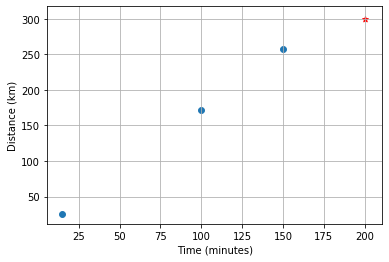
\includegraphics[width=0.7\textwidth]{interp_example1.png}
  \caption{An example of sampling of traveled distances at some time. The red point shows an additional sample taken after the trip velocity has been reduced.}
\end{figure}

Given two samples of the car traveled distance \(s_1\) and \(s_2\) taken at two different times \(t_1\) and \(t_2\) you can linearly interpolate to find your position at different times using the following relations:

\[s = (1 - w)\cdot s_1 + w \cdot s_2\]
where $t$ is a generic time at which we want to know the distance $s$ and \(w = \cfrac{t - t_1}{t_2 - t_1}\).

\subsubsection{Derivation}
The equation of a line for two points
\((t_1, s_1)\) and \((t_2, s_2)\) can be written as:

\[\frac{t - t_1}{t_2 - t_1} = \frac{s - s_1}{s_2 - s_1}\]

Setting \(w = \cfrac{t - t_1}{t_2 - t_1}\) and solving for \(s\) we find the desired solution:

\[(s_2 - s_1)\cdot w = s - s_1~~~\Rightarrow~~~s = (1 - w)\cdot s_1 + w \cdot s_2\]

This formula can also be understood as a weighted average where the weights are inversely related to the distance from the end points to the unknown point ($w_1 = (1 - w) = \cfrac{t_2 - t}{t_2 -t_1}, w_2 = w$), the closer point has more influence than the farther point.

Back to our example, if
\(s_1 = 25.75~\mathrm{km}\;(@t_1 = 15~\mathrm{min})\) and
\(s_2 = 171.7~\mathrm{km}\;(@t_2 = 100~\mathrm{min})\) let's find distance traveled in 1 hour (interpolation):

\begin{tcolorbox}[breakable, size=fbox, boxrule=1pt, pad at break*=1mm,colback=cellbackground, colframe=cellborder]
\begin{Verbatim}[commandchars=\\\{\}]
\PY{n}{s\PYZus{}1} \PY{o}{=} \PY{l+m+mf}{25.75} \PY{c+c1}{\PYZsh{} distance in km}
\PY{n}{t\PYZus{}1} \PY{o}{=} \PY{l+m+mi}{15}    \PY{c+c1}{\PYZsh{} elapsed time in minutes}
\PY{n}{s\PYZus{}2} \PY{o}{=} \PY{l+m+mf}{171.7}
\PY{n}{t\PYZus{}2} \PY{o}{=} \PY{l+m+mi}{100}

\PY{n}{t} \PY{o}{=} \PY{l+m+mi}{60}

\PY{n}{w} \PY{o}{=} \PY{p}{(}\PY{n}{t} \PY{o}{\PYZhy{}} \PY{n}{t\PYZus{}1}\PY{p}{)}\PY{o}{/}\PY{p}{(}\PY{n}{t\PYZus{}2} \PY{o}{\PYZhy{}} \PY{n}{t\PYZus{}1}\PY{p}{)}
\PY{n}{s} \PY{o}{=} \PY{p}{(}\PY{l+m+mi}{1} \PY{o}{\PYZhy{}} \PY{n}{w}\PY{p}{)}\PY{o}{*}\PY{n}{s\PYZus{}1} \PY{o}{+} \PY{n}{w}\PY{o}{*}\PY{n}{s\PYZus{}2}

\PY{n+nb}{print} \PY{p}{(}\PY{l+s+s2}{\PYZdq{}}\PY{l+s+si}{\PYZob{}:.1f\PYZcb{}}\PY{l+s+s2}{ km}\PY{l+s+s2}{\PYZdq{}}\PY{o}{.}\PY{n}{format}\PY{p}{(}\PY{n}{s}\PY{p}{)}\PY{p}{)}

103.0 km
\end{Verbatim}
\end{tcolorbox}

Always interpret critically your results to guess if they make sense or not. In the previous example we certainly expected something between 25.75 and 171.7~km (our range ends) furthermore since we are looking for the distance at a time which is almost halfway the interval, the result will be somehow in the middle or around 98.6~km. This is indeed more or less what we have got.
This simple reasoning should be applied every time you have a result to quickly judge it.

If we believe the relation between our variable stays the same ($f(t)$ still linear), we can use the same formula to \emph{extrapolate} values \emph{outside} our initial sample. For example if we keep the same constant velocity in our trip we could check the distance traveled after 3 hours:

\begin{tcolorbox}[breakable, size=fbox, boxrule=1pt, pad at break*=1mm,colback=cellbackground, colframe=cellborder]
\begin{Verbatim}[commandchars=\\\{\}]
\PY{n}{s\PYZus{}1} \PY{o}{=} \PY{l+m+mf}{25.75} \PY{c+c1}{\PYZsh{} distance in km}
\PY{n}{t\PYZus{}1} \PY{o}{=} \PY{l+m+mi}{15}    \PY{c+c1}{\PYZsh{} elapsed time in minutes}
\PY{n}{s\PYZus{}2} \PY{o}{=} \PY{l+m+mf}{171.7}
\PY{n}{t\PYZus{}2} \PY{o}{=} \PY{l+m+mi}{100}

\PY{n}{t} \PY{o}{=} \PY{l+m+mi}{180}

\PY{n}{w} \PY{o}{=} \PY{p}{(}\PY{n}{t} \PY{o}{\PYZhy{}} \PY{n}{t\PYZus{}1}\PY{p}{)}\PY{o}{/}\PY{p}{(}\PY{n}{t\PYZus{}2} \PY{o}{\PYZhy{}} \PY{n}{t\PYZus{}1}\PY{p}{)}
\PY{n}{s} \PY{o}{=} \PY{p}{(}\PY{l+m+mi}{1} \PY{o}{\PYZhy{}} \PY{n}{w}\PY{p}{)}\PY{o}{*}\PY{n}{s\PYZus{}1} \PY{o}{+} \PY{n}{w}\PY{o}{*}\PY{n}{s\PYZus{}2}

\PY{n+nb}{print} \PY{p}{(}\PY{l+s+s2}{\PYZdq{}}\PY{l+s+si}{\PYZob{}:.1f\PYZcb{}}\PY{l+s+s2}{ km}\PY{l+s+s2}{\PYZdq{}}\PY{o}{.}\PY{n}{format}\PY{p}{(}\PY{n}{s}\PY{p}{)}\PY{p}{)}

309.1 km
\end{Verbatim}
\end{tcolorbox}

\subsection{Log-linear interpolation}\label{log-linear-interpolation}
When the function $f$ that we want to interpolate is an exponential we can fall back to the previous case by a simple variable transformation. 
Assume the following is the relationship between $p$ and $h$, two generic variables:

\[p = \mathrm{exp}(c \cdot h)\]

Applying the logarithm to both sides of the equation gives:

\[s = \mathrm{log}(p) = \mathrm{log}(\mathrm{exp}(c \cdot h)) = c \cdot h\]
so there is linear relation between the new variable $s$ and $h$. At this point we can use the results of the previous section to interpolate for values of $s$, just remember to exponentiate the result to get the correct $p$. In formulas:

\[w = \frac{h - h_1}{h_2 - h_1}\]

\[s = (1 - w)\cdot s_1 + w \cdot s_2\;\;(\mathrm{remember \;now }\;s = \mathrm{log}(p))\]

\[p = \mathrm{exp}(s)\]

Atmospheric pressure decreases with the altitude (i.e.~the highest you flight the lower is the pressure) following an exponential law:

\[p = p_0\cdot e^{-\alpha h}\]
where
\begin{itemize}
\tightlist
\item
  \(h\) is the altitude
\item
  \(p_0\) is the pressure at sea level
\item
  \(\alpha\) is a constant
\end{itemize}

Taking the logarithm of each side of the equation I get a linear relation which can be interpolated as seen before:

\[s = \mathrm{log}(p) = \mathrm{log}(p_0\cdot e^{-\alpha h})\propto - \alpha \cdot h\]

Now assume that we have measured
\(p_1 = 90~\mathrm{kPa}\;(h_1 = 1000~\mathrm{m})\) and
\(p_2 = 40~\mathrm{kPa}\;(h_1 = 7000~\mathrm{m})\) what will be the
atmospheric pressure on top of the Mont Blanc (\(4812~\mathrm{m}\)) ? and on top of Mount Everest (\(8848~\mathrm{m}\)) ?

\begin{tcolorbox}[breakable, size=fbox, boxrule=1pt, pad at break*=1mm,colback=cellbackground, colframe=cellborder]
\begin{Verbatim}[commandchars=\\\{\}]
\PY{c+c1}{\PYZsh{} pressure on top of the Mont Blanc (interpolation)}
\PY{k+kn}{from} \PY{n+nn}{math} \PY{k}{import} \PY{n}{log}\PY{p}{,} \PY{n}{exp}

\PY{c+c1}{\PYZsh{} first we take the logarithm of our measurements to use the linear }
\PY{c+c1}{\PYZsh{} relation to interpolate}
\PY{n}{h\PYZus{}1} \PY{o}{=} \PY{l+m+mi}{1000} \PY{c+c1}{\PYZsh{} height in meters}
\PY{n}{s\PYZus{}1} \PY{o}{=} \PY{n}{log}\PY{p}{(}\PY{l+m+mi}{90}\PY{p}{)} \PY{c+c1}{\PYZsh{} logarithm of the pressure at heigth h1}
\PY{n}{h\PYZus{}2} \PY{o}{=} \PY{l+m+mi}{7000} \PY{c+c1}{\PYZsh{} height in meters}
\PY{n}{s\PYZus{}2} \PY{o}{=} \PY{n}{log}\PY{p}{(}\PY{l+m+mi}{40}\PY{p}{)} \PY{c+c1}{\PYZsh{} logarithm of the pressure at heigth h2}

\PY{n}{h} \PY{o}{=} \PY{l+m+mi}{4812}

\PY{n}{w} \PY{o}{=} \PY{p}{(}\PY{n}{h} \PY{o}{\PYZhy{}} \PY{n}{h\PYZus{}1}\PY{p}{)}\PY{o}{/}\PY{p}{(}\PY{n}{h\PYZus{}2} \PY{o}{\PYZhy{}} \PY{n}{h\PYZus{}1}\PY{p}{)}
\PY{n}{s} \PY{o}{=} \PY{p}{(}\PY{l+m+mi}{1} \PY{o}{\PYZhy{}} \PY{n}{w}\PY{p}{)}\PY{o}{*}\PY{n}{s\PYZus{}1} \PY{o}{+} \PY{n}{w}\PY{o}{*}\PY{n}{s\PYZus{}2}

\PY{n+nb}{print} \PY{p}{(}\PY{l+s+s2}{\PYZdq{}}\PY{l+s+si}{\PYZob{}:.1f\PYZcb{}}\PY{l+s+s2}{ kPa}\PY{l+s+s2}{\PYZdq{}}\PY{o}{.}\PY{n}{format}\PY{p}{(}\PY{n}{exp}\PY{p}{(}\PY{n}{s}\PY{p}{)}\PY{p}{)}\PY{p}{)}

53.8 kPa
\end{Verbatim}
\end{tcolorbox}

\begin{tcolorbox}[breakable, size=fbox, boxrule=1pt, pad at break*=1mm,colback=cellbackground, colframe=cellborder]
\begin{Verbatim}[commandchars=\\\{\}]
\PY{c+c1}{\PYZsh{} pressure on top of the Mount Everest (extrapolation)}
\PY{k+kn}{from} \PY{n+nn}{math} \PY{k}{import} \PY{n}{log}\PY{p}{,} \PY{n}{exp}

\PY{c+c1}{\PYZsh{} first we take the logarithm of our measurements to use the linear }
\PY{c+c1}{\PYZsh{} relation to interpolate}
\PY{n}{h\PYZus{}1} \PY{o}{=} \PY{l+m+mi}{1000} \PY{c+c1}{\PYZsh{} height in meters}
\PY{n}{s\PYZus{}1} \PY{o}{=} \PY{n}{log}\PY{p}{(}\PY{l+m+mi}{90}\PY{p}{)} \PY{c+c1}{\PYZsh{} logarithm of the pressure at heigth h1}
\PY{n}{h\PYZus{}2} \PY{o}{=} \PY{l+m+mi}{7000} \PY{c+c1}{\PYZsh{} height in meters}
\PY{n}{s\PYZus{}2} \PY{o}{=} \PY{n}{log}\PY{p}{(}\PY{l+m+mi}{40}\PY{p}{)} \PY{c+c1}{\PYZsh{} logarithm of the pressure at heigth h2}
\PY{n}{h} \PY{o}{=} \PY{l+m+mi}{8848}

\PY{n}{w} \PY{o}{=} \PY{p}{(}\PY{n}{h} \PY{o}{\PYZhy{}} \PY{n}{h\PYZus{}1}\PY{p}{)}\PY{o}{/}\PY{p}{(}\PY{n}{h\PYZus{}2} \PY{o}{\PYZhy{}} \PY{n}{h\PYZus{}1}\PY{p}{)}
\PY{n}{s} \PY{o}{=} \PY{p}{(}\PY{l+m+mi}{1} \PY{o}{\PYZhy{}} \PY{n}{w}\PY{p}{)}\PY{o}{*}\PY{n}{s\PYZus{}1} \PY{o}{+} \PY{n}{w}\PY{o}{*}\PY{n}{s\PYZus{}2}

\PY{n+nb}{print} \PY{p}{(}\PY{l+s+s2}{\PYZdq{}}\PY{l+s+si}{\PYZob{}:.1f\PYZcb{}}\PY{l+s+s2}{ kPa}\PY{l+s+s2}{\PYZdq{}}\PY{o}{.}\PY{n}{format}\PY{p}{(}\PY{n}{exp}\PY{p}{(}\PY{n}{s}\PY{p}{)}\PY{p}{)}\PY{p}{)}

31.2 kPa
\end{Verbatim}
\end{tcolorbox}

\begin{figure}
\centering
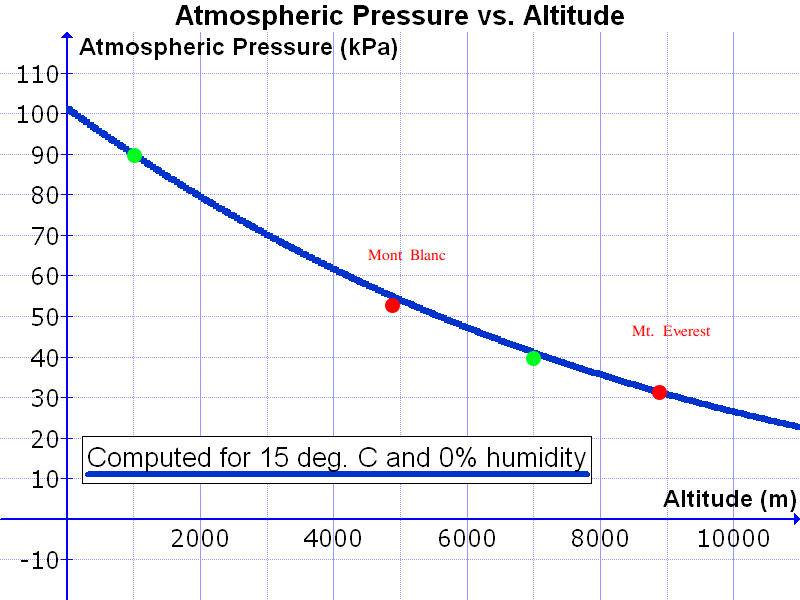
\includegraphics[width=0.7\linewidth]{Atmospheric_Pressure_vs._Altitude.png}
\caption{Atmospheric pressure versus altitude (Wikipedia). Green points
represent our measurements, red points represent
interpolation/extrapolation.}
\end{figure}

\subsection{Limitations of Interpolation}
Interpolation is just an approximation and works well when either the function $f$ is linear or we are trying to interpolate between two points that are close enough to believe that $f$ is almost linear in that interval.

It can be easily demonstrated that the linear approximation between two points of a given function $f(x)$ gets worse with the second derivative of the function that is approximated ($f''(x)$). This is intuitively correct: the "curvier" the function is, the worse the approximation made with simple linear interpolation becomes, see Fig.~\ref{fig:sine_interp}.

\begin{figure}
  \centering
  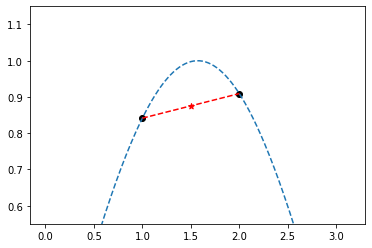
\includegraphics[width=0.7\textwidth]{wrong_interp.png}
  \caption{Trying to approximate a sine function with a line is clearly not going to work unless the interpolation interval is very small.}
  \label{fig:sine_interp}
\end{figure}

To improve the approximation accuracy with complicated curves a polynomial of higher order can be used ($𝑝(𝑥)=𝑎_0 + 𝑎_1 𝑥+ 𝑎_2 𝑥^2+\cdots$), for example in the evaluation of the natural logarithm and trigonometric functions. It has to be clear however that going to higher degrees does not always help (for those interested \href{https://en.wikipedia.org/wiki/Runge%27s_phenomenon}{see Runge's phenomenon}).

\section{Discount curve interpolation}\label{discount-curve-interpolation}

Finally we can come back to finance. Since discount factors are derived from a discrete set of dates we may need to find the factor at some different date and clearly we can use interpolation to do it.
Now we will see how to implement a \texttt{python} function which interpolates some given discount factors.
Needed data:

\begin{itemize}
\tightlist
\item a list of pillars dates specifying the value dates of the given discount factors, \(t_0,...,t_{n-1}\);
\item a list of given discount factors, \(D(t_0),...,D(t_{n-1})\);
\item a pricing date (`today' date) which corresponds to \(t=0\).
\end{itemize}

The input argument to the function will be the value date at which we want to interpolate the discount factor. Since the discount factor can be expressed as \(D=e^{-r(T-t)}\) the function will use a log-linear interpolation to return the value at a date not included in the given pillars.
More technically we can say that we are doing a linear interpolation over time in the log space:

\[d(t_i):=\mathrm{ln}(D(t_i))\]

\[d(t) = (1-w)d(t_i) + wd(t_{i+1});\;\;\;w=\frac{t-t_i}{t_{i+1}-t_i}\]

\[D(t) = \mathrm{exp}(d(t))\]
where again \(i\) is such that \(t_i \le t \le t_{i+1}\)

This time instead of reinventing the wheel and performing the interpolation with our own code, we'll use the function \texttt{interp} provided by the module \texttt{numpy}; this function linearly interpolates between the provided points to estimate the value of $f$ at some "new" $x$.
Say we want to interpolate the points at $x = 2.5$ given the following values:

\begin{tcolorbox}[breakable, size=fbox, boxrule=1pt, pad at break*=1mm,colback=cellbackground, colframe=cellborder]
\begin{Verbatim}[commandchars=\\\{\}]
\PY{k+kn}{import} \PY{n+nn}{numpy} \PY{k}{as} \PY{n+nn}{np}

\PY{n}{xp} \PY{o}{=} \PY{p}{[}\PY{l+m+mi}{0}\PY{p}{,} \PY{l+m+mi}{1}\PY{p}{,} \PY{l+m+mi}{5}\PY{p}{]}
\PY{n}{fp} \PY{o}{=} \PY{p}{[}\PY{l+m+mi}{0}\PY{p}{,} \PY{l+m+mi}{2}\PY{p}{,} \PY{l+m+mi}{4}\PY{p}{]}
\PY{n}{np}\PY{o}{.}\PY{n}{interp}\PY{p}{(}\PY{l+m+mf}{2.5}\PY{p}{,} \PY{n}{xp}\PY{p}{,} \PY{n}{fp}\PY{p}{)}

2.75
\end{Verbatim}
\end{tcolorbox}

Assume we have three discount factors instead:
\begin{tcolorbox}[breakable, size=fbox, boxrule=1pt, pad at break*=1mm,colback=cellbackground, colframe=cellborder]
\begin{Verbatim}[commandchars=\\\{\}]
\PY{c+c1}{\PYZsh{} import modules and objects that we need}
\PY{k+kn}{from} \PY{n+nn}{datetime} \PY{k}{import} \PY{n}{date}
\PY{k+kn}{import} \PY{n+nn}{numpy}\PY{o}{,} \PY{n+nn}{math}
\PY{k+kn}{from} \PY{n+nn}{matplotlib} \PY{k}{import} \PY{n}{pyplot} \PY{k}{as} \PY{n}{plt}
\PY{k+kn}{import} \PY{n+nn}{matplotlib}\PY{n+nn}{.}\PY{n+nn}{dates} \PY{k}{as} \PY{n+nn}{mdates} 
\PY{c+c1}{\PYZsh{} with this notation we tell python to use mdates as an alias }
\PY{c+c1}{\PYZsh{} for matplotlib.dates}

\PY{c+c1}{\PYZsh{} define the input data}
\PY{n}{today\PYZus{}date} \PY{o}{=} \PY{n}{date}\PY{p}{(}\PY{l+m+mi}{2019}\PY{p}{,} \PY{l+m+mi}{10}\PY{p}{,} \PY{l+m+mi}{1}\PY{p}{)}

\PY{n}{pillar\PYZus{}dates} \PY{o}{=} \PY{p}{[}\PY{n}{date}\PY{p}{(}\PY{l+m+mi}{2019}\PY{p}{,} \PY{l+m+mi}{10}\PY{p}{,} \PY{l+m+mi}{1}\PY{p}{)}\PY{p}{,} \PY{n}{date}\PY{p}{(}\PY{l+m+mi}{2020}\PY{p}{,} \PY{l+m+mi}{10}\PY{p}{,} \PY{l+m+mi}{1}\PY{p}{)}\PY{p}{,} \PY{n}{date}\PY{p}{(}\PY{l+m+mi}{2021}\PY{p}{,} \PY{l+m+mi}{10}\PY{p}{,} \PY{l+m+mi}{1}\PY{p}{)}\PY{p}{]}
\PY{n}{discount\PYZus{}factors} \PY{o}{=} \PY{p}{[}\PY{l+m+mf}{1.0}\PY{p}{,} \PY{l+m+mf}{0.97}\PY{p}{,} \PY{l+m+mf}{0.72}\PY{p}{]}
\end{Verbatim}
\end{tcolorbox}
    
Let's see what this fake discount curve looks like when plotted on a graph:

\begin{tcolorbox}[breakable, size=fbox, boxrule=1pt, pad at break*=1mm,colback=cellbackground, colframe=cellborder]
\begin{Verbatim}[commandchars=\\\{\}]
\PY{n}{plt}\PY{o}{.}\PY{n}{plot}\PY{p}{(}\PY{n}{pillar\PYZus{}dates}\PY{p}{,} \PY{n}{discount\PYZus{}factors}\PY{p}{,} \PY{n}{marker}\PY{o}{=}\PY{l+s+s1}{\PYZsq{}}\PY{l+s+s1}{o}\PY{l+s+s1}{\PYZsq{}}\PY{p}{)}
\PY{n}{plt}\PY{o}{.}\PY{n}{gca}\PY{p}{(}\PY{p}{)}\PY{o}{.}\PY{n}{xaxis}\PY{o}{.}\PY{n}{set\PYZus{}major\PYZus{}formatter}\PY{p}{(}\PY{n}{mdates}\PY{o}{.}\PY{n}{DateFormatter}\PY{p}{(}\PY{l+s+s1}{\PYZsq{}}\PY{l+s+s1}{\PYZpc{}}\PY{l+s+s1}{m/}\PY{l+s+si}{\PYZpc{}d}\PY{l+s+s1}{/}\PY{l+s+s1}{\PYZpc{}}\PY{l+s+s1}{Y}\PY{l+s+s1}{\PYZsq{}}\PY{p}{)}\PY{p}{)}
\PY{n}{plt}\PY{o}{.}\PY{n}{gca}\PY{p}{(}\PY{p}{)}\PY{o}{.}\PY{n}{xaxis}\PY{o}{.}\PY{n}{set\PYZus{}major\PYZus{}locator}\PY{p}{(}\PY{n}{mdates}\PY{o}{.}\PY{n}{YearLocator}\PY{p}{(}\PY{p}{)}\PY{p}{)}
\PY{n}{plt}\PY{o}{.}\PY{n}{grid}\PY{p}{(}\PY{k+kc}{True}\PY{p}{)}
\PY{n}{plt}\PY{o}{.}\PY{n}{show}\PY{p}{(}\PY{p}{)}
\end{Verbatim}
\end{tcolorbox}
\vfill
\begin{figure}[h]
  \centering
  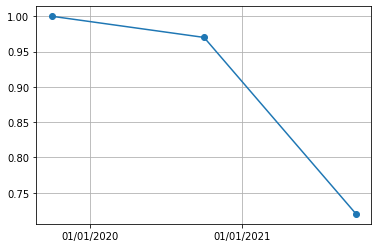
\includegraphics[width=0.7\textwidth]{lecture_3_10_0.png}
\end{figure}
    
Since it is a computation that from now on we need to perform quite often it is convenient to write a function that compute the discount factor at arbitrary dates.

\begin{tcolorbox}[breakable, size=fbox, boxrule=1pt, pad at break*=1mm,colback=cellbackground, colframe=cellborder]
\begin{Verbatim}[commandchars=\\\{\}]
\PY{c+c1}{\PYZsh{} define the df function}
\PY{k}{def} \PY{n+nf}{df}\PY{p}{(}\PY{n}{d, pillar_dates, discount_factors}\PY{p}{)}\PY{p}{:}
    \PY{c+c1}{\PYZsh{} first thing we need to do is to apply the logarithm function}
    \PY{c+c1}{\PYZsh{} to the discount factors since we are doing log-linear and}
    \PY{c+c1}{\PYZsh{} not just linear interpolation}
    \PY{n}{log\PYZus{}discount\PYZus{}factors} \PY{o}{=} \PY{p}{[}\PY{p}{]}
    \PY{k}{for} \PY{n}{discount\PYZus{}factor} \PY{o+ow}{in} \PY{n}{discount\PYZus{}factors}\PY{p}{:}
        \PY{n}{log\PYZus{}discount\PYZus{}factors}\PY{o}{.}\PY{n}{append}\PY{p}{(}\PY{n}{math}\PY{o}{.}\PY{n}{log}\PY{p}{(}\PY{n}{discount\PYZus{}factor}\PY{p}{)}\PY{p}{)}
    
    \PY{c+c1}{\PYZsh{} perform the linear interpolation of the log discount factors}
    \PY{n}{interpolated\PYZus{}log\PYZus{}discount\PYZus{}factor} \PY{o}{=} \PYZbs{}
        \PY{n}{numpy}\PY{o}{.}\PY{n}{interp}\PY{p}{(}\PY{n}{d}\PY{p}{,} \PY{n}{pillar\PYZus{}dates}\PY{p}{,} \PY{n}{log\PYZus{}discount\PYZus{}factors}\PY{p}{)}
    
    \PY{c+c1}{\PYZsh{} return the interpolated discount factor}
    \PY{k}{return} \PY{n}{math}\PY{o}{.}\PY{n}{exp}\PY{p}{(}\PY{n}{interpolated\PYZus{}log\PYZus{}discount\PYZus{}factor}\PY{p}{)}
\end{Verbatim}
\end{tcolorbox}

This is almost OK, \textbf{but it won't work} because \texttt{numpy.interp} only accepts numbers or a list of numbers as argument i.e.~it doesn't automatically convert or interpret dates as numbers so doesn't know how to interpolate them. So we need to do the conversion ourselves before passing the dates into the interpolation function.
The following updated version of our function converts the pillar dates into ``pillar days'' i.e. each date is replaced by the number of days today ($t_0$):

\begin{tcolorbox}[breakable, size=fbox, boxrule=1pt, pad at break*=1mm,colback=cellbackground, colframe=cellborder]
\begin{Verbatim}[commandchars=\\\{\}]
\PY{k}{def} \PY{n+nf}{df}\PY{p}{(}\PY{n}{d, today_date, pillar_dates, discount_factors}\PY{p}{)}\PY{p}{:}
    \PY{c+c1}{\PYZsh{} first thing we need to do is to apply the logarithm function}
    \PY{c+c1}{\PYZsh{} to the discount factors since we are doing log-linear and}
    \PY{c+c1}{\PYZsh{} not just linear interpolation}
    \PY{n}{log\PYZus{}discount\PYZus{}factors} \PY{o}{=} \PY{p}{[}\PY{p}{]}
    \PY{k}{for} \PY{n}{discount\PYZus{}factor} \PY{o+ow}{in} \PY{n}{discount\PYZus{}factors}\PY{p}{:}
        \PY{n}{log\PYZus{}discount\PYZus{}factors}\PY{o}{.}\PY{n}{append}\PY{p}{(}\PY{n}{math}\PY{o}{.}\PY{n}{log}\PY{p}{(}\PY{n}{discount\PYZus{}factor}\PY{p}{)}\PY{p}{)}
    
    \PY{c+c1}{\PYZsh{} convert the pillar dates to pillar \PYZsq{}days\PYZsq{}}
    \PY{c+c1}{\PYZsh{} i.e. number of days from today}
    \PY{c+c1}{\PYZsh{} to write shorter code we can use this NEW notation}
    \PY{c+c1}{\PYZsh{} which condenses for and list creation in one line}
    \PY{n}{pillar\PYZus{}days} \PY{o}{=} \PYZbs{}
        \PY{p}{[}\PY{p}{(}\PY{n}{pillar\PYZus{}date} \PY{o}{\PYZhy{}} \PY{n}{today\PYZus{}date}\PY{p}{)}\PY{o}{.}\PY{n}{days} \PY{k}{for} \PY{n}{pillar\PYZus{}date} \PY{o+ow}{in} \PY{n}{pillar\PYZus{}dates}\PY{p}{]}
    
    \PY{c+c1}{\PYZsh{} obviously we need to do the same to the value date}
    \PY{c+c1}{\PYZsh{} argument of the df function}
    \PY{n}{d\PYZus{}days} \PY{o}{=} \PY{p}{(}\PY{n}{d} \PY{o}{\PYZhy{}} \PY{n}{today\PYZus{}date}\PY{p}{)}\PY{o}{.}\PY{n}{days}
    
    \PY{c+c1}{\PYZsh{} perform the linear interpolation of the log discount factors}
    \PY{n}{interpolated\PYZus{}log\PYZus{}discount\PYZus{}factor} \PY{o}{=} \PYZbs{}
        \PY{n}{numpy}\PY{o}{.}\PY{n}{interp}\PY{p}{(}\PY{n}{d\PYZus{}days}\PY{p}{,} \PY{n}{pillar\PYZus{}days}\PY{p}{,} \PY{n}{log\PYZus{}discount\PYZus{}factors}\PY{p}{)}
    
    \PY{c+c1}{\PYZsh{} return the interpolated discount factor}
    \PY{k}{return} \PY{n}{math}\PY{o}{.}\PY{n}{exp}\PY{p}{(}\PY{n}{interpolated\PYZus{}log\PYZus{}discount\PYZus{}factor}\PY{p}{)}
\end{Verbatim}
\end{tcolorbox}

Now we can use the \texttt{df} function to get discount factors on value dates between the given pillar dates:

\begin{tcolorbox}[breakable, size=fbox, boxrule=1pt, pad at break*=1mm,colback=cellbackground, colframe=cellborder]
\begin{Verbatim}[commandchars=\\\{\}]
\PY{n}{d0} \PY{o}{=} \PY{n}{date}\PY{p}{(}\PY{l+m+mi}{2020}\PY{p}{,} \PY{l+m+mi}{1}\PY{p}{,} \PY{l+m+mi}{1}\PY{p}{)}
\PY{n}{df0} \PY{o}{=} \PY{n}{df}\PY{p}{(}\PY{n}{d0, today_date, pillar_dates, discount_factors}\PY{p}{)}
\PY{n+nb}{print} \PY{p}{(}\PY{n}{df0}\PY{p}{)}

0.9923728228571693
\end{Verbatim}
\end{tcolorbox}

\begin{tcolorbox}[breakable, size=fbox, boxrule=1pt, pad at break*=1mm,colback=cellbackground, colframe=cellborder]
\begin{Verbatim}[commandchars=\\\{\}]
\PY{n}{d1} \PY{o}{=} \PY{n}{date}\PY{p}{(}\PY{l+m+mi}{2021}\PY{p}{,} \PY{l+m+mi}{1}\PY{p}{,} \PY{l+m+mi}{1}\PY{p}{)}
\PY{n}{df1} \PY{o}{=} \PY{n}{df}\PY{p}{(}\PY{n}{d1, today_date, pillar_dates, discount_factors}\PY{p}{)}
\PY{n+nb}{print} \PY{p}{(}\PY{n}{df1}\PY{p}{)}

0.8997999273630835
\end{Verbatim}
\end{tcolorbox}

Another very useful way to check the correctness of a result is by plotting data, so let's see what these look like when plotted on a semi-log graph and if they make sense:
    
\begin{tcolorbox}[breakable, size=fbox, boxrule=1pt, pad at break*=1mm,colback=cellbackground, colframe=cellborder]
\begin{Verbatim}[commandchars=\\\{\}]
\PY{k+kn}{from} \PY{n+nn}{matplotlib} \PY{k}{import} \PY{n}{pyplot} \PY{k}{as} \PY{n}{plt}
\PY{k+kn}{import} \PY{n+nn}{matplotlib}\PY{n+nn}{.}\PY{n+nn}{dates} \PY{k}{as} \PY{n+nn}{mdates}

\PY{n}{plt}\PY{o}{.}\PY{n}{semilogy}\PY{p}{(}\PY{n}{pillar\PYZus{}dates}\PY{p}{,} \PY{n}{discount\PYZus{}factors}\PY{p}{,} \PY{n}{marker}\PY{o}{=}\PY{l+s+s1}{\PYZsq{}}\PY{l+s+s1}{o}\PY{l+s+s1}{\PYZsq{}}\PY{p}{)}
\PY{n}{plt}\PY{o}{.}\PY{n}{semilogy}\PY{p}{(}\PY{n}{d0}\PY{p}{,}\PY{n}{df0} \PY{p}{,} \PY{n}{marker}\PY{o}{=}\PY{l+s+s1}{\PYZsq{}}\PY{l+s+s1}{X}\PY{l+s+s1}{\PYZsq{}}\PY{p}{)}
\PY{n}{plt}\PY{o}{.}\PY{n}{semilogy}\PY{p}{(}\PY{n}{d1}\PY{p}{,}\PY{n}{df1} \PY{p}{,} \PY{n}{marker}\PY{o}{=}\PY{l+s+s1}{\PYZsq{}}\PY{l+s+s1}{X}\PY{l+s+s1}{\PYZsq{}}\PY{p}{)}
\PY{n}{plt}\PY{o}{.}\PY{n}{gca}\PY{p}{(}\PY{p}{)}\PY{o}{.}\PY{n}{xaxis}\PY{o}{.}\PY{n}{set\PYZus{}major\PYZus{}formatter}\PY{p}{(}\PY{n}{mdates}\PY{o}{.}\PY{n}{DateFormatter}\PY{p}{(}\PY{l+s+s1}{\PYZsq{}}\PY{l+s+s1}{\PYZpc{}}\PY{l+s+s1}{m/}\PY{l+s+si}{\PYZpc{}d}\PY{l+s+s1}{/}\PY{l+s+s1}{\PYZpc{}}\PY{l+s+s1}{Y}\PY{l+s+s1}{\PYZsq{}}\PY{p}{)}\PY{p}{)}
\PY{n}{plt}\PY{o}{.}\PY{n}{gca}\PY{p}{(}\PY{p}{)}\PY{o}{.}\PY{n}{xaxis}\PY{o}{.}\PY{n}{set\PYZus{}major\PYZus{}locator}\PY{p}{(}\PY{n}{mdates}\PY{o}{.}\PY{n}{YearLocator}\PY{p}{(}\PY{p}{)}\PY{p}{)}
\PY{n}{plt}\PY{o}{.}\PY{n}{grid}\PY{p}{(}\PY{k+kc}{True}\PY{p}{)}
\PY{n}{plt}\PY{o}{.}\PY{n}{show}\PY{p}{(}\PY{p}{)}
\end{Verbatim}
\end{tcolorbox}
\vfill
\begin{figure}[h]
  \centering
  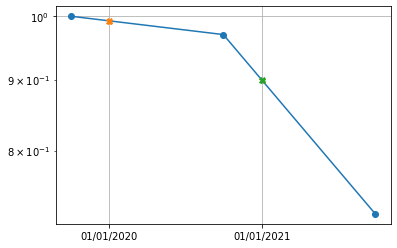
\includegraphics[width=0.7\textwidth]{lecture_3_15_0.png}
\end{figure}

Let's see what these look like when plotted on a linear graph instead:
    
\begin{tcolorbox}[breakable, size=fbox, boxrule=1pt, pad at break*=1mm,colback=cellbackground, colframe=cellborder]
\begin{Verbatim}[commandchars=\\\{\}]
\PY{k+kn}{from} \PY{n+nn}{matplotlib} \PY{k}{import} \PY{n}{pyplot} \PY{k}{as} \PY{n}{plt}
\PY{k+kn}{import} \PY{n+nn}{matplotlib}\PY{n+nn}{.}\PY{n+nn}{dates} \PY{k}{as} \PY{n+nn}{mdates}
\PY{n}{plt}\PY{o}{.}\PY{n}{plot}\PY{p}{(}\PY{n}{pillar\PYZus{}dates}\PY{p}{,} \PY{n}{discount\PYZus{}factors}\PY{p}{,} \PY{n}{marker}\PY{o}{=}\PY{l+s+s1}{\PYZsq{}}\PY{l+s+s1}{o}\PY{l+s+s1}{\PYZsq{}}\PY{p}{)}
\PY{n}{plt}\PY{o}{.}\PY{n}{plot}\PY{p}{(}\PY{n}{d0}\PY{p}{,}\PY{n}{df0} \PY{p}{,} \PY{n}{marker}\PY{o}{=}\PY{l+s+s1}{\PYZsq{}}\PY{l+s+s1}{X}\PY{l+s+s1}{\PYZsq{}}\PY{p}{)}
\PY{n}{plt}\PY{o}{.}\PY{n}{plot}\PY{p}{(}\PY{n}{d1}\PY{p}{,}\PY{n}{df1} \PY{p}{,} \PY{n}{marker}\PY{o}{=}\PY{l+s+s1}{\PYZsq{}}\PY{l+s+s1}{X}\PY{l+s+s1}{\PYZsq{}}\PY{p}{)}
\PY{n}{plt}\PY{o}{.}\PY{n}{gca}\PY{p}{(}\PY{p}{)}\PY{o}{.}\PY{n}{xaxis}\PY{o}{.}\PY{n}{set\PYZus{}major\PYZus{}formatter}\PY{p}{(}\PY{n}{mdates}\PY{o}{.}\PY{n}{DateFormatter}\PY{p}{(}\PY{l+s+s1}{\PYZsq{}}\PY{l+s+s1}{\PYZpc{}}\PY{l+s+s1}{m/}\PY{l+s+si}{\PYZpc{}d}\PY{l+s+s1}{/}\PY{l+s+s1}{\PYZpc{}}\PY{l+s+s1}{Y}\PY{l+s+s1}{\PYZsq{}}\PY{p}{)}\PY{p}{)}
\PY{n}{plt}\PY{o}{.}\PY{n}{gca}\PY{p}{(}\PY{p}{)}\PY{o}{.}\PY{n}{xaxis}\PY{o}{.}\PY{n}{set\PYZus{}major\PYZus{}locator}\PY{p}{(}\PY{n}{mdates}\PY{o}{.}\PY{n}{YearLocator}\PY{p}{(}\PY{p}{)}\PY{p}{)}
\PY{n}{plt}\PY{o}{.}\PY{n}{grid}\PY{p}{(}\PY{k+kc}{True}\PY{p}{)}
\PY{n}{plt}\PY{o}{.}\PY{n}{show}\PY{p}{(}\PY{p}{)}
\end{Verbatim}
\end{tcolorbox}
\vfill
\begin{figure}[h]
  \centering
  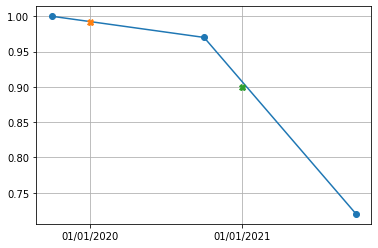
\includegraphics[width=0.7\textwidth]{lecture_3_16_0.png}
\end{figure}

Discrepancies in the linear plot are most likely due to rounding.

\section{Forward Rates}\label{calculating-forward-rates}

A forward rate is an interest rate applicable to a financial transaction that will take place in the future. Forward rates are calculated from the spot rate by exploiting the no arbitrage condition which states that investing at rate \(r_1\) for the period \((0, T_1)\) and then \emph{re-investing} at rate \(r_{1,2}\) for the time period \((T_1, T_2)\) is equivalent to invest at rate \(r_2\) for the full time period \((0, T_2)\). Essentially two investors shouldn't be able to earn money from arbitraging between different interest periods. That said:

\[(1+r_1 T_1)(1+r_{1,2}(T_2 - T_1)) = 1 + r_2 T_2\]

Solving for \(r_{1,2}\) leads to

\[F(T_1, T_2) = r_{1,2} = \frac{1}{T_2-T_1}\Big(\frac{D(T_1)}{D(T_2)} - 1 \Big)~~~~\textrm{(where $D{(T_i)}=\frac{1}{1+r_iT_{i}}$)}\]

\begin{tcolorbox}[breakable, size=fbox, boxrule=1pt, pad at break*=1mm,colback=cellbackground, colframe=cellborder]
\begin{Verbatim}[commandchars=\\\{\}]
\PY{k+kn}{from} \PY{n+nn}{datetime} \PY{k}{import} \PY{n}{date}
\PY{k+kn}{import} \PY{n+nn}{numpy}\PY{o}{,} \PY{n+nn}{math}

\PY{n}{today\PYZus{}date} \PY{o}{=} \PY{n}{date} \PY{p}{(}\PY{l+m+mi}{2019}\PY{p}{,} \PY{l+m+mi}{1}\PY{p}{,} \PY{l+m+mi}{1}\PY{p}{)}

\PY{n}{pillar\PYZus{}dates} \PY{o}{=} \PY{p}{[}\PY{n}{date}\PY{p}{(}\PY{l+m+mi}{2019} \PY{p}{,} \PY{l+m+mi}{1} \PY{p}{,}\PY{l+m+mi}{1}\PY{p}{)}\PY{p}{,} 
                \PY{n}{date}\PY{p}{(}\PY{l+m+mi}{2020}\PY{p}{,} \PY{l+m+mi}{1}\PY{p}{,} \PY{l+m+mi}{1}\PY{p}{)}\PY{p}{,} 
                \PY{n}{date}\PY{p}{(}\PY{l+m+mi}{2021}\PY{p}{,} \PY{l+m+mi}{10} \PY{p}{,}\PY{l+m+mi}{1}\PY{p}{)}\PY{p}{]}
\PY{n}{discount\PYZus{}factors} \PY{o}{=} \PY{p}{[}\PY{l+m+mf}{1.0}\PY{p}{,} \PY{l+m+mf}{0.97}\PY{p}{,} \PY{l+m+mf}{0.72}\PY{p}{]}

\PY{k}{def} \PY{n+nf}{forward\PYZus{}rate}\PY{p}{(}\PY{n}{t1}\PY{p}{,} \PY{n}{t2, today_date, pillar_dates, discount_factors}\PY{p}{)}\PY{p}{:}
    \PY{k}{return} \PY{l+m+mf}{365.0}\PY{o}{/}\PY{p}{(}\PY{n}{t2}\PY{o}{\PYZhy{}}\PY{n}{t1}\PY{p}{)}\PY{o}{.}\PY{n}{days} \PY{o}{*}
        \PY{p}{(}\PY{n}{df}\PY{p}{(}\PY{n}{t1, today_date, pillar_dates, discount_factors}\PY{p}{)} \PY{o}{/}
        \PY{n}{df}\PY{p}{(}\PY{n}{t2, today_date, pillar_dates, discount_factors}\PY{p}{)} \PY{o}{\PYZhy{}} \PY{l+m+mi}{1}\PY{p}{)}

\PY{n}{forward\PYZus{}rate}\PY{p}{(}\PY{n}{date}\PY{p}{(}\PY{l+m+mi}{2019}\PY{p}{,} \PY{l+m+mi}{2}\PY{p}{,} \PY{l+m+mi}{1}\PY{p}{)}\PY{p}{,} \PY{n}{date}\PY{p}{(}\PY{l+m+mi}{2019}\PY{p}{,} \PY{l+m+mi}{8}\PY{p}{,} \PY{l+m+mi}{1}\PY{p}{),}
             \PY{p}{today_date, pillar_dates, discount_factors}\PY{p}{)}
\end{Verbatim}
\end{tcolorbox}

\subsection{2008 Financial Crisis}\label{financial-crisis}

Looking at the historical series of the Euribor (6M) rate versus the Eonia Overnight Indexed Swap (OIS-6M) rate over the time interval 2006-2011 it becomes apparent how before August 2007 the two rates display strictly overlapping trends differing of no more than 6 bps.

\begin{figure}[h]
\centering
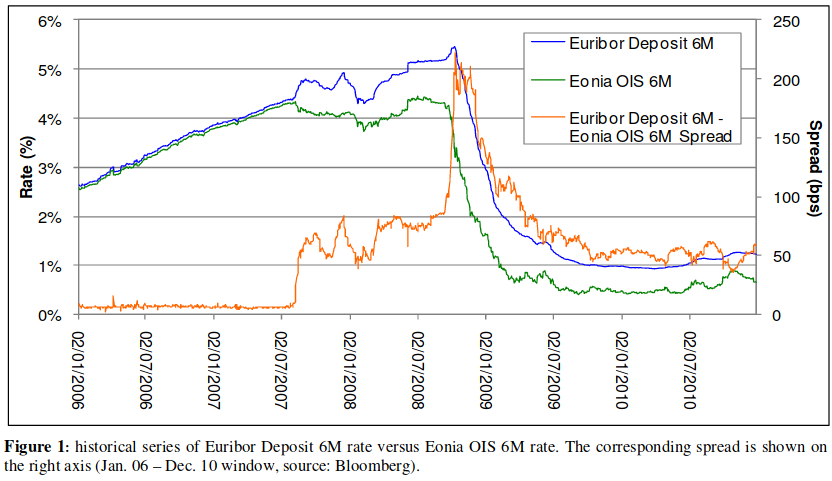
\includegraphics[width=0.7\linewidth]{credit_crunch.png}
\end{figure}

In August 2007 however we observe a sudden increase of the Euribor rate and a simultaneous decrease of the OIS rate that leads to the explosion of the corresponding basis spread, touching the peak of 222 bps in October 2008, when Lehman Brothers filed for bankruptcy. Successively the basis has sensibly reduced and stabilized between 40 bps and 60 bps (notice that the pre-crisis level has never been recovered). The same effect is observed for other similar couples of series, e.g.~Euribor 3M vs OIS 3M.

The reason of the abrupt divergence between the Euribor and OIS rates can be explained by considering both the monetary policy decisions adopted by international authorities in response to the financial turmoil, and the impact of the credit crunch on both credit and liquidity risk perception of the market, coupled with the different financial meaning and dynamics of these rates.

\begin{itemize}
\tightlist
\item
  The Euribor rate is the reference rate for over-the-counter (OTC)
  transactions in the Euro area. It is defined as the rate at which
  Euro inter-bank deposits are being offered within the EMU zone by one
  prime bank to another at 11:00 a.m. Brussels time. The rate fixings
  for a strip of 15 maturities (from one day to one year) are
  constructed as the average of the rates submitted (excluding the
  highest and lowest 15\% tails) by a panel of 42 banks, selected
  among the EU banks with the highest volume of business in the Euro
  zone money markets, plus some large international bank from non-EU
  countries with important euro zone operations. \emph{Thus, Euribor
  rates reflect the average cost of funding of banks in the inter bank
  market at each given maturity. During the crisis the solvency and
  solidity of the whole financial sector was brought into question and
  the credit and liquidity risk and uremia associated to inter-bank
  counter-parties sharply increased.} The Euribor rates immediately
  reflected these dynamics and raise to their highest values over more
  than 10 years. As seen in the plot above, the Euribor 6M rate suddenly
  increased on August 2007 and reached 5.49\% on 10th October 2008.
\item
  The Eonia rate is the reference rate for overnight OTC transactions in
  the Euro area. It is constructed as the average rate of the overnight
  transactions (one day maturity deposits) executed during a given
  business day by a panel of banks on the inter-bank money market,
  weighted with the corresponding transaction volumes. \emph{The Eonia
  Contribution Panel coincides with the Euribor Contribution Panel, thus
  Eonia rate includes information on the short term (overnight)
  liquidity expectations of banks in the Euro money market. It is also
  used by the European Central Bank (ECB) as a method of effecting and
  observing the transmission of its monetary policy actions. During the
  crisis the central banks were mainly concerned about stabilizing the
  level of liquidity in the market, thus they reduced the level of the
  official rates.} Furthermore, the daily tenor of the Eonia rate makes
  negligible the credit and liquidity risks reflected on it: for this
  reason the OIS rates are considered the best proxies available in the
  market for the risk-free rate.
\end{itemize}

As a practical result of the divergence of the two indices, after the 2008 financial crisis, it is not possible anymore to use a single discount curve to correctly price forward rates of all tenors. For example, if we want to calculate the net present value of a forward 6-month Libor coupon, we need to simultaneously use two different discount curves:

\begin{itemize}
\tightlist
\item the 6-month Libor curve for determining the forward rate;
\item the EONIA curve for discounting the expected cash flow.
\end{itemize}

Our financial library will have to implement the following calculation:

\[\mathrm{NPV} = D_{\mathrm{EONIA}}(T_1) \times \frac{1}{T_2-T_1}\Big(\frac{D_{\mathrm{LIBOR}}(T_1)}{D_{\mathrm{LIBOR}}(T_2)} - 1 \Big)\]
and this will asked to be done in the exercises relative to this chapter.

To exploit the Object Oriented capabilities we will implement a \texttt{DiscountCurve} class, below a skeleton class to give you an idea of how could be this new class.
\begin{Shaded}
\begin{Highlighting}[]
\CommentTok{# here goes import statement of the needed modules}
\ImportTok{import}\NormalTok{ ABCD}
\ImportTok{from}\NormalTok{ XYZ }\ImportTok{import}\NormalTok{ xyz}

\CommentTok{# usually classes have CamelCase naming convention}
\KeywordTok{class}\NormalTok{ DiscountCurve:}

    \CommentTok{# the special __init__ method defines }
    \CommentTok{# how to construct instances of the class}
    \CommentTok{# so you need to identify the attributes you need to store }
    \CommentTok{# in the class defining a discount curve}
    \KeywordTok{def} \FunctionTok{__init__}\NormalTok{(}\VariableTok{self}\NormalTok{, ...):}

    \CommentTok{# then we want to add a method to compute the discount}
    \CommentTok{# factor at an arbitrary value date }
    \CommentTok{# using the data stored in the instance}
    \KeywordTok{def}\NormalTok{ df(}\VariableTok{self}\NormalTok{, param1, param2, ...):}
      \CommentTok{# the implementation can follow what we did in the }
      \CommentTok{# function we wrote last week but this time has to }
      \CommentTok{# use the class attributes}
      
    \CommentTok{# finally we want a method to calculates the forward rate }
    \CommentTok{# based on the discount curve data stored in the instance}
    \KeywordTok{def}\NormalTok{ forward_rate(}\VariableTok{self}\NormalTok{, param1, param2, ...):}
        \CommentTok{# here of course we can use the df method }
        \CommentTok{# implemented above to calculate the forward rate}
\end{Highlighting}
\end{Shaded}

%\clearpage
%\chapter{Swaps and Bootstrapping}\label{swaps-and-bootstrapping---practical-lesson-5}

In this Chapter the Overnight Index Swap contract is reviewed and new class to represent it will be added to our financial module. Beside financial arguments another very important mathematical technique is introduced: the \emph{bootstrapping}.

\section{Payment Dates Generator}
Before going to describe the Overnight Index Swap we need to develop a tool which helps us to generate list of dates (e.g. payment dates), a task that we will need to do often from now on. 
The function we are writing will go in \texttt{finmarkets} module and will be used by the classes describing various kind of contracts (this is essentially the function that was required in Ex. 3.5).

\begin{tcolorbox}[size=fbox, boxrule=1pt, colback=cellbackground, colframe=cellborder]
\begin{Verbatim}[commandchars=\\\{\}]
\PY{k+kn}{from} \PY{n+nn}{datetime} \PY{k}{import} \PY{n}{date}
\PY{k+kn}{from} \PY{n+nn}{dateutil}\PY{n+nn}{.}\PY{n+nn}{relativedelta} \PY{k}{import} \PY{n}{relativedelta}

\PY{k}{def} \PY{n+nf}{generate\PYZus{}swap\PYZus{}dates}\PY{p}{(}\PY{n}{start\PYZus{}date}\PY{p}{,} \PY{n}{n\PYZus{}months}\PY{p}{)}\PY{p}{:}
    \PY{n}{dates} \PY{o}{=} \PY{p}{[}\PY{p}{]}
    \PY{k}{for} \PY{n}{i} \PY{o+ow}{in} \PY{n+nb}{range}\PY{p}{(}\PY{l+m+mi}{0}\PY{p}{,} \PY{n}{n\PYZus{}months}\PY{p}{,} \PY{l+m+mi}{12}\PY{p}{)}\PY{p}{:}
        \PY{n}{dates}\PY{o}{.}\PY{n}{append}\PY{p}{(}\PY{n}{start\PYZus{}date} \PY{o}{+} \PY{n}{relativedelta}\PY{p}{(}\PY{n}{months}\PY{o}{=}\PY{n}{i}\PY{p}{)}\PY{p}{)}
    \PY{n}{dates}\PY{o}{.}\PY{n}{append}\PY{p}{(}\PY{n}{start\PYZus{}date} \PY{o}{+} \PY{n}{relativedelta}\PY{p}{(}\PY{n}{months}\PY{o}{=}\PY{n}{n\PYZus{}months}\PY{p}{)}\PY{p}{)}
    
    \PY{k}{return} \PY{n}{dates}

\PY{n+nb}{print} \PY{p}{(}\PY{n}{generate\PYZus{}swap\PYZus{}dates}\PY{p}{(}\PY{n}{date}\PY{o}{.}\PY{n}{today}\PY{p}{(}\PY{p}{)}\PY{p}{,} \PY{l+m+mi}{25}\PY{p}{)}\PY{p}{)}

[datetime.date(2020, 10, 20), datetime.date(2021, 10, 20), datetime.date(2022,
10, 20), datetime.date(2022, 11, 20)]
    \end{Verbatim}
\end{tcolorbox}

\section{Overnight Index Swap}\label{overnight-index-swap}

Interest rate swaps (IRS) are generally used to mitigate the risks of
fluctuations of varying interest rates, or to benefit from lower rates.

Overnight Index Swaps (OIS) are a particular kind of IRS which pay a
floating coupon, determined by overnight rate fixings over the reference
periods, against a fixed coupon. By definition an OIS is defined by:

\begin{itemize}
\tightlist
\item
  a notional amount \(N\);
\item
  a starting date \(d_0\);
\item
  a sequence of payment dates \(d_1,...,d_n\);
\item
  a fixed rate \(K\).
\end{itemize}

For simplicity in the following we are assuming that the fixed and
floating legs of our OIS have the same notional and payment dates,
although this is not necessarily always the case in practice.
We will always look at these products from the point of view of the
\textbf{receiver of the floating leg}.

\subsection{OIS Valuation}\label{ois-valuation}
To evaluate the net present value (NPV) of such products the cash flows
of each leg have to be calculated; today's NPV then is the sum of all
the discounted cash flows.

\subsubsection{Floating leg}\label{floating-leg}

At each payment date, the floating leg pays a cash flow determined as
follows:

\[f_{\mathrm{float},~i} = N \Bigg\{\prod_{d=d_{i-1}}^{d=d_i-1}\Big(1+r_{\mathrm{O/N}}(d)\cdot\frac{1}{360}\Big) -1 \Bigg\}\]

Strictly speaking this formula is valid for an EONIA swaps
(i.e.\textasciitilde{}for OIS swaps in EUR) other currencies might have
different conventions. The \(\frac{1}{360}\) fraction appears because
EONIA rates are quoted using the ACT/360 day-count convention. In
addition we are making the simplifying assumption of ignoring weekends
and holidays, so we assume that each overnight rate is valid for only
one day. The sum of the discounted expected values of these cash flows
is

\[\mathrm{NPV}_{\mathrm{float}} = \sum_{i=1}^{n}D(d_i)\mathbb{E}[f_{\mathrm{float},~i}]\]
where \(D(d)\) is the discount factor with expiry \(d\). On the other
hand, by definition (see Section~\ref{calculating-forward-rates}), the following relationship is also true

\[\mathbb{E}[f_{\mathrm{float},~i}] = N\cdot\Big(\frac{D_{\mathrm{OIS}}(d_{i-1})}{D_{\mathrm{OIS}}(d_{i})} - 1\Big)\]
hence
\[\mathrm{NPV}_{\mathrm{float}} = N\cdot \sum_{i=1}^{n}D(d_i) \Big(\frac{D_{\mathrm{OIS}}(d_{i-1})}{D_{\mathrm{OIS}}(d_{i})} - 1\Big)\]
where \(D_{\mathrm{OIS}}(d)\) is the discount factor implied by OIS
prices (we will see how to derive it).

The correct curve to use for discounting the flows of a collateralized contract, like OIS, is the one associated with the collateral. Since OIS contracts are collateralized with cash, and cash accrues daily interest at the overnight rate, the OIS curve is itself the correct curve with which to discount the flows of an OIS contract ! So we have that \(D = D_{\mathrm{OIS}}\) and the NPV simplifies to

\begin{equation*}
  \begin{split}
    \mathrm{NPV}_{\mathrm{float}} & = N\cdot\sum_{i=1}^{n}[D(d_{i-1}) - D(d_i)] =  \\
    &= N\cdot[(D(d_{0}) - D(d_{1})) + (D(d_{1}) - D(d_{2})) + ... + (D(d_{n-1}) - D(d_{n}))]\\
    &= N \cdot [D(d_0) - D(d_n)]
  \end{split}
\end{equation*}

\subsubsection{Fixed leg}\label{fixed-leg}

The calculation for the fixed leg is simpler; each cash flow is equal to

\[f_{\mathrm{fixed},~i}=N\cdot K\cdot \frac{d_i - d_{i-1}}{360}\] so the
NPV of the fixed leg is

\[\mathrm{NPV}_{\mathrm{fixed}} = N\cdot K\cdot \sum_{i=1}^{n}D(d_{i})\frac{d_i - d_{i-1}}{360}\]


\subsection{\texttt{OvernightIndexSwap} Class}\label{discount-factor-determination-from-market-quotes}

Our ultimate goal is to take a series of Overnight Index Swap
quotations, and determine the discount factors implied by their prices.
To do this we will build a class to represent OIS and compute its value,
given particular discount curve. Then we will use this class, put inside
a numerical optimizer, to \emph{invert} so that the implied discount
factors can be determined from their prices (market quotes).

\begin{tcolorbox}[breakable, size=fbox, boxrule=1pt, pad at break*=1mm,colback=cellbackground, colframe=cellborder]
\begin{Verbatim}[commandchars=\\\{\}]
\PY{k}{class} \PY{n+nc}{OvernightIndexSwap}\PY{p}{:}
    \PY{l+s+sd}{\PYZdq{}\PYZdq{}\PYZdq{}}
\PY{l+s+sd}{    OvernightIndexSwap: a class to valuate Overnight Index Swaps}
\PY{l+s+sd}{    }
\PY{l+s+sd}{    Attributes:}
\PY{l+s+sd}{    \PYZhy{}\PYZhy{}\PYZhy{}\PYZhy{}\PYZhy{}\PYZhy{}\PYZhy{}\PYZhy{}\PYZhy{}\PYZhy{}\PYZhy{}}
\PY{l+s+sd}{    notional: float}
\PY{l+s+sd}{        Notional of the swap.}
\PY{l+s+sd}{    payment\PYZus{}dates: list of datetime.date}
\PY{l+s+sd}{        List of payment dates of the swap.}
\PY{l+s+sd}{    fixed\PYZus{}rate: float}
\PY{l+s+sd}{        Rate of the fixed leg of the swap.}
\PY{l+s+sd}{    \PYZdq{}\PYZdq{}\PYZdq{}}
    \PY{k}{def} \PY{n+nf}{\PYZus{}\PYZus{}init\PYZus{}\PYZus{}}\PY{p}{(}\PY{n+nb+bp}{self}\PY{p}{,} \PY{n}{notional}\PY{p}{,} \PY{n}{payment\PYZus{}dates}\PY{p}{,} \PY{n}{fixed\PYZus{}rate}\PY{p}{)}\PY{p}{:}
        \PY{n+nb+bp}{self}\PY{o}{.}\PY{n}{notional} \PY{o}{=} \PY{n}{notional}
        \PY{n+nb+bp}{self}\PY{o}{.}\PY{n}{payment\PYZus{}dates} \PY{o}{=} \PY{n}{payment\PYZus{}dates}
        \PY{n+nb+bp}{self}\PY{o}{.}\PY{n}{fixed\PYZus{}rate} \PY{o}{=} \PY{n}{fixed\PYZus{}rate}

    \PY{k}{def} \PY{n+nf}{npv\PYZus{}floating\PYZus{}leg}\PY{p}{(}\PY{n+nb+bp}{self}\PY{p}{,} \PY{n}{discount\PYZus{}curve}\PY{p}{)}\PY{p}{:}
        \PY{l+s+sd}{\PYZdq{}\PYZdq{}\PYZdq{}}
\PY{l+s+sd}{        npv\PYZus{}floating\PYZus{}leg: computes the floating leg npv.}
\PY{l+s+sd}{        }
\PY{l+s+sd}{        Params:}
\PY{l+s+sd}{        \PYZhy{}\PYZhy{}\PYZhy{}\PYZhy{}\PYZhy{}\PYZhy{}\PYZhy{}}
\PY{l+s+sd}{        discount\PYZus{}curve: DiscountCurve}
\PY{l+s+sd}{            Discount curve object used for npv calculation.}
\PY{l+s+sd}{        \PYZdq{}\PYZdq{}\PYZdq{}}
        \PY{k}{return} \PY{n+nb+bp}{self}\PY{o}{.}\PY{n}{notional} \PY{o}{*} \PY{p}{(}\PY{n}{discount\PYZus{}curve}\PY{o}{.}\PY{n}{df}\PY{p}{(}\PY{n+nb+bp}{self}\PY{o}{.}\PY{n}{payment\PYZus{}dates}\PY{p}{[}\PY{l+m+mi}{0}\PY{p}{]}\PY{p}{)} \PY{o}{\PYZhy{}}
               \PY{n}{discount\PYZus{}curve}\PY{o}{.}\PY{n}{df}\PY{p}{(}\PY{n+nb+bp}{self}\PY{o}{.}\PY{n}{payment\PYZus{}dates}\PY{p}{[}\PY{o}{\PYZhy{}}\PY{l+m+mi}{1}\PY{p}{]}\PY{p}{)}\PY{p}{)}

    \PY{k}{def} \PY{n+nf}{npv\PYZus{}fixed\PYZus{}leg}\PY{p}{(}\PY{n+nb+bp}{self}\PY{p}{,} \PY{n}{discount\PYZus{}curve}\PY{p}{)}\PY{p}{:}
        \PY{l+s+sd}{\PYZdq{}\PYZdq{}\PYZdq{}}
\PY{l+s+sd}{        npv\PYZus{}fixed\PYZus{}leg: computes the fixed leg npv.}
\PY{l+s+sd}{        }
\PY{l+s+sd}{        Params:}
\PY{l+s+sd}{        \PYZhy{}\PYZhy{}\PYZhy{}\PYZhy{}\PYZhy{}\PYZhy{}\PYZhy{}}
\PY{l+s+sd}{        discount\PYZus{}curve: DiscountCurve}
\PY{l+s+sd}{            Discount curve object used for npv calculation.}
\PY{l+s+sd}{        \PYZdq{}\PYZdq{}\PYZdq{}}
        \PY{n}{npv} \PY{o}{=} \PY{l+m+mi}{0}
        \PY{k}{for} \PY{n}{i} \PY{o+ow}{in} \PY{n+nb}{range}\PY{p}{(}\PY{l+m+mi}{1}\PY{p}{,} \PY{n+nb}{len}\PY{p}{(}\PY{n+nb+bp}{self}\PY{o}{.}\PY{n}{payment\PYZus{}dates}\PY{p}{)}\PY{p}{)}\PY{p}{:}
            \PY{n}{start\PYZus{}date} \PY{o}{=} \PY{n+nb+bp}{self}\PY{o}{.}\PY{n}{payment\PYZus{}dates}\PY{p}{[}\PY{n}{i}\PY{o}{\PYZhy{}}\PY{l+m+mi}{1}\PY{p}{]}
            \PY{n}{end\PYZus{}date} \PY{o}{=} \PY{n+nb+bp}{self}\PY{o}{.}\PY{n}{payment\PYZus{}dates}\PY{p}{[}\PY{n}{i}\PY{p}{]}
            \PY{n}{tau} \PY{o}{=} \PY{p}{(}\PY{n}{end\PYZus{}date} \PY{o}{\PYZhy{}} \PY{n}{start\PYZus{}date}\PY{p}{)}\PY{o}{.}\PY{n}{days} \PY{o}{/} \PY{l+m+mi}{360}
            \PY{n}{df} \PY{o}{=} \PY{n}{discount\PYZus{}curve}\PY{o}{.}\PY{n}{df}\PY{p}{(}\PY{n}{end\PYZus{}date}\PY{p}{)}
            \PY{n}{npv} \PY{o}{=} \PY{n}{npv} \PY{o}{+} \PY{n}{df} \PY{o}{*} \PY{n}{tau}
        \PY{k}{return} \PY{n+nb+bp}{self}\PY{o}{.}\PY{n}{notional} \PY{o}{*} \PY{n+nb+bp}{self}\PY{o}{.}\PY{n}{fixed\PYZus{}rate} \PY{o}{*} \PY{n}{npv}
    \PY{k}{def} \PY{n+nf}{npv}\PY{p}{(}\PY{n+nb+bp}{self}\PY{p}{,} \PY{n}{discount\PYZus{}curve}\PY{p}{)}\PY{p}{:}
        \PY{l+s+sd}{\PYZdq{}\PYZdq{}\PYZdq{}}
\PY{l+s+sd}{        npv: computes the total npv of the swap.}
\PY{l+s+sd}{        }
\PY{l+s+sd}{        Params:}
\PY{l+s+sd}{        \PYZhy{}\PYZhy{}\PYZhy{}\PYZhy{}\PYZhy{}\PYZhy{}\PYZhy{}}
\PY{l+s+sd}{        discount\PYZus{}curve: DiscountCurve}
\PY{l+s+sd}{            Discount curve object used for npv calculation.        }
\PY{l+s+sd}{        \PYZdq{}\PYZdq{}\PYZdq{}}
        \PY{n}{float\PYZus{}npv} \PY{o}{=} \PY{n+nb+bp}{self}\PY{o}{.}\PY{n}{npv\PYZus{}floating\PYZus{}leg}\PY{p}{(}\PY{n}{discount\PYZus{}curve}\PY{p}{)}
        \PY{n}{fixed\PYZus{}npv} \PY{o}{=} \PY{n+nb+bp}{self}\PY{o}{.}\PY{n}{npv\PYZus{}fixed\PYZus{}leg}\PY{p}{(}\PY{n}{discount\PYZus{}curve}\PY{p}{)}
        \PY{k}{return} \PY{n}{float\PYZus{}npv} \PY{o}{\PYZhy{}} \PY{n}{fixed\PYZus{}npv}
\end{Verbatim}
\end{tcolorbox}

    To test the newly developed class we need a discount curve. In the
following example a fake curve will be defined, and then used with an
OIS product.

    \begin{tcolorbox}[breakable, size=fbox, boxrule=1pt, pad at break*=1mm,colback=cellbackground, colframe=cellborder]
\begin{Verbatim}[commandchars=\\\{\}]
\PY{k+kn}{from} \PY{n+nn}{datetime} \PY{k}{import} \PY{n}{date}
\PY{k+kn}{from} \PY{n+nn}{finmarkets} \PY{k}{import} \PY{n}{DiscountCurve}

\PY{n}{ois} \PY{o}{=} \PY{n}{OvernightIndexSwap}\PY{p}{(}
            \PY{c+c1}{\PYZsh{} the notional, one million}
            \PY{l+m+mf}{1e6}\PY{p}{,}
            \PY{c+c1}{\PYZsh{} the list of product dates,}
            \PY{c+c1}{\PYZsh{} i.e. the start date then the payment dates}
            \PY{p}{[}\PY{n}{date}\PY{p}{(}\PY{l+m+mi}{2020}\PY{p}{,} \PY{l+m+mi}{1}\PY{p}{,} \PY{l+m+mi}{1}\PY{p}{)}\PY{p}{,} \PY{n}{date}\PY{p}{(}\PY{l+m+mi}{2020}\PY{p}{,} \PY{l+m+mi}{4}\PY{p}{,} \PY{l+m+mi}{1}\PY{p}{)}\PY{p}{,}
             \PY{n}{date}\PY{p}{(}\PY{l+m+mi}{2020}\PY{p}{,} \PY{l+m+mi}{7}\PY{p}{,} \PY{l+m+mi}{1}\PY{p}{)}\PY{p}{,} \PY{n}{date}\PY{p}{(}\PY{l+m+mi}{2020}\PY{p}{,} \PY{l+m+mi}{10}\PY{p}{,} \PY{l+m+mi}{1}\PY{p}{)}\PY{p}{,}
             \PY{n}{date}\PY{p}{(}\PY{l+m+mi}{2021}\PY{p}{,} \PY{l+m+mi}{1}\PY{p}{,} \PY{l+m+mi}{1}\PY{p}{)}\PY{p}{]}\PY{p}{,}
            \PY{c+c1}{\PYZsh{} the fixed rate, 2.5\PYZpc{}}
            \PY{l+m+mf}{0.025}\PY{p}{)}

\PY{c+c1}{\PYZsh{} fake discount curve}
\PY{n}{curve} \PY{o}{=} \PY{n}{DiscountCurve}\PY{p}{(}\PY{n}{date}\PY{p}{(}\PY{l+m+mi}{2020}\PY{p}{,} \PY{l+m+mi}{1}\PY{p}{,} \PY{l+m+mi}{1}\PY{p}{)}\PY{p}{,}
                      \PY{p}{[}\PY{n}{date}\PY{p}{(}\PY{l+m+mi}{2020}\PY{p}{,} \PY{l+m+mi}{1}\PY{p}{,} \PY{l+m+mi}{1}\PY{p}{)}\PY{p}{,} \PY{n}{date}\PY{p}{(}\PY{l+m+mi}{2021}\PY{p}{,} \PY{l+m+mi}{6}\PY{p}{,} \PY{l+m+mi}{1}\PY{p}{)}\PY{p}{,}
                       \PY{n}{date}\PY{p}{(}\PY{l+m+mi}{2022}\PY{p}{,} \PY{l+m+mi}{1}\PY{p}{,} \PY{l+m+mi}{1}\PY{p}{)}\PY{p}{]}\PY{p}{,}
                      \PY{p}{[}\PY{l+m+mf}{1.0}\PY{p}{,} \PY{l+m+mf}{0.98}\PY{p}{,} \PY{l+m+mf}{0.82}\PY{p}{]}\PY{p}{)}

\PY{n}{ois}\PY{o}{.}\PY{n}{npv}\PY{p}{(}\PY{n}{curve}\PY{p}{)}

105332.192377
\end{Verbatim}
\end{tcolorbox}

\section{Bootstrap Technique}\label{bootstrapping-technique}

As we said before we would like to determine a \emph{real} discount
curve starting from the market quotes of a set of Overnight Index Swaps
with different maturities, this will be done via a technique called
bootstrapping. This is the ABC of financial mathematics, since you
almost always need a discount curve to price every contract. We are
going to concentrate on EONIA swaps in order to build an EUR discount
curve.

\subsection{Building OIS instances}\label{building-ois-instances}

The first step involves getting data, the swap market quotes, and this is not actually as simple as it sounds.

The issue is that the EONIA swap market is over the counter (OTC) and it's not straightforward to access it. Unlike (some) listed futures, where anyone with a retail brokerage account can view and apply real time prices, to trade in the EONIA swap market you have to be a financial institution or at least a large company and have an agreement with a broker which operates in the market. One of the main brokers in the OIS market is ICAP, see Fig.~\ref{fig:icap}.
The underlying assumption is that market quotes represent the \textbf{fair price} of the OIS so they make the swap NPVs null (the fair price is an estimate of what a willing buyer would pay a willing seller for a given asset, assuming both have a reasonable knowledge of the asset's worth).

\begin{figure}[bth]
  \centering
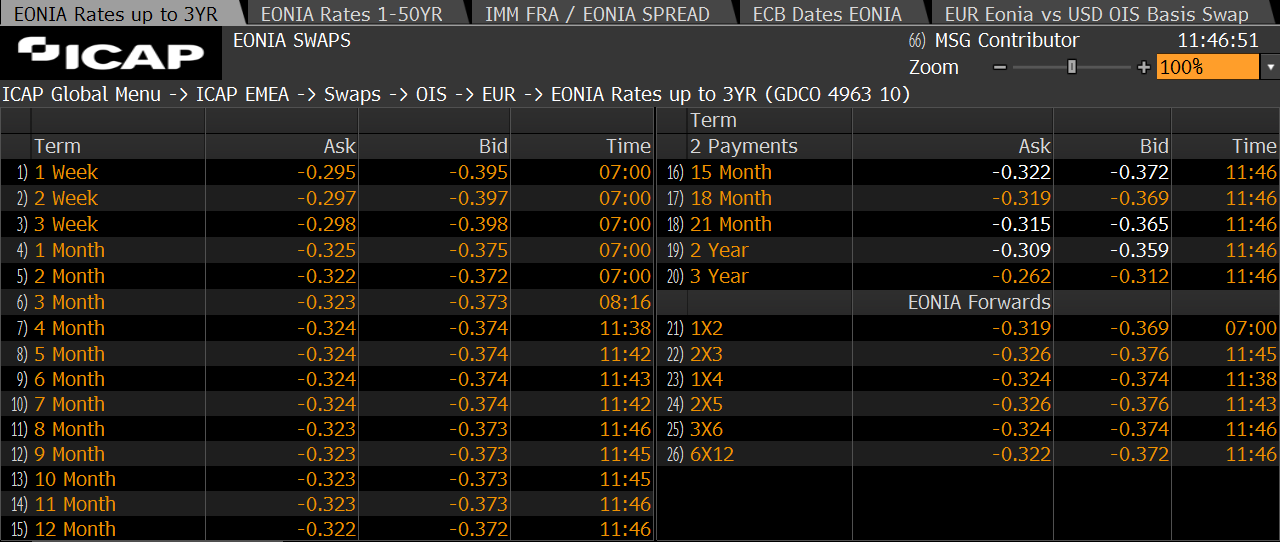
\includegraphics[width=1.\linewidth]{figures/icap_3.png}
\caption{Screenshot of market quotes from ICAP.}
\label{fig:icap}
\end{figure}

Though there exist some electronic platform in which market participants post bids and offers and other participants can apply them, in practice a lot of trading is still done over "voice", i.e.~by phone or more
commonly over chat. For convenience, however, Bloomberg provides a service which displays indicative real time rates as provided by a selection of relevant brokers. (\emph{N.B.~interest rate swap quotes vary from standard price quotes of commonly traded instruments, they can appear puzzling because the quotes are effectively interest rates})

In the following we use a similarly created data-set (\href{https://drive.google.com/file/d/1LCEDmheKqwPXFpJ25hFz32QI5im2UJO1/view?usp=sharing}{\texttt{ois\_data.xlsx}}) to derive our discount curve; with the help of the \texttt{pandas} module the data-set can be inspected:

\begin{tcolorbox}[breakable, size=fbox, boxrule=1pt, pad at break*=1mm,colback=cellbackground, colframe=cellborder]
\begin{Verbatim}[commandchars=\\\{\}]
\PY{k+kn}{import} \PY{n+nn}{pandas}\PY{o}{,} \PY{n+nn}{datetime}

\PY{n}{observation\PYZus{}date} \PY{o}{=} \PY{n}{datetime}\PY{o}{.}\PY{n}{date}\PY{o}{.}\PY{n}{today}\PY{p}{(}\PY{p}{)}

\PY{n}{mq} \PY{o}{=} \PY{n}{pandas}\PY{o}{.}\PY{n}{read\PYZus{}excel}\PY{p}{(}\PY{l+s+s1}{\PYZsq{}}\PY{l+s+s1}{ois\PYZus{}data.xlsx}\PY{l+s+s1}{\PYZsq{}}\PY{p}{)}
\PY{n}{mq}\PY{o}{.}\PY{n}{head}\PY{p}{(}\PY{p}{)}

   months  quote
0       1 -0.350
1       2 -0.347
2       3 -0.348
3       4 -0.350
4       5 -0.350
\end{Verbatim}
\end{tcolorbox}

Next we could convert the data-set into a dictionary for later usage or
use the \(\tt{DataFrame}\) directly, it is just matter of taste.

Let's say we want to build a 15 months swap instance using data
contained in \(\tt{ois\_data}\) file. Be careful when doing this
operation and double check the units of rates, quotes, etc\ldots{}in
this case for example quotes are expressed in percent so you need to
multiply them by 0.01 before using them. Another detail to check is that
15 months quote is not the fifteenth entry in the \(\tt{DataFrame}\)
(actually it is the twelfth).

\begin{tcolorbox}[breakable, size=fbox, boxrule=1pt, pad at break*=1mm, colback=cellbackground, colframe=cellborder]
\begin{Verbatim}[commandchars=\\\{\}]
\PY{n}{ois} \PY{o}{=} \PY{n}{OvernightIndexSwap}\PY{p}{(}\PY{l+m+mf}{1e6}\PY{p}{,}
                         \PY{p}{[}\PY{n}{date}\PY{p}{(}\PY{l+m+mi}{2019}\PY{p}{,} \PY{l+m+mi}{10}\PY{p}{,} \PY{l+m+mi}{23}\PY{p}{)}\PY{p}{,}
                          \PY{n}{date}\PY{p}{(}\PY{l+m+mi}{2020}\PY{p}{,} \PY{l+m+mi}{10}\PY{p}{,} \PY{l+m+mi}{23}\PY{p}{)}\PY{p}{,}
                          \PY{n}{date}\PY{p}{(}\PY{l+m+mi}{2020}\PY{p}{,} \PY{l+m+mi}{1}\PY{p}{,} \PY{l+m+mi}{23}\PY{p}{)}\PY{p}{]}\PY{p}{,}
                         \PY{n}{mq}\PY{p}{[}\PY{l+s+s1}{\PYZsq{}}\PY{l+s+s1}{quote}\PY{l+s+s1}{\PYZsq{}}\PY{p}{]}\PY{o}{.}\PY{n}{tolist}\PY{p}{(}\PY{p}{)}\PY{p}{[}\PY{l+m+mi}{12}\PY{p}{]}\PY{o}{*}\PY{l+m+mf}{0.01}\PY{p}{)}

\PY{c+c1}{\PYZsh{} print the last payment date }
\PY{c+c1}{\PYZsh{} (15 months after obs date)}
\PY{n}{ois}\PY{o}{.}\PY{n}{payment\PYZus{}dates}\PY{p}{[}\PY{o}{\PYZhy{}}\PY{l+m+mi}{1}\PY{p}{]}

datetime.date(2020, 1, 23)
\end{Verbatim}
\end{tcolorbox}

Clearly to use the \texttt{npv} method to calculate the OIS' NPV we need a discount curve with which to evaluate it and here comes to hand the bootstrapping technique !

\subsection{Constructing the Yield Curve}\label{the-bootstrapping-technique}

Keep aside for a moment our swaps and introduce the \emph{bootstrap
algorithm}. In finance, bootstrap is a method for constructing a
(zero-coupon) fixed-income yield curve from the prices of a set of
coupon-bearing products, e.g.~bonds and swaps. The term structure of
spot returns is obtained from the bond yields by solving for them
recursively, by forward substitution: this iterative process is what is
called the bootstrap method. The usefulness of bootstrap is that using
only a few carefully selected zero-coupon products, it becomes possible
to derive swap forward and spot rates for all maturities given the
solved curve.

To illustrate bootstrapping let's consider the following example which can be partially solved analytically: we have some coupon paying bond (coupon of 4\%, 5\%, 6\%, 7\% and 8\% respectively) with maturities ranging from 1 to 5 years, each having a value of \euro{100} and traded at par. To determine the zero-coupon yield curve proceed as follows:

\begin{enumerate}
\item at the end of the first year the $1^{st}$ bond will pay a coupon of \euro{4} (= \euro{100} * 4\%) plus the principal amount (= \euro{100}) which sums up to \euro{104} while the bond is trading at \euro{100}. Therefore, the implied 1-year spot \emph{fair} rate $S_{1y}$ can be calculated as, $\mbox{\euro{100}} = \mbox{\euro{104}} / (1 + S_{1y})$;

\item at the end of second year the sum of the cash flows of the $2^{nd}$ bond can be compared to its trading price to compute the 2-year spot rate $S_{2y}$ as $\mbox{\euro{100}} = \mbox{\euro{5}} / (1 + S_{1y}) + \mbox{\euro{105}} / (1 + S_{2y})^{2}$, using the previously derived value of $S_{1y}$;

\item at the end of third year the sum of the cash flows of the $3^{rd}$ bond can be compared to its trading price to calculate the 3-year spot rate $S_{3y}$ as $\mbox{\euro{100}} = \mbox{\euro{6}} / (1 + S_{1y}) + \mbox{\euro{6}} / (1 + S_{2y})^{2} + \mbox{\euro{106}} / (1 + S_{3y})^{3}$, using $S_{1y}$ and $S_{2y}$ computed before;

\item repeat the same reasoning for the other bonds.
\end{enumerate}

Putting all together we can construct a system of equations (now omitting the currency symbol for simplicity):

\begin{equation}
\begin{cases}
100 = \cfrac{104}{(1 + S_{1y})} \\
100 = \cfrac{5}{(1 + S_{1y})} + \cfrac{105}{(1 + S_{2y})^{2}} \\
100 = \cfrac{6} {(1 + S_{1y})} + \cfrac{6}{(1 + S_{2y})^{2}} + \cfrac{106} {(1 + S_{3y})^{3}} \\
100 = \cfrac{7} {(1 + S_{1y})} + \cfrac{7} {(1 + S_{2y})^{2}} + \cfrac{7} {(1 + S_{3y})^{3}} + \cfrac{107} {(1 + S_{4y})^{4}} \\
100 = \cfrac{8} {(1 + S_{1y})} + \cfrac{8} {(1 + S_{2y})^{2}}+ \cfrac{8} {(1 + S_{3y})^{3}} + \cfrac{8} {(1 + S_{4y})^{4}} + \cfrac{108} {(1 + S_{5y})^{5}}
\end{cases}
\label{eq:fifth_year_rate}
\end{equation}

This system can be solved quite easily: from the first equation can be derived $S_{1y}$, from the second $S_{2y}$, from the third $S_{3y}$ and so on. So

\[100 = 104 / (1 + S_{1y})\quad\Rightarrow\quad S_{1y} = 104/100 - 1 = 4\% \]

Moving to the second equation:

\begin{equation*}
\begin{split}
& 100 = 5 / (1 + 0.04) + 105 / (1 + S_{2y})^{2}\quad\Rightarrow\quad S_{2y}^2  + 2 S_{2y}  - 0.103030 = 0 \\
& S_{2y} = - 1 \pm \sqrt{1 + 0.103030} = \begin{cases}\text{\sout{-2.05023}} \\ 0.0503\end{cases}
\end{split}
\end{equation*}
where the first solution has been discarded because negative.

From the third one on it is not as simple to solve them analytically since involve third order (or more) equations, anyway it is possible to solve them numerically.
Assume we have found all the rates up to the fourth year (they are reported in Table~\ref{tab:rates}) and let's try to determine the last one.

\begin{table}[htb]
\begin{center}
\begin{tabular}{|c|c|c|c|}
\hline
\textbf{years} & \textbf{coupon rate} & \textbf{bond price} & \textbf{spot rate} \\
\hline
1 & 1.00 \% & \euro{100} & 4.00\% \\
\hline
2 & 2.00 \% & \euro{100} & 5.03\% \\
\hline
3 & 3.00 \% & \euro{100} & 6.08\% \\
\hline
4 & 4.00 \% & \euro{100} & 7.19\% \\
\hline
5 & 5.00 \% & \euro{100} & ??? \\
\hline
\end{tabular}
\end{center}
\caption{Table reporting maturity, coupon, bond price and implied spot rate for the example outlined in the text.}
\label{tab:rates}
\end{table}
The last column of Table~\ref{tab:rates} provides with the terms to fill the zero-coupon yield curve.
To solve the last equation numerically we can use the \texttt{scipy.optimize.brentq} function which finds the zeros of a user-defined function given a validity interval.
In Figure~\ref{fig:fifth_year_rate} the function to determine the 5 year rate expressed in the last of Eqs.~\ref{eq:fifth_year_rate} is shown. From the plot we expect tha rate to be around 8\%.

\begin{figure}[htb]
  \centering
  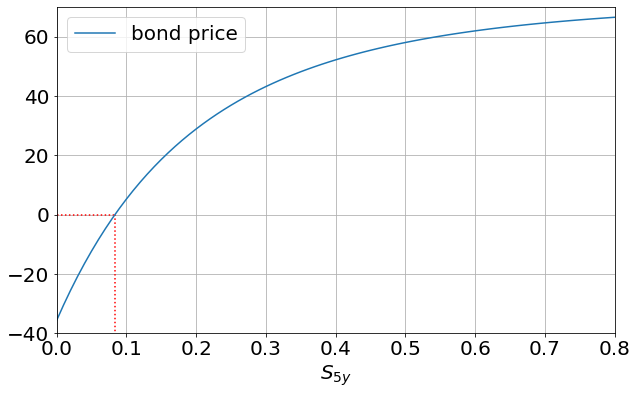
\includegraphics[width=0.7\textwidth]{figures/bond_5_plot.png}
  \caption{Plot of the discounted cash flow of bond 5 as a function of the 5 year spot rate.}
  \label{fig:fifth_year_rate}
\end{figure}

\begin{tcolorbox}[breakable, size=fbox, boxrule=1pt, pad at break*=1mm,colback=cellbackground, colframe=cellborder]
\begin{Verbatim}[commandchars=\\\{\}]
\PY{k+kn}{from} \PY{n+nn}{scipy}\PY{n+nn}{.}\PY{n+nn}{optimize} \PY{k}{import} \PY{n}{brentq}

\PY{k}{def} \PY{n+nf}{func}\PY{p}{(}\PY{n}{x}\PY{p}{)}\PY{p}{:}
    \PY{k}{return} \PY{l+m+mi}{100} \PY{o}{\PYZhy{}} \PY{l+m+mi}{8}\PY{o}{/}\PY{p}{(}\PY{l+m+mi}{1}\PY{o}{+}\PY{l+m+mf}{0.04}\PY{p}{)} \PY{o}{\PYZhy{}} \PY{l+m+mi}{8}\PY{o}{/}\PY{p}{(}\PY{l+m+mi}{1}\PY{o}{+}\PY{l+m+mf}{0.0503}\PY{p}{)}\PY{o}{*}\PY{o}{*}\PY{l+m+mi}{2} \PY{o}{\PYZhy{}} \PY{l+m+mi}{8}\PY{o}{/}\PY{p}{(}\PY{l+m+mi}{1}\PY{o}{+}\PY{l+m+mf}{0.0608}\PY{p}{)}\PY{o}{*}\PY{o}{*}\PY{l+m+mi}{3} 
               \PY{o}{\PYZhy{}} \PY{l+m+mi}{8}\PY{o}{/}\PY{p}{(}\PY{l+m+mi}{1}\PY{o}{+}\PY{l+m+mf}{0.0719}\PY{p}{)}\PY{o}{*}\PY{o}{*}\PY{l+m+mi}{4} \PY{o}{\PYZhy{}} \PY{l+m+mi}{108}\PY{o}{/}\PY{p}{(}\PY{l+m+mi}{1}\PY{o}{+}\PY{n}{x}\PY{p}{)}\PY{o}{*}\PY{o}{*}\PY{l+m+mi}{5}

\PY{n}{a} \PY{o}{=} \PY{n}{brentq}\PY{p}{(}\PY{n}{func}\PY{p}{,} \PY{l+m+mi}{0}\PY{p}{,} \PY{l+m+mf}{0.10}\PY{p}{)}
\PY{n+nb}{print} \PY{p}{(}\PY{l+s+s2}{\PYZdq{}}\PY{l+s+s2}{5y rate: }\PY{l+s+si}{\PYZob{}:.4f\PYZcb{}}\PY{l+s+s2}{\PYZdq{}}\PY{o}{.}\PY{n}{format}\PY{p}{(}\PY{n}{a}\PY{p}{)}\PY{p}{)}

5y rate: 0.0836
\end{Verbatim}
\end{tcolorbox}

The very same mechanism can be generalized and extended to more maturities to get a more detailed yield curve. In general terms the previous system can be written as:

\begin{equation*}
\begin{cases}
f_1(S_1, p_1) = 0 \\
f_2(S_1, S_2, p_2) = 0 \\
f_3(S_1, S_2, S_3, p_3) = 0 \\
f_4(S_1, S_2, S_3, S_4, p_4) = 0 \\
\cdots
\end{cases}
\end{equation*}
where $S_i$ are the unknown spot rates and $p_i$ the prices of the considered products. The iterative procedure we have applied before exploits the first equation to find $S_1 = f_1^{-1}(p_1)$, the second to find $S_2 = f_2^{-1}(S_1, p_2)$ and so on and so forth; this algorithm works since each equation will determine exactly one \emph{free} spot rate which is not already determined by the others.

\subsection{Bootstrap as Minimization Problem}
We can now describe the bootstrapping algorithm in general terms as follows:
\begin{enumerate}
\item define a set of yielding products , these will generally be coupon-bearing bonds;
\item derive discount factors for the corresponding terms;
\item \emph{bootstrap} the zero-coupon curve, successively calibrating the curve such that it returns the prices of these inputs.
\end{enumerate}

Instead of iteratively finding the solution of each equation as before, we could define a vector of spot rates $\mathbf{S} = (S_1, S_2, S_3, \ldots)$ seeking for a particular $\mathbf{\hat{S}}$ which solves the following equation:

\begin{equation*}
F = f_1^2(\hat{S}_1) + f_2^2(\hat{S}_1, \hat{S}_2) + f_3^2(\hat{S}_1, \hat{S}_2, \hat{S}_3) + f_4^2(\hat{S}_1, \hat{S}_2, \hat{S}_3, \hat{S}_4) + \ldots = 0
\end{equation*}

Under this terms bootstrapping can be considered as a minimization algorithm, indeed we need to find $\mathbf{\hat{S}}$ which \emph{minimize} $F$, or makes it as close as possible to 0.
Notice how each \(f_i\) is squared since we want all of them to be minimized and
not only \(F\) globally (without the squared there may be cancellation
effects between the terms of the sum).

\subsection{Minimization Algorithm}\label{minimization-algorithm}

A minimization algorithm follows these steps:

\begin{itemize}
\tightlist
\item
  define an \emph{objective function} i.e.~the function that is actually
  minimized to reach our goal;
\item
  set the initial value of the unknown parameters and their range of
  variability;
\item
  the minimizer will compute the objective function value;
\item
  then it will move the parameter values in such a way to find a smaller
  value of the objective function (e.g.~following the derivative w.r.t.
  each parameter);
\item if constraints are defined, they will be considered in the previous step;
\item
  the last three steps will be repeated until further variations of the
  \(\mathbf{x}\) values won't change significantly the objective
  function (i.e.~we have found a minimum of the function so the
  minimization process is completed !).
\end{itemize}

Let's see with a couple of example how minimization can be implemented in \texttt{python} using the function \texttt{scipy.optimize.minimize}.

\subsubsection{Example}\label{example}

Find the dimensions that will minimize the cost to
manufacture a circular cylindrical can of volume, \(330~\mathrm{cm}^3\), see Figure~\ref{fig:cylinder}.

\begin{figure}[h]
\centering
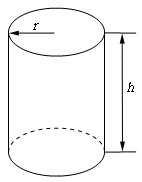
\includegraphics[width=0.2\textwidth]{figures/cylinder.png}
\caption{Graphical representation of the \emph{can} minimization example.}
\label{fig:cylinder}
\end{figure}

Clearly to minimize the costs the company needs to reduce the can
surface, given the required volume.

\[ S = 2\pi rh + 2\cdot(\pi r^2) \]

On the other hand we want the volume to be \(330~\mathrm{cm}^3\) so we
can remove \(h\) from the previous equation:

\[ V = \pi r^2 h = 330\quad\implies h = \cfrac{330}{\pi r^2} \]

So in the end the surface function to be minimized is:

\[ S = 2\pi rh + 2\cdot(\pi r^2) = \cfrac{2\cdot 330}{r} + 2\cdot(\pi r^2)\]

So we implement the objective function, \(\tt{x[0]}\) is the can radius:

\begin{tcolorbox}[breakable, size=fbox, boxrule=1pt, pad at break*=1mm,colback=cellbackground, colframe=cellborder]
\begin{Verbatim}[commandchars=\\\{\}]
\PY{k+kn}{from} \PY{n+nn}{math} \PY{k}{import} \PY{n}{pi}

\PY{k}{def} \PY{n+nf}{of}\PY{p}{(}\PY{n}{x}\PY{p}{)}\PY{p}{:}
    \PY{k}{return} \PY{l+m+mi}{2}\PY{o}{*}\PY{l+m+mi}{330}\PY{o}{/}\PY{n}{x}\PY{p}{[}\PY{l+m+mi}{0}\PY{p}{]} \PY{o}{+} \PY{l+m+mi}{2}\PY{o}{*}\PY{n}{pi}\PY{o}{*}\PY{n}{x}\PY{p}{[}\PY{l+m+mi}{0}\PY{p}{]}\PY{o}{*}\PY{o}{*}\PY{l+m+mi}{2}
\end{Verbatim}
\end{tcolorbox}

Set the limits to our unknown variable and its initial value:

\begin{tcolorbox}[breakable, size=fbox, boxrule=1pt, pad at break*=1mm,colback=cellbackground, colframe=cellborder]
\begin{Verbatim}[commandchars=\\\{\}]
\PY{n}{x0} \PY{o}{=} \PY{p}{[}\PY{l+m+mi}{1}\PY{p}{]}
\PY{n}{bounds} \PY{o}{=} \PY{p}{[}\PY{p}{(}\PY{l+m+mf}{0.01}\PY{p}{,} \PY{l+m+mi}{100}\PY{p}{)}\PY{p}{]}
\end{Verbatim}
\end{tcolorbox}

    Finally we run the minimization:

    \begin{tcolorbox}[breakable, size=fbox, boxrule=1pt, pad at break*=1mm,colback=cellbackground, colframe=cellborder]
\begin{Verbatim}[commandchars=\\\{\}]
\PY{n}{r} \PY{o}{=} \PY{n}{minimize}\PY{p}{(}\PY{n}{of}\PY{p}{,} \PY{n}{x0}\PY{p}{,} \PY{n}{bounds}\PY{o}{=}\PY{n}{bounds}\PY{p}{)}
\PY{n+nb}{print} \PY{p}{(}\PY{n}{r}\PY{p}{)}

      fun: 264.356810914805
 hess\_inv: <1x1 LbfgsInvHessProduct with dtype=float64>
      jac: array([5.68434189e-06])
  message: b'CONVERGENCE: NORM\_OF\_PROJECTED\_GRADIENT\_<=\_PGTOL'
     nfev: 24
      nit: 9
   status: 0
  success: True
        x: array([3.7449385])
    \end{Verbatim}
\end{tcolorbox}

    So to minimize the cost the company should produce cans with a radius of
about 3.745 cm (I suspect that Coke have done a similar calculation...).

\subsubsection{Example with Constraint}\label{example-with-constraint}

We are going to fence in a rectangular field. If we look at the field
from above the cost of the vertical sides are \$10/m, the cost of the
bottom is \$2/m and the cost of the top is \$7/m. If we have \$700 determine
the dimensions of the field that will maximize the enclosed area, see Fig.~\ref{fig:field}.

\begin{figure}[h]
\centering
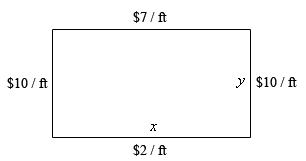
\includegraphics[width=0.4\textwidth]{figures/field.png}
\caption{Graphical representation of the \emph{field} minimization example.}
\label{fig:field}
\end{figure}

In this example there are two differences with respect to the previous one:

\begin{itemize}
\tightlist
\item
  we want to maximize a quantity (not minimize);
\item
  there is a constraint (we have a limited amount of money).
\end{itemize}

So let's repeat the steps as before. The objective is to maximize the
enclosed area \(A\) but we are able to just minimize so we can define in the objective function the quantity \(-A\), if we minimize it
we will maximize the area $A$. Define the length and the width of the field with \(\tt{x[0]}\) and
\(\tt{x[1]}\) (items of the list \(\tt{x}\):

    \begin{tcolorbox}[breakable, size=fbox, boxrule=1pt, pad at break*=1mm,colback=cellbackground, colframe=cellborder]
\begin{Verbatim}[commandchars=\\\{\}]
\PY{k}{def} \PY{n+nf}{of}\PY{p}{(}\PY{n}{x}\PY{p}{)}\PY{p}{:}
    \PY{k}{return} \PY{o}{\PYZhy{}} \PY{n}{x}\PY{p}{[}\PY{l+m+mi}{0}\PY{p}{]}\PY{o}{*}\PY{n}{x}\PY{p}{[}\PY{l+m+mi}{1}\PY{p}{]}
\end{Verbatim}
\end{tcolorbox}

    Now we can set the boundaries for length and width and their initial
values (1 m each):

    \begin{tcolorbox}[breakable, size=fbox, boxrule=1pt, pad at break*=1mm,colback=cellbackground, colframe=cellborder]
\begin{Verbatim}[commandchars=\\\{\}]
\PY{n}{x0} \PY{o}{=} \PY{p}{[}\PY{l+m+mi}{1}\PY{p}{,} \PY{l+m+mi}{1}\PY{p}{]}
\PY{n}{bounds} \PY{o}{=} \PY{p}{[}\PY{p}{(}\PY{l+m+mf}{0.01}\PY{p}{,} \PY{l+m+mi}{100}\PY{p}{)} \PY{k}{for} \PY{n}{\PYZus{}} \PY{o+ow}{in} \PY{n+nb}{range}\PY{p}{(}\PY{n+nb}{len}\PY{p}{(}\PY{n}{x0}\PY{p}{)}\PY{p}{)}\PY{p}{]}
\end{Verbatim}
\end{tcolorbox}

    We have also to impose the constraint on the money. This is done by
defining a function that compute the money spent with the fence and
compare it to \$700. The constraint is passed to the minimizer with a
dictionary which has two keys: \(\tt{type}\) with value \(\tt{eq}\)
(like equality) since we want to spend all of our available money so the
fence has to cost \$700

\[\mathrm{fence~cost} = l\cdot10 + l\cdot10 + w\cdot2 + w\cdot7 = 700\]
\[700 - l\cdot10 - l\cdot10 - w\cdot2 - w\cdot7 = 0\],
\(\tt{fun}\) whose value is the constraint function.

\begin{tcolorbox}[breakable, size=fbox, boxrule=1pt, pad at break*=1mm,colback=cellbackground, colframe=cellborder]
\begin{Verbatim}[commandchars=\\\{\}]
\PY{k}{def} \PY{n+nf}{cons}\PY{p}{(}\PY{n}{x}\PY{p}{)}\PY{p}{:}
    \PY{k}{return} \PY{l+m+mi}{700} \PY{o}{\PYZhy{}} \PY{n}{x}\PY{p}{[}\PY{l+m+mi}{0}\PY{p}{]}\PY{o}{*}\PY{l+m+mi}{20} \PY{o}{\PYZhy{}} \PY{n}{x}\PY{p}{[}\PY{l+m+mi}{1}\PY{p}{]}\PY{o}{*}\PY{l+m+mi}{2} \PY{o}{\PYZhy{}} \PY{n}{x}\PY{p}{[}\PY{l+m+mi}{1}\PY{p}{]}\PY{o}{*}\PY{l+m+mi}{7}

\PY{n}{constraints} \PY{o}{=} \PY{p}{\PYZob{}}\PY{l+s+s1}{\PYZsq{}}\PY{l+s+s1}{type}\PY{l+s+s1}{\PYZsq{}}\PY{p}{:}\PY{l+s+s1}{\PYZsq{}}\PY{l+s+s1}{eq}\PY{l+s+s1}{\PYZsq{}}\PY{p}{,} \PY{l+s+s1}{\PYZsq{}}\PY{l+s+s1}{fun}\PY{l+s+s1}{\PYZsq{}}\PY{p}{:}\PY{n}{cons}\PY{p}{\PYZcb{}}
\end{Verbatim}
\end{tcolorbox}

    Now we can call the minimizer.

    \begin{tcolorbox}[breakable, size=fbox, boxrule=1pt, pad at break*=1mm,colback=cellbackground, colframe=cellborder]
\begin{Verbatim}[commandchars=\\\{\}]
\PY{n}{r} \PY{o}{=} \PY{n}{minimize}\PY{p}{(}\PY{n}{of}\PY{p}{,} \PY{n}{x0}\PY{p}{,} \PY{n}{bounds}\PY{o}{=}\PY{n}{bounds}\PY{p}{,} \PY{n}{constraints}\PY{o}{=}\PY{n}{constraints}\PY{p}{)}
\PY{n+nb}{print} \PY{p}{(}\PY{n}{r}\PY{p}{)}

     fun: -680.5555555555482
     jac: array([-38.88889313, -17.5       ])
 message: 'Optimization terminated successfully.'
    nfev: 16
     nit: 4
    njev: 4
  status: 0
 success: True
       x: array([17.49999818, 38.88889293])
    \end{Verbatim}
\end{tcolorbox}

So the field will come out \(17.5\)m long and \(38.9\)m wide.

\subsection{Local Minima}
When the objective function has local minima the choice of the initial value of the parameters can be critical. 
Assume we would like to minimize an objective function like 

\[
f(x) = \cfrac{\mathrm{cos}(3\pi x)}{x}
\]
This function is plotted in Fig.~\ref{fig:local_minima} in the range $[0, 2]$, and it is clear that it has many minima. 

\begin{figure}[htb]
	\centering
	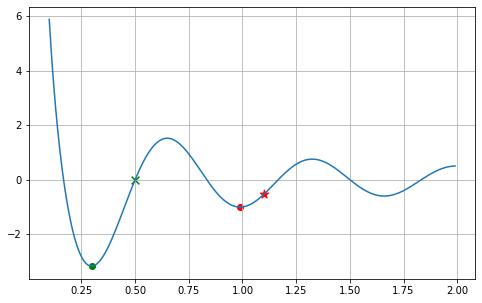
\includegraphics[width=0.7\textwidth]{figures/lesson4_39_0.png}
\caption{Plot of an example function with many local minima. The red points highlights initial value and minimum found in a \emph{bad} minimization, green points for a good minimization.}
\label{fig:local_minima}
\end{figure}

Let's try to find a minimum and set the initial value to $x=1.1$.
\begin{tcolorbox}[breakable, size=fbox, boxrule=1pt, pad at break*=1mm,colback=cellbackground, colframe=cellborder]
\begin{Verbatim}[commandchars=\\\{\}]
\PY{k+kn}{from} \PY{n+nn}{scipy}\PY{n+nn}{.}\PY{n+nn}{optimize} \PY{k}{import} \PY{n}{minimize}
\PY{n}{x0} \PY{o}{=} \PY{p}{[}\PY{l+m+mf}{1.1}\PY{p}{]}
\PY{n}{bounds} \PY{o}{=} \PY{p}{[}\PY{p}{(}\PY{l+m+mf}{0.01}\PY{p}{,} \PY{l+m+mi}{20}\PY{p}{)}\PY{p}{]}
		
\PY{n}{r} \PY{o}{=} \PY{n}{minimize}\PY{p}{(}\PY{n}{func}\PY{p}{,} \PY{n}{x0}\PY{p}{,} \PY{n}{bounds}\PY{o}{=}\PY{n}{bounds}\PY{p}{)}
\PY{n}{r}

fun: array([-1.00569871])
hess\_inv: <1x1 LbfgsInvHessProduct with dtype=float64>
jac: array([-4.4408921e-07])
message: b'CONVERGENCE: NORM\_OF\_PROJECTED\_GRADIENT\_<=\_PGTOL'
nfev: 16
nit: 5
status: 0
success: True
x: array([0.98865633])
\end{Verbatim}
\end{tcolorbox}
The minimization worked perfectly and we found $x=0.98865633$ (i.e. the red point in Fig.~\ref{fig:local_minima}) but still from the same Figure it is clear that this is not the absolute minimum we would like to find. The problem arise since the algorithm has got stuck in this local minimum without any possibility to jump out from the well.

If we repeat the minimization using as initial value $0.5$ instead
\begin{tcolorbox}[breakable, size=fbox, boxrule=1pt, pad at break*=1mm,colback=cellbackground, colframe=cellborder]
\begin{Verbatim}[commandchars=\\\{\}]
\PY{k+kn}{from} \PY{n+nn}{scipy}\PY{n+nn}{.}\PY{n+nn}{optimize} \PY{k}{import} \PY{n}{minimize}
\PY{n}{x0} \PY{o}{=} \PY{p}{[}\PY{l+m+mf}{0.5}\PY{p}{]}
\PY{n}{bounds} \PY{o}{=} \PY{p}{[}\PY{p}{(}\PY{l+m+mf}{0.01}\PY{p}{,} \PY{l+m+mi}{20}\PY{p}{)}\PY{p}{]}
		
\PY{n}{r} \PY{o}{=} \PY{n}{minimize}\PY{p}{(}\PY{n}{func}\PY{p}{,} \PY{n}{x0}\PY{p}{,} \PY{n}{bounds}\PY{o}{=}\PY{n}{bounds}\PY{p}{)}
\PY{n}{r}

fun: array([-3.17151711])
hess\_inv: <1x1 LbfgsInvHessProduct with dtype=float64>
jac: array([9.76996262e-07])
message: b'CONVERGENCE: NORM\_OF\_PROJECTED\_GRADIENT\_<=\_PGTOL'
nfev: 16
nit: 5
status: 0
success: True
x: array([0.29691798])
\end{Verbatim}
\end{tcolorbox}
Now clearly the algorithm found the absolute minimum in $x=0.29691798$ (i.e. the green point in Fig.~\ref{fig:local_minima}) because there was no chance to find a local minimum during the iterations.

This is clearly an example of what could happen, the possible solution is to make a \emph{scan} of the objective function to try to approximately determine where the global minimum is and choose the \emph{right} initial values for our parameters.
There should be such an issue in the application of the bootstrapping algorithm though since the function that we are going to minimize is a sum of squared terms which has no local minima, just a global minimum (i.e. it is a parabola).


\subsection{OIS Example}\label{ois-example}
Back to our Overnight Index Swap, the general idea here is to get the discount curve \(\mathcal{C}\) such that it prices correctly each OIS by minimizing the sum of their NPV squared (our \(f_i\)):

\[\mathrm{min}_{\mathcal{C}} \Big\{\sum_{i=1}^{n}\mathrm{NPV}(\mathrm{OIS}_i, \mathcal{C})^2\Big\}\]

A discount curve is characterized by pillar dates and the corresponding discount factors. The description of the problem we have given above does not, in theory, specifies any constraint on the number of pillar dates of the discount curve \(\mathcal{C}\). However, the pillar dates determine the number of unknown variables (i.e.~the dimensionality \(N\) of the optimization problem). A curve with \(N\) pillar dates has \(N\) discount factors (note that the first discount factor with value date equal to the today date, is constrained to 1). \textbf{In practice, therefore, it makes sense to choose the pillar dates in such a way that there are exactly the right number of degrees of freedom in the optimization to match data.} So the natural choice is to choose the pillar dates of the discount curve equal to the set of expiry dates of the swaps.

Once we've fixed \(\mathbf{d}\) to be a vector of pillar dates equal to the expiry dates of the swaps, and we use the notation \(\mathbf{x}\) to represent the vector of pillar discount factors, then the problem becomes:

\[\mathrm{min}_{\mathbf{x}} \Big\{\sum_{i=1}^{N}\mathrm{NPV}(\mathrm{OIS}_i, \mathcal{C}(\mathbf{d}, \mathbf{x}))^2\Big\}\]
which is our optimization problem (\textbf{to find the minimum of the
above expression as a function of x}) that can be solved using one of
the available numerical optimization routines in \(\tt{python}\).

So first let's create the swaps according to all the available market
quotes and also the pillar dates of our final discount curve:

    \begin{tcolorbox}[breakable, size=fbox, boxrule=1pt, pad at break*=1mm,colback=cellbackground, colframe=cellborder]
\begin{Verbatim}[commandchars=\\\{\}]
\PY{k+kn}{from} \PY{n+nn}{finmarkets} \PY{k}{import} \PY{n}{generate\PYZus{}swap\PYZus{}dates}

\PY{n}{observation\PYZus{}date} \PY{o}{=} \PY{n}{date}\PY{p}{(}\PY{l+m+mi}{2019}\PY{p}{,} \PY{l+m+mi}{10}\PY{p}{,} \PY{l+m+mi}{23}\PY{p}{)}
\PY{n}{pillar\PYZus{}dates} \PY{o}{=} \PY{p}{[}\PY{n}{observation\PYZus{}date}\PY{p}{]}
\PY{n}{swaps} \PY{o}{=} \PY{p}{[}\PY{p}{]} \PY{c+c1}{\PYZsh{} container of the OIS objects}

\PY{k}{for} \PY{n}{i} \PY{o+ow}{in} \PY{n+nb}{range}\PY{p}{(}\PY{n+nb}{len}\PY{p}{(}\PY{n}{df}\PY{p}{)}\PY{p}{)}\PY{p}{:}
    \PY{n}{swap} \PY{o}{=} \PY{n}{OvernightIndexSwap}\PY{p}{(}\PY{l+m+mf}{1e6}\PY{p}{,}
                    \PY{n}{generate\PYZus{}swap\PYZus{}dates}\PY{p}{(}
                        \PY{n}{observation\PYZus{}date}\PY{p}{,} 
                        \PY{n}{mq}\PY{p}{[}\PY{l+s+s1}{\PYZsq{}}\PY{l+s+s1}{months}\PY{l+s+s1}{\PYZsq{}}\PY{p}{]}\PY{o}{.}\PY{n}{tolist}\PY{p}{(}\PY{p}{)}\PY{p}{[}\PY{n}{i}\PY{p}{]}\PY{p}{)}\PY{p}{,}
                    \PY{l+m+mf}{0.01} \PY{o}{*} \PY{n}{mq}\PY{p}{[}\PY{l+s+s1}{\PYZsq{}}\PY{l+s+s1}{quote}\PY{l+s+s1}{\PYZsq{}}\PY{p}{]}\PY{o}{.}\PY{n}{tolist}\PY{p}{(}\PY{p}{)}\PY{p}{[}\PY{n}{i}\PY{p}{]}\PY{p}{)}

    \PY{n}{swaps}\PY{o}{.}\PY{n}{append}\PY{p}{(}\PY{n}{swap}\PY{p}{)}
    \PY{n}{pillar\PYZus{}dates}\PY{o}{.}\PY{n}{append}\PY{p}{(}\PY{n}{swap}\PY{o}{.}\PY{n}{payment\PYZus{}dates}\PY{p}{[}\PY{o}{\PYZhy{}}\PY{l+m+mi}{1}\PY{p}{]}\PY{p}{)}

\PY{c+c1}{\PYZsh{} this shouldn\PYZsq{}t be necessary if the original}
\PY{c+c1}{\PYZsh{} list of market quotes is sorted}
\PY{n}{pillar\PYZus{}dates} \PY{o}{=} \PY{n+nb}{sorted}\PY{p}{(}\PY{n}{pillar\PYZus{}dates}\PY{p}{)}
\end{Verbatim}
\end{tcolorbox}

So let's implement the method with the swaps we have just created, of course we don't need to write our minimisation algorithm since we can use the one provided by \texttt{python} which is defined in \texttt{scipy.optimize}, function \texttt{minimize}.

\begin{itemize}
\tightlist
\item
  define the objective function: the sum of the squared NPVs of the OIS

    \begin{tcolorbox}[breakable, size=fbox, boxrule=1pt, pad at break*=1mm,colback=cellbackground, colframe=cellborder]
\begin{Verbatim}[commandchars=\\\{\}]
\PY{k}{def} \PY{n+nf}{objective\PYZus{}function}\PY{p}{(}\PY{n}{x}\PY{p}{)}\PY{p}{:}
    \PY{n}{curve} \PY{o}{=} \PY{n}{DiscountCurve}\PY{p}{(}\PY{n}{observation\PYZus{}date}\PY{p}{,}
                          \PY{n}{pillar\PYZus{}dates}\PY{p}{,}
                          \PY{n}{x}\PY{p}{)}
    
    \PY{n}{sum\PYZus{}sq} \PY{o}{=} \PY{l+m+mf}{0.0}
    \PY{k}{for} \PY{n}{swap} \PY{o+ow}{in} \PY{n}{swaps}\PY{p}{:}
        \PY{n}{sum\PYZus{}sq} \PY{o}{+}\PY{o}{=} \PY{n}{swap}\PY{o}{.}\PY{n}{npv}\PY{p}{(}\PY{n}{curve}\PY{p}{)} \PY{o}{*}\PY{o}{*} \PY{l+m+mi}{2}
    \PY{k}{return} \PY{n}{sum\PYZus{}sq}
\end{Verbatim}
\end{tcolorbox}

\item
  set the initial value of the discount factors (\(x_i^0\)) to 1 with a
  range of variability \([ 0.01, 10]\), in addition the first element of
  the list, today's discount factor, will be fixed to 1 (variability
  \([1, 1]\))

    \begin{tcolorbox}[breakable, size=fbox, boxrule=1pt, pad at break*=1mm,colback=cellbackground, colframe=cellborder]
\begin{Verbatim}[commandchars=\\\{\}]
\PY{n}{x0} \PY{o}{=} \PY{p}{[}\PY{l+m+mf}{1.0} \PY{k}{for} \PY{n}{i} \PY{o+ow}{in} \PY{n+nb}{range}\PY{p}{(}\PY{n+nb}{len}\PY{p}{(}\PY{n}{pillar\PYZus{}dates}\PY{p}{)}\PY{p}{)}\PY{p}{]}

\PY{n}{bounds} \PY{o}{=} \PY{p}{[}\PY{p}{(}\PY{l+m+mf}{0.01}\PY{p}{,} \PY{l+m+mf}{10.0}\PY{p}{)} \PY{k}{for} \PY{n}{i} \PY{o+ow}{in} \PY{n+nb}{range}\PY{p}{(}\PY{n+nb}{len}\PY{p}{(}\PY{n}{pillar\PYZus{}dates}\PY{p}{)}\PY{p}{)}\PY{p}{]}
\PY{n}{bounds}\PY{p}{[}\PY{l+m+mi}{0}\PY{p}{]} \PY{o}{=} \PY{p}{(}\PY{l+m+mf}{1.0}\PY{p}{,} \PY{l+m+mf}{1.0}\PY{p}{)}
\end{Verbatim}
\end{tcolorbox}

\item
  finally we can launch the minimizer to find the discount factors
  (\(x\))

    \begin{tcolorbox}[breakable, size=fbox, boxrule=1pt, pad at break*=1mm,colback=cellbackground, colframe=cellborder]
\begin{Verbatim}[commandchars=\\\{\}]
\PY{k+kn}{from} \PY{n+nn}{scipy}\PY{n+nn}{.}\PY{n+nn}{optimize} \PY{k}{import} \PY{n}{minimize}

\PY{n}{result} \PY{o}{=} \PY{n}{minimize}\PY{p}{(}\PY{n}{objective\PYZus{}function}\PY{p}{,} \PY{n}{x0}\PY{p}{,} \PY{n}{bounds}\PY{o}{=}\PY{n}{bounds}\PY{p}{)}
\PY{n+nb}{print} \PY{p}{(}\PY{n}{result}\PY{p}{)}
\end{Verbatim}
\end{tcolorbox}

    \begin{Verbatim}[commandchars=\\\{\}]
      fun: 0.000819919032900304
 hess\_inv: <34x34 LbfgsInvHessProduct with dtype=float64>
      jac: array([ 6.58948735e+05, -1.58720803e+01, -6.53143264e+01,
-1.03323232e+02,
       -1.26050260e+02, -1.31748898e+02, -1.20374599e+02, -9.15399651e+01,
       -4.24363322e+01,  2.44903182e+01,  1.14345243e+02,  2.22002243e+02,
       -3.72021700e+00,  4.21398633e+01,  4.21787852e+01,  4.22369487e+01,
        4.23327026e+01,  4.31814758e+01,  4.44924460e+01,  4.62078978e+01,
        4.82906823e+01, -3.69972738e+00, -1.42454702e+00,  7.53771932e-01,
        2.79741018e+00,  4.62896699e+00,  6.24844054e+00,  9.93101553e+00,
        1.31122434e+01,  1.42880909e+01,  1.48279215e+01,  1.50787019e+01,
        1.43267935e+01,  1.38451324e+01])
  message: b'CONVERGENCE: REL\_REDUCTION\_OF\_F\_<=\_FACTR*EPSMCH'
     nfev: 840
      nit: 7
   status: 0
  success: True
        x: array([1.        , 1.00030147, 1.00058831, 1.00089012, 1.00119726,
       1.00147996, 1.00178743, 1.00208107, 1.00238467, 1.00267865,
       1.00298261, 1.00327737, 1.00357104, 1.00357104, 1.00355063,
       1.00352002, 1.00346901, 1.00302007, 1.00232627, 1.00141821,
       1.00031629, 0.99911234, 0.99790839, 0.99675545, 0.99567393,
       0.99470465, 0.9938476 , 0.99189884, 0.99021534, 0.98959296,
       0.98930728, 0.98917464, 0.98957256, 0.98982763])
    \end{Verbatim}
\end{itemize}

Printing the result gives us the a lot of information about the minimisation just performed, the most useful are:
\begin{itemize}
\item \texttt{func}: the value of the objective function at the last iteration;
\item \texttt{message}: the summary message from the algorithm (if it is \texttt{CONVERGENCE} is OK);
\item \texttt{success}: the name is self explanatory;
\item \texttt{x}: the vector of unknown parameters that have been optimised.
\end{itemize}

Another useful check to perform in order to understand if everything went fine, is the comparison of the objective function with the initial guessed parameters and at the end of the minimisation.

\begin{tcolorbox}[breakable, size=fbox, boxrule=1pt, pad at break*=1mm,colback=cellbackground, colframe=cellborder]
\begin{Verbatim}[commandchars=\\\{\}]
\PY{n+nb}{print} \PY{p}{(}\PY{l+s+s2}{\PYZdq{}}\PY{l+s+s2}{Initial objective function value }\PY{l+s+s2}{\PYZdq{}}\PY{p}{,} \PY{n}{objective\PYZus{}function}\PY{p}{(}\PY{n}{x0}\PY{p}{)}\PY{p}{)}
\PY{n+nb}{print} \PY{p}{(}\PY{l+s+s2}{\PYZdq{}}\PY{l+s+s2}{Final objective function value }\PY{l+s+s2}{\PYZdq{}}\PY{p}{,} \PY{n}{objective\PYZus{}function}\PY{p}{(}\PY{n}{result}\PY{o}{.}\PY{n}{x}\PY{p}{)}\PY{p}{)}

Initial objective function value  931188216.6666666
Final objective function value  0.000819919032900304
    \end{Verbatim}
\end{tcolorbox}
The objective function at the end of the minimisation is not exactly 0 (and rarely it will be) but its value is small enough for us to be satisfied, we started with $10^{10}$ and now it is $10^{-4}$ so 14 orders of magnitude smaller. This means that with the derived discount curve the NPV's of our OIS won't be identically 0 but so small that we can consider them as they were.

It can be very useful to also look at some diagnostic plots to check if the minimization was successful. Figure~\ref{fig:minimization_diagnostic} reports on the left the objective function value as a function of discount factor $(x_1)$; clearly we have found a minimum (the orange point represent $x_1$ value at the end of the minimization). On the right the value of the objective function at each iteration is shown instead, its value is decreasing dramatically (notice that the $y$ axis is drawn in log scale).

\begin{figure}[htb]
  \centering
  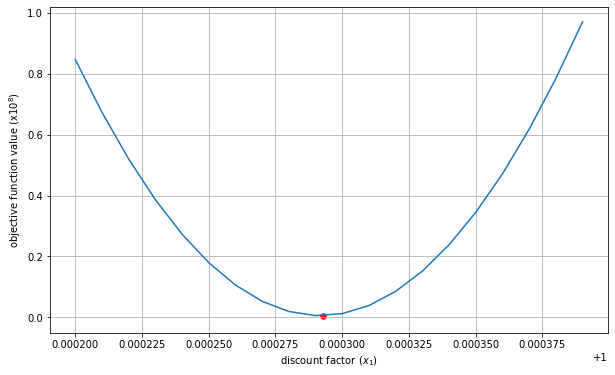
\includegraphics[width=0.45\linewidth]{figures/obj_func.png}
  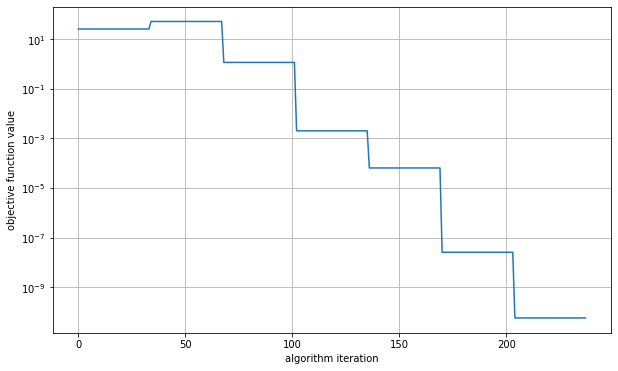
\includegraphics[width=0.45\linewidth]{figures/obj_func_iter.png}
  \caption{Diagnostic plots for the minimization algorithm. On the left the objective function value as a function of the discount factor $x_1$, on the right the objective function value as a function of the iteration number (the orange point represent $x_1$ value at the end of the minimization).}
  \label{fig:minimization_diagnostic}
\end{figure}

Finally we can create the discount curve implied by the market quote of
our swaps (see Fig.~\ref{fig:discount_curve}) and try to compute some implied rate.

\begin{tcolorbox}[breakable, size=fbox, boxrule=1pt, pad at break*=1mm,colback=cellbackground, colframe=cellborder]
\begin{Verbatim}[commandchars=\\\{\}]
\PY{k+kn}{from} \PY{n+nn}{math} \PY{k}{import} \PY{n}{log}
\PY{n}{curve} \PY{o}{=} \PY{n}{DiscountCurve}\PY{p}{(}\PY{n}{observation\PYZus{}date}\PY{p}{,} \PY{n}{pillar\PYZus{}dates}\PY{p}{,} \PY{n}{result}\PY{o}{.}\PY{n}{x}\PY{p}{)}

\PY{n}{d} \PY{o}{=} \PY{n}{date}\PY{p}{(}\PY{l+m+mi}{2059}\PY{p}{,} \PY{l+m+mi}{11}\PY{p}{,} \PY{l+m+mi}{23}\PY{p}{)}
\PY{n+nb}{print} \PY{p}{(}\PY{l+s+s2}{\PYZdq{}}\PY{l+s+s2}{40y df: }\PY{l+s+si}{\PYZob{}\PYZcb{}}\PY{l+s+s2}{\PYZdq{}}\PY{o}{.}\PY{n}{format}\PY{p}{(}\PY{n}{curve}\PY{o}{.}\PY{n}{df}\PY{p}{(}\PY{n}{d}\PY{p}{)}\PY{p}{)}\PY{p}{)}
\PY{n+nb}{print} \PY{p}{(}\PY{l+s+s2}{\PYZdq{}}\PY{l+s+s2}{40y rate: }\PY{l+s+si}{\PYZob{}\PYZcb{}}\PY{l+s+s2}{\PYZdq{}}\PY{o}{.}\PY{n}{format}\PY{p}{(}\PY{o}{\PYZhy{}}\PY{n}{log}\PY{p}{(}\PY{n}{curve}\PY{o}{.}\PY{n}{df}\PY{p}{(}\PY{n}{d}\PY{p}{)}\PY{p}{)} \PY{o}{/} \PY{l+m+mi}{40}\PY{p}{)}\PY{p}{)}             

40y df: 0.9891780176191146
40y rate: 0.0002720241491103593
    \end{Verbatim}
\end{tcolorbox}

\begin{figure}[htb]
  \centering
  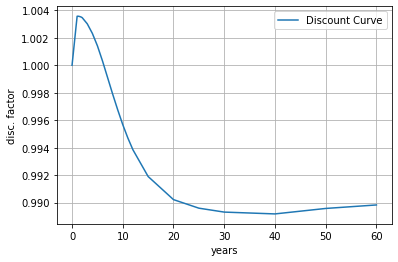
\includegraphics[width=0.7\textwidth]{figures/bootstrap_23_0.png}
  \caption{Plot of the discount curve implied by Overnight Index Swap market quotes.}
  \label{fig:discount_curve}
\end{figure}


%\clearpage
%\documentclass[11pt]{article}

    \usepackage[breakable]{tcolorbox}
    \usepackage{parskip} % Stop auto-indenting (to mimic markdown behaviour)
    
    \usepackage{iftex}
    \ifPDFTeX
    	\usepackage[T1]{fontenc}
    	\usepackage{mathpazo}
    \else
    	\usepackage{fontspec}
    \fi

    % Basic figure setup, for now with no caption control since it's done
    % automatically by Pandoc (which extracts ![](path) syntax from Markdown).
    \usepackage{graphicx}
    % Maintain compatibility with old templates. Remove in nbconvert 6.0
    \let\Oldincludegraphics\includegraphics
    % Ensure that by default, figures have no caption (until we provide a
    % proper Figure object with a Caption API and a way to capture that
    % in the conversion process - todo).
    \usepackage{caption}
    \DeclareCaptionFormat{nocaption}{}
    \captionsetup{format=nocaption,aboveskip=0pt,belowskip=0pt}

    \usepackage[Export]{adjustbox} % Used to constrain images to a maximum size
    \adjustboxset{max size={0.9\linewidth}{0.9\paperheight}}
    \usepackage{float}
    \floatplacement{figure}{H} % forces figures to be placed at the correct location
    \usepackage{xcolor} % Allow colors to be defined
    \usepackage{enumerate} % Needed for markdown enumerations to work
    \usepackage{geometry} % Used to adjust the document margins
    \usepackage{amsmath} % Equations
    \usepackage{amssymb} % Equations
    \usepackage{textcomp} % defines textquotesingle
    % Hack from http://tex.stackexchange.com/a/47451/13684:
    \AtBeginDocument{%
        \def\PYZsq{\textquotesingle}% Upright quotes in Pygmentized code
    }
    \usepackage{upquote} % Upright quotes for verbatim code
    \usepackage{eurosym} % defines \euro
    \usepackage[mathletters]{ucs} % Extended unicode (utf-8) support
    \usepackage{fancyvrb} % verbatim replacement that allows latex
    \usepackage{grffile} % extends the file name processing of package graphics 
                         % to support a larger range
    \makeatletter % fix for grffile with XeLaTeX
    \def\Gread@@xetex#1{%
      \IfFileExists{"\Gin@base".bb}%
      {\Gread@eps{\Gin@base.bb}}%
      {\Gread@@xetex@aux#1}%
    }
    \makeatother

    % The hyperref package gives us a pdf with properly built
    % internal navigation ('pdf bookmarks' for the table of contents,
    % internal cross-reference links, web links for URLs, etc.)
    \usepackage{hyperref}
    % The default LaTeX title has an obnoxious amount of whitespace. By default,
    % titling removes some of it. It also provides customization options.
    \usepackage{titling}
    \usepackage{longtable} % longtable support required by pandoc >1.10
    \usepackage{booktabs}  % table support for pandoc > 1.12.2
    \usepackage[inline]{enumitem} % IRkernel/repr support (it uses the enumerate* environment)
    \usepackage[normalem]{ulem} % ulem is needed to support strikethroughs (\sout)
                                % normalem makes italics be italics, not underlines
    \usepackage{mathrsfs}
    

    
    % Colors for the hyperref package
    \definecolor{urlcolor}{rgb}{0,.145,.698}
    \definecolor{linkcolor}{rgb}{.71,0.21,0.01}
    \definecolor{citecolor}{rgb}{.12,.54,.11}

    % ANSI colors
    \definecolor{ansi-black}{HTML}{3E424D}
    \definecolor{ansi-black-intense}{HTML}{282C36}
    \definecolor{ansi-red}{HTML}{E75C58}
    \definecolor{ansi-red-intense}{HTML}{B22B31}
    \definecolor{ansi-green}{HTML}{00A250}
    \definecolor{ansi-green-intense}{HTML}{007427}
    \definecolor{ansi-yellow}{HTML}{DDB62B}
    \definecolor{ansi-yellow-intense}{HTML}{B27D12}
    \definecolor{ansi-blue}{HTML}{208FFB}
    \definecolor{ansi-blue-intense}{HTML}{0065CA}
    \definecolor{ansi-magenta}{HTML}{D160C4}
    \definecolor{ansi-magenta-intense}{HTML}{A03196}
    \definecolor{ansi-cyan}{HTML}{60C6C8}
    \definecolor{ansi-cyan-intense}{HTML}{258F8F}
    \definecolor{ansi-white}{HTML}{C5C1B4}
    \definecolor{ansi-white-intense}{HTML}{A1A6B2}
    \definecolor{ansi-default-inverse-fg}{HTML}{FFFFFF}
    \definecolor{ansi-default-inverse-bg}{HTML}{000000}

    % commands and environments needed by pandoc snippets
    % extracted from the output of `pandoc -s`
    \providecommand{\tightlist}{%
      \setlength{\itemsep}{0pt}\setlength{\parskip}{0pt}}
    \DefineVerbatimEnvironment{Highlighting}{Verbatim}{commandchars=\\\{\}}
    % Add ',fontsize=\small' for more characters per line
    \newenvironment{Shaded}{}{}
    \newcommand{\KeywordTok}[1]{\textcolor[rgb]{0.00,0.44,0.13}{\textbf{{#1}}}}
    \newcommand{\DataTypeTok}[1]{\textcolor[rgb]{0.56,0.13,0.00}{{#1}}}
    \newcommand{\DecValTok}[1]{\textcolor[rgb]{0.25,0.63,0.44}{{#1}}}
    \newcommand{\BaseNTok}[1]{\textcolor[rgb]{0.25,0.63,0.44}{{#1}}}
    \newcommand{\FloatTok}[1]{\textcolor[rgb]{0.25,0.63,0.44}{{#1}}}
    \newcommand{\CharTok}[1]{\textcolor[rgb]{0.25,0.44,0.63}{{#1}}}
    \newcommand{\StringTok}[1]{\textcolor[rgb]{0.25,0.44,0.63}{{#1}}}
    \newcommand{\CommentTok}[1]{\textcolor[rgb]{0.38,0.63,0.69}{\textit{{#1}}}}
    \newcommand{\OtherTok}[1]{\textcolor[rgb]{0.00,0.44,0.13}{{#1}}}
    \newcommand{\AlertTok}[1]{\textcolor[rgb]{1.00,0.00,0.00}{\textbf{{#1}}}}
    \newcommand{\FunctionTok}[1]{\textcolor[rgb]{0.02,0.16,0.49}{{#1}}}
    \newcommand{\RegionMarkerTok}[1]{{#1}}
    \newcommand{\ErrorTok}[1]{\textcolor[rgb]{1.00,0.00,0.00}{\textbf{{#1}}}}
    \newcommand{\NormalTok}[1]{{#1}}
    
    % Additional commands for more recent versions of Pandoc
    \newcommand{\ConstantTok}[1]{\textcolor[rgb]{0.53,0.00,0.00}{{#1}}}
    \newcommand{\SpecialCharTok}[1]{\textcolor[rgb]{0.25,0.44,0.63}{{#1}}}
    \newcommand{\VerbatimStringTok}[1]{\textcolor[rgb]{0.25,0.44,0.63}{{#1}}}
    \newcommand{\SpecialStringTok}[1]{\textcolor[rgb]{0.73,0.40,0.53}{{#1}}}
    \newcommand{\ImportTok}[1]{{#1}}
    \newcommand{\DocumentationTok}[1]{\textcolor[rgb]{0.73,0.13,0.13}{\textit{{#1}}}}
    \newcommand{\AnnotationTok}[1]{\textcolor[rgb]{0.38,0.63,0.69}{\textbf{\textit{{#1}}}}}
    \newcommand{\CommentVarTok}[1]{\textcolor[rgb]{0.38,0.63,0.69}{\textbf{\textit{{#1}}}}}
    \newcommand{\VariableTok}[1]{\textcolor[rgb]{0.10,0.09,0.49}{{#1}}}
    \newcommand{\ControlFlowTok}[1]{\textcolor[rgb]{0.00,0.44,0.13}{\textbf{{#1}}}}
    \newcommand{\OperatorTok}[1]{\textcolor[rgb]{0.40,0.40,0.40}{{#1}}}
    \newcommand{\BuiltInTok}[1]{{#1}}
    \newcommand{\ExtensionTok}[1]{{#1}}
    \newcommand{\PreprocessorTok}[1]{\textcolor[rgb]{0.74,0.48,0.00}{{#1}}}
    \newcommand{\AttributeTok}[1]{\textcolor[rgb]{0.49,0.56,0.16}{{#1}}}
    \newcommand{\InformationTok}[1]{\textcolor[rgb]{0.38,0.63,0.69}{\textbf{\textit{{#1}}}}}
    \newcommand{\WarningTok}[1]{\textcolor[rgb]{0.38,0.63,0.69}{\textbf{\textit{{#1}}}}}
    
    
    % Define a nice break command that doesn't care if a line doesn't already
    % exist.
    \def\br{\hspace*{\fill} \\* }
    % Math Jax compatibility definitions
    \def\gt{>}
    \def\lt{<}
    \let\Oldtex\TeX
    \let\Oldlatex\LaTeX
    \renewcommand{\TeX}{\textrm{\Oldtex}}
    \renewcommand{\LaTeX}{\textrm{\Oldlatex}}
    % Document parameters
    % Document title
    \title{copula}
    
    
    
    
    
% Pygments definitions
\makeatletter
\def\PY@reset{\let\PY@it=\relax \let\PY@bf=\relax%
    \let\PY@ul=\relax \let\PY@tc=\relax%
    \let\PY@bc=\relax \let\PY@ff=\relax}
\def\PY@tok#1{\csname PY@tok@#1\endcsname}
\def\PY@toks#1+{\ifx\relax#1\empty\else%
    \PY@tok{#1}\expandafter\PY@toks\fi}
\def\PY@do#1{\PY@bc{\PY@tc{\PY@ul{%
    \PY@it{\PY@bf{\PY@ff{#1}}}}}}}
\def\PY#1#2{\PY@reset\PY@toks#1+\relax+\PY@do{#2}}

\expandafter\def\csname PY@tok@w\endcsname{\def\PY@tc##1{\textcolor[rgb]{0.73,0.73,0.73}{##1}}}
\expandafter\def\csname PY@tok@c\endcsname{\let\PY@it=\textit\def\PY@tc##1{\textcolor[rgb]{0.25,0.50,0.50}{##1}}}
\expandafter\def\csname PY@tok@cp\endcsname{\def\PY@tc##1{\textcolor[rgb]{0.74,0.48,0.00}{##1}}}
\expandafter\def\csname PY@tok@k\endcsname{\let\PY@bf=\textbf\def\PY@tc##1{\textcolor[rgb]{0.00,0.50,0.00}{##1}}}
\expandafter\def\csname PY@tok@kp\endcsname{\def\PY@tc##1{\textcolor[rgb]{0.00,0.50,0.00}{##1}}}
\expandafter\def\csname PY@tok@kt\endcsname{\def\PY@tc##1{\textcolor[rgb]{0.69,0.00,0.25}{##1}}}
\expandafter\def\csname PY@tok@o\endcsname{\def\PY@tc##1{\textcolor[rgb]{0.40,0.40,0.40}{##1}}}
\expandafter\def\csname PY@tok@ow\endcsname{\let\PY@bf=\textbf\def\PY@tc##1{\textcolor[rgb]{0.67,0.13,1.00}{##1}}}
\expandafter\def\csname PY@tok@nb\endcsname{\def\PY@tc##1{\textcolor[rgb]{0.00,0.50,0.00}{##1}}}
\expandafter\def\csname PY@tok@nf\endcsname{\def\PY@tc##1{\textcolor[rgb]{0.00,0.00,1.00}{##1}}}
\expandafter\def\csname PY@tok@nc\endcsname{\let\PY@bf=\textbf\def\PY@tc##1{\textcolor[rgb]{0.00,0.00,1.00}{##1}}}
\expandafter\def\csname PY@tok@nn\endcsname{\let\PY@bf=\textbf\def\PY@tc##1{\textcolor[rgb]{0.00,0.00,1.00}{##1}}}
\expandafter\def\csname PY@tok@ne\endcsname{\let\PY@bf=\textbf\def\PY@tc##1{\textcolor[rgb]{0.82,0.25,0.23}{##1}}}
\expandafter\def\csname PY@tok@nv\endcsname{\def\PY@tc##1{\textcolor[rgb]{0.10,0.09,0.49}{##1}}}
\expandafter\def\csname PY@tok@no\endcsname{\def\PY@tc##1{\textcolor[rgb]{0.53,0.00,0.00}{##1}}}
\expandafter\def\csname PY@tok@nl\endcsname{\def\PY@tc##1{\textcolor[rgb]{0.63,0.63,0.00}{##1}}}
\expandafter\def\csname PY@tok@ni\endcsname{\let\PY@bf=\textbf\def\PY@tc##1{\textcolor[rgb]{0.60,0.60,0.60}{##1}}}
\expandafter\def\csname PY@tok@na\endcsname{\def\PY@tc##1{\textcolor[rgb]{0.49,0.56,0.16}{##1}}}
\expandafter\def\csname PY@tok@nt\endcsname{\let\PY@bf=\textbf\def\PY@tc##1{\textcolor[rgb]{0.00,0.50,0.00}{##1}}}
\expandafter\def\csname PY@tok@nd\endcsname{\def\PY@tc##1{\textcolor[rgb]{0.67,0.13,1.00}{##1}}}
\expandafter\def\csname PY@tok@s\endcsname{\def\PY@tc##1{\textcolor[rgb]{0.73,0.13,0.13}{##1}}}
\expandafter\def\csname PY@tok@sd\endcsname{\let\PY@it=\textit\def\PY@tc##1{\textcolor[rgb]{0.73,0.13,0.13}{##1}}}
\expandafter\def\csname PY@tok@si\endcsname{\let\PY@bf=\textbf\def\PY@tc##1{\textcolor[rgb]{0.73,0.40,0.53}{##1}}}
\expandafter\def\csname PY@tok@se\endcsname{\let\PY@bf=\textbf\def\PY@tc##1{\textcolor[rgb]{0.73,0.40,0.13}{##1}}}
\expandafter\def\csname PY@tok@sr\endcsname{\def\PY@tc##1{\textcolor[rgb]{0.73,0.40,0.53}{##1}}}
\expandafter\def\csname PY@tok@ss\endcsname{\def\PY@tc##1{\textcolor[rgb]{0.10,0.09,0.49}{##1}}}
\expandafter\def\csname PY@tok@sx\endcsname{\def\PY@tc##1{\textcolor[rgb]{0.00,0.50,0.00}{##1}}}
\expandafter\def\csname PY@tok@m\endcsname{\def\PY@tc##1{\textcolor[rgb]{0.40,0.40,0.40}{##1}}}
\expandafter\def\csname PY@tok@gh\endcsname{\let\PY@bf=\textbf\def\PY@tc##1{\textcolor[rgb]{0.00,0.00,0.50}{##1}}}
\expandafter\def\csname PY@tok@gu\endcsname{\let\PY@bf=\textbf\def\PY@tc##1{\textcolor[rgb]{0.50,0.00,0.50}{##1}}}
\expandafter\def\csname PY@tok@gd\endcsname{\def\PY@tc##1{\textcolor[rgb]{0.63,0.00,0.00}{##1}}}
\expandafter\def\csname PY@tok@gi\endcsname{\def\PY@tc##1{\textcolor[rgb]{0.00,0.63,0.00}{##1}}}
\expandafter\def\csname PY@tok@gr\endcsname{\def\PY@tc##1{\textcolor[rgb]{1.00,0.00,0.00}{##1}}}
\expandafter\def\csname PY@tok@ge\endcsname{\let\PY@it=\textit}
\expandafter\def\csname PY@tok@gs\endcsname{\let\PY@bf=\textbf}
\expandafter\def\csname PY@tok@gp\endcsname{\let\PY@bf=\textbf\def\PY@tc##1{\textcolor[rgb]{0.00,0.00,0.50}{##1}}}
\expandafter\def\csname PY@tok@go\endcsname{\def\PY@tc##1{\textcolor[rgb]{0.53,0.53,0.53}{##1}}}
\expandafter\def\csname PY@tok@gt\endcsname{\def\PY@tc##1{\textcolor[rgb]{0.00,0.27,0.87}{##1}}}
\expandafter\def\csname PY@tok@err\endcsname{\def\PY@bc##1{\setlength{\fboxsep}{0pt}\fcolorbox[rgb]{1.00,0.00,0.00}{1,1,1}{\strut ##1}}}
\expandafter\def\csname PY@tok@kc\endcsname{\let\PY@bf=\textbf\def\PY@tc##1{\textcolor[rgb]{0.00,0.50,0.00}{##1}}}
\expandafter\def\csname PY@tok@kd\endcsname{\let\PY@bf=\textbf\def\PY@tc##1{\textcolor[rgb]{0.00,0.50,0.00}{##1}}}
\expandafter\def\csname PY@tok@kn\endcsname{\let\PY@bf=\textbf\def\PY@tc##1{\textcolor[rgb]{0.00,0.50,0.00}{##1}}}
\expandafter\def\csname PY@tok@kr\endcsname{\let\PY@bf=\textbf\def\PY@tc##1{\textcolor[rgb]{0.00,0.50,0.00}{##1}}}
\expandafter\def\csname PY@tok@bp\endcsname{\def\PY@tc##1{\textcolor[rgb]{0.00,0.50,0.00}{##1}}}
\expandafter\def\csname PY@tok@fm\endcsname{\def\PY@tc##1{\textcolor[rgb]{0.00,0.00,1.00}{##1}}}
\expandafter\def\csname PY@tok@vc\endcsname{\def\PY@tc##1{\textcolor[rgb]{0.10,0.09,0.49}{##1}}}
\expandafter\def\csname PY@tok@vg\endcsname{\def\PY@tc##1{\textcolor[rgb]{0.10,0.09,0.49}{##1}}}
\expandafter\def\csname PY@tok@vi\endcsname{\def\PY@tc##1{\textcolor[rgb]{0.10,0.09,0.49}{##1}}}
\expandafter\def\csname PY@tok@vm\endcsname{\def\PY@tc##1{\textcolor[rgb]{0.10,0.09,0.49}{##1}}}
\expandafter\def\csname PY@tok@sa\endcsname{\def\PY@tc##1{\textcolor[rgb]{0.73,0.13,0.13}{##1}}}
\expandafter\def\csname PY@tok@sb\endcsname{\def\PY@tc##1{\textcolor[rgb]{0.73,0.13,0.13}{##1}}}
\expandafter\def\csname PY@tok@sc\endcsname{\def\PY@tc##1{\textcolor[rgb]{0.73,0.13,0.13}{##1}}}
\expandafter\def\csname PY@tok@dl\endcsname{\def\PY@tc##1{\textcolor[rgb]{0.73,0.13,0.13}{##1}}}
\expandafter\def\csname PY@tok@s2\endcsname{\def\PY@tc##1{\textcolor[rgb]{0.73,0.13,0.13}{##1}}}
\expandafter\def\csname PY@tok@sh\endcsname{\def\PY@tc##1{\textcolor[rgb]{0.73,0.13,0.13}{##1}}}
\expandafter\def\csname PY@tok@s1\endcsname{\def\PY@tc##1{\textcolor[rgb]{0.73,0.13,0.13}{##1}}}
\expandafter\def\csname PY@tok@mb\endcsname{\def\PY@tc##1{\textcolor[rgb]{0.40,0.40,0.40}{##1}}}
\expandafter\def\csname PY@tok@mf\endcsname{\def\PY@tc##1{\textcolor[rgb]{0.40,0.40,0.40}{##1}}}
\expandafter\def\csname PY@tok@mh\endcsname{\def\PY@tc##1{\textcolor[rgb]{0.40,0.40,0.40}{##1}}}
\expandafter\def\csname PY@tok@mi\endcsname{\def\PY@tc##1{\textcolor[rgb]{0.40,0.40,0.40}{##1}}}
\expandafter\def\csname PY@tok@il\endcsname{\def\PY@tc##1{\textcolor[rgb]{0.40,0.40,0.40}{##1}}}
\expandafter\def\csname PY@tok@mo\endcsname{\def\PY@tc##1{\textcolor[rgb]{0.40,0.40,0.40}{##1}}}
\expandafter\def\csname PY@tok@ch\endcsname{\let\PY@it=\textit\def\PY@tc##1{\textcolor[rgb]{0.25,0.50,0.50}{##1}}}
\expandafter\def\csname PY@tok@cm\endcsname{\let\PY@it=\textit\def\PY@tc##1{\textcolor[rgb]{0.25,0.50,0.50}{##1}}}
\expandafter\def\csname PY@tok@cpf\endcsname{\let\PY@it=\textit\def\PY@tc##1{\textcolor[rgb]{0.25,0.50,0.50}{##1}}}
\expandafter\def\csname PY@tok@c1\endcsname{\let\PY@it=\textit\def\PY@tc##1{\textcolor[rgb]{0.25,0.50,0.50}{##1}}}
\expandafter\def\csname PY@tok@cs\endcsname{\let\PY@it=\textit\def\PY@tc##1{\textcolor[rgb]{0.25,0.50,0.50}{##1}}}

\def\PYZbs{\char`\\}
\def\PYZus{\char`\_}
\def\PYZob{\char`\{}
\def\PYZcb{\char`\}}
\def\PYZca{\char`\^}
\def\PYZam{\char`\&}
\def\PYZlt{\char`\<}
\def\PYZgt{\char`\>}
\def\PYZsh{\char`\#}
\def\PYZpc{\char`\%}
\def\PYZdl{\char`\$}
\def\PYZhy{\char`\-}
\def\PYZsq{\char`\'}
\def\PYZdq{\char`\"}
\def\PYZti{\char`\~}
% for compatibility with earlier versions
\def\PYZat{@}
\def\PYZlb{[}
\def\PYZrb{]}
\makeatother


    % For linebreaks inside Verbatim environment from package fancyvrb. 
    \makeatletter
        \newbox\Wrappedcontinuationbox 
        \newbox\Wrappedvisiblespacebox 
        \newcommand*\Wrappedvisiblespace {\textcolor{red}{\textvisiblespace}} 
        \newcommand*\Wrappedcontinuationsymbol {\textcolor{red}{\llap{\tiny$\m@th\hookrightarrow$}}} 
        \newcommand*\Wrappedcontinuationindent {3ex } 
        \newcommand*\Wrappedafterbreak {\kern\Wrappedcontinuationindent\copy\Wrappedcontinuationbox} 
        % Take advantage of the already applied Pygments mark-up to insert 
        % potential linebreaks for TeX processing. 
        %        {, <, #, %, $, ' and ": go to next line. 
        %        _, }, ^, &, >, - and ~: stay at end of broken line. 
        % Use of \textquotesingle for straight quote. 
        \newcommand*\Wrappedbreaksatspecials {% 
            \def\PYGZus{\discretionary{\char`\_}{\Wrappedafterbreak}{\char`\_}}% 
            \def\PYGZob{\discretionary{}{\Wrappedafterbreak\char`\{}{\char`\{}}% 
            \def\PYGZcb{\discretionary{\char`\}}{\Wrappedafterbreak}{\char`\}}}% 
            \def\PYGZca{\discretionary{\char`\^}{\Wrappedafterbreak}{\char`\^}}% 
            \def\PYGZam{\discretionary{\char`\&}{\Wrappedafterbreak}{\char`\&}}% 
            \def\PYGZlt{\discretionary{}{\Wrappedafterbreak\char`\<}{\char`\<}}% 
            \def\PYGZgt{\discretionary{\char`\>}{\Wrappedafterbreak}{\char`\>}}% 
            \def\PYGZsh{\discretionary{}{\Wrappedafterbreak\char`\#}{\char`\#}}% 
            \def\PYGZpc{\discretionary{}{\Wrappedafterbreak\char`\%}{\char`\%}}% 
            \def\PYGZdl{\discretionary{}{\Wrappedafterbreak\char`\$}{\char`\$}}% 
            \def\PYGZhy{\discretionary{\char`\-}{\Wrappedafterbreak}{\char`\-}}% 
            \def\PYGZsq{\discretionary{}{\Wrappedafterbreak\textquotesingle}{\textquotesingle}}% 
            \def\PYGZdq{\discretionary{}{\Wrappedafterbreak\char`\"}{\char`\"}}% 
            \def\PYGZti{\discretionary{\char`\~}{\Wrappedafterbreak}{\char`\~}}% 
        } 
        % Some characters . , ; ? ! / are not pygmentized. 
        % This macro makes them "active" and they will insert potential linebreaks 
        \newcommand*\Wrappedbreaksatpunct {% 
            \lccode`\~`\.\lowercase{\def~}{\discretionary{\hbox{\char`\.}}{\Wrappedafterbreak}{\hbox{\char`\.}}}% 
            \lccode`\~`\,\lowercase{\def~}{\discretionary{\hbox{\char`\,}}{\Wrappedafterbreak}{\hbox{\char`\,}}}% 
            \lccode`\~`\;\lowercase{\def~}{\discretionary{\hbox{\char`\;}}{\Wrappedafterbreak}{\hbox{\char`\;}}}% 
            \lccode`\~`\:\lowercase{\def~}{\discretionary{\hbox{\char`\:}}{\Wrappedafterbreak}{\hbox{\char`\:}}}% 
            \lccode`\~`\?\lowercase{\def~}{\discretionary{\hbox{\char`\?}}{\Wrappedafterbreak}{\hbox{\char`\?}}}% 
            \lccode`\~`\!\lowercase{\def~}{\discretionary{\hbox{\char`\!}}{\Wrappedafterbreak}{\hbox{\char`\!}}}% 
            \lccode`\~`\/\lowercase{\def~}{\discretionary{\hbox{\char`\/}}{\Wrappedafterbreak}{\hbox{\char`\/}}}% 
            \catcode`\.\active
            \catcode`\,\active 
            \catcode`\;\active
            \catcode`\:\active
            \catcode`\?\active
            \catcode`\!\active
            \catcode`\/\active 
            \lccode`\~`\~ 	
        }
    \makeatother

    \let\OriginalVerbatim=\Verbatim
    \makeatletter
    \renewcommand{\Verbatim}[1][1]{%
        %\parskip\z@skip
        \sbox\Wrappedcontinuationbox {\Wrappedcontinuationsymbol}%
        \sbox\Wrappedvisiblespacebox {\FV@SetupFont\Wrappedvisiblespace}%
        \def\FancyVerbFormatLine ##1{\hsize\linewidth
            \vtop{\raggedright\hyphenpenalty\z@\exhyphenpenalty\z@
                \doublehyphendemerits\z@\finalhyphendemerits\z@
                \strut ##1\strut}%
        }%
        % If the linebreak is at a space, the latter will be displayed as visible
        % space at end of first line, and a continuation symbol starts next line.
        % Stretch/shrink are however usually zero for typewriter font.
        \def\FV@Space {%
            \nobreak\hskip\z@ plus\fontdimen3\font minus\fontdimen4\font
            \discretionary{\copy\Wrappedvisiblespacebox}{\Wrappedafterbreak}
            {\kern\fontdimen2\font}%
        }%
        
        % Allow breaks at special characters using \PYG... macros.
        \Wrappedbreaksatspecials
        % Breaks at punctuation characters . , ; ? ! and / need catcode=\active 	
        \OriginalVerbatim[#1,codes*=\Wrappedbreaksatpunct]%
    }
    \makeatother

    % Exact colors from NB
    \definecolor{incolor}{HTML}{303F9F}
    \definecolor{outcolor}{HTML}{D84315}
    \definecolor{cellborder}{HTML}{CFCFCF}
    \definecolor{cellbackground}{HTML}{F7F7F7}
    
    % prompt
    \makeatletter
    \newcommand{\boxspacing}{\kern\kvtcb@left@rule\kern\kvtcb@boxsep}
    \makeatother
    \newcommand{\prompt}[4]{
        \ttfamily\llap{{\color{#2}[#3]:\hspace{3pt}#4}}\vspace{-\baselineskip}
    }
    

    
    % Prevent overflowing lines due to hard-to-break entities
    \sloppy 
    % Setup hyperref package
    \hypersetup{
      breaklinks=true,  % so long urls are correctly broken across lines
      colorlinks=true,
      urlcolor=urlcolor,
      linkcolor=linkcolor,
      citecolor=citecolor,
      }
    % Slightly bigger margins than the latex defaults
    
    \geometry{verbose,tmargin=1in,bmargin=1in,lmargin=1in,rmargin=1in}
    
    

\begin{document}
    
    \maketitle
    
    

    
    \hypertarget{quantile-function}{%
\subsection{Quantile Function}\label{quantile-function}}

In probability theory and statistics, the \emph{cumulative distribution
function} (CDF) \(F\) of a random variable \(X\), evaluated at \(x\), is
the probability that \(X\) will take a value less than or equal to \(x\)

\[F_X(x) = \mathbb{P}(X \le x)\qquad\mathrm{or equivalently}~\int_{-\infty}^{x}{f(X)dX}\]
so it gives the area under the probability density function \(f\) from
minus infinity to \(x\).

The probability that \(X\) lies in the interval \((a,b]\) is therefore

\[\mathbb{P}(a\lt X \le b)=F_{X}(b)-F_{X}(a)\qquad\mathrm{or}~\int_a^b{f(X)dX}\]

With reference to a continuous and strictly monotonic distribution
function, for example the cumulative distribution function \(F_X\), the
\emph{quantile function} \(Q\) returns a threshold value \(x\) below
which random draws from the given CDF would fall \(p\) percent of the
time.

In terms of the distribution function \(F\), the quantile function \(Q\)
returns the value \(x_p\) such that \$
F\_\{X\}(x\_p):=\mathbb{P}(X\le x\_p)=p\$

So the quantile function does the opposite of the cumulative
distribution function: given a probability \(p\) (or a value of the CDF)
it returns the \(x\) at which the CDF reaches this probability (or this
value) \[Q=F^{-1}\]

In Fig.\textasciitilde{}\ref{fig:percentile} an example related to the
Gaussian distribution is shown. On the left the Gaussian PDF is drawn,
the red area represent the 30\% of the total area (which is 1 since the
PDF is normalized). On the right the corresponding CDF is represented,
in the plot it is also highlighted the point at which the CDF reaches
30\%. The corresponding quantile value is also indicated and is -0.5244.

The computation of CDF and quantiles is quite simple in \(\tt{python}\).
Many distribution implementations are available in \(\tt{scipy.stats}\)
module and for each of them the methods \(\tt{cdf(x)}\) and
\(\tt{ppf(x)}\) are available to evaulate CDF and quantile respectively.

    \begin{tcolorbox}[breakable, size=fbox, boxrule=1pt, pad at break*=1mm,colback=cellbackground, colframe=cellborder]
\prompt{In}{incolor}{1}{\boxspacing}
\begin{Verbatim}[commandchars=\\\{\}]
\PY{k+kn}{from} \PY{n+nn}{scipy}\PY{n+nn}{.}\PY{n+nn}{stats} \PY{k}{import} \PY{n}{norm}
\PY{k+kn}{from} \PY{n+nn}{matplotlib} \PY{k}{import} \PY{n}{pyplot} \PY{k}{as} \PY{n}{plt}
\PY{n}{plt}\PY{o}{.}\PY{n}{style}\PY{o}{.}\PY{n}{use}\PY{p}{(}\PY{l+s+s1}{\PYZsq{}}\PY{l+s+s1}{seaborn}\PY{l+s+s1}{\PYZsq{}}\PY{p}{)}

\PY{n}{quantile} \PY{o}{=} \PY{n}{norm}\PY{o}{.}\PY{n}{ppf}\PY{p}{(}\PY{l+m+mf}{0.3}\PY{p}{)}
\PY{n}{cdf} \PY{o}{=} \PY{n}{norm}\PY{o}{.}\PY{n}{cdf}\PY{p}{(}\PY{n}{quantile}\PY{p}{)}

\PY{n+nb}{print} \PY{p}{(}\PY{l+s+s2}{\PYZdq{}}\PY{l+s+s2}{30}\PY{l+s+s2}{\PYZpc{}}\PY{l+s+s2}{\PYZhy{}quantile of standard normal is }\PY{l+s+si}{\PYZob{}\PYZcb{}}\PY{l+s+s2}{\PYZdq{}}\PY{o}{.}\PY{n}{format}\PY{p}{(}\PY{n}{quantile}\PY{p}{)}\PY{p}{)}
\PY{n+nb}{print} \PY{p}{(}\PY{l+s+s2}{\PYZdq{}}\PY{l+s+s2}{CDF value at }\PY{l+s+si}{\PYZob{}\PYZcb{}}\PY{l+s+s2}{: }\PY{l+s+si}{\PYZob{}\PYZcb{}}\PY{l+s+s2}{\PYZdq{}}\PY{o}{.}\PY{n}{format}\PY{p}{(}\PY{n}{quantile}\PY{p}{,} \PY{n}{cdf}\PY{p}{)}\PY{p}{)}
\end{Verbatim}
\end{tcolorbox}

    \begin{Verbatim}[commandchars=\\\{\}]
30\%-quantile of standard normal is -0.5244005127080409
CDF value at -0.5244005127080409: 0.29999999999999993
    \end{Verbatim}

    If instead of a distribution you have a dataset the quantile can be
determined using the function \(\tt{numpy.percentile}\) (this will be
useful when estimating VaR). Notice that in this case we are talking
about \emph{percentile} which is the \emph{quantile} times 100
(e.g.~50-percentile is equivalent to 0.5-quantile).

    \begin{tcolorbox}[breakable, size=fbox, boxrule=1pt, pad at break*=1mm,colback=cellbackground, colframe=cellborder]
\prompt{In}{incolor}{2}{\boxspacing}
\begin{Verbatim}[commandchars=\\\{\}]
\PY{k+kn}{import} \PY{n+nn}{numpy}
\PY{n}{dist} \PY{o}{=} \PY{p}{[}\PY{l+m+mi}{1}\PY{p}{,} \PY{l+m+mi}{2}\PY{p}{,} \PY{l+m+mi}{3}\PY{p}{,} \PY{l+m+mi}{4}\PY{p}{,} \PY{l+m+mi}{5}\PY{p}{,} \PY{l+m+mi}{6}\PY{p}{,} \PY{l+m+mi}{7}\PY{p}{,} \PY{l+m+mi}{8}\PY{p}{,} \PY{l+m+mi}{9}\PY{p}{]}

\PY{c+c1}{\PYZsh{} first argument the dataset}
\PY{c+c1}{\PYZsh{} second argument a list of percentiles}
\PY{n}{perc} \PY{o}{=} \PY{n}{numpy}\PY{o}{.}\PY{n}{percentile}\PY{p}{(}\PY{n}{dist}\PY{p}{,} \PY{p}{[}\PY{l+m+mi}{1}\PY{p}{,} \PY{l+m+mi}{50}\PY{p}{]}\PY{p}{)}

\PY{n+nb}{print} \PY{p}{(}\PY{n}{perc}\PY{p}{)}
\end{Verbatim}
\end{tcolorbox}

    \begin{Verbatim}[commandchars=\\\{\}]
[1.08 5.  ]
    \end{Verbatim}

    \hypertarget{distribution-transformation}{%
\subsubsection{Distribution
Transformation}\label{distribution-transformation}}

Distribution transformation is a very useful tool which will be
extensively used with the copula concept that we discuss in the next
Section. The technique we are going to outline transforms every random
variables to uniform and viceversa and is called
\emph{probability integral transform} or (percentile-to-percentile
transform).

Computationally, this method involves computing the quantile function of
the distribution --- in other words, computing the cumulative
distribution function (CDF) of the distribution (which maps a number in
the domain to a probability between 0 and 1) and then inverting that
function. We won't go into the details but we will just show few
examples of how this can be done in \(\tt{python}\).

The transformation takes uniform samples of a number \(u\) between 0 and
1, interpreted as a probability, and then returns the largest number
\(x\) from the domain of the distribution \(\mathbb{P}(X)\) such that
\(\mathbb{P}(-\infty <X<x)\le u\). For example, imagine that
\(\mathbb{P}(X)\) is the standard normal distribution with mean zero and
standard deviation one. The table below shows samples taken from the
uniform distribution and their representation on the standard normal
distribution.

Transformation from uniform sample to normal:

\begin{longtable}[]{@{}cc@{}}
\toprule
\(u\) & \(F^{-1}(u)\)\tabularnewline
\midrule
\endhead
0.5 & 0\tabularnewline
.975 & 1.95996\tabularnewline
.995 & 2.5758\tabularnewline
.999999 & 4.75342\tabularnewline
\(1-2^{-52}\) & 8.12589\tabularnewline
\bottomrule
\end{longtable}

Let's first sample uniformly distributed values between 0 and 1:

    \begin{tcolorbox}[breakable, size=fbox, boxrule=1pt, pad at break*=1mm,colback=cellbackground, colframe=cellborder]
\prompt{In}{incolor}{3}{\boxspacing}
\begin{Verbatim}[commandchars=\\\{\}]
\PY{k+kn}{from} \PY{n+nn}{scipy} \PY{k}{import} \PY{n}{stats}
\PY{k+kn}{from} \PY{n+nn}{matplotlib} \PY{k}{import} \PY{n}{pyplot} \PY{k}{as} \PY{n}{plt}

\PY{n}{x} \PY{o}{=} \PY{n}{stats}\PY{o}{.}\PY{n}{uniform}\PY{p}{(}\PY{l+m+mi}{0}\PY{p}{,} \PY{l+m+mi}{1}\PY{p}{)}\PY{o}{.}\PY{n}{rvs}\PY{p}{(}\PY{l+m+mi}{10000}\PY{p}{)}
\PY{n}{plt}\PY{o}{.}\PY{n}{style}\PY{o}{.}\PY{n}{use}\PY{p}{(}\PY{l+s+s1}{\PYZsq{}}\PY{l+s+s1}{seaborn}\PY{l+s+s1}{\PYZsq{}}\PY{p}{)}
\PY{n}{plt}\PY{o}{.}\PY{n}{hist}\PY{p}{(}\PY{n}{x}\PY{p}{,} \PY{n}{histtype}\PY{o}{=}\PY{l+s+s1}{\PYZsq{}}\PY{l+s+s1}{stepfilled}\PY{l+s+s1}{\PYZsq{}}\PY{p}{,} \PY{n}{lw}\PY{o}{=}\PY{l+m+mi}{1}\PY{p}{,} \PY{n}{ec}\PY{o}{=}\PY{l+s+s1}{\PYZsq{}}\PY{l+s+s1}{darkblue}\PY{l+s+s1}{\PYZsq{}}\PY{p}{,} \PY{n}{color}\PY{o}{=}\PY{l+s+s2}{\PYZdq{}}\PY{l+s+s2}{lightblue}\PY{l+s+s2}{\PYZdq{}}\PY{p}{,} \PY{n}{bins}\PY{o}{=}\PY{l+m+mi}{50}\PY{p}{)}
\PY{n}{plt}\PY{o}{.}\PY{n}{show}\PY{p}{(}\PY{p}{)}
\end{Verbatim}
\end{tcolorbox}

    \begin{center}
    \adjustimage{max size={0.9\linewidth}{0.9\paperheight}}{copula_files/copula_5_0.png}
    \end{center}
    { \hspace*{\fill} \\}
    
    Next we want to transform these samples so that instead of uniform they
are normally distributed. As we have seen the transform that does this
is the inverse of the cumulative density function (CDF) of the normal
distribution the \((\tt{ppf(x))}\).

    \begin{tcolorbox}[breakable, size=fbox, boxrule=1pt, pad at break*=1mm,colback=cellbackground, colframe=cellborder]
\prompt{In}{incolor}{4}{\boxspacing}
\begin{Verbatim}[commandchars=\\\{\}]
\PY{n}{norm} \PY{o}{=} \PY{n}{stats}\PY{o}{.}\PY{n}{distributions}\PY{o}{.}\PY{n}{norm}\PY{p}{(}\PY{p}{)} 
\PY{n}{x\PYZus{}trans} \PY{o}{=} \PY{n}{norm}\PY{o}{.}\PY{n}{ppf}\PY{p}{(}\PY{n}{x}\PY{p}{)}

\PY{n}{plt}\PY{o}{.}\PY{n}{hist}\PY{p}{(}\PY{n}{x\PYZus{}trans}\PY{p}{,} \PY{n}{bins}\PY{o}{=}\PY{l+m+mi}{50}\PY{p}{,} \PY{n}{histtype}\PY{o}{=}\PY{l+s+s1}{\PYZsq{}}\PY{l+s+s1}{stepfilled}\PY{l+s+s1}{\PYZsq{}}\PY{p}{,} \PY{n}{lw}\PY{o}{=}\PY{l+m+mi}{1}\PY{p}{,} \PY{n}{ec}\PY{o}{=}\PY{l+s+s1}{\PYZsq{}}\PY{l+s+s1}{darkblue}\PY{l+s+s1}{\PYZsq{}}\PY{p}{,} \PY{n}{color}\PY{o}{=}\PY{l+s+s2}{\PYZdq{}}\PY{l+s+s2}{lightblue}\PY{l+s+s2}{\PYZdq{}}\PY{p}{)}
\PY{n}{plt}\PY{o}{.}\PY{n}{show}\PY{p}{(}\PY{p}{)}
\end{Verbatim}
\end{tcolorbox}

    \begin{center}
    \adjustimage{max size={0.9\linewidth}{0.9\paperheight}}{copula_files/copula_7_0.png}
    \end{center}
    { \hspace*{\fill} \\}
    
    If we plot them togheter in a 2D plot we can get a sense of what is
going on using the inverse CDF transformation:

    \begin{tcolorbox}[breakable, size=fbox, boxrule=1pt, pad at break*=1mm,colback=cellbackground, colframe=cellborder]
\prompt{In}{incolor}{6}{\boxspacing}
\begin{Verbatim}[commandchars=\\\{\}]
\PY{k+kn}{import} \PY{n+nn}{numpy} \PY{k}{as} \PY{n+nn}{np}

\PY{c+c1}{\PYZsh{} definitions for the axes}
\PY{n}{left}\PY{p}{,} \PY{n}{width} \PY{o}{=} \PY{l+m+mf}{0.1}\PY{p}{,} \PY{l+m+mf}{0.65}
\PY{n}{bottom}\PY{p}{,} \PY{n}{height} \PY{o}{=} \PY{l+m+mf}{0.1}\PY{p}{,} \PY{l+m+mf}{0.65}
\PY{n}{spacing} \PY{o}{=} \PY{l+m+mf}{0.005}

\PY{n}{rect\PYZus{}scatter} \PY{o}{=} \PY{p}{[}\PY{n}{left}\PY{p}{,} \PY{n}{bottom}\PY{p}{,} \PY{n}{width}\PY{p}{,} \PY{n}{height}\PY{p}{]}
\PY{n}{rect\PYZus{}histx} \PY{o}{=} \PY{p}{[}\PY{n}{left}\PY{p}{,} \PY{n}{bottom} \PY{o}{+} \PY{n}{height} \PY{o}{+} \PY{n}{spacing}\PY{p}{,} \PY{n}{width}\PY{p}{,} \PY{l+m+mf}{0.2}\PY{p}{]}
\PY{n}{rect\PYZus{}histy} \PY{o}{=} \PY{p}{[}\PY{n}{left} \PY{o}{+} \PY{n}{width} \PY{o}{+} \PY{n}{spacing}\PY{p}{,} \PY{n}{bottom}\PY{p}{,} \PY{l+m+mf}{0.2}\PY{p}{,} \PY{n}{height}\PY{p}{]}

\PY{c+c1}{\PYZsh{} start with a rectangular Figure}
\PY{n}{plt}\PY{o}{.}\PY{n}{figure}\PY{p}{(}\PY{n}{figsize}\PY{o}{=}\PY{p}{(}\PY{l+m+mi}{8}\PY{p}{,} \PY{l+m+mi}{8}\PY{p}{)}\PY{p}{)}

\PY{n}{ax\PYZus{}scatter} \PY{o}{=} \PY{n}{plt}\PY{o}{.}\PY{n}{axes}\PY{p}{(}\PY{n}{rect\PYZus{}scatter}\PY{p}{)}
\PY{n}{ax\PYZus{}scatter}\PY{o}{.}\PY{n}{tick\PYZus{}params}\PY{p}{(}\PY{n}{direction}\PY{o}{=}\PY{l+s+s1}{\PYZsq{}}\PY{l+s+s1}{in}\PY{l+s+s1}{\PYZsq{}}\PY{p}{,} \PY{n}{top}\PY{o}{=}\PY{k+kc}{True}\PY{p}{,} \PY{n}{right}\PY{o}{=}\PY{k+kc}{True}\PY{p}{)}
\PY{n}{ax\PYZus{}histx} \PY{o}{=} \PY{n}{plt}\PY{o}{.}\PY{n}{axes}\PY{p}{(}\PY{n}{rect\PYZus{}histx}\PY{p}{)}
\PY{n}{ax\PYZus{}histx}\PY{o}{.}\PY{n}{tick\PYZus{}params}\PY{p}{(}\PY{n}{direction}\PY{o}{=}\PY{l+s+s1}{\PYZsq{}}\PY{l+s+s1}{in}\PY{l+s+s1}{\PYZsq{}}\PY{p}{,} \PY{n}{labelbottom}\PY{o}{=}\PY{k+kc}{False}\PY{p}{)}
\PY{n}{ax\PYZus{}histy} \PY{o}{=} \PY{n}{plt}\PY{o}{.}\PY{n}{axes}\PY{p}{(}\PY{n}{rect\PYZus{}histy}\PY{p}{)}
\PY{n}{ax\PYZus{}histy}\PY{o}{.}\PY{n}{tick\PYZus{}params}\PY{p}{(}\PY{n}{direction}\PY{o}{=}\PY{l+s+s1}{\PYZsq{}}\PY{l+s+s1}{in}\PY{l+s+s1}{\PYZsq{}}\PY{p}{,} \PY{n}{labelleft}\PY{o}{=}\PY{k+kc}{False}\PY{p}{)}

\PY{c+c1}{\PYZsh{} the scatter plot:}
\PY{n}{ax\PYZus{}scatter}\PY{o}{.}\PY{n}{scatter}\PY{p}{(}\PY{n}{x}\PY{p}{,} \PY{n}{x\PYZus{}trans}\PY{p}{)}
\PY{n}{ax\PYZus{}scatter}\PY{o}{.}\PY{n}{grid}\PY{p}{(}\PY{k+kc}{True}\PY{p}{)}

\PY{n}{ax\PYZus{}scatter}\PY{o}{.}\PY{n}{set\PYZus{}xlim}\PY{p}{(}\PY{p}{(}\PY{o}{\PYZhy{}}\PY{l+m+mf}{0.1}\PY{p}{,} \PY{l+m+mf}{1.1}\PY{p}{)}\PY{p}{)}
\PY{n}{ax\PYZus{}scatter}\PY{o}{.}\PY{n}{set\PYZus{}ylim}\PY{p}{(}\PY{p}{(}\PY{o}{\PYZhy{}}\PY{l+m+mi}{4}\PY{p}{,} \PY{l+m+mi}{4}\PY{p}{)}\PY{p}{)}

\PY{n}{ax\PYZus{}histx}\PY{o}{.}\PY{n}{hist}\PY{p}{(}\PY{n}{x}\PY{p}{,} \PY{n}{bins}\PY{o}{=}\PY{l+m+mi}{50}\PY{p}{,}\PY{n}{histtype}\PY{o}{=}\PY{l+s+s1}{\PYZsq{}}\PY{l+s+s1}{stepfilled}\PY{l+s+s1}{\PYZsq{}}\PY{p}{,} \PY{n}{lw}\PY{o}{=}\PY{l+m+mi}{1}\PY{p}{,} \PY{n}{ec}\PY{o}{=}\PY{l+s+s1}{\PYZsq{}}\PY{l+s+s1}{darkblue}\PY{l+s+s1}{\PYZsq{}}\PY{p}{,} \PY{n}{color}\PY{o}{=}\PY{l+s+s2}{\PYZdq{}}\PY{l+s+s2}{lightblue}\PY{l+s+s2}{\PYZdq{}}\PY{p}{)}
\PY{n}{ax\PYZus{}histy}\PY{o}{.}\PY{n}{hist}\PY{p}{(}\PY{n}{x\PYZus{}trans}\PY{p}{,} \PY{n}{bins}\PY{o}{=}\PY{l+m+mi}{50}\PY{p}{,} \PY{n}{orientation}\PY{o}{=}\PY{l+s+s1}{\PYZsq{}}\PY{l+s+s1}{horizontal}\PY{l+s+s1}{\PYZsq{}}\PY{p}{,}\PY{n}{histtype}\PY{o}{=}\PY{l+s+s1}{\PYZsq{}}\PY{l+s+s1}{stepfilled}\PY{l+s+s1}{\PYZsq{}}\PY{p}{,} \PY{n}{lw}\PY{o}{=}\PY{l+m+mi}{1}\PY{p}{,} \PY{n}{ec}\PY{o}{=}\PY{l+s+s1}{\PYZsq{}}\PY{l+s+s1}{darkblue}\PY{l+s+s1}{\PYZsq{}}\PY{p}{,} \PY{n}{color}\PY{o}{=}\PY{l+s+s2}{\PYZdq{}}\PY{l+s+s2}{lightblue}\PY{l+s+s2}{\PYZdq{}}\PY{p}{)}

\PY{n}{ax\PYZus{}histx}\PY{o}{.}\PY{n}{set\PYZus{}xlim}\PY{p}{(}\PY{n}{ax\PYZus{}scatter}\PY{o}{.}\PY{n}{get\PYZus{}xlim}\PY{p}{(}\PY{p}{)}\PY{p}{)}
\PY{n}{ax\PYZus{}histy}\PY{o}{.}\PY{n}{set\PYZus{}ylim}\PY{p}{(}\PY{n}{ax\PYZus{}scatter}\PY{o}{.}\PY{n}{get\PYZus{}ylim}\PY{p}{(}\PY{p}{)}\PY{p}{)}

\PY{n}{plt}\PY{o}{.}\PY{n}{show}\PY{p}{(}\PY{p}{)}
\end{Verbatim}
\end{tcolorbox}

    \begin{center}
    \adjustimage{max size={0.9\linewidth}{0.9\paperheight}}{copula_files/copula_9_0.png}
    \end{center}
    { \hspace*{\fill} \\}
    
    The inverse CDF stretches the outer regions of the uniform to yield a
normal distribution. The nice thing of the technique is that it can be
done for any arbitrary (univariate) probability distributions, like for
example
\textbackslash{}href\{https://en.wikipedia.org/wiki/Student\%27s\_t-distribution\}\{t-Student\}
or \href{https://en.wikipedia.org/wiki/Gumbel_distribution}{Gumbel}:

    \begin{tcolorbox}[breakable, size=fbox, boxrule=1pt, pad at break*=1mm,colback=cellbackground, colframe=cellborder]
\prompt{In}{incolor}{11}{\boxspacing}
\begin{Verbatim}[commandchars=\\\{\}]
\PY{n}{tstudent} \PY{o}{=} \PY{n}{stats}\PY{o}{.}\PY{n}{distributions}\PY{o}{.}\PY{n}{t}\PY{p}{(}\PY{l+m+mi}{4}\PY{p}{)}
\PY{n}{x\PYZus{}trans} \PY{o}{=} \PY{n}{tstudent}\PY{o}{.}\PY{n}{ppf}\PY{p}{(}\PY{n}{x}\PY{p}{)}

\PY{c+c1}{\PYZsh{} definitions for the axes}
\PY{n}{left}\PY{p}{,} \PY{n}{width} \PY{o}{=} \PY{l+m+mf}{0.1}\PY{p}{,} \PY{l+m+mf}{0.65}
\PY{n}{bottom}\PY{p}{,} \PY{n}{height} \PY{o}{=} \PY{l+m+mf}{0.1}\PY{p}{,} \PY{l+m+mf}{0.65}
\PY{n}{spacing} \PY{o}{=} \PY{l+m+mf}{0.005}

\PY{n}{rect\PYZus{}scatter} \PY{o}{=} \PY{p}{[}\PY{n}{left}\PY{p}{,} \PY{n}{bottom}\PY{p}{,} \PY{n}{width}\PY{p}{,} \PY{n}{height}\PY{p}{]}
\PY{n}{rect\PYZus{}histx} \PY{o}{=} \PY{p}{[}\PY{n}{left}\PY{p}{,} \PY{n}{bottom} \PY{o}{+} \PY{n}{height} \PY{o}{+} \PY{n}{spacing}\PY{p}{,} \PY{n}{width}\PY{p}{,} \PY{l+m+mf}{0.2}\PY{p}{]}
\PY{n}{rect\PYZus{}histy} \PY{o}{=} \PY{p}{[}\PY{n}{left} \PY{o}{+} \PY{n}{width} \PY{o}{+} \PY{n}{spacing}\PY{p}{,} \PY{n}{bottom}\PY{p}{,} \PY{l+m+mf}{0.2}\PY{p}{,} \PY{n}{height}\PY{p}{]}

\PY{c+c1}{\PYZsh{} start with a rectangular Figure}
\PY{n}{plt}\PY{o}{.}\PY{n}{figure}\PY{p}{(}\PY{n}{figsize}\PY{o}{=}\PY{p}{(}\PY{l+m+mi}{8}\PY{p}{,} \PY{l+m+mi}{8}\PY{p}{)}\PY{p}{)}

\PY{n}{ax\PYZus{}scatter} \PY{o}{=} \PY{n}{plt}\PY{o}{.}\PY{n}{axes}\PY{p}{(}\PY{n}{rect\PYZus{}scatter}\PY{p}{)}
\PY{n}{ax\PYZus{}scatter}\PY{o}{.}\PY{n}{tick\PYZus{}params}\PY{p}{(}\PY{n}{direction}\PY{o}{=}\PY{l+s+s1}{\PYZsq{}}\PY{l+s+s1}{in}\PY{l+s+s1}{\PYZsq{}}\PY{p}{,} \PY{n}{top}\PY{o}{=}\PY{k+kc}{True}\PY{p}{,} \PY{n}{right}\PY{o}{=}\PY{k+kc}{True}\PY{p}{)}
\PY{n}{ax\PYZus{}histx} \PY{o}{=} \PY{n}{plt}\PY{o}{.}\PY{n}{axes}\PY{p}{(}\PY{n}{rect\PYZus{}histx}\PY{p}{)}
\PY{n}{ax\PYZus{}histx}\PY{o}{.}\PY{n}{tick\PYZus{}params}\PY{p}{(}\PY{n}{direction}\PY{o}{=}\PY{l+s+s1}{\PYZsq{}}\PY{l+s+s1}{in}\PY{l+s+s1}{\PYZsq{}}\PY{p}{,} \PY{n}{labelbottom}\PY{o}{=}\PY{k+kc}{False}\PY{p}{)}
\PY{n}{ax\PYZus{}histy} \PY{o}{=} \PY{n}{plt}\PY{o}{.}\PY{n}{axes}\PY{p}{(}\PY{n}{rect\PYZus{}histy}\PY{p}{)}
\PY{n}{ax\PYZus{}histy}\PY{o}{.}\PY{n}{tick\PYZus{}params}\PY{p}{(}\PY{n}{direction}\PY{o}{=}\PY{l+s+s1}{\PYZsq{}}\PY{l+s+s1}{in}\PY{l+s+s1}{\PYZsq{}}\PY{p}{,} \PY{n}{labelleft}\PY{o}{=}\PY{k+kc}{False}\PY{p}{)}

\PY{c+c1}{\PYZsh{} the scatter plot:}
\PY{n}{ax\PYZus{}scatter}\PY{o}{.}\PY{n}{scatter}\PY{p}{(}\PY{n}{x}\PY{p}{,} \PY{n}{x\PYZus{}trans}\PY{p}{)}
\PY{n}{ax\PYZus{}scatter}\PY{o}{.}\PY{n}{grid}\PY{p}{(}\PY{k+kc}{True}\PY{p}{)}

\PY{n}{ax\PYZus{}scatter}\PY{o}{.}\PY{n}{set\PYZus{}xlim}\PY{p}{(}\PY{p}{(}\PY{o}{\PYZhy{}}\PY{l+m+mf}{0.1}\PY{p}{,} \PY{l+m+mf}{1.1}\PY{p}{)}\PY{p}{)}
\PY{n}{ax\PYZus{}scatter}\PY{o}{.}\PY{n}{set\PYZus{}ylim}\PY{p}{(}\PY{p}{(}\PY{o}{\PYZhy{}}\PY{l+m+mi}{6}\PY{p}{,} \PY{l+m+mi}{6}\PY{p}{)}\PY{p}{)}

\PY{n}{ax\PYZus{}histx}\PY{o}{.}\PY{n}{hist}\PY{p}{(}\PY{n}{x}\PY{p}{,} \PY{n}{bins}\PY{o}{=}\PY{l+m+mi}{100}\PY{p}{,}\PY{n}{histtype}\PY{o}{=}\PY{l+s+s1}{\PYZsq{}}\PY{l+s+s1}{stepfilled}\PY{l+s+s1}{\PYZsq{}}\PY{p}{,} \PY{n}{lw}\PY{o}{=}\PY{l+m+mi}{1}\PY{p}{,} \PY{n}{ec}\PY{o}{=}\PY{l+s+s1}{\PYZsq{}}\PY{l+s+s1}{darkblue}\PY{l+s+s1}{\PYZsq{}}\PY{p}{,} \PY{n}{color}\PY{o}{=}\PY{l+s+s2}{\PYZdq{}}\PY{l+s+s2}{lightblue}\PY{l+s+s2}{\PYZdq{}}\PY{p}{)}
\PY{n}{ax\PYZus{}histy}\PY{o}{.}\PY{n}{hist}\PY{p}{(}\PY{n}{x\PYZus{}trans}\PY{p}{,} \PY{n}{bins}\PY{o}{=}\PY{l+m+mi}{200}\PY{p}{,} \PY{n}{orientation}\PY{o}{=}\PY{l+s+s1}{\PYZsq{}}\PY{l+s+s1}{horizontal}\PY{l+s+s1}{\PYZsq{}}\PY{p}{,}\PY{n}{histtype}\PY{o}{=}\PY{l+s+s1}{\PYZsq{}}\PY{l+s+s1}{stepfilled}\PY{l+s+s1}{\PYZsq{}}\PY{p}{,} \PY{n}{lw}\PY{o}{=}\PY{l+m+mi}{1}\PY{p}{,} \PY{n}{ec}\PY{o}{=}\PY{l+s+s1}{\PYZsq{}}\PY{l+s+s1}{darkblue}\PY{l+s+s1}{\PYZsq{}}\PY{p}{,} \PY{n}{color}\PY{o}{=}\PY{l+s+s2}{\PYZdq{}}\PY{l+s+s2}{lightblue}\PY{l+s+s2}{\PYZdq{}}\PY{p}{)}

\PY{n}{ax\PYZus{}histx}\PY{o}{.}\PY{n}{set\PYZus{}xlim}\PY{p}{(}\PY{n}{ax\PYZus{}scatter}\PY{o}{.}\PY{n}{get\PYZus{}xlim}\PY{p}{(}\PY{p}{)}\PY{p}{)}
\PY{n}{ax\PYZus{}histy}\PY{o}{.}\PY{n}{set\PYZus{}ylim}\PY{p}{(}\PY{n}{ax\PYZus{}scatter}\PY{o}{.}\PY{n}{get\PYZus{}ylim}\PY{p}{(}\PY{p}{)}\PY{p}{)}

\PY{n}{plt}\PY{o}{.}\PY{n}{show}\PY{p}{(}\PY{p}{)}
\end{Verbatim}
\end{tcolorbox}

    \begin{center}
    \adjustimage{max size={0.9\linewidth}{0.9\paperheight}}{copula_files/copula_11_0.png}
    \end{center}
    { \hspace*{\fill} \\}
    
    Clearly to do the opposite transformation from an arbitray distribution
to the uniform(0, 1) we can just apply the inverse of the inverse CDF,
the CDF itself\ldots{}

    \hypertarget{copula}{%
\subsection{Copula}\label{copula}}

In probability theory a \emph{copula} \(C(U_1, U_2, \ldots, U_n, \rho)\)
is a multivariate (multidimensional) cumulative distribution function
for which the marginal probability distribution (the probability
distribution of each dimension) of each variable is uniform on the
interval \([0, 1]\) (\(U_i \approx\)\textasciitilde{}Uniform(0,1)).
\(\rho\) represent the correlation between each variable.

\emph{Sklar's theorem} states that any multivariate joint distribution
can be written in terms of univariate marginal distribution functions
and a copula which describes the dependence structure between the
variables.

Copulas are used to describe the dependence between random variables and
have been used widely in quantitative finance to model and minimize tail
risk and portfolio-optimization applications. Copulas are popular since
they allow one to easily model and estimate the distribution of random
vectors by estimating marginals and copulae separately.

Despite the obscure and daunting definition the conceptof copula is
quite simple so let's try to clarify it a bit with a practical example.
Later we will see what role copulas played in the 2008 financial crisis.

\hypertarget{example-problem-case}{%
\subsubsection{Example Problem Case}\label{example-problem-case}}

Imagine we measure two variables that are non-normally distributed and
correlated. For example, we look at various rivers and for every river
we look at the maximum water level of that river over a certain
time-period. In addition, we also count how many months each river
caused flooding.

For the probability distribution of the maximum level of the river we
know that maximums are Gumbel distributed, while the number of flooding
can be modelled according to a
\href{https://en.wikipedia.org/wiki/Beta_distribution}{\emph{Beta}}
distribution.

Clearly it is pretty reasonable to assume that the maximum level and the
number of floodings is going to be correlated, however we don't know how
we could model that correlated probability distribution. Above we only
specified the distributions for individual variables, irrespective of
the other one (i.e.~the marginals), in reality we are dealing with a
joint distribution of both of these together.

And here is where copulas come to our rescue.

Copulas essentially allow to decompose a joint probability distribution
into their marginals (which by definition have no correlation) and a
function which couples (hence the name) them together and thus allows us
to specify the correlation separately. The copula is that coupling
function.

    \hypertarget{adding-correlation-with-gaussian-copulas}{%
\subsection{Adding Correlation with Gaussian
Copulas}\label{adding-correlation-with-gaussian-copulas}}

How does this help us with our problem of creating a custom joint
probability distriution ?

We are actually almost done already, we saw before how to convert
anything uniformly distributed to an arbitrary probability distribution.
So that means we need to generate uniformly distributed data with the
correlation we want and then transform the marginals into the desired
distributions.

How do we do that ?

\begin{itemize}
\tightlist
\item
  simulate from a multivariarte Gaussian with the specific corrrelation
  structure;
\item
  transform so that the marginals are uniform
\item
  finally transform the uniform marginals to whatever we like.
\end{itemize}

So let's sample from a multivariate normal (2D) with a 0.5 correlation.

    \begin{tcolorbox}[breakable, size=fbox, boxrule=1pt, pad at break*=1mm,colback=cellbackground, colframe=cellborder]
\prompt{In}{incolor}{12}{\boxspacing}
\begin{Verbatim}[commandchars=\\\{\}]
\PY{c+c1}{\PYZsh{} this import is for plotting}
\PY{k+kn}{from} \PY{n+nn}{matplotlib} \PY{k}{import} \PY{n}{colors}

\PY{n}{mvnorm} \PY{o}{=} \PY{n}{stats}\PY{o}{.}\PY{n}{multivariate\PYZus{}normal}\PY{p}{(}\PY{n}{mean}\PY{o}{=}\PY{p}{[}\PY{l+m+mi}{0}\PY{p}{,} \PY{l+m+mi}{0}\PY{p}{]} \PY{p}{,} \PY{n}{cov}\PY{o}{=}\PY{p}{[}\PY{p}{[}\PY{l+m+mi}{1}\PY{p}{,} \PY{l+m+mf}{0.5}\PY{p}{]}\PY{p}{,}
                                                      \PY{p}{[}\PY{l+m+mf}{0.5}\PY{p}{,} \PY{l+m+mi}{1}\PY{p}{]}\PY{p}{]}\PY{p}{)}
\PY{n}{x} \PY{o}{=} \PY{n}{mvnorm}\PY{o}{.}\PY{n}{rvs}\PY{p}{(}\PY{l+m+mi}{100000}\PY{p}{)}

\PY{c+c1}{\PYZsh{} definitions for the axes}
\PY{n}{left}\PY{p}{,} \PY{n}{width} \PY{o}{=} \PY{l+m+mf}{0.1}\PY{p}{,} \PY{l+m+mf}{0.65}
\PY{n}{bottom}\PY{p}{,} \PY{n}{height} \PY{o}{=} \PY{l+m+mf}{0.1}\PY{p}{,} \PY{l+m+mf}{0.65}
\PY{n}{spacing} \PY{o}{=} \PY{l+m+mf}{0.005}

\PY{n}{rect\PYZus{}scatter} \PY{o}{=} \PY{p}{[}\PY{n}{left}\PY{p}{,} \PY{n}{bottom}\PY{p}{,} \PY{n}{width}\PY{p}{,} \PY{n}{height}\PY{p}{]}
\PY{n}{rect\PYZus{}histx} \PY{o}{=} \PY{p}{[}\PY{n}{left}\PY{p}{,} \PY{n}{bottom} \PY{o}{+} \PY{n}{height} \PY{o}{+} \PY{n}{spacing}\PY{p}{,} \PY{n}{width}\PY{p}{,} \PY{l+m+mf}{0.2}\PY{p}{]}
\PY{n}{rect\PYZus{}histy} \PY{o}{=} \PY{p}{[}\PY{n}{left} \PY{o}{+} \PY{n}{width} \PY{o}{+} \PY{n}{spacing}\PY{p}{,} \PY{n}{bottom}\PY{p}{,} \PY{l+m+mf}{0.2}\PY{p}{,} \PY{n}{height}\PY{p}{]}

\PY{c+c1}{\PYZsh{} start with a rectangular Figure}
\PY{n}{plt}\PY{o}{.}\PY{n}{figure}\PY{p}{(}\PY{n}{figsize}\PY{o}{=}\PY{p}{(}\PY{l+m+mi}{8}\PY{p}{,} \PY{l+m+mi}{8}\PY{p}{)}\PY{p}{)}

\PY{n}{ax\PYZus{}scatter} \PY{o}{=} \PY{n}{plt}\PY{o}{.}\PY{n}{axes}\PY{p}{(}\PY{n}{rect\PYZus{}scatter}\PY{p}{)}
\PY{n}{ax\PYZus{}scatter}\PY{o}{.}\PY{n}{tick\PYZus{}params}\PY{p}{(}\PY{n}{direction}\PY{o}{=}\PY{l+s+s1}{\PYZsq{}}\PY{l+s+s1}{in}\PY{l+s+s1}{\PYZsq{}}\PY{p}{,} \PY{n}{top}\PY{o}{=}\PY{k+kc}{True}\PY{p}{,} \PY{n}{right}\PY{o}{=}\PY{k+kc}{True}\PY{p}{)}
\PY{n}{ax\PYZus{}histx} \PY{o}{=} \PY{n}{plt}\PY{o}{.}\PY{n}{axes}\PY{p}{(}\PY{n}{rect\PYZus{}histx}\PY{p}{)}
\PY{n}{ax\PYZus{}histx}\PY{o}{.}\PY{n}{tick\PYZus{}params}\PY{p}{(}\PY{n}{direction}\PY{o}{=}\PY{l+s+s1}{\PYZsq{}}\PY{l+s+s1}{in}\PY{l+s+s1}{\PYZsq{}}\PY{p}{,} \PY{n}{labelbottom}\PY{o}{=}\PY{k+kc}{False}\PY{p}{)}
\PY{n}{ax\PYZus{}histy} \PY{o}{=} \PY{n}{plt}\PY{o}{.}\PY{n}{axes}\PY{p}{(}\PY{n}{rect\PYZus{}histy}\PY{p}{)}
\PY{n}{ax\PYZus{}histy}\PY{o}{.}\PY{n}{tick\PYZus{}params}\PY{p}{(}\PY{n}{direction}\PY{o}{=}\PY{l+s+s1}{\PYZsq{}}\PY{l+s+s1}{in}\PY{l+s+s1}{\PYZsq{}}\PY{p}{,} \PY{n}{labelleft}\PY{o}{=}\PY{k+kc}{False}\PY{p}{)}

\PY{c+c1}{\PYZsh{} the scatter plot:}
\PY{n}{ax\PYZus{}scatter}\PY{o}{.}\PY{n}{hist2d}\PY{p}{(}\PY{n}{x}\PY{p}{[}\PY{p}{:}\PY{p}{,} \PY{l+m+mi}{0}\PY{p}{]}\PY{p}{,} \PY{n}{x}\PY{p}{[}\PY{p}{:}\PY{p}{,} \PY{l+m+mi}{1}\PY{p}{]}\PY{p}{,} \PY{n}{bins}\PY{o}{=}\PY{l+m+mi}{100}\PY{p}{,} \PY{n}{norm}\PY{o}{=}\PY{n}{colors}\PY{o}{.}\PY{n}{LogNorm}\PY{p}{(}\PY{p}{)}\PY{p}{,} \PY{n}{cmap}\PY{o}{=}\PY{l+s+s2}{\PYZdq{}}\PY{l+s+s2}{GnBu}\PY{l+s+s2}{\PYZdq{}}\PY{p}{)}
\PY{n}{ax\PYZus{}scatter}\PY{o}{.}\PY{n}{grid}\PY{p}{(}\PY{k+kc}{True}\PY{p}{)}
\PY{n}{ax\PYZus{}scatter}\PY{o}{.}\PY{n}{set\PYZus{}xlim}\PY{p}{(}\PY{p}{(}\PY{o}{\PYZhy{}}\PY{l+m+mi}{4}\PY{p}{,} \PY{l+m+mi}{4}\PY{p}{)}\PY{p}{)}
\PY{n}{ax\PYZus{}scatter}\PY{o}{.}\PY{n}{set\PYZus{}ylim}\PY{p}{(}\PY{p}{(}\PY{o}{\PYZhy{}}\PY{l+m+mi}{4}\PY{p}{,} \PY{l+m+mi}{4}\PY{p}{)}\PY{p}{)}

\PY{n}{ax\PYZus{}histx}\PY{o}{.}\PY{n}{hist}\PY{p}{(}\PY{n}{x}\PY{p}{[}\PY{p}{:}\PY{p}{,} \PY{l+m+mi}{0}\PY{p}{]}\PY{p}{,} \PY{n}{bins}\PY{o}{=}\PY{l+m+mi}{50}\PY{p}{,}\PY{n}{histtype}\PY{o}{=}\PY{l+s+s1}{\PYZsq{}}\PY{l+s+s1}{stepfilled}\PY{l+s+s1}{\PYZsq{}}\PY{p}{,} \PY{n}{lw}\PY{o}{=}\PY{l+m+mi}{1}\PY{p}{,} \PY{n}{ec}\PY{o}{=}\PY{l+s+s1}{\PYZsq{}}\PY{l+s+s1}{darkblue}\PY{l+s+s1}{\PYZsq{}}\PY{p}{,} \PY{n}{color}\PY{o}{=}\PY{l+s+s2}{\PYZdq{}}\PY{l+s+s2}{lightblue}\PY{l+s+s2}{\PYZdq{}}\PY{p}{)}
\PY{n}{ax\PYZus{}histy}\PY{o}{.}\PY{n}{hist}\PY{p}{(}\PY{n}{x}\PY{p}{[}\PY{p}{:}\PY{p}{,} \PY{l+m+mi}{1}\PY{p}{]}\PY{p}{,} \PY{n}{bins}\PY{o}{=}\PY{l+m+mi}{50}\PY{p}{,} \PY{n}{orientation}\PY{o}{=}\PY{l+s+s1}{\PYZsq{}}\PY{l+s+s1}{horizontal}\PY{l+s+s1}{\PYZsq{}}\PY{p}{,}\PY{n}{histtype}\PY{o}{=}\PY{l+s+s1}{\PYZsq{}}\PY{l+s+s1}{stepfilled}\PY{l+s+s1}{\PYZsq{}}\PY{p}{,} \PY{n}{lw}\PY{o}{=}\PY{l+m+mi}{1}\PY{p}{,} \PY{n}{ec}\PY{o}{=}\PY{l+s+s1}{\PYZsq{}}\PY{l+s+s1}{darkblue}\PY{l+s+s1}{\PYZsq{}}\PY{p}{,} \PY{n}{color}\PY{o}{=}\PY{l+s+s2}{\PYZdq{}}\PY{l+s+s2}{lightblue}\PY{l+s+s2}{\PYZdq{}}\PY{p}{)}

\PY{n}{ax\PYZus{}histx}\PY{o}{.}\PY{n}{set\PYZus{}xlim}\PY{p}{(}\PY{n}{ax\PYZus{}scatter}\PY{o}{.}\PY{n}{get\PYZus{}xlim}\PY{p}{(}\PY{p}{)}\PY{p}{)}
\PY{n}{ax\PYZus{}histy}\PY{o}{.}\PY{n}{set\PYZus{}ylim}\PY{p}{(}\PY{n}{ax\PYZus{}scatter}\PY{o}{.}\PY{n}{get\PYZus{}ylim}\PY{p}{(}\PY{p}{)}\PY{p}{)}

\PY{n}{plt}\PY{o}{.}\PY{n}{show}\PY{p}{(}\PY{p}{)}
\end{Verbatim}
\end{tcolorbox}

    \begin{center}
    \adjustimage{max size={0.9\linewidth}{0.9\paperheight}}{copula_files/copula_15_0.png}
    \end{center}
    { \hspace*{\fill} \\}
    
    Now use what we have just seen to \emph{uniformify} the marginals using
the \(\tt{cdf}\) function of the normal distribution (\(x\) is a 2D
vector, but in the code we can treat it as a vector, \(\tt{cdf}\) will
be applied separately on each component):

    \begin{tcolorbox}[breakable, size=fbox, boxrule=1pt, pad at break*=1mm,colback=cellbackground, colframe=cellborder]
\prompt{In}{incolor}{13}{\boxspacing}
\begin{Verbatim}[commandchars=\\\{\}]
\PY{n}{norm} \PY{o}{=} \PY{n}{stats}\PY{o}{.}\PY{n}{norm}\PY{p}{(}\PY{p}{)}
\PY{n}{x\PYZus{}unif} \PY{o}{=} \PY{n}{norm}\PY{o}{.}\PY{n}{cdf}\PY{p}{(}\PY{n}{x}\PY{p}{)}

\PY{c+c1}{\PYZsh{} definitions for the axes}
\PY{n}{left}\PY{p}{,} \PY{n}{width} \PY{o}{=} \PY{l+m+mf}{0.1}\PY{p}{,} \PY{l+m+mf}{0.65}
\PY{n}{bottom}\PY{p}{,} \PY{n}{height} \PY{o}{=} \PY{l+m+mf}{0.1}\PY{p}{,} \PY{l+m+mf}{0.65}
\PY{n}{spacing} \PY{o}{=} \PY{l+m+mf}{0.005}

\PY{n}{rect\PYZus{}scatter} \PY{o}{=} \PY{p}{[}\PY{n}{left}\PY{p}{,} \PY{n}{bottom}\PY{p}{,} \PY{n}{width}\PY{p}{,} \PY{n}{height}\PY{p}{]}
\PY{n}{rect\PYZus{}histx} \PY{o}{=} \PY{p}{[}\PY{n}{left}\PY{p}{,} \PY{n}{bottom} \PY{o}{+} \PY{n}{height} \PY{o}{+} \PY{n}{spacing}\PY{p}{,} \PY{n}{width}\PY{p}{,} \PY{l+m+mf}{0.2}\PY{p}{]}
\PY{n}{rect\PYZus{}histy} \PY{o}{=} \PY{p}{[}\PY{n}{left} \PY{o}{+} \PY{n}{width} \PY{o}{+} \PY{n}{spacing}\PY{p}{,} \PY{n}{bottom}\PY{p}{,} \PY{l+m+mf}{0.2}\PY{p}{,} \PY{n}{height}\PY{p}{]}

\PY{c+c1}{\PYZsh{} start with a rectangular Figure}
\PY{n}{plt}\PY{o}{.}\PY{n}{figure}\PY{p}{(}\PY{n}{figsize}\PY{o}{=}\PY{p}{(}\PY{l+m+mi}{8}\PY{p}{,} \PY{l+m+mi}{8}\PY{p}{)}\PY{p}{)}

\PY{n}{ax\PYZus{}scatter} \PY{o}{=} \PY{n}{plt}\PY{o}{.}\PY{n}{axes}\PY{p}{(}\PY{n}{rect\PYZus{}scatter}\PY{p}{)}
\PY{n}{ax\PYZus{}scatter}\PY{o}{.}\PY{n}{tick\PYZus{}params}\PY{p}{(}\PY{n}{direction}\PY{o}{=}\PY{l+s+s1}{\PYZsq{}}\PY{l+s+s1}{in}\PY{l+s+s1}{\PYZsq{}}\PY{p}{,} \PY{n}{top}\PY{o}{=}\PY{k+kc}{True}\PY{p}{,} \PY{n}{right}\PY{o}{=}\PY{k+kc}{True}\PY{p}{)}
\PY{n}{ax\PYZus{}histx} \PY{o}{=} \PY{n}{plt}\PY{o}{.}\PY{n}{axes}\PY{p}{(}\PY{n}{rect\PYZus{}histx}\PY{p}{)}
\PY{n}{ax\PYZus{}histx}\PY{o}{.}\PY{n}{tick\PYZus{}params}\PY{p}{(}\PY{n}{direction}\PY{o}{=}\PY{l+s+s1}{\PYZsq{}}\PY{l+s+s1}{in}\PY{l+s+s1}{\PYZsq{}}\PY{p}{,} \PY{n}{labelbottom}\PY{o}{=}\PY{k+kc}{False}\PY{p}{)}
\PY{n}{ax\PYZus{}histy} \PY{o}{=} \PY{n}{plt}\PY{o}{.}\PY{n}{axes}\PY{p}{(}\PY{n}{rect\PYZus{}histy}\PY{p}{)}
\PY{n}{ax\PYZus{}histy}\PY{o}{.}\PY{n}{tick\PYZus{}params}\PY{p}{(}\PY{n}{direction}\PY{o}{=}\PY{l+s+s1}{\PYZsq{}}\PY{l+s+s1}{in}\PY{l+s+s1}{\PYZsq{}}\PY{p}{,} \PY{n}{labelleft}\PY{o}{=}\PY{k+kc}{False}\PY{p}{)}

\PY{c+c1}{\PYZsh{} the scatter plot:}
\PY{n}{ax\PYZus{}scatter}\PY{o}{.}\PY{n}{hist2d}\PY{p}{(}\PY{n}{x\PYZus{}unif}\PY{p}{[}\PY{p}{:}\PY{p}{,} \PY{l+m+mi}{0}\PY{p}{]}\PY{p}{,} \PY{n}{x\PYZus{}unif}\PY{p}{[}\PY{p}{:}\PY{p}{,} \PY{l+m+mi}{1}\PY{p}{]}\PY{p}{,} \PY{n}{bins}\PY{o}{=}\PY{l+m+mi}{50}\PY{p}{,} \PY{n}{norm}\PY{o}{=}\PY{n}{colors}\PY{o}{.}\PY{n}{LogNorm}\PY{p}{(}\PY{p}{)}\PY{p}{,} \PY{n}{cmap}\PY{o}{=}\PY{l+s+s2}{\PYZdq{}}\PY{l+s+s2}{GnBu}\PY{l+s+s2}{\PYZdq{}}\PY{p}{)}
\PY{n}{ax\PYZus{}scatter}\PY{o}{.}\PY{n}{grid}\PY{p}{(}\PY{k+kc}{True}\PY{p}{)}
\PY{n}{ax\PYZus{}scatter}\PY{o}{.}\PY{n}{set\PYZus{}xlim}\PY{p}{(}\PY{p}{(}\PY{o}{\PYZhy{}}\PY{l+m+mf}{0.1}\PY{p}{,} \PY{l+m+mf}{1.1}\PY{p}{)}\PY{p}{)}
\PY{n}{ax\PYZus{}scatter}\PY{o}{.}\PY{n}{set\PYZus{}ylim}\PY{p}{(}\PY{p}{(}\PY{o}{\PYZhy{}}\PY{l+m+mf}{0.1}\PY{p}{,} \PY{l+m+mf}{1.1}\PY{p}{)}\PY{p}{)}

\PY{n}{ax\PYZus{}histx}\PY{o}{.}\PY{n}{hist}\PY{p}{(}\PY{n}{x\PYZus{}unif}\PY{p}{[}\PY{p}{:}\PY{p}{,} \PY{l+m+mi}{0}\PY{p}{]}\PY{p}{,} \PY{n}{bins}\PY{o}{=}\PY{l+m+mi}{100}\PY{p}{,}\PY{n}{histtype}\PY{o}{=}\PY{l+s+s1}{\PYZsq{}}\PY{l+s+s1}{stepfilled}\PY{l+s+s1}{\PYZsq{}}\PY{p}{,} \PY{n}{lw}\PY{o}{=}\PY{l+m+mi}{1}\PY{p}{,} \PY{n}{ec}\PY{o}{=}\PY{l+s+s1}{\PYZsq{}}\PY{l+s+s1}{darkblue}\PY{l+s+s1}{\PYZsq{}}\PY{p}{,} \PY{n}{color}\PY{o}{=}\PY{l+s+s2}{\PYZdq{}}\PY{l+s+s2}{lightblue}\PY{l+s+s2}{\PYZdq{}}\PY{p}{)}
\PY{n}{ax\PYZus{}histy}\PY{o}{.}\PY{n}{hist}\PY{p}{(}\PY{n}{x\PYZus{}unif}\PY{p}{[}\PY{p}{:}\PY{p}{,} \PY{l+m+mi}{1}\PY{p}{]}\PY{p}{,} \PY{n}{bins}\PY{o}{=}\PY{l+m+mi}{100}\PY{p}{,} \PY{n}{orientation}\PY{o}{=}\PY{l+s+s1}{\PYZsq{}}\PY{l+s+s1}{horizontal}\PY{l+s+s1}{\PYZsq{}}\PY{p}{,}\PY{n}{histtype}\PY{o}{=}\PY{l+s+s1}{\PYZsq{}}\PY{l+s+s1}{stepfilled}\PY{l+s+s1}{\PYZsq{}}\PY{p}{,} \PY{n}{lw}\PY{o}{=}\PY{l+m+mi}{1}\PY{p}{,} \PY{n}{ec}\PY{o}{=}\PY{l+s+s1}{\PYZsq{}}\PY{l+s+s1}{darkblue}\PY{l+s+s1}{\PYZsq{}}\PY{p}{,} \PY{n}{color}\PY{o}{=}\PY{l+s+s2}{\PYZdq{}}\PY{l+s+s2}{lightblue}\PY{l+s+s2}{\PYZdq{}}\PY{p}{)}

\PY{n}{ax\PYZus{}histx}\PY{o}{.}\PY{n}{set\PYZus{}xlim}\PY{p}{(}\PY{n}{ax\PYZus{}scatter}\PY{o}{.}\PY{n}{get\PYZus{}xlim}\PY{p}{(}\PY{p}{)}\PY{p}{)}
\PY{n}{ax\PYZus{}histy}\PY{o}{.}\PY{n}{set\PYZus{}ylim}\PY{p}{(}\PY{n}{ax\PYZus{}scatter}\PY{o}{.}\PY{n}{get\PYZus{}ylim}\PY{p}{(}\PY{p}{)}\PY{p}{)}

\PY{n}{plt}\PY{o}{.}\PY{n}{show}\PY{p}{(}\PY{p}{)}
\end{Verbatim}
\end{tcolorbox}

    \begin{center}
    \adjustimage{max size={0.9\linewidth}{0.9\paperheight}}{copula_files/copula_17_0.png}
    \end{center}
    { \hspace*{\fill} \\}
    
     These plots above is usually how copulas are visualized. Finally we can
just transform the marginals again from uniform to what we want
(i.e.~Gumbel and Beta in our river example):

    \begin{tcolorbox}[breakable, size=fbox, boxrule=1pt, pad at break*=1mm,colback=cellbackground, colframe=cellborder]
\prompt{In}{incolor}{15}{\boxspacing}
\begin{Verbatim}[commandchars=\\\{\}]
\PY{n}{m1} \PY{o}{=} \PY{n}{stats}\PY{o}{.}\PY{n}{gumbel\PYZus{}l}\PY{p}{(}\PY{p}{)}
\PY{n}{m2} \PY{o}{=} \PY{n}{stats}\PY{o}{.}\PY{n}{beta}\PY{p}{(}\PY{n}{a}\PY{o}{=}\PY{l+m+mi}{10}\PY{p}{,} \PY{n}{b}\PY{o}{=}\PY{l+m+mi}{3}\PY{p}{)}

\PY{c+c1}{\PYZsh{} transform U1 into Gumbel}
\PY{n}{x1\PYZus{}trans} \PY{o}{=} \PY{n}{m1}\PY{o}{.}\PY{n}{ppf}\PY{p}{(}\PY{n}{x\PYZus{}unif}\PY{p}{[}\PY{p}{:}\PY{p}{,} \PY{l+m+mi}{0}\PY{p}{]}\PY{p}{)}
\PY{c+c1}{\PYZsh{}transform U2 into Beta}
\PY{n}{x2\PYZus{}trans} \PY{o}{=} \PY{n}{m2}\PY{o}{.}\PY{n}{ppf}\PY{p}{(}\PY{n}{x\PYZus{}unif}\PY{p}{[}\PY{p}{:}\PY{p}{,} \PY{l+m+mi}{1}\PY{p}{]}\PY{p}{)}

\PY{c+c1}{\PYZsh{} definitions for the axes}
\PY{n}{left}\PY{p}{,} \PY{n}{width} \PY{o}{=} \PY{l+m+mf}{0.1}\PY{p}{,} \PY{l+m+mf}{0.65}
\PY{n}{bottom}\PY{p}{,} \PY{n}{height} \PY{o}{=} \PY{l+m+mf}{0.1}\PY{p}{,} \PY{l+m+mf}{0.65}
\PY{n}{spacing} \PY{o}{=} \PY{l+m+mf}{0.005}

\PY{n}{rect\PYZus{}scatter} \PY{o}{=} \PY{p}{[}\PY{n}{left}\PY{p}{,} \PY{n}{bottom}\PY{p}{,} \PY{n}{width}\PY{p}{,} \PY{n}{height}\PY{p}{]}
\PY{n}{rect\PYZus{}histx} \PY{o}{=} \PY{p}{[}\PY{n}{left}\PY{p}{,} \PY{n}{bottom} \PY{o}{+} \PY{n}{height} \PY{o}{+} \PY{n}{spacing}\PY{p}{,} \PY{n}{width}\PY{p}{,} \PY{l+m+mf}{0.2}\PY{p}{]}
\PY{n}{rect\PYZus{}histy} \PY{o}{=} \PY{p}{[}\PY{n}{left} \PY{o}{+} \PY{n}{width} \PY{o}{+} \PY{n}{spacing}\PY{p}{,} \PY{n}{bottom}\PY{p}{,} \PY{l+m+mf}{0.2}\PY{p}{,} \PY{n}{height}\PY{p}{]}

\PY{c+c1}{\PYZsh{} start with a rectangular Figure}
\PY{n}{plt}\PY{o}{.}\PY{n}{figure}\PY{p}{(}\PY{n}{figsize}\PY{o}{=}\PY{p}{(}\PY{l+m+mi}{8}\PY{p}{,} \PY{l+m+mi}{8}\PY{p}{)}\PY{p}{)}

\PY{n}{ax\PYZus{}scatter} \PY{o}{=} \PY{n}{plt}\PY{o}{.}\PY{n}{axes}\PY{p}{(}\PY{n}{rect\PYZus{}scatter}\PY{p}{)}

\PY{n}{ax\PYZus{}scatter}\PY{o}{.}\PY{n}{tick\PYZus{}params}\PY{p}{(}\PY{n}{direction}\PY{o}{=}\PY{l+s+s1}{\PYZsq{}}\PY{l+s+s1}{in}\PY{l+s+s1}{\PYZsq{}}\PY{p}{,} \PY{n}{top}\PY{o}{=}\PY{k+kc}{True}\PY{p}{,} \PY{n}{right}\PY{o}{=}\PY{k+kc}{True}\PY{p}{)}
\PY{n}{ax\PYZus{}histx} \PY{o}{=} \PY{n}{plt}\PY{o}{.}\PY{n}{axes}\PY{p}{(}\PY{n}{rect\PYZus{}histx}\PY{p}{)}
\PY{n}{ax\PYZus{}histx}\PY{o}{.}\PY{n}{tick\PYZus{}params}\PY{p}{(}\PY{n}{direction}\PY{o}{=}\PY{l+s+s1}{\PYZsq{}}\PY{l+s+s1}{in}\PY{l+s+s1}{\PYZsq{}}\PY{p}{,} \PY{n}{labelbottom}\PY{o}{=}\PY{k+kc}{False}\PY{p}{)}
\PY{n}{ax\PYZus{}histy} \PY{o}{=} \PY{n}{plt}\PY{o}{.}\PY{n}{axes}\PY{p}{(}\PY{n}{rect\PYZus{}histy}\PY{p}{)}
\PY{n}{ax\PYZus{}histy}\PY{o}{.}\PY{n}{tick\PYZus{}params}\PY{p}{(}\PY{n}{direction}\PY{o}{=}\PY{l+s+s1}{\PYZsq{}}\PY{l+s+s1}{in}\PY{l+s+s1}{\PYZsq{}}\PY{p}{,} \PY{n}{labelleft}\PY{o}{=}\PY{k+kc}{False}\PY{p}{)}

\PY{c+c1}{\PYZsh{} the scatter plot:}
\PY{n}{ax\PYZus{}scatter}\PY{o}{.}\PY{n}{hist2d}\PY{p}{(}\PY{n}{x1\PYZus{}trans}\PY{p}{,} \PY{n}{x2\PYZus{}trans}\PY{p}{,} \PY{n}{bins}\PY{o}{=}\PY{l+m+mi}{100}\PY{p}{,} \PY{n}{norm}\PY{o}{=}\PY{n}{colors}\PY{o}{.}\PY{n}{LogNorm}\PY{p}{(}\PY{p}{)}\PY{p}{,} \PY{n}{cmap}\PY{o}{=}\PY{l+s+s2}{\PYZdq{}}\PY{l+s+s2}{GnBu}\PY{l+s+s2}{\PYZdq{}}\PY{p}{)}
\PY{n}{ax\PYZus{}scatter}\PY{o}{.}\PY{n}{grid}\PY{p}{(}\PY{k+kc}{True}\PY{p}{)}
\PY{n}{ax\PYZus{}scatter}\PY{o}{.}\PY{n}{set\PYZus{}xlim}\PY{p}{(}\PY{p}{(}\PY{o}{\PYZhy{}}\PY{l+m+mi}{8}\PY{p}{,} \PY{l+m+mf}{2.5}\PY{p}{)}\PY{p}{)}
\PY{n}{ax\PYZus{}scatter}\PY{o}{.}\PY{n}{set\PYZus{}ylim}\PY{p}{(}\PY{p}{(}\PY{l+m+mf}{0.2}\PY{p}{,} \PY{l+m+mi}{1}\PY{p}{)}\PY{p}{)}

\PY{n}{ax\PYZus{}histx}\PY{o}{.}\PY{n}{hist}\PY{p}{(}\PY{n}{x1\PYZus{}trans}\PY{p}{,} \PY{n}{bins}\PY{o}{=}\PY{l+m+mi}{50}\PY{p}{,}\PY{n}{histtype}\PY{o}{=}\PY{l+s+s1}{\PYZsq{}}\PY{l+s+s1}{stepfilled}\PY{l+s+s1}{\PYZsq{}}\PY{p}{,} \PY{n}{lw}\PY{o}{=}\PY{l+m+mi}{1}\PY{p}{,} \PY{n}{ec}\PY{o}{=}\PY{l+s+s1}{\PYZsq{}}\PY{l+s+s1}{darkblue}\PY{l+s+s1}{\PYZsq{}}\PY{p}{,} \PY{n}{color}\PY{o}{=}\PY{l+s+s2}{\PYZdq{}}\PY{l+s+s2}{lightblue}\PY{l+s+s2}{\PYZdq{}}\PY{p}{)}
\PY{n}{ax\PYZus{}histy}\PY{o}{.}\PY{n}{hist}\PY{p}{(}\PY{n}{x2\PYZus{}trans}\PY{p}{,} \PY{n}{bins}\PY{o}{=}\PY{l+m+mi}{50}\PY{p}{,} \PY{n}{orientation}\PY{o}{=}\PY{l+s+s1}{\PYZsq{}}\PY{l+s+s1}{horizontal}\PY{l+s+s1}{\PYZsq{}}\PY{p}{,}\PY{n}{histtype}\PY{o}{=}\PY{l+s+s1}{\PYZsq{}}\PY{l+s+s1}{stepfilled}\PY{l+s+s1}{\PYZsq{}}\PY{p}{,} \PY{n}{lw}\PY{o}{=}\PY{l+m+mi}{1}\PY{p}{,} \PY{n}{ec}\PY{o}{=}\PY{l+s+s1}{\PYZsq{}}\PY{l+s+s1}{darkblue}\PY{l+s+s1}{\PYZsq{}}\PY{p}{,} \PY{n}{color}\PY{o}{=}\PY{l+s+s2}{\PYZdq{}}\PY{l+s+s2}{lightblue}\PY{l+s+s2}{\PYZdq{}}\PY{p}{)}

\PY{n}{ax\PYZus{}histx}\PY{o}{.}\PY{n}{set\PYZus{}xlim}\PY{p}{(}\PY{n}{ax\PYZus{}scatter}\PY{o}{.}\PY{n}{get\PYZus{}xlim}\PY{p}{(}\PY{p}{)}\PY{p}{)}
\PY{n}{ax\PYZus{}histy}\PY{o}{.}\PY{n}{set\PYZus{}ylim}\PY{p}{(}\PY{n}{ax\PYZus{}scatter}\PY{o}{.}\PY{n}{get\PYZus{}ylim}\PY{p}{(}\PY{p}{)}\PY{p}{)}

\PY{n}{plt}\PY{o}{.}\PY{n}{show}\PY{p}{(}\PY{p}{)}
\end{Verbatim}
\end{tcolorbox}

    \begin{center}
    \adjustimage{max size={0.9\linewidth}{0.9\paperheight}}{copula_files/copula_19_0.png}
    \end{center}
    { \hspace*{\fill} \\}
    
    To see that it is actually working as expected we should now compare our
scatter plot with correlation to the joint distribution of the same
marginals without correlation:

    \begin{tcolorbox}[breakable, size=fbox, boxrule=1pt, pad at break*=1mm,colback=cellbackground, colframe=cellborder]
\prompt{In}{incolor}{16}{\boxspacing}
\begin{Verbatim}[commandchars=\\\{\}]
\PY{c+c1}{\PYZsh{} sample from Gumbel}
\PY{n}{x1} \PY{o}{=} \PY{n}{m1}\PY{o}{.}\PY{n}{rvs}\PY{p}{(}\PY{l+m+mi}{10000}\PY{p}{)}
\PY{c+c1}{\PYZsh{} sample from Beta}
\PY{n}{x2} \PY{o}{=} \PY{n}{m2}\PY{o}{.}\PY{n}{rvs}\PY{p}{(}\PY{l+m+mi}{10000}\PY{p}{)}

\PY{c+c1}{\PYZsh{} definitions for the axes}
\PY{n}{left}\PY{p}{,} \PY{n}{width} \PY{o}{=} \PY{l+m+mf}{0.1}\PY{p}{,} \PY{l+m+mf}{0.65}
\PY{n}{bottom}\PY{p}{,} \PY{n}{height} \PY{o}{=} \PY{l+m+mf}{0.1}\PY{p}{,} \PY{l+m+mf}{0.65}
\PY{n}{spacing} \PY{o}{=} \PY{l+m+mf}{0.005}

\PY{n}{rect\PYZus{}scatter} \PY{o}{=} \PY{p}{[}\PY{n}{left}\PY{p}{,} \PY{n}{bottom}\PY{p}{,} \PY{n}{width}\PY{p}{,} \PY{n}{height}\PY{p}{]}
\PY{n}{rect\PYZus{}histx} \PY{o}{=} \PY{p}{[}\PY{n}{left}\PY{p}{,} \PY{n}{bottom} \PY{o}{+} \PY{n}{height} \PY{o}{+} \PY{n}{spacing}\PY{p}{,} \PY{n}{width}\PY{p}{,} \PY{l+m+mf}{0.2}\PY{p}{]}
\PY{n}{rect\PYZus{}histy} \PY{o}{=} \PY{p}{[}\PY{n}{left} \PY{o}{+} \PY{n}{width} \PY{o}{+} \PY{n}{spacing}\PY{p}{,} \PY{n}{bottom}\PY{p}{,} \PY{l+m+mf}{0.2}\PY{p}{,} \PY{n}{height}\PY{p}{]}

\PY{c+c1}{\PYZsh{} start with a rectangular Figure}
\PY{n}{plt}\PY{o}{.}\PY{n}{figure}\PY{p}{(}\PY{n}{figsize}\PY{o}{=}\PY{p}{(}\PY{l+m+mi}{8}\PY{p}{,} \PY{l+m+mi}{8}\PY{p}{)}\PY{p}{)}

\PY{n}{ax\PYZus{}scatter} \PY{o}{=} \PY{n}{plt}\PY{o}{.}\PY{n}{axes}\PY{p}{(}\PY{n}{rect\PYZus{}scatter}\PY{p}{)}
\PY{n}{ax\PYZus{}scatter}\PY{o}{.}\PY{n}{tick\PYZus{}params}\PY{p}{(}\PY{n}{direction}\PY{o}{=}\PY{l+s+s1}{\PYZsq{}}\PY{l+s+s1}{in}\PY{l+s+s1}{\PYZsq{}}\PY{p}{,} \PY{n}{top}\PY{o}{=}\PY{k+kc}{True}\PY{p}{,} \PY{n}{right}\PY{o}{=}\PY{k+kc}{True}\PY{p}{)}
\PY{n}{ax\PYZus{}histx} \PY{o}{=} \PY{n}{plt}\PY{o}{.}\PY{n}{axes}\PY{p}{(}\PY{n}{rect\PYZus{}histx}\PY{p}{)}
\PY{n}{ax\PYZus{}histx}\PY{o}{.}\PY{n}{tick\PYZus{}params}\PY{p}{(}\PY{n}{direction}\PY{o}{=}\PY{l+s+s1}{\PYZsq{}}\PY{l+s+s1}{in}\PY{l+s+s1}{\PYZsq{}}\PY{p}{,} \PY{n}{labelbottom}\PY{o}{=}\PY{k+kc}{False}\PY{p}{)}
\PY{n}{ax\PYZus{}histy} \PY{o}{=} \PY{n}{plt}\PY{o}{.}\PY{n}{axes}\PY{p}{(}\PY{n}{rect\PYZus{}histy}\PY{p}{)}
\PY{n}{ax\PYZus{}histy}\PY{o}{.}\PY{n}{tick\PYZus{}params}\PY{p}{(}\PY{n}{direction}\PY{o}{=}\PY{l+s+s1}{\PYZsq{}}\PY{l+s+s1}{in}\PY{l+s+s1}{\PYZsq{}}\PY{p}{,} \PY{n}{labelleft}\PY{o}{=}\PY{k+kc}{False}\PY{p}{)}

\PY{c+c1}{\PYZsh{} the scatter plot:}
\PY{n}{ax\PYZus{}scatter}\PY{o}{.}\PY{n}{hist2d}\PY{p}{(}\PY{n}{x1}\PY{p}{,} \PY{n}{x2}\PY{p}{,} \PY{n}{bins}\PY{o}{=}\PY{l+m+mi}{100}\PY{p}{,} \PY{n}{norm}\PY{o}{=}\PY{n}{colors}\PY{o}{.}\PY{n}{LogNorm}\PY{p}{(}\PY{p}{)}\PY{p}{,} \PY{n}{cmap}\PY{o}{=}\PY{l+s+s2}{\PYZdq{}}\PY{l+s+s2}{GnBu}\PY{l+s+s2}{\PYZdq{}}\PY{p}{)}
\PY{n}{ax\PYZus{}scatter}\PY{o}{.}\PY{n}{grid}\PY{p}{(}\PY{k+kc}{True}\PY{p}{)}
\PY{n}{ax\PYZus{}scatter}\PY{o}{.}\PY{n}{set\PYZus{}xlim}\PY{p}{(}\PY{p}{(}\PY{o}{\PYZhy{}}\PY{l+m+mi}{8}\PY{p}{,} \PY{l+m+mf}{2.5}\PY{p}{)}\PY{p}{)}
\PY{n}{ax\PYZus{}scatter}\PY{o}{.}\PY{n}{set\PYZus{}ylim}\PY{p}{(}\PY{p}{(}\PY{l+m+mf}{0.2}\PY{p}{,} \PY{l+m+mi}{1}\PY{p}{)}\PY{p}{)}

\PY{n}{ax\PYZus{}histx}\PY{o}{.}\PY{n}{hist}\PY{p}{(}\PY{n}{x1}\PY{p}{,} \PY{n}{bins}\PY{o}{=}\PY{l+m+mi}{50}\PY{p}{,}\PY{n}{histtype}\PY{o}{=}\PY{l+s+s1}{\PYZsq{}}\PY{l+s+s1}{stepfilled}\PY{l+s+s1}{\PYZsq{}}\PY{p}{,} \PY{n}{lw}\PY{o}{=}\PY{l+m+mi}{1}\PY{p}{,} \PY{n}{ec}\PY{o}{=}\PY{l+s+s1}{\PYZsq{}}\PY{l+s+s1}{darkblue}\PY{l+s+s1}{\PYZsq{}}\PY{p}{,} \PY{n}{color}\PY{o}{=}\PY{l+s+s2}{\PYZdq{}}\PY{l+s+s2}{lightblue}\PY{l+s+s2}{\PYZdq{}}\PY{p}{)}
\PY{n}{ax\PYZus{}histy}\PY{o}{.}\PY{n}{hist}\PY{p}{(}\PY{n}{x2}\PY{p}{,} \PY{n}{bins}\PY{o}{=}\PY{l+m+mi}{50}\PY{p}{,} \PY{n}{orientation}\PY{o}{=}\PY{l+s+s1}{\PYZsq{}}\PY{l+s+s1}{horizontal}\PY{l+s+s1}{\PYZsq{}}\PY{p}{,}\PY{n}{histtype}\PY{o}{=}\PY{l+s+s1}{\PYZsq{}}\PY{l+s+s1}{stepfilled}\PY{l+s+s1}{\PYZsq{}}\PY{p}{,} \PY{n}{lw}\PY{o}{=}\PY{l+m+mi}{1}\PY{p}{,} \PY{n}{ec}\PY{o}{=}\PY{l+s+s1}{\PYZsq{}}\PY{l+s+s1}{darkblue}\PY{l+s+s1}{\PYZsq{}}\PY{p}{,} \PY{n}{color}\PY{o}{=}\PY{l+s+s2}{\PYZdq{}}\PY{l+s+s2}{lightblue}\PY{l+s+s2}{\PYZdq{}}\PY{p}{)}

\PY{n}{ax\PYZus{}histx}\PY{o}{.}\PY{n}{set\PYZus{}xlim}\PY{p}{(}\PY{n}{ax\PYZus{}scatter}\PY{o}{.}\PY{n}{get\PYZus{}xlim}\PY{p}{(}\PY{p}{)}\PY{p}{)}
\PY{n}{ax\PYZus{}histy}\PY{o}{.}\PY{n}{set\PYZus{}ylim}\PY{p}{(}\PY{n}{ax\PYZus{}scatter}\PY{o}{.}\PY{n}{get\PYZus{}ylim}\PY{p}{(}\PY{p}{)}\PY{p}{)}

\PY{n}{plt}\PY{o}{.}\PY{n}{show}\PY{p}{(}\PY{p}{)}
\end{Verbatim}
\end{tcolorbox}

    \begin{center}
    \adjustimage{max size={0.9\linewidth}{0.9\paperheight}}{copula_files/copula_21_0.png}
    \end{center}
    { \hspace*{\fill} \\}
    
    Using the uniform distribution as a common base for our transformations
we can easily introduce correlations and flexibly construct complex
probability distributions. Clearly this is directly extendeable to
higher dimensional distributions as well.

\hypertarget{generate-correlated-distributions}{%
\subsubsection{Generate Correlated
Distributions}\label{generate-correlated-distributions}}

If we need to generate numbers from correlated distribution we can
follow the same steps as before:

\begin{itemize}
\tightlist
\item
  generate a random vector \(\mathbf{x}=(x_1, x_2,\ldots)\) from the
  original multivariate distribution;
\item
  determine the single \(U_i(x_i)\) by applying \(\tt{cdf}\) to each
  \(x_i\);
\item
  transform again each \(U_i(x_i)\) to the desired marginal
  distributions using \(\tt{ppf}\);
\item
  each component of the vector \(\mathbf{x}\) will be converted to a set
  of random numbers drawn from the desired distributions, with the
  appropriate correlation.
\end{itemize}

    \hypertarget{application-to-finance}{%
\subsection{Application to Finance}\label{application-to-finance}}

In credit derivative valuation and credit risk management, one of the
most important issue is the estimate of default probabilities and their
correlations. Default correlation measures the tendency of two companies
to default at about the same time. For this, generally speaking, there
are two ways: using historical default data or using mathematical
models, like copulas.

Historical default data has played an important role in the estimation
of default probabilities. However, because default events are rare,
there is very limited default data available. Moreover, historical data
reflects the historical default pattern only and it may not be a proper
indicator of the future. This makes the estimation of default
probabilities from historical data difficult and inexact. To use this
same data to estimate default correlations is even more difficult and
more inexact.

On the other hand mathematical models don't rely on historical default
data. In Chapter\textasciitilde{}\ref{} we have seen how it is possible
to derive default probabilities from market data. Before going into the
details of the application of the copula to default probabilities let's
introduce two more kind of contracts.

\hypertarget{basket-default-swaps}{%
\subsection{Basket Default Swaps}\label{basket-default-swaps}}

A basket default swap is a credit derivative on a portfolio of reference
entities. The simplest basket default swaps are first-to-default swaps,
second-to-default swaps, and nth-to-default swaps.

With respect to a basket of reference entities, a first-to-default swap
provides insurance for only the first default, a second-to-default swap
provides insurance for only the second default, an nth-to-default swap
provides insurance for only the nth default.

For example, in an nth-to-default swap, the protection seller does not
make a payment to the protection buyer for the first n−1 defaulted
reference entities, and makes the payment only for the nth defaulted
reference entity. Once there is a payment upopn the default of the a
defaulted reference entity, the swap terminates.

\hypertarget{calculating-nth-to-default-probabilities}{%
\subsubsection{Calculating nth-to-default
Probabilities}\label{calculating-nth-to-default-probabilities}}

The valuation of a basket default swap comes down to the calculation of
relevant default probabilities. So let's see how we can compute them.

\hypertarget{independent-defaults}{%
\paragraph{Independent Defaults}\label{independent-defaults}}

If the default times of the names of a basket are independent,
first-to-default, nth-to-default, all-to-default probabilities can be
calculated through multiplication and integration of the default
probability curves of each basket components.

As an example, we consider the second-to-default probability of a 3-name
basket. Let \(\tau_i\) be the default time of name \(i\) and \(F_i(t)\)
its distribution. Then the probability that name 1 defaults second in
the basket before time \(t\):

\[
\begin{align*}
&P((\tau_2\lt\tau_1)\cap (\tau_1\lt t)\cap (\tau_1\lt\tau_3)) +
P((\tau_3\lt\tau_1)\cap (\tau_1\lt t)\cap (\tau_1\lt\tau_2)) = \\
&\int_0^t{F_2 (s)\cdot (1-F_3 (s))~dF_1(s)} +  \int_0^t{F_3 (s)\cdot (1-F_2 (s))~dF_1(s)}
\end{align*}
\]

The formula for nth-to-default probability in a general basket can be
derived similarly, however, complexity increases as the number of names
increases.

Suppose the default probabilities of three companies, A, B and C are
given as in the following table:

\begin{longtable}[]{@{}cccc@{}}
\toprule
time in years & A & B & C\tabularnewline
\midrule
\endhead
0 & 0 & 0 & 0\tabularnewline
1 & 0.022032 & 0.0317 & 0.035\tabularnewline
2 & 0.046242 & 0.0655 & 0.075\tabularnewline
3 & 0.07266 & 0.1022 & 0.121\tabularnewline
4 & 0.101233 & 0.142 & 0.153\tabularnewline
5 & 0.131885 & 0.1752 & 0.205\tabularnewline
\bottomrule
\end{longtable}

and suppose that the default events of the three companies are
independent.

The default probabilities are linear in each time interval so the
integral above can be solved by substitution:

\[ \int_{x_0}^{x_1}{(1-F_B(x))(1-F_C(x))dF_A(x)}\]

Setting \(t=m_A x + q_A\) it becomes with \(m_A, q_A\) are the
parameters of the line joining the default probabilities of company A:

\[ \int_{m_A x_0 + q_A}^{m_A x_1 + q_A}{(1-F_B(x(t)))(1-F_C(x(t)))dt}\qquad\textrm{, with}~x(t) = \cfrac{t -q_A}{m_A} \]
and similarly for company B and C.

To convert it into python we can use \(\tt{scipy.integrate.quad}\) to
perform the integral and \(\tt{numpy.interp}\) to determine the
intermediate default probabilities.

    \begin{tcolorbox}[breakable, size=fbox, boxrule=1pt, pad at break*=1mm,colback=cellbackground, colframe=cellborder]
\prompt{In}{incolor}{ }{\boxspacing}
\begin{Verbatim}[commandchars=\\\{\}]
\PY{k+kn}{from} \PY{n+nn}{scipy}\PY{n+nn}{.}\PY{n+nn}{integrate} \PY{k}{import} \PY{n}{quad}
\PY{k+kn}{from} \PY{n+nn}{numpy} \PY{k}{import} \PY{n}{interp}

\PY{n}{default\PYZus{}rates} \PY{o}{=} \PY{p}{\PYZob{}}\PY{l+s+s2}{\PYZdq{}}\PY{l+s+s2}{A}\PY{l+s+s2}{\PYZdq{}}\PY{p}{:}\PY{p}{(}\PY{l+m+mi}{0}\PY{p}{,} \PY{l+m+mf}{0.022032}\PY{p}{,} \PY{l+m+mf}{0.046242}\PY{p}{,} \PY{l+m+mf}{0.07266}\PY{p}{,} \PY{l+m+mf}{0.101233}\PY{p}{,} \PY{l+m+mf}{0.131885}\PY{p}{)}\PY{p}{,} \PY{c+c1}{\PYZsh{} company A}
                 \PY{l+s+s2}{\PYZdq{}}\PY{l+s+s2}{B}\PY{l+s+s2}{\PYZdq{}}\PY{p}{:}\PY{p}{(}\PY{l+m+mi}{0}\PY{p}{,} \PY{l+m+mf}{0.0317}\PY{p}{,} \PY{l+m+mf}{0.0655}\PY{p}{,} \PY{l+m+mf}{0.1022}\PY{p}{,} \PY{l+m+mf}{0.142}\PY{p}{,} \PY{l+m+mf}{0.1752}\PY{p}{)}\PY{p}{,} \PY{c+c1}{\PYZsh{} company B}
                 \PY{l+s+s2}{\PYZdq{}}\PY{l+s+s2}{C}\PY{l+s+s2}{\PYZdq{}}\PY{p}{:}\PY{p}{(}\PY{l+m+mi}{0}\PY{p}{,} \PY{l+m+mf}{0.035}\PY{p}{,} \PY{l+m+mf}{0.075}\PY{p}{,} \PY{l+m+mf}{0.121}\PY{p}{,} \PY{l+m+mf}{0.153}\PY{p}{,} \PY{l+m+mf}{0.205}\PY{p}{)}\PY{p}{\PYZcb{}} \PY{c+c1}{\PYZsh{} company C}

\PY{k}{def} \PY{n+nf}{func}\PY{p}{(}\PY{n}{x}\PY{p}{,} \PY{n}{default}\PY{p}{,} \PY{n}{companies}\PY{p}{,} \PY{n}{t}\PY{p}{)}\PY{p}{:}
    \PY{n}{m} \PY{o}{=} \PY{n}{default}\PY{p}{[}\PY{n}{companies}\PY{p}{[}\PY{l+m+mi}{0}\PY{p}{]}\PY{p}{]}\PY{p}{[}\PY{n}{t}\PY{p}{]} \PY{o}{\PYZhy{}} \PY{n}{default}\PY{p}{[}\PY{n}{companies}\PY{p}{[}\PY{l+m+mi}{0}\PY{p}{]}\PY{p}{]}\PY{p}{[}\PY{n}{t}\PY{o}{\PYZhy{}}\PY{l+m+mi}{1}\PY{p}{]}
    \PY{n}{q} \PY{o}{=} \PY{n}{default}\PY{p}{[}\PY{n}{companies}\PY{p}{[}\PY{l+m+mi}{0}\PY{p}{]}\PY{p}{]}\PY{p}{[}\PY{n}{t}\PY{o}{\PYZhy{}}\PY{l+m+mi}{1}\PY{p}{]} \PY{o}{\PYZhy{}} \PY{n}{m} \PY{o}{*} \PY{p}{(}\PY{n}{t}\PY{o}{\PYZhy{}}\PY{l+m+mi}{1}\PY{p}{)}
    \PY{n}{t} \PY{o}{=} \PY{p}{(}\PY{n}{x}\PY{o}{\PYZhy{}}\PY{n}{q}\PY{p}{)}\PY{o}{/}\PY{n}{m}
    \PY{n}{F2} \PY{o}{=} \PY{l+m+mi}{1} \PY{o}{\PYZhy{}} \PY{n}{interp}\PY{p}{(}\PY{n}{t}\PY{p}{,} \PY{n+nb}{range}\PY{p}{(}\PY{n+nb}{len}\PY{p}{(}\PY{n}{default}\PY{p}{[}\PY{n}{companies}\PY{p}{[}\PY{l+m+mi}{1}\PY{p}{]}\PY{p}{]}\PY{p}{)}\PY{p}{)}\PY{p}{,} \PY{n}{default}\PY{p}{[}\PY{n}{companies}\PY{p}{[}\PY{l+m+mi}{1}\PY{p}{]}\PY{p}{]}\PY{p}{)}
    \PY{n}{F3} \PY{o}{=} \PY{l+m+mi}{1} \PY{o}{\PYZhy{}} \PY{n}{interp}\PY{p}{(}\PY{n}{t}\PY{p}{,} \PY{n+nb}{range}\PY{p}{(}\PY{n+nb}{len}\PY{p}{(}\PY{n}{default}\PY{p}{[}\PY{n}{companies}\PY{p}{[}\PY{l+m+mi}{2}\PY{p}{]}\PY{p}{]}\PY{p}{)}\PY{p}{)}\PY{p}{,} \PY{n}{default}\PY{p}{[}\PY{n}{companies}\PY{p}{[}\PY{l+m+mi}{2}\PY{p}{]}\PY{p}{]}\PY{p}{)}
    \PY{k}{return} \PY{n}{F2}\PY{o}{*}\PY{n}{F3}

\PY{k}{def} \PY{n+nf}{integral}\PY{p}{(}\PY{n}{default}\PY{p}{,} \PY{n}{companies}\PY{p}{,} \PY{n}{t}\PY{p}{)}\PY{p}{:}
    \PY{k}{return} \PY{n}{quad}\PY{p}{(}\PY{n}{func}\PY{p}{,} \PY{l+m+mi}{0}\PY{p}{,} \PY{n}{default}\PY{p}{[}\PY{n}{companies}\PY{p}{[}\PY{l+m+mi}{0}\PY{p}{]}\PY{p}{]}\PY{p}{[}\PY{n}{t}\PY{p}{]}\PY{p}{,} \PY{n}{args}\PY{o}{=}\PY{p}{(}\PY{n}{default}\PY{p}{,} \PY{n}{companies}\PY{p}{,} \PY{n}{t}\PY{p}{)}\PY{p}{)}\PY{p}{[}\PY{l+m+mi}{0}\PY{p}{]}
                 
\PY{k}{for} \PY{n}{companies} \PY{o+ow}{in} \PY{p}{[}\PY{p}{(}\PY{l+s+s2}{\PYZdq{}}\PY{l+s+s2}{A}\PY{l+s+s2}{\PYZdq{}}\PY{p}{,} \PY{l+s+s2}{\PYZdq{}}\PY{l+s+s2}{B}\PY{l+s+s2}{\PYZdq{}}\PY{p}{,} \PY{l+s+s2}{\PYZdq{}}\PY{l+s+s2}{C}\PY{l+s+s2}{\PYZdq{}}\PY{p}{)}\PY{p}{,} \PY{p}{(}\PY{l+s+s2}{\PYZdq{}}\PY{l+s+s2}{B}\PY{l+s+s2}{\PYZdq{}}\PY{p}{,} \PY{l+s+s2}{\PYZdq{}}\PY{l+s+s2}{A}\PY{l+s+s2}{\PYZdq{}}\PY{p}{,} \PY{l+s+s2}{\PYZdq{}}\PY{l+s+s2}{C}\PY{l+s+s2}{\PYZdq{}}\PY{p}{)}\PY{p}{,} \PY{p}{(}\PY{l+s+s2}{\PYZdq{}}\PY{l+s+s2}{C}\PY{l+s+s2}{\PYZdq{}}\PY{p}{,} \PY{l+s+s2}{\PYZdq{}}\PY{l+s+s2}{A}\PY{l+s+s2}{\PYZdq{}}\PY{p}{,} \PY{l+s+s2}{\PYZdq{}}\PY{l+s+s2}{B}\PY{l+s+s2}{\PYZdq{}}\PY{p}{)}\PY{p}{]}\PY{p}{:}
    \PY{n}{prob} \PY{o}{=} \PY{l+m+mi}{0}
    \PY{k}{for} \PY{n}{t} \PY{o+ow}{in} \PY{n+nb}{range}\PY{p}{(}\PY{l+m+mi}{1}\PY{p}{,} \PY{l+m+mi}{6}\PY{p}{)}\PY{p}{:}
        \PY{n}{prob} \PY{o}{=} \PY{n}{integral}\PY{p}{(}\PY{n}{default\PYZus{}rates}\PY{p}{,} \PY{n}{companies}\PY{p}{,} \PY{n}{t}\PY{p}{)}
        \PY{n+nb}{print} \PY{p}{(}\PY{l+s+s2}{\PYZdq{}}\PY{l+s+s2}{First to default prob at time (}\PY{l+s+si}{\PYZob{}\PYZcb{}}\PY{l+s+s2}{) for company }\PY{l+s+si}{\PYZob{}\PYZcb{}}\PY{l+s+s2}{: }\PY{l+s+si}{\PYZob{}:.5f\PYZcb{}}\PY{l+s+s2}{\PYZdq{}}\PY{o}{.}\PY{n}{format}\PY{p}{(}\PY{n}{t}\PY{p}{,} \PY{n}{companies}\PY{p}{[}\PY{l+m+mi}{0}\PY{p}{]}\PY{p}{,} \PY{n}{prob}\PY{p}{)}\PY{p}{)}
\end{Verbatim}
\end{tcolorbox}

    \hypertarget{correlated-defaults}{%
\paragraph{Correlated Defaults}\label{correlated-defaults}}

When the default probabilities of the companies are correlated the
copula approach can be used.

Suppose we would like to simulate the defaults for the next 5 years for
10 companies. The copula default correlation between each company is 0.2
and the cumulative probability of default during the next 1,2,3,4 5
years is 1\%, 3\%, 6\%, 10\%, 13\% respectively for each company.

When a Gaussian copula is used in order to simulate the defaults we need
to sample from a multivariate normal distribution a vector
\(\mathbf{x}\), transform then each \(x_i\) into the default time
\(t_i\).

    In this simple example company 10 would have defaulted during first year
(\(\mathbb{P}(t_{10}) \le 1\%\), companies 8 and 9 during the second
(both have \(3\% \le \mathbb{P}(t_{8,9}) \le 6\%\)) and so on.

To determine nth-to-default probabilities it is enough to repeat many
sampling from the multivariate normal distributions and count how many
times we have n defaults before each year.

    \begin{tcolorbox}[breakable, size=fbox, boxrule=1pt, pad at break*=1mm,colback=cellbackground, colframe=cellborder]
\prompt{In}{incolor}{21}{\boxspacing}
\begin{Verbatim}[commandchars=\\\{\}]
\PY{k+kn}{from} \PY{n+nn}{scipy}\PY{n+nn}{.}\PY{n+nn}{stats} \PY{k}{import} \PY{n}{multivariate\PYZus{}normal}\PY{p}{,} \PY{n}{norm}

\PY{n}{default\PYZus{}rates} \PY{o}{=} \PY{p}{[}\PY{p}{[}\PY{l+m+mi}{0}\PY{p}{,}\PY{l+m+mf}{0.022032}\PY{p}{,}\PY{l+m+mf}{0.046242}\PY{p}{,}\PY{l+m+mf}{0.07266}\PY{p}{,}\PY{l+m+mf}{0.101233}\PY{p}{,}\PY{l+m+mf}{0.131885}\PY{p}{]}\PY{p}{,}
                 \PY{p}{[}\PY{l+m+mi}{0}\PY{p}{,}\PY{l+m+mf}{0.0317}\PY{p}{,}\PY{l+m+mf}{0.0655}\PY{p}{,}\PY{l+m+mf}{0.1022}\PY{p}{,}\PY{l+m+mf}{0.142}\PY{p}{,}\PY{l+m+mf}{0.1752}\PY{p}{]}\PY{p}{,}
                 \PY{p}{[}\PY{l+m+mi}{0}\PY{p}{,}\PY{l+m+mf}{0.035}\PY{p}{,}\PY{l+m+mf}{0.075}\PY{p}{,}\PY{l+m+mf}{0.121}\PY{p}{,}\PY{l+m+mf}{0.153}\PY{p}{,}\PY{l+m+mf}{0.205}\PY{p}{]}\PY{p}{,}
                 \PY{p}{[}\PY{l+m+mi}{0}\PY{p}{,}\PY{l+m+mf}{0.008}\PY{p}{,}\PY{l+m+mf}{0.013}\PY{p}{,}\PY{l+m+mf}{0.019}\PY{p}{,}\PY{l+m+mf}{0.03}\PY{p}{,}\PY{l+m+mf}{0.05}\PY{p}{]}\PY{p}{]}

\PY{n}{np}\PY{o}{.}\PY{n}{random}\PY{o}{.}\PY{n}{seed}\PY{p}{(}\PY{l+m+mi}{1}\PY{p}{)}
\PY{n}{mvnorm} \PY{o}{=} \PY{n}{multivariate\PYZus{}normal}\PY{p}{(}\PY{n}{mean}\PY{o}{=}\PY{p}{[}\PY{l+m+mi}{0}\PY{p}{,} \PY{l+m+mi}{0}\PY{p}{,} \PY{l+m+mi}{0}\PY{p}{,} \PY{l+m+mi}{0}\PY{p}{]} \PY{p}{,} \PY{n}{cov}\PY{o}{=}\PY{p}{[}\PY{p}{[}\PY{l+m+mi}{1}\PY{p}{,} \PY{l+m+mf}{0.5}\PY{p}{,} \PY{l+m+mf}{0.7}\PY{p}{,} \PY{l+m+mf}{0.2}\PY{p}{]}\PY{p}{,}
                                                      \PY{p}{[}\PY{l+m+mf}{0.5}\PY{p}{,} \PY{l+m+mi}{1}\PY{p}{,} \PY{l+m+mf}{0.3}\PY{p}{,} \PY{l+m+mf}{0.25}\PY{p}{]}\PY{p}{,}
                                                      \PY{p}{[}\PY{l+m+mf}{0.7}\PY{p}{,} \PY{l+m+mf}{0.3}\PY{p}{,} \PY{l+m+mi}{1}\PY{p}{,} \PY{l+m+mf}{0.3}\PY{p}{]}\PY{p}{,}
                                                      \PY{p}{[}\PY{l+m+mf}{0.2}\PY{p}{,} \PY{l+m+mf}{0.25}\PY{p}{,} \PY{l+m+mf}{0.3}\PY{p}{,} \PY{l+m+mi}{1}\PY{p}{]}\PY{p}{]}\PY{p}{)}

\PY{n}{tot} \PY{o}{=} \PY{l+m+mi}{1000000}
\PY{n}{x} \PY{o}{=} \PY{n}{mvnorm}\PY{o}{.}\PY{n}{rvs}\PY{p}{(}\PY{n}{size}\PY{o}{=}\PY{n}{tot}\PY{p}{)}
\PY{n}{x\PYZus{}unif} \PY{o}{=} \PY{n}{norm}\PY{o}{.}\PY{n}{cdf}\PY{p}{(}\PY{n}{x}\PY{p}{)}

\PY{n}{succ} \PY{o}{=} \PY{p}{[}\PY{p}{[}\PY{l+m+mf}{0.}\PY{p}{,} \PY{l+m+mf}{0.}\PY{p}{,} \PY{l+m+mf}{0.}\PY{p}{,} \PY{l+m+mf}{0.}\PY{p}{]}\PY{p}{,} 
        \PY{p}{[}\PY{l+m+mf}{0.}\PY{p}{,} \PY{l+m+mf}{0.}\PY{p}{,} \PY{l+m+mf}{0.}\PY{p}{,} \PY{l+m+mf}{0.}\PY{p}{]}\PY{p}{,} 
        \PY{p}{[}\PY{l+m+mf}{0.}\PY{p}{,} \PY{l+m+mf}{0.}\PY{p}{,} \PY{l+m+mf}{0.}\PY{p}{,} \PY{l+m+mf}{0.}\PY{p}{]}\PY{p}{,} 
        \PY{p}{[}\PY{l+m+mf}{0.}\PY{p}{,} \PY{l+m+mf}{0.}\PY{p}{,} \PY{l+m+mf}{0.}\PY{p}{,} \PY{l+m+mf}{0.}\PY{p}{]}\PY{p}{,} 
        \PY{p}{[}\PY{l+m+mf}{0.}\PY{p}{,} \PY{l+m+mf}{0.}\PY{p}{,} \PY{l+m+mf}{0.}\PY{p}{,} \PY{l+m+mf}{0.}\PY{p}{]}\PY{p}{,} 
        \PY{p}{[}\PY{l+m+mf}{0.}\PY{p}{,} \PY{l+m+mf}{0.}\PY{p}{,} \PY{l+m+mf}{0.}\PY{p}{,} \PY{l+m+mf}{0.}\PY{p}{]}\PY{p}{]}

\PY{n}{nth\PYZus{}default} \PY{o}{=} \PY{l+m+mi}{1}

\PY{k}{for} \PY{n}{i} \PY{o+ow}{in} \PY{n+nb}{range}\PY{p}{(}\PY{n}{tot}\PY{p}{)}\PY{p}{:}
    \PY{n}{x\PYZus{}s} \PY{o}{=} \PY{n+nb}{sorted}\PY{p}{(}\PY{n}{x\PYZus{}unif}\PY{p}{[}\PY{n}{i}\PY{p}{]}\PY{p}{)}
    \PY{k}{for} \PY{n}{c} \PY{o+ow}{in} \PY{n+nb}{range}\PY{p}{(}\PY{l+m+mi}{4}\PY{p}{)}\PY{p}{:}
        \PY{k}{if} \PY{n}{x\PYZus{}s}\PY{p}{[}\PY{n}{nth\PYZus{}default}\PY{o}{\PYZhy{}}\PY{l+m+mi}{1}\PY{p}{]} \PY{o}{==} \PY{n}{x\PYZus{}unif}\PY{p}{[}\PY{n}{i}\PY{p}{,} \PY{n}{c}\PY{p}{]}\PY{p}{:}
            \PY{k}{for} \PY{n}{y} \PY{o+ow}{in} \PY{n+nb}{range}\PY{p}{(}\PY{l+m+mi}{6}\PY{p}{)}\PY{p}{:}
                \PY{n}{temp} \PY{o}{=} \PY{k+kc}{True}
                \PY{k}{if} \PY{n}{x\PYZus{}unif}\PY{p}{[}\PY{n}{i}\PY{p}{,} \PY{n}{c}\PY{p}{]} \PY{o}{\PYZlt{}} \PY{n}{default\PYZus{}rates}\PY{p}{[}\PY{n}{c}\PY{p}{]}\PY{p}{[}\PY{n}{y}\PY{p}{]}\PY{p}{:}
                    \PY{n}{succ}\PY{p}{[}\PY{n}{y}\PY{p}{]}\PY{p}{[}\PY{n}{c}\PY{p}{]} \PY{o}{+}\PY{o}{=} \PY{l+m+mf}{1.}

\PY{k}{for} \PY{n}{y} \PY{o+ow}{in} \PY{n+nb}{range}\PY{p}{(}\PY{l+m+mi}{6}\PY{p}{)}\PY{p}{:}
     \PY{n+nb}{print}\PY{p}{(}\PY{n+nb}{sum}\PY{p}{(}\PY{n}{succ}\PY{p}{[}\PY{n}{y}\PY{p}{]}\PY{p}{)} \PY{o}{/} \PY{n+nb}{float}\PY{p}{(}\PY{n}{tot}\PY{p}{)}\PY{p}{)}\PY{p}{,}
\end{Verbatim}
\end{tcolorbox}

    \begin{Verbatim}[commandchars=\\\{\}]
0.0
0.076723
0.145731
0.213026
0.274272
0.342925
    \end{Verbatim}

    \begin{tcolorbox}[breakable, size=fbox, boxrule=1pt, pad at break*=1mm,colback=cellbackground, colframe=cellborder]
\prompt{In}{incolor}{22}{\boxspacing}
\begin{Verbatim}[commandchars=\\\{\}]
\PY{n}{default\PYZus{}rates} \PY{o}{=} \PY{p}{[}\PY{p}{[}\PY{l+m+mi}{0}\PY{p}{,}\PY{l+m+mf}{0.022032}\PY{p}{,}\PY{l+m+mf}{0.046242}\PY{p}{,}\PY{l+m+mf}{0.07266}\PY{p}{,}\PY{l+m+mf}{0.101233}\PY{p}{,}\PY{l+m+mf}{0.131885}\PY{p}{]}\PY{p}{,}
                 \PY{p}{[}\PY{l+m+mi}{0}\PY{p}{,}\PY{l+m+mf}{0.0317}\PY{p}{,}\PY{l+m+mf}{0.0655}\PY{p}{,}\PY{l+m+mf}{0.1022}\PY{p}{,}\PY{l+m+mf}{0.142}\PY{p}{,}\PY{l+m+mf}{0.1752}\PY{p}{]}\PY{p}{,}
                 \PY{p}{[}\PY{l+m+mi}{0}\PY{p}{,}\PY{l+m+mf}{0.035}\PY{p}{,}\PY{l+m+mf}{0.075}\PY{p}{,}\PY{l+m+mf}{0.121}\PY{p}{,}\PY{l+m+mf}{0.153}\PY{p}{,}\PY{l+m+mf}{0.205}\PY{p}{]}\PY{p}{,}
                 \PY{p}{[}\PY{l+m+mi}{0}\PY{p}{,}\PY{l+m+mf}{0.008}\PY{p}{,}\PY{l+m+mf}{0.013}\PY{p}{,}\PY{l+m+mf}{0.019}\PY{p}{,}\PY{l+m+mf}{0.03}\PY{p}{,}\PY{l+m+mf}{0.05}\PY{p}{]}\PY{p}{]}

\PY{n}{np}\PY{o}{.}\PY{n}{random}\PY{o}{.}\PY{n}{seed}\PY{p}{(}\PY{l+m+mi}{1}\PY{p}{)}
\PY{n}{mvnorm} \PY{o}{=} \PY{n}{multivariate\PYZus{}normal}\PY{p}{(}\PY{n}{mean}\PY{o}{=}\PY{p}{[}\PY{l+m+mi}{0}\PY{p}{,} \PY{l+m+mi}{0}\PY{p}{,} \PY{l+m+mi}{0}\PY{p}{,} \PY{l+m+mi}{0}\PY{p}{]} \PY{p}{,} \PY{n}{cov}\PY{o}{=}\PY{p}{[}\PY{p}{[}\PY{l+m+mi}{1}\PY{p}{,} \PY{l+m+mi}{0}\PY{p}{,} \PY{l+m+mi}{0}\PY{p}{,} \PY{l+m+mi}{0}\PY{p}{]}\PY{p}{,}
                                                      \PY{p}{[}\PY{l+m+mi}{0}\PY{p}{,} \PY{l+m+mi}{1}\PY{p}{,} \PY{l+m+mi}{0}\PY{p}{,} \PY{l+m+mi}{0}\PY{p}{]}\PY{p}{,}
                                                      \PY{p}{[}\PY{l+m+mi}{0}\PY{p}{,} \PY{l+m+mi}{0}\PY{p}{,} \PY{l+m+mi}{1}\PY{p}{,} \PY{l+m+mi}{0}\PY{p}{]}\PY{p}{,}
                                                      \PY{p}{[}\PY{l+m+mi}{0}\PY{p}{,} \PY{l+m+mi}{0}\PY{p}{,} \PY{l+m+mi}{0}\PY{p}{,} \PY{l+m+mi}{1}\PY{p}{]}\PY{p}{]}\PY{p}{)}

\PY{n}{tot} \PY{o}{=} \PY{l+m+mi}{1000000}
\PY{n}{x} \PY{o}{=} \PY{n}{mvnorm}\PY{o}{.}\PY{n}{rvs}\PY{p}{(}\PY{n}{size}\PY{o}{=}\PY{n}{tot}\PY{p}{)}
\PY{n}{x\PYZus{}unif} \PY{o}{=} \PY{n}{norm}\PY{o}{.}\PY{n}{cdf}\PY{p}{(}\PY{n}{x}\PY{p}{)}

\PY{n}{succ} \PY{o}{=} \PY{p}{[}\PY{p}{[}\PY{l+m+mf}{0.}\PY{p}{,} \PY{l+m+mf}{0.}\PY{p}{,} \PY{l+m+mf}{0.}\PY{p}{,} \PY{l+m+mf}{0.}\PY{p}{]}\PY{p}{,} 
        \PY{p}{[}\PY{l+m+mf}{0.}\PY{p}{,} \PY{l+m+mf}{0.}\PY{p}{,} \PY{l+m+mf}{0.}\PY{p}{,} \PY{l+m+mf}{0.}\PY{p}{]}\PY{p}{,} 
        \PY{p}{[}\PY{l+m+mf}{0.}\PY{p}{,} \PY{l+m+mf}{0.}\PY{p}{,} \PY{l+m+mf}{0.}\PY{p}{,} \PY{l+m+mf}{0.}\PY{p}{]}\PY{p}{,} 
        \PY{p}{[}\PY{l+m+mf}{0.}\PY{p}{,} \PY{l+m+mf}{0.}\PY{p}{,} \PY{l+m+mf}{0.}\PY{p}{,} \PY{l+m+mf}{0.}\PY{p}{]}\PY{p}{,} 
        \PY{p}{[}\PY{l+m+mf}{0.}\PY{p}{,} \PY{l+m+mf}{0.}\PY{p}{,} \PY{l+m+mf}{0.}\PY{p}{,} \PY{l+m+mf}{0.}\PY{p}{]}\PY{p}{,} 
        \PY{p}{[}\PY{l+m+mf}{0.}\PY{p}{,} \PY{l+m+mf}{0.}\PY{p}{,} \PY{l+m+mf}{0.}\PY{p}{,} \PY{l+m+mf}{0.}\PY{p}{]}\PY{p}{]}

\PY{n}{nth\PYZus{}default} \PY{o}{=} \PY{l+m+mi}{1}

\PY{k}{for} \PY{n}{i} \PY{o+ow}{in} \PY{n+nb}{range}\PY{p}{(}\PY{n}{tot}\PY{p}{)}\PY{p}{:}
    \PY{n}{x\PYZus{}s} \PY{o}{=} \PY{n+nb}{sorted}\PY{p}{(}\PY{n}{x\PYZus{}unif}\PY{p}{[}\PY{n}{i}\PY{p}{]}\PY{p}{)}
    \PY{k}{for} \PY{n}{c} \PY{o+ow}{in} \PY{n+nb}{range}\PY{p}{(}\PY{l+m+mi}{4}\PY{p}{)}\PY{p}{:}
        \PY{k}{if} \PY{n}{x\PYZus{}s}\PY{p}{[}\PY{n}{nth\PYZus{}default}\PY{o}{\PYZhy{}}\PY{l+m+mi}{1}\PY{p}{]} \PY{o}{==} \PY{n}{x\PYZus{}unif}\PY{p}{[}\PY{n}{i}\PY{p}{,} \PY{n}{c}\PY{p}{]}\PY{p}{:}
            \PY{k}{for} \PY{n}{y} \PY{o+ow}{in} \PY{n+nb}{range}\PY{p}{(}\PY{l+m+mi}{6}\PY{p}{)}\PY{p}{:}
                \PY{n}{temp} \PY{o}{=} \PY{k+kc}{True}
                \PY{k}{if} \PY{n}{x\PYZus{}unif}\PY{p}{[}\PY{n}{i}\PY{p}{,} \PY{n}{c}\PY{p}{]} \PY{o}{\PYZlt{}} \PY{n}{default\PYZus{}rates}\PY{p}{[}\PY{n}{c}\PY{p}{]}\PY{p}{[}\PY{n}{y}\PY{p}{]}\PY{p}{:}
                    \PY{n}{succ}\PY{p}{[}\PY{n}{y}\PY{p}{]}\PY{p}{[}\PY{n}{c}\PY{p}{]} \PY{o}{+}\PY{o}{=} \PY{l+m+mf}{1.}

\PY{k}{for} \PY{n}{y} \PY{o+ow}{in} \PY{n+nb}{range}\PY{p}{(}\PY{l+m+mi}{6}\PY{p}{)}\PY{p}{:}
     \PY{n+nb}{print}\PY{p}{(}\PY{n+nb}{sum}\PY{p}{(}\PY{n}{succ}\PY{p}{[}\PY{n}{y}\PY{p}{]}\PY{p}{)} \PY{o}{/} \PY{n+nb}{float}\PY{p}{(}\PY{n}{tot}\PY{p}{)}\PY{p}{)}\PY{p}{,}
\end{Verbatim}
\end{tcolorbox}

    \begin{Verbatim}[commandchars=\\\{\}]
0.0
0.092454
0.182155
0.271455
0.35076
0.437701
    \end{Verbatim}

    \hypertarget{collateralized-debt-obligation}{%
\subsubsection{Collateralized Debt
Obligation}\label{collateralized-debt-obligation}}

A collateralized debt obligation (CDO) is a security backed by a
diversified pool of one or more kinds of debt obligations such as bonds,
loans, credit default swaps or structured products (mortgage-backed
securities, asset-backed securities, and even other CDOs). A CDO can be
initiated by one or more of the following: banks, nonbank financial
institutions, and asset management companies, is referred to as the
sponsor. The sponsor of a CDO creates a company so-called the special
purpose vehicle (SPV). The SPV works as an independent entity. In this
way, CDO investors are isolated from the credit risk of the sponsor.
Moreover, the SPV is responsible for the administration. The SPV obtains
the credit risk exposure by purchasing debt obligations (bonds or
residential and commercial loans) or selling CDSs; it transfers the
credit risk by issuing debt obligations (tranches/credit-linked notes).
The investors in the tranches of a CDO have the ultimate credit risk
exposure to the underlying reference entities. The SPV issues four kinds
of tranches. Each tranche has an attachment percentage and a detachment
percentage. When the cumulative percentage loss of the portfolio reaches
the attachment percentage, investors in the tranche start to lose their
principal, and when the cumulative percentage loss of principal reaches
the detachment percentage, the investors in the tranche lose all their
principal and no further loss can occur to them.

In the literature, tranches of a CDO are classified as
subordinate/equity tranche, mezzanine tranches, and senior tranches
according to their subordinate levels. Because the equity tranche is
extremely risky, the sponsor of a CDO holds the equity tranche and the
SPV sells other tranches to investors.

\hypertarget{role-of-correlation-in-basket-cds-and-cdo}{%
\subsubsection{Role of Correlation in Basket CDS and
CDO}\label{role-of-correlation-in-basket-cds-and-cdo}}

The cost of protection in a nth-to-default CDS or a trancehe of a CDO is
critically dependent on default correlation. Suppose that a basket of a
1000 reference entities is used to define a 5-year nth-to-default CDS
and that each reference entity has a probability of 2\% of defaulting
during the 5 years. When the default corralation between the reference
entities is zero the binomial distribution (see
Appendix\textasciitilde{}\ref{appendix1}) shows that the probability of
one or more defaults during the 5 years is 86.7\% and the probability of
10 or more defaults is 0.00034\%. A first-to-default CDS is therefore
quite valuable wereas a 10th-to-default CDS is worth almost nothing.

    \begin{tcolorbox}[breakable, size=fbox, boxrule=1pt, pad at break*=1mm,colback=cellbackground, colframe=cellborder]
\prompt{In}{incolor}{ }{\boxspacing}
\begin{Verbatim}[commandchars=\\\{\}]
\PY{k+kn}{from} \PY{n+nn}{scipy}\PY{n+nn}{.}\PY{n+nn}{stats} \PY{k}{import} \PY{n}{binom}

\PY{n}{b} \PY{o}{=} \PY{n}{binom}\PY{p}{(}\PY{l+m+mi}{100}\PY{p}{,} \PY{l+m+mf}{0.02}\PY{p}{)}
\PY{n+nb}{print} \PY{p}{(}\PY{l+s+s2}{\PYZdq{}}\PY{l+s+s2}{P(x\PYZgt{}=1) : }\PY{l+s+si}{\PYZob{}:.4f\PYZcb{}}\PY{l+s+s2}{\PYZdq{}}\PY{o}{.}\PY{n}{format}\PY{p}{(}\PY{n}{b}\PY{o}{.}\PY{n}{cdf}\PY{p}{(}\PY{l+m+mi}{100}\PY{p}{)}\PY{o}{\PYZhy{}}\PY{n}{b}\PY{o}{.}\PY{n}{cdf}\PY{p}{(}\PY{l+m+mi}{0}\PY{p}{)}\PY{p}{)}\PY{p}{)}
\PY{n+nb}{print} \PY{p}{(}\PY{l+s+s2}{\PYZdq{}}\PY{l+s+s2}{P(x\PYZgt{}=10): }\PY{l+s+si}{\PYZob{}:.6f\PYZcb{}}\PY{l+s+s2}{\PYZdq{}}\PY{o}{.}\PY{n}{format}\PY{p}{(}\PY{n}{b}\PY{o}{.}\PY{n}{cdf}\PY{p}{(}\PY{l+m+mi}{100}\PY{p}{)}\PY{o}{\PYZhy{}}\PY{n}{b}\PY{o}{.}\PY{n}{cdf}\PY{p}{(}\PY{l+m+mi}{9}\PY{p}{)}\PY{p}{)}\PY{p}{)}
\end{Verbatim}
\end{tcolorbox}

    As the default correlation increases the probability of one or more
defaults declines and the probability of 10 or more defaults increases.
In the limit where the default correlation between the reference
entities is perfect the probability of one or more defaults equals the
probability of ten or more defaults and is 2\%. This is because in this
extreme situation the reference entities are essentially the same:
either they all default (with probability 2\%) or none of them default
(with probability 98\%).

    \hypertarget{standard-market-model}{%
\subsubsection{Standard Market Model}\label{standard-market-model}}

The critical input into pricing CDO tranches or Basket CDS is an
estimate of the default dependence (default correlation) between the
underlying assets.

One popular method for estimating the dependence structure is using
copula functions, a method first applied in actuarial science. While
there are several types of copula function models, the first introduced
was the one-factor Gaussian copula model. These models have the
advantage that can be solved semianalyticly.

Consider a portfolio of \(N\) companies and assume that the marginal
probabilities of default are known for each company. Define:

\begin{itemize}
\tightlist
\item
  \(t_i\), the time of default of the \(i\)th company:
\item
  \(Q_i(t)\), the cumulative probability that company \(i\) will default
  before time \(t\); that is, the probability that \(t_i \le t\);
\item
  \(S_i(t) = 1 – Q_i(t)\), the probability that company \(i\) will
  survive beyond time \(t\); that is, the probability that \(t_i > t\).
\end{itemize}

To generate a one-factor model for the \(t_i\) we define random
variables \(x_i\) \((1\le i \le N)\)

\[X_i = a_i M + \sqrt{1-a_i^2 Z_i},\qquad i = 1, 2,\ldots, n\]

where \(M\) and the \(Z_i\) have independent zero-mean unit-variance
distributions and \(–1 \le a_i \lt 1\). Equation (1) defines a
correlation structure between the \(x_i\) dependent on a single common
factor \(M\). The correlation between \(x_i\) and \(x_j\) is
\(a_i a_j\). Let \(F_i\) be the cumulative distribution of \(x_i\).
Under the copula model the \(x_i\) are mapped to the \(t_i\) using a
\emph{percentile-to-percentile} transformation. The five-percentile
point in the probability distribution for \(x_i\) is transformed to the
five-percentile point in the probability distribution of \(t_i\); the
ten-percentile point in the probability distribution for \(x_i\) is
transformed to the ten-percentile point in the probability distribution
of \(t_i\); and so on. In general the point \(x_i = x\) is transformed
to \(t_i = t\) where \(t = Q_i^{–1}[F_i(x)]\).

Let \(H\) be the cumulative distribution of the \(Z_i\). It follows from
Equation (1) that

\[\mathbb{P}(x_i < x|M) = H\left(\cfrac{x-a_i M}{\sqrt{1-a_i^2}}\right)\]

When \(x = F_i^{–1}[Q_i(t)]\),
\(\mathbb{P}(t_i < t) = \mathbb{P}(x_i < x)\). Hence

\[\mathbb{P}(t_i < t|M) = H\left\{\cfrac{F_i^{–1}[Q_i(t)]-a_i M}{\sqrt{1-a_i^2}}\right\}\]

The conditional probability that the \(i\)th bond will survive beyond
time T is therefore

\[S_i(T|M) = 1 - H\left\{\cfrac{F_i^{–1}[Q_i(t)]-a_i M}{\sqrt{1-a_i^2}}\right\}\]

The model we have presented can be extended to many factors quite easily
but we won't do it in these lectures.

The advantage of the copula model is that it creates a tractable
multivariate joint distribution for a set of variables that is
consistent with known marginal probability distributions for the
variables. One possibility is to let the \(M\)'s and the \(Z\)'s have
standard normal distributions. A Gaussian copula then results. However,
any distributions can be used for \(M\)'s and the \(Z\)'s (providing
they are scaled so that they have zero mean and unit variance). Each
choice of distributions results in a different copula model. The choice
of the copula governs the nature of the default dependence. For example,
as we will see, copulas where the \(M\)'s have heavy tails generate
models where there is a greater likelihood of a clustering of early
defaults for several companies. Later on we will explore the effect of
using normal and t-distributions for the \(M\)'s and \(Z\)'s.

For simplicity, the following two assumptions are made:

\begin{itemize}
\tightlist
\item
  all the companies have the same default intensity, i.e,
  \(\lambda_i = \lambda\);
\item
  the pairwise default correlations are the same, i.e \(a_i = a\).
\end{itemize}

The second assumption means that the contribution of the market
component is the same for all the companies and the correlation between
any two companies is constant, \(\rho = a^2\).

Under these assumptions, given the market situation \(M = m\), all the
companies have the same cumulative default probability
\(D_{t|M}=\mathbb{P}(t_i < t|M)\). Moreover, for a given value of the
market component \(M\), the defaults are mutually independent for all
the underlying companies. Letting \(N_{t|m}\) be the total defaults that
have occurred by time \(t\) conditional on the market condition
\(M = m\), then \(N_{t|m}\) follows a binomial distribution, and

\[\mathbb{P}(N_{t|m} = j) = \cfrac{n!}{j!(n-j)!}D^j_{t|m}(1-D_{t|m})^{n-j},\qquad  j=0, 1, 2,\ldots,n\]
The probability that there will be exactly \(j\) defaults by time \(t\)
is

\[\mathbb{P}(N_{t} = j) = \int_{-\infty}^{\infty}{\mathbb{P}(N_{t|m} = j)f_M(m)dm}\]

where \(f_M(m)\) is the probability density function (PDF) of the random
variable \(M\).

Li (1999, 2000) was the first to suggest that the Gaussian copula could
be employed in credit risk modeling to estimate the correlation default.
In a one-factor Gaussian copula model, the distributions of the common
market component \(M\) and the individual component \(Z_i\) are standard
normal Gaussian distributions. Because the sum of two independent
Gaussian distributions is still a Gaussian distribution, the \(X_i\)
have a standard normal distribution. The one-factor copula Gaussian
copula model under the assumptions outlined above is the \emph{market
standard model}.

    \hypertarget{basket-cds-valuation-under-market-standard-model}{%
\subsubsection{Basket CDS Valuation under Market Standard
Model}\label{basket-cds-valuation-under-market-standard-model}}

Consider a first-to-default basket. If the 1st-to-default probabilities
are known, then the default probability of a basket of entities is
simply the sum of the 1s-to-default probabilities of the individual
entities in the basket. From this one can easily calculate the fair
value of the premium payments of a basket default swap: if the
protection is only for the first entity in the basket only the payoff
value of the 1st defaulted entity needs to be calculated. For an
nth-to-default swap similar arguments also hold.

We now present some numerical results for an nth to default CDS. We
assume that the principals and expected recovery rates are the same for
all underlying reference assets. The valuation procedure is similar to
that for a regular CDS where there is only one reference entity.8 In a
regular CDS the valuation is based on the probability that a default
will occur between times T1 and T2. Here the valuation is based on the
probability that the n th default will occur between times T1 and T2. We
assume the buyer of protection makes quarterly payments in arrears at a
specified rate until the n th default occurs or the end of the life of
the contract is reached. In the event of an n th default occurring the
seller pays the notional principal times 1 -- R. Also, there is a final
accrual payment by the buyer of protection to cover the time elapsed
since the previous payment. The contract can be valued by calculating
the expected present value of payments and the expected present value of
payoffs in a risk-neutral world. The breakeven CDS spread is the one for
which the expected present value of the payments equals the expected
present value of payoffs.9 Consider first a 5-year n th to default CDS
on a basket of 10 reference entities in the situation where the expected
recovery rate, R, is 40\%. The term structure of interest rates is
assumed to be flat at 5\%. The default probabilities for the 10 entities
are generated by Poisson processes with constant default intensities,
λi, (1 ≤ i ≤ 10) so that10

    10 CDS rho = 0.3 R = 40\% rate = 5\% Q(t) = {[}0.02, 0.0396, 0.0588,
0.0776, 0.0961{]}

    \begin{tcolorbox}[breakable, size=fbox, boxrule=1pt, pad at break*=1mm,colback=cellbackground, colframe=cellborder]
\prompt{In}{incolor}{47}{\boxspacing}
\begin{Verbatim}[commandchars=\\\{\}]
\PY{k+kn}{from} \PY{n+nn}{finmarkets} \PY{k}{import} \PY{n}{DiscountCurve}\PY{p}{,} \PY{n}{CreditCurve}\PY{p}{,} \PY{n}{CreditDefaultSwap}
\PY{k+kn}{from} \PY{n+nn}{finmarkets} \PY{k}{import} \PY{n}{GaussianQuadrature}
\PY{k+kn}{from} \PY{n+nn}{datetime} \PY{k}{import} \PY{n}{date}
\PY{k+kn}{from} \PY{n+nn}{dateutil}\PY{n+nn}{.}\PY{n+nn}{relativedelta} \PY{k}{import} \PY{n}{relativedelta}
\PY{k+kn}{from} \PY{n+nn}{scipy}\PY{n+nn}{.}\PY{n+nn}{stats} \PY{k}{import} \PY{n}{norm}\PY{p}{,} \PY{n}{binom}
\PY{k+kn}{from} \PY{n+nn}{math} \PY{k}{import} \PY{n}{sqrt}\PY{p}{,} \PY{n}{exp}

\PY{n}{n\PYZus{}cds} \PY{o}{=} \PY{l+m+mi}{10}
\PY{n}{rho} \PY{o}{=} \PY{l+m+mf}{0.6}
\PY{n}{l} \PY{o}{=} \PY{l+m+mf}{0.01}
\PY{n}{pillar\PYZus{}dates} \PY{o}{=} \PY{p}{[}\PY{p}{]}
\PY{n}{df} \PY{o}{=} \PY{p}{[}\PY{p}{]}
\PY{n}{today} \PY{o}{=} \PY{n}{date}\PY{o}{.}\PY{n}{today}\PY{p}{(}\PY{p}{)}
\PY{k}{for} \PY{n}{i} \PY{o+ow}{in} \PY{n+nb}{range}\PY{p}{(}\PY{l+m+mi}{6}\PY{p}{)}\PY{p}{:}
    \PY{n}{pillar\PYZus{}dates}\PY{o}{.}\PY{n}{append}\PY{p}{(}\PY{n}{today} \PY{o}{+} \PY{n}{relativedelta}\PY{p}{(}\PY{n}{years}\PY{o}{=}\PY{n}{i}\PY{p}{)}\PY{p}{)}
    \PY{n}{df}\PY{o}{.}\PY{n}{append}\PY{p}{(}\PY{l+m+mi}{1}\PY{o}{/}\PY{p}{(}\PY{l+m+mi}{1}\PY{o}{+}\PY{l+m+mf}{0.05}\PY{o}{*}\PY{n}{i}\PY{p}{)}\PY{p}{)}
\PY{n}{dc} \PY{o}{=} \PY{n}{DiscountCurve}\PY{p}{(}\PY{n}{today}\PY{p}{,} \PY{n}{pillar\PYZus{}dates}\PY{p}{,} \PY{n}{df}\PY{p}{)}
\PY{n}{gq} \PY{o}{=} \PY{n}{GaussianQuadrature}\PY{p}{(}\PY{p}{)}
\PY{n}{Q} \PY{o}{=} \PY{p}{[}\PY{l+m+mi}{1}\PY{o}{\PYZhy{}}\PY{n}{exp}\PY{p}{(}\PY{o}{\PYZhy{}}\PY{p}{(}\PY{n}{l}\PY{o}{*}\PY{n}{t}\PY{p}{)}\PY{p}{)} \PY{k}{for} \PY{n}{t} \PY{o+ow}{in} \PY{n+nb}{range}\PY{p}{(}\PY{l+m+mi}{6}\PY{p}{)}\PY{p}{]}
\PY{c+c1}{\PYZsh{}Q = [0, 0.02, 0.0396, 0.0588, 0.0776, 0.0961]}
\PY{n}{values}\PY{p}{,} \PY{n}{weights} \PY{o}{=} \PY{n}{gq}\PY{o}{.}\PY{n}{M}\PY{p}{(}\PY{l+m+mi}{60}\PY{p}{)}
\PY{n}{cds} \PY{o}{=} \PY{n}{CreditDefaultSwap}\PY{p}{(}\PY{l+m+mi}{1}\PY{p}{,} \PY{n}{today}\PY{p}{,} \PY{l+m+mf}{0.01}\PY{p}{,} \PY{l+m+mi}{5}\PY{p}{)}

\PY{k}{for} \PY{n}{ndefault} \PY{o+ow}{in} \PY{n+nb}{range}\PY{p}{(}\PY{l+m+mi}{1}\PY{p}{,} \PY{l+m+mi}{11}\PY{p}{)}\PY{p}{:}
    \PY{n}{S} \PY{o}{=} \PY{p}{[}\PY{p}{]}
    
    \PY{k}{for} \PY{n}{j} \PY{o+ow}{in} \PY{n+nb}{range}\PY{p}{(}\PY{n+nb}{len}\PY{p}{(}\PY{n}{values}\PY{p}{)}\PY{p}{)}\PY{p}{:}
        \PY{n}{temp} \PY{o}{=} \PY{p}{[}\PY{p}{]}
        \PY{k}{for} \PY{n}{i} \PY{o+ow}{in} \PY{n+nb}{range}\PY{p}{(}\PY{l+m+mi}{6}\PY{p}{)}\PY{p}{:}
            \PY{n}{P} \PY{o}{=} \PY{n}{norm}\PY{o}{.}\PY{n}{cdf}\PY{p}{(}\PY{p}{(}\PY{n}{norm}\PY{o}{.}\PY{n}{ppf}\PY{p}{(}\PY{n}{Q}\PY{p}{[}\PY{n}{i}\PY{p}{]}\PY{p}{)} \PY{o}{\PYZhy{}} \PY{n}{sqrt}\PY{p}{(}\PY{n}{rho}\PY{p}{)}\PY{o}{*}\PY{n}{values}\PY{p}{[}\PY{n}{j}\PY{p}{]}\PY{p}{)}\PY{o}{/}
                         \PY{p}{(}\PY{n}{sqrt}\PY{p}{(}\PY{l+m+mi}{1}\PY{o}{\PYZhy{}}\PY{n}{rho}\PY{p}{)}\PY{p}{)}\PY{p}{)}
            \PY{n}{b} \PY{o}{=} \PY{n}{binom}\PY{p}{(}\PY{n}{n\PYZus{}cds}\PY{p}{,} \PY{n}{P}\PY{p}{)}
            \PY{n}{temp}\PY{o}{.}\PY{n}{append}\PY{p}{(}\PY{l+m+mi}{1} \PY{o}{\PYZhy{}} \PY{p}{(}\PY{n}{b}\PY{o}{.}\PY{n}{cdf}\PY{p}{(}\PY{n}{n\PYZus{}cds}\PY{p}{)}\PY{o}{\PYZhy{}}\PY{n}{b}\PY{o}{.}\PY{n}{cdf}\PY{p}{(}\PY{n}{ndefault}\PY{o}{\PYZhy{}}\PY{l+m+mi}{1}\PY{p}{)}\PY{p}{)}\PY{p}{)}
        \PY{n}{S}\PY{o}{.}\PY{n}{append}\PY{p}{(}\PY{n}{temp}\PY{p}{)}
    
    \PY{n}{s} \PY{o}{=} \PY{l+m+mi}{0}
    \PY{k}{for} \PY{n}{j} \PY{o+ow}{in} \PY{n+nb}{range}\PY{p}{(}\PY{n+nb}{len}\PY{p}{(}\PY{n}{values}\PY{p}{)}\PY{p}{)}\PY{p}{:}
        \PY{n}{s} \PY{o}{+}\PY{o}{=} \PY{n}{weights}\PY{p}{[}\PY{n}{j}\PY{p}{]} \PY{o}{*} \PY{n}{cds}\PY{o}{.}\PY{n}{breakevenRate}\PY{p}{(}\PY{n}{dc}\PY{p}{,} 
                                            \PY{n}{CreditCurve}\PY{p}{(}\PY{n}{pillar\PYZus{}dates}\PY{p}{,} 
                                                        \PY{n}{S}\PY{p}{[}\PY{n}{j}\PY{p}{]}\PY{p}{)}\PY{p}{)}

    \PY{n+nb}{print} \PY{p}{(}\PY{n}{s}\PY{p}{)}
\end{Verbatim}
\end{tcolorbox}

    \begin{Verbatim}[commandchars=\\\{\}]
0.03214370055078652
0.015337587442302281
0.00725616955902986
0.004215577657531996
0.0022014564160901615
0.001225042309192564
0.0006383163501547495
0.0003071509287843383
0.00012742929384463388
3.669614592811156e-05
    \end{Verbatim}

    \begin{verbatim}
0   0.3 0.6
\end{verbatim}

1 153 181 321 2 25 51 153 3 3 18 73 4 0 7 42 5 0 3 22 6 0 0 12 7 0 0 6 8
0 0 3 9 0 0 1 10 0 0 0

\begin{verbatim}
0.01    0.02    0.03
\end{verbatim}

1 181 393 627 2 51 136 238 3 18 57 109 4 7 25 52 5 3 11 25 6 0 5 12 7 0
2 5 8 0 0 2 9 0 0 0 10 0 0 0

    \hypertarget{valuation-of-cdo}{%
\subsubsection{Valuation of CDO}\label{valuation-of-cdo}}

Suppose that the payment date on a CDO tranche are at times \(\tau_i\).
Define \(\mathbb{E}_j\) the expected tranche principal at time \(\tau\)
and \(D(\tau)\) the discount factor at time \(\tau\). Suppose also that
the spread on a particular tranche (i.e.~the number of basis point paid
for protection on the remaining tranche principal) is \(s\).

The present value of the expected regular spread payments on the CDO is
given by \begin{equation}
s\cdot A = s\cdot \sum_{j=1}^{m}(\tau_j - \tau_{j-1})\mathbb{E}_{j}D(\tau_j)
\label{eq:A}
\end{equation} The expected loss between times \(\tau_{j-1}\) and
\(\tau_j\) is \(\mathbb{E}_{j-1}-\mathbb{E}_j\). For simplicity assume
the loss occurs only at the midpoint of the time interval, so the
present value of the expected payoffs on the CDO tranche is
\begin{equation}
C=\sum_{j=1}^{m}(\mathbb{E}_{j-1}-\mathbb{E}_j)D\left(\frac{\tau_{j-1}+\tau_j}{2}\right)
\label{eq:C}
\end{equation} The accrual payment due on the losses is finally given by
\begin{equation}
s\cdot B = s\cdot\sum_{j=1}^{m}\frac{1}{2}(\tau_j - \tau_{j-1})(\mathbb{E}_{j-1}-\mathbb{E}_j)D(\frac{\tau_{j-1}+\tau_j}{2})
\label{eq:B}
\end{equation}

The value of the tranche, valued from the point of view of the
protection buyer is \(C-sA-sB\). The breakeven spread on the tranche
occurs when the present value of the payments equals the present value
of the payoffs so

\[ s = \cfrac{C}{A+B}\]

Suppose that the tranche under consideration covers losses on the
portfolio between \(\alpha_L\) and \(\alpha_H\) and define

\[n_L = \cfrac{\alpha_L n}{1-R}\qquad \mathrm{and}\qquad n_H = \cfrac{\alpha_H n}{1-R}\]
where \(R\) is the recovery rate. Finally define \(m(x)\) as the
smallest integer greater than \(x\). By definition the tranche principal
stays \(N\) while the number of defaults \(k\) is less than \(m(n_L)\),
it is zero when the number of default is greater or equal to \(m(n_H)\),
otherwise is

\[\cfrac{\alpha_H -k(1-R)/n}{\alpha_H - \alpha_L}\]

The expected tranche principal at time \(\tau_j\) conditional of the
value of the factor \(M\) is \[\begin{equation}
\mathbb{E}_j(M) = \sum_{k=0}^{m(n_L)-1}\mathbb{P}(k, \tau_j|M) + \sum_{k=m(n_L)}^{m(n_H)-1}\mathbb{P}(k, \tau_j|M) \cfrac{\alpha_H -k(1-R)/n}{\alpha_H - \alpha_L}
\label{eq:E}
\end{equation}
\]

To compute the breakeven spread it is necessary to substitute
Eq.\textasciitilde{}\ref{eq:E} into
Eq.\textsubscript{\ref{eq:A},}\ref{eq:B} and\textasciitilde{}\ref{eq:C}
and we need to integrate the result over the variable \(M\) (remember
that has a standard normal distribution). The integration is quite
complicated and is best accomplished with a technique called
\emph{Gaussian quadrature} which exploits the approximation

\[\int_{-\infty}^{\infty}{\cfrac{1}{\sqrt{2}}e^{-M^{2}/2}g(M)dM} \approx \sum_{k=1}^{k=L}w_k g(F_k)\]
as \(L\) increases, accuracy increases.

    \hypertarget{complex-correlation-structures-and-the-financial-crisis}{%
\subsection{Complex Correlation Structures and the Financial
Crisis}\label{complex-correlation-structures-and-the-financial-crisis}}

In the example above we have used the multivariate normal which gave
rise to the Gaussian copula.However, we can use other and more complex
copulas as well. For example we might want to assume the correlation is
non-symmetruc which is useful in quant finance where correlations become
very strong during market crashes and returns very negative.

Infact, Gaussian copulas are said to have played a key role in the 2008
financial crisis as tail-correlations were severely underestimated.
Consider a set of mortgages in CDOs (a particular kind of contract that
we are going to see) they are clearly correlated, if one mortgage fails,
the likelihood that another failing is increased. In the early 2000s,
the banks only knew how to model the marginals of the default rates. An
(in)famous paper by Li then suggested to use copulas to model the
correlations between those marginals. Rating agencies relied on thid
model so heaviy, severely underestimating risk and giving false
ratings\ldots{}

If you are interested in the argument read
\href{http://samueldwatts.com/wp-content/uploads/2016/08/Watts-Gaussian-Copula_Financial_Crisis.pdf}{this paper}
for an excellent description of Gaussian copulas and the Financial
Crisis which argues that different copula choices would not have made a
difference but instead the assumed correlation was way too low.


    % Add a bibliography block to the postdoc
    
    
    
\end{document}

%\clearpage

\end{document}
